% Arquivo LaTeX de exemplo de dissertação/tese a ser apresentada à CPG do IME-USP
%
% Criação: Jesús P. Mena-Chalco
% Revisão: Fabio Kon e Paulo Feofiloff
% Adaptação para UTF8, biblatex e outras melhorias: Nelson Lago
%
% Except where otherwise indicated, these files are distributed under
% the MIT Licence. The example text, which includes the tutorial and
% examples as well as the explanatory comments in the source, are
% available under the Creative Commons Attribution International
% Licence, v4.0 (CC-BY 4.0) - https://creativecommons.org/licenses/by/4.0/


%%%%%%%%%%%%%%%%%%%%%%%%%%%%%%%%%%%%%%%%%%%%%%%%%%%%%%%%%%%%%%%%%%%%%%%%%%%%%%%%
%%%%%%%%%%%%%%%%%%%%%%%%%%%%%%% PREÂMBULO LaTeX %%%%%%%%%%%%%%%%%%%%%%%%%%%%%%%%
%%%%%%%%%%%%%%%%%%%%%%%%%%%%%%%%%%%%%%%%%%%%%%%%%%%%%%%%%%%%%%%%%%%%%%%%%%%%%%%%

% "Book" tem capítulos (e partes, mas normalmente não usamos) e, se o documento
% é frente-e-verso, cada capítulo começa em uma página de numeração ímpar.
% Report é similar, mas cada capítulo começa em uma nova página, par ou ímpar.
% É possível mudar esse comportamento com a opção "openany". Observe que você
% pode adaptar este modelo para escrever artigos, mudando a classe do
% documento de "book" para "article" ou a classe de algum periódico específico.
% No entanto, o arquivo "artigo-exemplo.tex" é um ponto de partida melhor: ele
% é similar a este, mas já inclui as mudanças necessárias para a classe article.
%
% A opção frente-e-verso aqui significa, por exemplo, que as margens das páginas
% ímpares e pares são diferentes ou que números de página aparecem à direita
% ou à esquerda alternadamente. Nada impede que você crie um documento "só
% frente" e, ao imprimir, faça a impressão frente-e-verso.
%
% Aqui também definimos a língua padrão do documento e línguas adicionais. A
% classe em si não usa essa informação mas, passando as opções de língua aqui,
% elas são repassadas para todas as packages, e diversas packages mudam
% seu comportamento em função da língua (em especial, babel/polyglossia).
% A última língua da lista é a língua padrão do documento.
%\documentclass[12pt,twoside,brazil,english]{book}
\documentclass[12pt,twoside,english,brazil]{book}

% tamanho da página e margens
\usepackage[a4paper]{geometry}
\geometry{
  % distância entre o início da página e o início do texto principal
  top=32mm,
  bottom=28mm,
  left=24mm,
  right=34mm,
  % Com geometry, esta medida não é tão relevante; basta garantir que ela
  % seja menor que "top" e que o texto do cabeçalho caiba nela.
  headheight=25.4mm,
  % distância entre o início do texto principal e a base do cabeçalho;
  % ou seja, o cabeçalho "invade" a margem superior nessa medida. Essa
  % é a medida que determina a posição do cabeçalho
  headsep=11mm,
  footskip=10mm,
  marginpar=20mm,
  marginparsep=5mm,
}

% Vários comandos auxiliares para o desenvolvimento de packages e classes;
% aqui, usamos em alguns comandos de formatação e condicionais.
\usepackage{etoolbox}
\usepackage{xstring}
\usepackage{xparse}

% Vários pacotes e opções de configuração genéricos; para personalizar o
% resultado, modifique estes arquivos.
%%%%%%%%%%%%%%%%%%%%%%%%%%%%%%%%%%%%%%%%%%%%%%%%%%%%%%%%%%%%%%%%%%%%%%%%%%%%%%%%
%%%%%%%%%%%%%%%%%%%%%%% CONFIGURAÇÕES E PACOTES BÁSICOS %%%%%%%%%%%%%%%%%%%%%%%%
%%%%%%%%%%%%%%%%%%%%%%%%%%%%%%%%%%%%%%%%%%%%%%%%%%%%%%%%%%%%%%%%%%%%%%%%%%%%%%%%

% Vários comandos auxiliares para o desenvolvimento de packages e classes;
% aqui, usamos em alguns comandos de formatação e condicionais.
\usepackage{etoolbox}
\usepackage{xstring}
\usepackage{xparse}
\usepackage{regexpatch}
% Algumas packages dependem de xpatch e tentam carregá-la, causando conflitos
% com regexpatch. Como regexpatch oferece todos os recursos de xpatch (ela
% é uma versão estendida de xpatch, mas ainda considerada experimental), vamos
% fazê-las acreditar que xpatch já foi carregada.
\expandafter\xdef\csname ver@xpatch.sty\endcsname{2012/10/02}

\usepackage{calc}
% Sempre que possível, é melhor usar os recursos de etoolbox ao invés de
% ifthen; no entanto, várias packages dependem dela.
%\usepackage{ifthen}
% Estas não estão em uso mas podem ser úteis.
%\usepackage{ltxcmds}
%\usepackage{letltxmacro}

% Esta package permite detectar XeTeX, LuaTeX e pdfTeX, mas pode não estar
% disponível em todas as instalações de TeX.
%\usepackage{iftex}
% Por conta disso, usaremos estas (que não detectam pdfTeX):
\usepackage{ifxetex}
\usepackage{ifluatex}

\newbool{unicodeengine}
\ifboolexpr{bool{xetex} or bool{luatex}}
  {\booltrue{unicodeengine}}
  {\boolfalse{unicodeengine}}

% Detecta se estamos produzindo um arquivo PDF ou DVI (lembrando que tanto
% pdfTeX quanto LuaTeX podem gerar ambos)
\usepackage{ifpdf}

% Algumas packages "padrão" da AMS, que são praticamente  obrigatórias.
% Algumas delas devem ser carregadas antes de unicode-math ou das
% definições das fontes do documento.
\usepackage{amssymb}
\usepackage{amsthm}
\usepackage{amsmath}
\usepackage{mathtools}

% "fontenc" é um parâmetro do NFSS (sistema de gestão de fontes do
% LaTeX; consulte "texdoc fntguide" e "texdoc fontenc"). O default
% é OT1, mas ele tem algumas limitações; a mais importante é que,
% com ele, palavras acentuadas não podem ser hifenizadas. Por
% conta disso, quase todos os documentos LaTeX utilizam o fontenc
% T1. A escolha do fontenc tem consequências para as fontes que
% podem ser usadas com NFSS; hoje em dia T1 tem mais opções de
% qualidade, então não se perde nada em usá-lo. A package fontspec
% (para gestão de fontes usando outro mecanismo, compatível apenas
% com lualatex e xelatex) carrega fontenc automaticamente, mas
% usando outra codificação ("TU" e não "T1"). Ainda assim, é útil
% carregar o fontenc T1 (antes de carregar fontspec!) para o caso
% de alguma fonte "antiga" ser utilizada no documento (embora isso
% não seja recomendado: lualatex e xelatex só são capazes de
% hifenizar palavras acentuadas com o fontenc TU).
\usepackage[T1]{fontenc}

\ifunicodeengine
  % Não é preciso carregar inputenc com LuaTeX e XeTeX, pois
  % com eles utf8 é obrigatório.
  \usepackage{fontspec}

  % Ao invés de usar o sistema tradicional de LaTeX para gerir
  % as fontes matemáticas, utiliza as extensões matemáticas do
  % formato otf definidas pela microsoft. Ao ativar esta package
  % o mecanismo tradicional não funciona mais! Há poucas fontes
  % com suporte a unicode-math.
  \usepackage{unicode-math}
\else
  % O texto está escrito em utf8.
  \usepackage[utf8]{inputenc}

  % Permitem utilizar small caps + itálico (e outras pequenas
  % melhorias). Em geral, desnecessário com fontenc, a menos
  % que alguma package utilize especificamente. Algumas raras
  % packages de fontes podem causar conflitos com fontaxes, em
  % geral por utilizarem a package "concorrente" nfssext-cfr.
  \usepackage{fontaxes}
  \usepackage{mweights}
\fi

% Acesso a símbolos adicionais, como \textrightarrow, \texteuro etc.,
% disponíveis na maioria das fontes através do fontenc TS1 ou mudando
% momentaneamente para computer modern/latin modern. Raramente útil
% com lualatex/xelatex, mas não causa problemas. Várias packages de
% fontes carregam textcomp, às vezes com opções específicas; assim,
% para evitar problemas, vamos carregá-la no final do preâmbulo para
% o caso de ela não ter sido carregada antes.
\AtBeginDocument{\usepackage{textcomp}}

% Internacionalização dos nomes das seções ("chapter" X "capítulo" etc.),
% hifenização e outras convenções tipográficas. babel deve ser um dos
% primeiros pacotes carregados. É possível passar a língua do documento
% como parâmetro aqui, mas já fizemos isso ao carregar a classe, no início
% do documento.
\usepackage{babel}

% É possível personalizar as palavras-chave que babel utiliza, por exemplo:
%\addto\extrasbrazil{\renewcommand{\chaptername}{Chap.}}
% Com BibTeX, isso vale também para a bibliografia; com BibLaTeX, é melhor
% usar o comando "DefineBibliographyStrings".

% Para línguas baseadas no alfabeto latino, como o inglês e o português,
% o pacote babel funciona muito bem, mas com outros alfabetos ele às vezes
% falha. Por conta disso, o pacote polyglossia foi criado para substituí-lo.
% polyglossia só funciona com LuaTeX e XeTeX; como babel também funciona com
% esses sistemas, provavelmente não há razão para usar polyglossia, mas é
% possível que no futuro esse pacote se torne o padrão.
%\usepackage{polyglossia}
%\setdefaultlanguage{brazil}
%\setotherlanguage{english}

% Alguns pacotes (espeficicamente, tikz) usam, além de babel, este pacote
% como auxiliar para a tradução de palavras-chave, como os meses do ano.
\usepackage{translator}

% microajustes no tamanho das letras, espaçamento etc. para melhorar
% a qualidade visual do resultado. LaTeX tradicional não dá suporte a
% nenhum tipo de microajuste; pdfLaTeX dá suporte a todos. LuaLaTeX
% e XeLaTeX dão suporte a alguns:
%
% * expansion não funciona com XeLaTeX
% * tracking não funciona com XeLaTeX; é possível obter o mesmo resultado
%   com a opção "LetterSpace" do pacote fontspec, mas a configuração é
%   totalmente manual. Por padrão, aumenta o afastamento entre caracteres
%   nas fontes "small caps"; o resultado não se presta ao uso na
%   bibliografia ou citações, então melhor desabilitar.
% * kerning e spacing só funcionam com pdfLaTex; ambas são funções
%   consideradas experimentais e nem sempre produzem resultados vantajosos.

\newcommand\microtypeopts{
  protrusion=true,
  tracking=false,
  kerning=false,
  spacing=false
}

% TeXLive 2018 inclui a versão 2.7a da package microtype e a versão
% 1.07 de luatex. Essa combinação faz aparecer um bug:
% https://tex.stackexchange.com/questions/476740/microtype-error-with-lualatex-attempt-to-call-field-warning-a-nil-value
% Aqui, aplicamos a solução sugerida, que não tem "contra-indicações".
\ifluatex
  \usepackage{luatexbase}
\fi

\ifxetex
  \usepackage[expansion=false,\microtypeopts]{microtype}
\else
  \usepackage[expansion=true,\microtypeopts]{microtype}
\fi

% Alguns "truques" (sujos?) para minimizar over/underfull boxes.
%
% Para fazer um texto justificado, é preciso modificar o tamanho dos espaços
% em cada linha para mais ou para menos em relação ao seu tamanho ideal. Para
% escolher as quebras de linha, TeX vai percorrendo o texto procurando lugares
% possíveis para quebrar as linhas considerando essa flexibilidade mas dentro
% de um certo limite mínimo/máximo. Nesse processo, ele associa a cada possível
% linha o valor *badness*, que é o nível de distorção do tamanho dos espaços
% daquela linha em relação ao ideal, e ignora opções que tenham badness muito
% grande (esse limite é dado por \tolerance). Depois de encontradas todas
% as possíveis quebras de linha e a badness de cada uma, TeX calcula as
% *penalties* das quebras encontradas, que são uma medida de quebras "ruins".
% Por exemplo, na configuração padrão, quebrar uma linha hifenizando uma
% palavra gera uma penalty de 50; já uma quebra que faça a última linha
% do parágrafo ficar sozinha na página seguinte gera uma penalty de 150.
% Finalmente, TeX calcula a "feiúra" de cada possível linha (demerits)
% com base na badness e nas penalties e escolhe a solução que minimiza os
% demerits totais do parágrafo. Os comandos \linebreak e \pagebreak funcionam
% simplesmente acrescentando uma penalty negativa ao lugar desejado para a
% quebra.
%
% Para cada fonte, o espaço em TeX tem um tamanho ideal, um tamanho mínimo e um
% tamanho máximo. TeX nunca reduz um espaço para menos que o mínimo da fonte,
% mas pode aumentá-lo para mais que o máximo. Se os espaços de uma linha ficam
% com o tamanho ideal, a badness da linha é 0; se o tamanho é
% reduzido/aumentado 50% do mínimo/máximo, a badness da linha é 12; se o
% tamanho é reduzido/aumentado para o mínimo/máximo, a badness é 100. Se esse
% aumento for de 30% além do máximo, a badness da linha é 200; se for de 45%
% além do máximo, a badness é 300; se for de 60% além do máximo, a badness é
% 400; se for de 100% além do máximo, a badness é 800. O valor máximo possível
% para badness é 10.000, que significa "badness infinita".
%
% \tolerance indica a badness máxima que TeX aceita para uma linha; seu valor
% default é 200. Assim, aumentar para, digamos, 300 ou 400, permite que
% TeX escolha parágrafos com maior variação no espaçamento entre as linhas.
% No entanto, no cálculo de demerits, a badness e as penalties de cada linha
% são elevadas ao quadrado, então TeX geralmente prefere escolher outras
% opções no lugar de uma linha ruim. Por exemplo, órfãs/viúvas têm demerit
% de 22.500 e dois hífens seguidos têm demerit de 10.000; já uma linha com
% badness 400 tem demerit 160.000. Portanto, não é surpreendente que a maioria
% dos parágrafos tenha demerits abaixo de 40.000, quase todos abaixo de 100.000
% e praticamente nenhum acima de 1.000.000. Isso significa que, para a grande
% maioria dos parágrafos, aumentar \tolerance não faz diferença: uma linha com
% badness 400 nunca será efetivamente escolhida se houver qualquer outra opção
% com badness menor. Também fica claro que não há muita diferença real entre
% definir \tolerance como 800 ou 9.999.
%
% O problema muda de figura se TeX não consegue encontrar uma solução. Isso
% pode acontecer em dois casos: (1) o parágrafo tem ao menos uma linha que não
% pode ser quebrada com badness < 10.000 ou (2) o parágrafo tem ao menos uma
% linha que não pode ser quebrada com badness < tolerance (mas essa badness é
% menor que 10.000).
%
% No primeiro caso, se houver várias possibilidades de linhas que não podem ser
% quebradas, TeX não vai ser capaz de compará-las e escolher a melhor: todas
% têm a badness máxima (10.000) e, portanto, a que gerar menos deméritos no
% restante do parágrafo será a escolhida. Na realidade, no entanto, essas
% linhas *não* são igualmente ruins entre si, o que pode levar TeX a fazer uma
% má escolha. Para evitar isso, TeX tenta novamente aplicando
% \emergencystretch, que "faz de conta" que o tamanho máximo ideal dos espaços
% da linha é maior que o definido na fonte. Isso reduz a badness de todas as
% linhas, o que soa parecido com aumentar \tolerance. Há três diferenças, no
% entanto: (1) essa mudança só afeta os parágrafos que falharam; (2) soluções
% que originalmente teriam badness = 10.000 (e, portanto, seriam vistas como
% equivalentes) podem ser avaliadas e comparadas entre si; e (3) como a badness
% de todas as linhas diminui, a possibilidade de outras linhas que
% originalmente tinham badness alta serem escolhidas aumenta. Esse último ponto
% significa que \emergencystretch pode fazer TeX escolher linhas mais
% espaçadas, fazendo o espaçamento do parágrafo inteiro aumentar e, portanto,
% tornando o resultado mais homogêneo mesmo com uma linha particularmente ruim.
%
% É esse último ponto que justifica o uso de \emergencystretch no segundo caso
% também: apenas aumentar a tolerância, nesse caso, poderia levar TeX a
% diagramar uma linha ruim em meio a um parágrafo bom, enquanto
% \emergencystretch pode fazer TeX aumentar o espaçamento de maneira geral no
% parágrafo, minimizando o contraste da linha problemática com as demais.
% Colocando a questão de outra maneira, aumentar \tolerance para lidar com
% esses parágrafos problemáticos pode fazê-los ter uma linha especialmente
% ruim, enquanto \emergencystretch pode dividir o erro entre várias linhas.
% Assim, definir \tolerance em torno de 800 parece razoável: no caso geral,
% não há diferença e, se um desses casos difíceis não pode ser resolvido com
% uma linha de badness até 800, \emergencystretch deve ser capaz de gerar um
% resultado igual ou melhor.
%
% Penalties & demerits: https://tex.stackexchange.com/a/51264
% Definições (fussy, sloppy etc.): https://tex.stackexchange.com/a/241355
% Mais definições (hfuzz, hbadness etc.): https://tex.stackexchange.com/a/50850
% Donald Arseneau defendendo o uso de \sloppy: https://groups.google.com/d/msg/comp.text.tex/Dhf0xxuQ66E/QTZ7aLYrdQUJ
% Artigo detalhado sobre \emergencystretch: https://www.tug.org/TUGboat/tb38-1/tb118wermuth.pdf
% Esse artigo me leva a crer que algo em torno de 1.5em é suficiente

\tolerance=800
\hyphenpenalty=100 % Default 50; se o texto é em 2 colunas, 50 é melhor
\setlength{\emergencystretch}{1.5em}

% Não gera warnings para Overfull menor que 0.5pt
\hfuzz=.5pt
\vfuzz\hfuzz

% Não gera warnings para Underfull com badness < 1000
\hbadness=1000
\vbadness=1000

% Por padrão, o algoritmo LaTeX para textos não-justificados é (muito) ruim;
% este pacote implementa um algoritmo bem melhor
\usepackage[newcommands]{ragged2e}

% ragged2e funciona porque permite que LaTeX hifenize palavras em textos
% não-justificados quando necessário. No caso de textos centralizados,
% no entanto, isso em geral não é desejável. Assim, newcommands não é
% interessante para \centering e \begin{center}. newcommands também
% causa problemas com legendas se o float correspondente usa \centering
% (o que é muito comum). Assim, vamos voltar \centering e \begin{center}
% à definição padrão.
\let\centering\LaTeXcentering
\let\center\LaTeXcenter

% Com ragged2e e a opção "newcommands", textos curtos não-justificados
% podem gerar warnings sobre "underfull \hbox". Não há razão para pensar
% muito nesses warnings, então melhor desabilitá-los.
% https://tex.stackexchange.com/questions/17659/ragged2e-newcommands-option-produces-underfull-hbox-warnings
\makeatletter
\g@addto@macro{\raggedright}{\hbadness=\@M}
\g@addto@macro{\RaggedRight}{\hbadness=\@M}
\g@addto@macro{\raggedleft}{\hbadness=\@M}
\g@addto@macro{\RaggedLeft}{\hbadness=\@M}
\g@addto@macro{\flushleft}{\hbadness=\@M}
\g@addto@macro{\FlushLeft}{\hbadness=\@M}
\g@addto@macro{\flushright}{\hbadness=\@M}
\g@addto@macro{\FlushRight}{\hbadness=\@M}
\makeatother

% Espaçamento entre linhas configurável (\singlespacing, \onehalfspacing etc.)
\usepackage{setspace}

% LaTeX às vezes coloca notas de rodapé logo após o final do texto da
% página ao invés de no final da página; este pacote evita isso e faz
% notas de rodapé funcionarem corretamente em títulos de seções.
% Esta package deve ser carregada depois de setspace.
\usepackage[stable,bottom]{footmisc}

% Se uma página está vazia, não imprime número de página ou cabeçalho
\usepackage{emptypage}

% Carrega nomes de cores disponíveis (podem ser usados com hyperref e listings)
\usepackage[hyperref,svgnames,x11names,table]{xcolor}

% LaTeX define os comandos "MakeUppercase" e "MakeLowercase", mas eles têm
% algumas limitações; esta package define os comandos MakeTextUppercase e
% MakeTextLowercase que resolvem isso.
\usepackage{textcase}

% Em documentos frente-e-verso, LaTeX faz o final da página terminar sempre
% no mesmo lugar (exceto no final dos capítulos). Esse comportamento pode ser
% ativado explicitamente com o comando "\flushbottom". Mas se, por alguma
% razão, o volume de texto na página é "pequeno", essa página vai ter espaços
% verticais artificialmente grandes. Uma solução para esse problema é utilizar
% "\raggedbottom" (padrão em documentos que não são frente-e-verso): com essa
% opção, as páginas podem terminar em alturas ligeiramente diferentes. Outra
% opção é corrigir manualmente cada página problemática, por exemplo com o
% comando "\enlargethispage".
%\raggedbottom
\flushbottom

% Por padrão, LaTeX coloca uma espaço aumentado após sinais de pontuação;
% Isso não é tão bom quanto alguns TeX-eiros defendem :) .
% Esta opção desabilita isso e, consequentemente, evita problemas com
% "id est" (i.e.) e "exempli gratia" (e.g.)
\frenchspacing

% Trechos de texto "puro" (tabs, quebras de linha etc. não são modificados)
\usepackage{verbatim}

% LaTeX procura por arquivos adicionais no diretório atual e nos diretórios
% padrão do sistema. Assim, é preciso usar caminhos relativos para incluir
% arquivos de subdiretórios: "\input{diretorio/arquivo}". No entanto, há
% duas limitações:
%
% 1. É necessário dizer "\input{diretorio/arquivo} mesmo quando o arquivo
%    que contém esse comando já está dentro do subdiretório.
%
% 2. Isso não deve ser usado para packages ("\usepackage{diretorio/package}"),
%    embora na prática funcione.
%
% O modo recomendado de resolver esses problemas é modificando o arquivo
% texmf.cnf ou a variável de ambiente TEXINPUTS ou colocando os arquivos
% compartilhados na árvore TEXMF (geralmente, no diretório texmf dentro do
% diretório do usuário), o que é um tanto complicado para usuários menos
% experientes.
%
% O primeiro problema pode ser solucionado também com a package import,
% mas não há muita vantagem pois é preciso usar outro comando no lugar de
% "\input". O segundo problema é mais importante, pois torna muito difícil
% colocar packages adicionais em um diretório separado. Para contorná-lo,
% vamos usar um truque que é suficiente para nossa necessidade, embora
% *não* seja normalmente recomendado.
%\usepackage{import}

\newcommand\dowithsubdir[2]{
    \csletcs{@oldinput@path}{input@path}
    \csappto{input@path}{{#1}}
    #2
    \csletcs{input@path}{@oldinput@path}
}

%%%%%%%%%%%%%%%%%%%%%%%%%%%%%%%%%%%%%%%%%%%%%%%%%%%%%%%%%%%%%%%%%%%%%%%%%%%%%%%%
%%%%%%%%%%%%%%%%%%%%%%%%%%%%%%%%%%% FONTE %%%%%%%%%%%%%%%%%%%%%%%%%%%%%%%%%%%%%%
%%%%%%%%%%%%%%%%%%%%%%%%%%%%%%%%%%%%%%%%%%%%%%%%%%%%%%%%%%%%%%%%%%%%%%%%%%%%%%%%

% LaTeX normalmente usa quatro tipos de fonte:
%
% * uma fonte serifada, para o corpo do texto;
% * uma fonte com design similar à anterior, para modo matemático;
% * uma fonte sem serifa, para títulos ou "entidades". Por exemplo, "a classe
%   \textsf{TimeManager} é responsável..." ou "chamamos \textsf{primos} os
%   números que...". Observe que em quase todos os casos desse tipo é mais
%   adequado usar negrito ou itálico;
% * uma fonte "teletype", para trechos de programas.
%
% A escolha de uma família de fontes para o documento normalmente é feita
% carregando uma package específica que, em geral, seleciona as quatro fontes
% de uma vez.
%
% LaTeX usa por default a família de fontes "Computer Modern". Essas fontes
% precisaram ser re-criadas diversas vezes em formatos diferentes, então há
% diversas variantes dela. Com o fontenc OT1 (default "ruim" do LaTeX), a
% versão usada é a BlueSky Computer Modern, que é de boa qualidade, mas com
% os problemas do OT1. Com fontenc T1 (padrão deste modelo e recomendado), o
% LaTeX usa o conjunto "cm-super". Com fontspec (ou seja, com LuaLaTeX e
% XeLaTeX), LaTeX utiliza a versão "Latin Modern". Ao longo do tempo, versões
% diferentes dessas fontes foram recomendadas como "a melhor"; atualmente, a
% melhor opção para usar a família Computer Modern é a versão "Latin Modern".
%
% Você normalmente não precisa lidar com isso, mas pode ser útil saber: O
% mecanismo tradicionalmente usado por LaTeX para gerir fontes é o NFSS
% (veja "texdoc fntguide"). Ele funciona com todas as versões de LaTeX,
% mas só com fontes que foram adaptadas para funcionar com LaTeX. LuaLaTeX
% e XeLaTeX podem usar NFSS mas também são capazes de utilizar um outro
% mecanismo (através da package fontspec), que permite utilizar quaisquer
% fontes instaladas no computador.

\ifunicodeengine
    % Com LuaLaTex e XeLaTeX, Latin Modern é a fonte padrão. Existem
    % diversas packages e "truques" para melhorar alguns aspectos de
    % Latin Modern, mas eles foram feitos para pdflatex (veja o "else"
    % logo abaixo). Assim, se você pretende usar Latin Modern como a
    % fonte padrão do documento, é melhor usar pdfLaTeX. Deve ser
    % possível implementar essas melhorias com fontspec também, mas
    % este modelo não faz isso, apenas ativamos Small Caps aqui.

    \ifluatex
      % Com LuaTeX, basta indicar o nome de cada fonte; para descobrir
      % o nome "certo", use o comando "otfinfo -i" e veja os itens
      % "preferred family" e "full name"
      \setmainfont{Latin Modern Roman}[
        SmallCapsFont = {LMRomanCaps10-Regular},
        ItalicFeatures = {
          SmallCapsFont = {LMRomanCaps10-Oblique},
        },
        SlantedFont = {LMRomanSlant10-Regular},
        SlantedFeatures = {
          SmallCapsFont = {LMRomanCaps10-Oblique},
          BoldFont = {LMRomanSlant10-Bold}
        },
      ]
    \fi

    \ifxetex
      % Com XeTeX, é preciso informar o nome do arquivo de cada fonte.
      \setmainfont{lmroman10-regular.otf}[
        SmallCapsFont = {lmromancaps10-regular.otf},
        ItalicFeatures = {
          SmallCapsFont = {lmromancaps10-oblique.otf},
        },
        SlantedFont = {lmromanslant10-regular.otf},
        SlantedFeatures = {
          SmallCapsFont = {lmromancaps10-oblique.otf},
          BoldFont = {lmromanslant10-bold.otf}
        },
      ]
    \fi

\else
    % Usando pdfLaTeX

    % Ativa Latin Modern como a fonte padrão.
    \usepackage{lmodern}

    % Alguns truques para melhorar a aparência das fontes Latin Modern;
    % eles não funcionam com LuaLaTeX e XeLaTeX.

    % Latin Modern não tem fontes bold + Small Caps, mas cm-super sim;
    % assim, vamos ativar o suporte às fontes cm-super (sem ativá-las
    % como a fonte padrão do documento) e configurar substituições
    % automáticas para que a fonte Latin Modern seja substituída por
    % cm-super quando o texto for bold + Small Caps.
    \usepackage{fix-cm}

    % Com Latin Modern, é preciso incluir substituições para o encoding TS1
    % também por conta dos números oldstyle, porque para inclui-los nas fontes
    % computer modern foi feita uma hack: os dígitos são declarados como sendo
    % os números itálicos da fonte matemática e, portanto, estão no encoding TS1.
    %
    % Primeiro forçamos o LaTeX a carregar a fonte Latin Modern (ou seja, ler
    % o arquivo que inclui "DeclareFontFamily") e, a seguir, definimos a
    % substituição
    \fontencoding{TS1}\fontfamily{lmr}\selectfont
    \DeclareFontShape{TS1}{lmr}{b}{sc}{<->ssub * cmr/bx/n}{}
    \DeclareFontShape{TS1}{lmr}{bx}{sc}{<->ssub * cmr/bx/n}{}

    \fontencoding{T1}\fontfamily{lmr}\selectfont
    \DeclareFontShape{T1}{lmr}{b}{sc}{<->ssub * cmr/bx/sc}{}
    \DeclareFontShape{T1}{lmr}{bx}{sc}{<->ssub * cmr/bx/sc}{}

    % Latin Modern não tem "small caps + itálico", mas tem "small caps + slanted";
    % vamos definir mais uma substituição aqui.
    \fontencoding{T1}\fontfamily{lmr}\selectfont % já feito acima, mas tudo bem
    \DeclareFontShape{T1}{lmr}{m}{scit}{<->ssub * lmr/m/scsl}{}
    \DeclareFontShape{T1}{lmr}{bx}{scit}{<->ssub * lmr/bx/scsl}{}

    % Se fizermos mudanças manuais na fonte Latin Modern, estes comandos podem
    % vir a ser úteis
    %\newcommand\lmodern{%
    %  \renewcommand{\oldstylenums}[1]{{\fontencoding{TS1}\selectfont ##1}}%
    %  \fontfamily{lmr}\selectfont%
    %}
    %
    %\DeclareRobustCommand\textlmodern[1]{%
    %  {\lmodern #1}%
    %}
\fi

% Algumas packages mais novas que tratam de fontes funcionam corretamente
% tanto com fontspec (LuaLaTeX/XeLaTeX) quanto com NFSS (qualquer versão
% de LaTeX, mas menos poderoso que fontspec). No entanto, muitas funcionam
% apenas com NFSS. Nesse caso, em LuaLaTeX/XeLaTeX é melhor usar os
% comandos de fontspec, como exemplificado mais abaixo.

% É possível mudar apenas uma das fontes. Em particular, a fonte
% teletype da família Computer Modern foi criada para simular
% as impressoras dos anos 1970/1980. Sendo assim, ela é uma fonte (1)
% com serifas e (2) de espaçamento fixo. Hoje em dia, é mais comum usar
% fontes sem serifa para representar código-fonte. Além disso, ao imprimir,
% é comum adotar fontes que não são de espaçamento fixo para fazer caber
% mais caracteres em uma linha de texto. Algumas opções de fontes para
% esse fim:
%\usepackage{newtxtt} % Não funciona com fontspec (lualatex / xelatex)
%\usepackage{DejaVuSansMono}
% inconsolata é uma boa fonte, mas não tem variante itálico
%\ifunicodeengine
%  \setmonofont{inconsolatan}
%\else
%  \usepackage[narrow]{inconsolata}
%\fi
\usepackage[scale=.85]{sourcecodepro}

% Ao invés da família Computer Modern, é possível usar outras como padrão.
% Uma ótima opção é a libertine, similar (mas não igual) à Times mas com
% suporte a Small Caps e outras qualidades. A fonte teletype da família
% é serifada, então é melhor definir outra; a opção "mono=false" faz
% o pacote não carregar sua própria fonte, mantendo a escolha anterior.
% Versões mais novas de LaTeX oferecem um fork desta fonte, libertinus.
% As packages libertine/libertinus funcionam corretamente com pdfLaTeX,
% LuaLaTeX e XeLaTeX.
\makeatletter
\IfFileExists{libertinus.sty}
    {
      \usepackage[mono=false]{libertinus}
      % Com LuaLaTeX/XeLaTeX, Libertinus configura também
      % a fonte matemática; aqui só precisamos corrigir \mathit
      \ifunicodeengine
        \ifluatex
          \setmathfontface\mathit{Libertinus Serif Italic}
        \fi
        \ifxetex
          % O nome de arquivo da fonte mudou na versão 2019-04-04
          \@ifpackagelater{libertinus-otf}{2019/04/03}
              {\setmathfontface\mathit{LibertinusSerif-Italic.otf}}
              {\setmathfontface\mathit{libertinusserif-italic.otf}}
        \fi
      \fi
    }
    {
      % Libertinus não está disponível; vamos usar libertine
      \usepackage[mono=false]{libertine}

      % Com Libertine, é preciso modificar também a fonte
      % matemática, além de \mathit
      \ifunicodeengine
        \ifluatex
	  \setmathfont{Libertinus Math}
          \setmathfontface\mathit{Linux Libertine O Italic}
        \fi

        \ifxetex
          \setmathfont{libertinusmath-regular.otf}
          \setmathfontface\mathit{LinLibertine_RI.otf}
        \fi
      \fi
    }
\makeatother

\ifunicodeengine
  \relax
\else
  % A família libertine por padrão não define uma fonte matemática
  % específica para pdfLaTeX; uma opção que funciona bem com ela:
  %\usepackage[libertine]{newtxmath}
  % Outra, provavelmente melhor:
  \usepackage{libertinust1math}
\fi

% Ativa apenas a fonte biolinum, que é a fonte sem serifa da família.
%\IfFileExists{libertinus.sty}
%  \usepackage[sans]{libertinus}
%\else
%  \usepackage{biolinum}
%\fi

% Também é possível usar a Times como padrão; nesse caso, a fonte
% sem serifa usualmente é a Helvetica. Mas provavelmente libertine
% é uma opção melhor.
%\ifunicodeengine
%  % Clone da fonte Times como fonte principal
%  \setmainfont{TeX Gyre Termes}
%  \setmathfont[Scale=MatchLowercase]{TeX Gyre Termes Math}
%  % TeX Gyre Termes Math tem um bug e não define o caracter
%  % \setminus; Vamos contornar esse problema usando apenas
%  % esse caracter da fonte STIX Two Math
%  \setmathfont[range=\setminus]{STIX Two Math}
%  % Clone da fonte Helvetica como fonte sem serifa
%  \setsansfont{TeX Gyre Heros}
%  % Clone da Courier como fonte teletype, mas provavelmente
%  % é melhor utilizar sourcecodepro
%  %\setmonofont{TeX Gyre Cursor}
%\else
%  \usepackage[helvratio=0.95,largesc]{newtxtext}
%  \usepackage{newtxtt} % Fonte teletype
%  \usepackage{newtxmath}
%\fi

% Cochineal é outra opção de qualidade; ela define apenas a fonte
% com serifa.
%
% Com NFSS (recomendado no caso de cochineal):
%\usepackage{cochineal}
%\usepackage[cochineal,vvarbb]{newtxmath}
%\usepackage[cal=boondoxo]{mathalfa}
%
% Com fontspec (até a linha "setmathfontface..."):
%
%\setmainfont{Cochineal}[
%  Extension=.otf,
%  UprightFont=*-Roman,
%  ItalicFont=*-Italic,
%  BoldFont=*-Bold,
%  BoldItalicFont=*-BoldItalic,
%  %Numbers={Proportional,OldStyle},
%]
%
%\DeclareRobustCommand{\lfstyle}{\addfontfeatures{Numbers=Lining}}
%\DeclareTextFontCommand{\textlf}{\lfstyle}
%\DeclareRobustCommand{\tlfstyle}{\addfontfeatures{Numbers={Tabular,Lining}}}
%\DeclareTextFontCommand{\texttlf}{\tlfstyle}
%
%% Cochineal não tem uma fonte matemática; com fontspec, provavelmente
%% o melhor a fazer é usar libertinus.
%\setmathfont{Libertinus Math}
%\setmathfontface\mathit{Cochineal-Italic.otf}

% gentium inclui apenas uma fonte serifada, similar a Garamond, que busca
% cobrir todos os caracteres unicode
%\usepackage{gentium}

% LaTeX normalmente funciona com fontes que foram adaptadas para ele, ou
% seja, ele não usa as fontes padrão instaladas no sistema: para usar
% uma fonte é preciso ativar o pacote correspondente, como visto acima.
% É possível escapar dessa limitação e acessar as fontes padrão do sistema
% com XeTeX ou LuaTeX. Com eles, além dos pacotes de fontes "tradicionais",
% pode-se usar o pacote fontspec para usar fontes do sistema.
%\usepackage{fontspec}
%\setmainfont{DejaVu Serif}
%\setmainfont{Charis SIL}
%\setsansfont{DejaVu Sans}
%\setsansfont{Libertinus Sans}[Scale=1.1]
%\setmonofont{DejaVu Sans Mono}

% fontspec oferece vários recursos interessantes para manipular fontes.
% Por exemplo, Garamond é uma fonte clássica; a versão EBGaramond é muito
% boa, mas não possui versões bold e bold-italic; aqui, usamos
% CormorantGaramond ou Gentium para simular a versão bold.
%\setmainfont{EBGaramond12}[
%  Numbers        = {Lining,} ,
%  Scale          = MatchLowercase ,
%  UprightFont    = *-Regular ,
%  ItalicFont     = *-Italic ,
%  BoldFont       = gentiumbasic-bold ,
%  BoldItalicFont = gentiumbasic-bolditalic ,
%%  BoldFont       = CormorantGaramond Bold ,
%%  BoldItalicFont = CormorantGaramond Bold Italic ,
%]
%
%\newfontfamily\garamond{EBGaramond12}[
%  Numbers        = {Lining,} ,
%  Scale          = MatchLowercase ,
%  UprightFont    = *-Regular ,
%  ItalicFont     = *-Italic ,
%  BoldFont       = gentiumbasic-bold ,
%  BoldItalicFont = gentiumbasic-bolditalic ,
%%  BoldFont       = CormorantGaramond Bold ,
%%  BoldItalicFont = CormorantGaramond Bold Italic ,
%]

% Crimson tem Small Caps, mas o recurso é considerado "em construção".
% Vamos utilizar Gentium para Small Caps
%\setmainfont{Crimson}[
%  Numbers           = {Lining,} ,
%  Scale             = MatchLowercase ,
%  UprightFont       = *-Roman ,
%  ItalicFont        = *-Italic ,
%  BoldFont          = *-Bold ,
%  BoldItalicFont    = *-Bold Italic ,
%  SmallCapsFont     = Gentium Plus ,
%  SmallCapsFeatures = {Letters=SmallCaps} ,
%]
%
%\newfontfamily\crimson{Crimson}[
%  Numbers           = {Lining,} ,
%  Scale             = MatchLowercase ,
%  UprightFont       = *-Roman ,
%  ItalicFont        = *-Italic ,
%  BoldFont          = *-Bold ,
%  BoldItalicFont    = *-Bold Italic ,
%  SmallCapsFont     = Gentium Plus ,
%  SmallCapsFeatures = {Letters=SmallCaps} ,
%]

% Com o pacote fontspec, também é possível usar o comando "\fontspec" para
% selecionar uma fonte temporariamente, sem alterar as fontes-padrão do
% documento.

%%%%%%%%%%%%%%%%%%%%%%%%%%%%%%%%%%%%%%%%%%%%%%%%%%%%%%%%%%%%%%%%%%%%%%%%%%%%%%%%
%%%%%%%%%%%%%%%%%%%%%%%%%%%%% FIGURAS / FLOATS %%%%%%%%%%%%%%%%%%%%%%%%%%%%%%%%%
%%%%%%%%%%%%%%%%%%%%%%%%%%%%%%%%%%%%%%%%%%%%%%%%%%%%%%%%%%%%%%%%%%%%%%%%%%%%%%%%

% Permite importar figuras. LaTeX "tradicional" só é capaz de trabalhar com
% figuras EPS. Hoje em dia não há nenhuma boa razão para usar essa versão;
% pdfTeX, XeTeX, e LuaTeX podem usar figuras nos formatos PDF, JPG e PNG; EPS
% também pode funcionar em algumas instalações mas não é garantido, então é
% melhor evitar.
\usepackage{graphicx}

% A package float é amplamente utilizada; ela permite definir novos tipos
% de float e também acrescenta a possibilidade de definir "H" como opção de
% posicionamento do float, que significa "aqui, incondicionalmente". No
% entanto, ela tem algumas fragilidades e não é atualizada desde 2001.
% floatrow é uma versão aprimorada e com mais recursos da package "float",
% mas também não é atualizada desde 2009. Aqui utilizamos alguns recursos
% disponibilizados por ambas e é possível escolher qual delas utilizar.
% Um dos principais recursos dessas packages é permitir a criação de novos
% tipos de float; veja o arquivo source-code.tex para um exemplo.
%\usepackage{float}
\usepackage{floatrow}

% Em documentos com duas colunas, floats normalmente são colocados como
% parte de uma das colunas. No entanto, é possível usar "\begin{figure*}"
% ou "\begin{table*}" para criar floats que ocupam as duas colunas. Floats
% "duplos" desse tipo têm algumas limitações:
%
% 1. Mesmo que haja espaço disponível na página atual, eles são sempre
%    inseridos na página seguinte ao lugar em que foram definidos (então
%    é comum defini-los antes do lugar "certo" para compensar isso)
%
% 2. Eles só podem aparecer no topo da página ou em uma página de floats,
%    ou seja, nunca "here" nem no pé da página.
%
% 3. Em alguns casos, eles podem aparecer fora da ordem em relação aos
%    demais floats do mesmo tipo (o que não acontece com floats "normais")
%
% Esta package:
%
% 1. Soluciona parcialmente o primeiro problema: floats "duplos" podem
%    aparecer na página em que são definidos se sua definição está contida
%    no texto da coluna da esquerda;
%
% 2. Soluciona o segundo problema: floats "duplos" podem aparecer tanto no
%    topo quanto no pé da página. Observe que eles *não* podem aparecer
%    "here" porque isso não faz sentido: a figura interromperia o fluxo
%    do texto da "outra" coluna.
%
% 3. Soluciona o terceiro problema.
%
\usepackage{stfloats}

% Às vezes é interessante utilizar uma imagem mais larga que o texto.
% Por padrão, \centering *não* vai centralizar a imagem corretamente
% nesse caso. Com esta package, podemos acrescentar a opção "center"
% ao comando \includegraphics para resolver esse problema
% (ou seja, \includegraphics[width=1.2\textwidth,center]{imagem}.
% A package tem muitos outros recursos também
\usepackage[export]{adjustbox}

% Por padrão, LaTeX prefere colocar floats no topo da página que
% onde eles foram definidos; vamos mudar isso. Este comando depende
% do pacote "floatrow", carregado logo acima.
\floatplacement{table}{htbp}
\floatplacement{figure}{htbp}

% Garante que floats (tabelas e figuras) só apareçam após as seções a que
% pertencem. Por padrão, se a seção começa no meio da página, LaTeX pode
% colocar a figura no topo dessa página
\usepackage{flafter}
% Às vezes um float pode ser adiado por muitas páginas; é possível forçar
% LaTeX a imprimir todos os floats pendentes com o comando \clearpage.
% Esta package acrescenta o comando \FloatBarrier, que garante que floats
% definidos anteriormente sejam impressos e garante que floats subsequentes
% não apareçam antes desse ponto. A opção "section" faz o comando ser
% aplicado automaticamente a cada nova seção. "above" e "below" desabilitam
% a barreira quando os floats estão na mesma página.
\usepackage[section,above,below]{placeins}

% LaTeX escolhe automaticamente o "melhor" lugar para colocar cada float.
% Por padrão, ele tenta colocá-los no topo da página e depois no pé da
% página; se não tiver sucesso, vai para a página seguinte e recomeça.
% Se esse algoritmo não tiver sucesso "logo", LaTeX cria uma página só
% com floats. É possível modificar esse comportamento com as opções de
% posicionamento: "tp", por exemplo, instrui LaTeX a não colocar floats
% no pé da página, e "htbp" o instrui para tentar "aqui" como a primeira
% opção. O pacote "floatrow" acrescenta a opção "H", que significa "aqui,
% incondicionalmente".
%
% A escolha do "melhor" lugar leva em conta os parâmetros abaixo, mas é
% possível ignorá-los com a opção de posicionamento "!". Dado que os
% valores default não são muito bons para floats "grandes" ou documentos
% com muitos floats, é muito comum usar "!" ou "H". No entanto, modificando
% esses parâmetros o algoritmo automático tende a funcionar melhor. Ainda
% assim, vale ler a discussão a respeito na seção "Limitações do LaTeX"
% deste modelo.

% Fração da página que pode ser ocupada por floats no topo. Default: 0.7
\renewcommand{\topfraction}{.85}
% Idem para documentos em colunas e floats que tomam as 2 colunas. Default: 0.7
\renewcommand{\dbltopfraction}{.66}
% Fração da página que pode ser ocupada por floats no pé. Default: 0.3
\renewcommand{\bottomfraction}{.7}
% Fração mínima da página que deve conter texto. Default: 0.2
\renewcommand{\textfraction}{.15}
% Numa página só de floats, fração mínima que deve ser ocupada. Default: 0.5
% floatpagefraction *deve* ser menor que topfraction.
\renewcommand{\floatpagefraction}{.66}
% Idem para documentos em colunas e floats que tomam as 2 colunas. Default: 0.5
\renewcommand{\dblfloatpagefraction}{.66}
% Máximo de floats no topo da página. Default: 2
\setcounter{topnumber}{9}
% Idem para documentos em colunas e floats que tomam as 2 colunas. Default: 2
\setcounter{dbltopnumber}{9}
% Máximo de floats no pé da página. Default: 1
\setcounter{bottomnumber}{9}
% Máximo de floats por página. Default: 3
\setcounter{totalnumber}{20}

% Define o ambiente "\begin{landscape} -- \end{landscape}"; o texto entre
% esses comandos é impresso em modo paisagem, podendo se estender por várias
% páginas. A rotação não inclui os cabeçalhos e rodapés das páginas.
% O principal uso desta package é em conjunto com a package longtable: se
% você precisa mostrar uma tabela muito larga (que precisa ser impressa em
% modo paisagem) e longa (que se estende por várias páginas), use
% "\begin{landscape}" e "\begin{longtable}" em conjunto. Note que o modo
% landscape entra em ação imediatamente, ou seja, "\begin{landscape}" gera
% uma quebra de página no local em que é chamado. Na maioria dos casos, o
% que se quer não é isso, mas sim um "float paisagem"; isso é o que a
% package rotating oferece (veja abaixo).
\usepackage{pdflscape}

% Define dois novos tipos de float: sidewaystable e sidewaysfigure, que
% imprimem a figura ou tabela sozinha em uma página em modo paisagem. Além
% disso, permite girar elementos na página de diversas outras maneiras.
\usepackage[figuresright,clockwise]{rotating}

% Captions com fonte menor, indentação normal, corpo do texto
% negrito e nome do caption itálico
\usepackage[
  font=small,
  format=plain,
  labelfont=bf,up,
  textfont=it,up]{caption}

% Em geral, a package caption é capaz de "adivinhar" se o caption
% está acima ou abaixo da figura/tabela, mas isso não funciona
% corretamente com longtable. Aqui, forçamos a package a considerar
% que os captions ficam abaixo das tabelas.
\captionsetup[longtable]{position=bottom}

% Sub-figuras (e seus captions) - observe que existe uma package chamada
% "subfigure", mas ela é obsoleta; use esta no seu lugar.
\usepackage{subcaption}

% Permite criar imagens com texto ao redor
\usepackage{wrapfig}

% Permite incorporar um arquivo PDF como uma página adicional. Útil se
% for necessário importar uma imagem ou tabela muito grande ou ainda
% para definir uma capa personalizada.
\usepackage{pdfpages}

% Caixas de texto coloridas
%\usepackage{tcolorbox}


%%%%%%%%%%%%%%%%%%%%%%%%%%%%%%%%%%%%%%%%%%%%%%%%%%%%%%%%%%%%%%%%%%%%%%%%%%%%%%%%
%%%%%%%%%%%%%%%%%%%%%%%%%%%%%%%%%% TABELAS %%%%%%%%%%%%%%%%%%%%%%%%%%%%%%%%%%%%%
%%%%%%%%%%%%%%%%%%%%%%%%%%%%%%%%%%%%%%%%%%%%%%%%%%%%%%%%%%%%%%%%%%%%%%%%%%%%%%%%

% Tabelas simples são fáceis de fazer em LaTeX; tabelas com alguma sofisticação
% são trabalhosas, pois é difícil controlar alinhamento, largura das colunas,
% distância entre células etc. Ou seja, é muito comum que a tabela final fique
% "torta". Por isso, em muitos casos, vale mais a pena gerar a tabela em uma
% planilha, como LibreOffice calc ou excel, transformar em PDF e importar como
% figura, especialmente se você quer controlar largura/altura das células
% manualmente etc. No entanto, se você quiser fazer as tabelas em LaTeX para
% garantir a consistência com o tipo e o tamanho das fontes, é possível e o
% resultado é muito bom. Aqui há alguns pacotes que incrementam os recursos de
% tabelas do LaTeX e alguns comandos pré-prontos que podem facilitar um pouco
% seu uso.

% LaTeX por padrão não permite notas de rodapé dentro de tabelas. De maneira
% geral, notas de rodapé em tabelas são consideradas "ruins" em termos de
% tipografia, mas às vezes são necessárias. Se esse é o caso, o recomendado
% é que as notas de rodapé apareçam no "rodapé" da tabela, com numeração
% própria, e não no rodapé da página. Você pode fazer isso com esta package:
\usepackage{threeparttable}
% Formatação personalizada das notas de threeparttable:
\appto{\TPTnoteSettings}{\footnotesize\itshape}
\def\TPTtagStyle{\textit}

% Se você realmente quer notas de rodapé em tabelas que aparecem como as
% demais notas de rodapé (no final da página e mantendo a sequência numérica),
% você pode usar a package abaixo. No entanto, ela não funciona com floats
% duplos (floats que ocupam toda a largura da página em um documento de duas
% colunas) e, em alguns casos, a nota pode desaparecer ou aparecer em uma
% página diferente da tabela (mova o lugar do texto em que ela é definida
% para resolver esse problema).
\usepackage{tablefootnote}

% Por padrão, cada coluna de uma tabela tem a largura do maior texto contido
% nela, ou seja, se uma coluna contém uma célula muito larga, LaTeX não
% força nenhuma quebra de linha e a tabela "estoura" a largura do papel. A
% solução simples, nesses casos, é inserir uma ou mais quebras de linha
% manualmente, o que além de deselegante não é totalmente trivial (é preciso
% usar \makecell).
% Esta package estende o ambiente tabular para permitir definir um tamanho
% fixo para uma ou mais colunas; nesse caso, LaTeX quebra as linhas se uma
% célula é larga demais para a largura definida. Encontrar valores "bons"
% para as larguras das colunas, no entanto, também é um trabalho manual
% um tanto penoso. As packages tabularx e tabulary permitem configurar
% algumas colunas como "largura automática", evitando a necessidade da
% definição manual. Finalmente, ltxtable permite utilizar tabularx e
% longtable juntas. Neste modelo, não usamos tabularx/tabulary, mas você
% pode carregá-las se quiser.
\usepackage{array}

% Se você quer ter um pouco mais de controle sobre o tamanho de cada coluna da
% tabela, utilize estes tipos de coluna (criados com base nos recursos do pacote
% array). É só usar algo como M{número}, onde "número" (por exemplo, 0.4) é a
% fração de \textwidth que aquela coluna deve ocupar. "M" significa que o
% conteúdo da célula é centralizado; "L", alinhado à esquerda; "J", justificado;
% "R", alinhado à direita. Obviamente, a soma de todas as frações não pode ser
% maior que 1, senão a tabela vai ultrapassar a linha da margem.
\newcolumntype{M}[1]{>{\centering}m{#1\textwidth}}
\newcolumntype{L}[1]{>{\RaggedRight}m{#1\textwidth}}
\newcolumntype{R}[1]{>{\RaggedLeft}m{#1\textwidth}}
\newcolumntype{J}[1]{m{#1\textwidth}}

% Permite alinhar os elementos de uma coluna pelo ponto decimal; dê
% preferência à package siunitx (carregada em utils.tex), que também
% oferece esse recurso e muitos outros.
\usepackage{dcolumn}

% Define tabelas do tipo "longtable", similares a "tabular" mas que podem ser
% divididas em várias páginas. "longtable" também funciona corretamente com
% notas de rodapé. Note que, como uma longtable pode se estender por várias
% páginas, não faz sentido colocá-las em um float "table". Por conta disso,
% longtable define o comando "\caption" internamente.
\usepackage{longtable}

% Permite agregar linhas de tabelas, fazendo colunas "compridas"
\usepackage{multirow}

% Cria comando adicional para possibilitar a inserção de quebras de linha
% em uma célula de tabela, entre outros
\usepackage{makecell}

% Às vezes a tabela é muito larga e não cabe na página. Se os cabeçalhos da
% tabela é que são demasiadamente largos, uma solução é inclinar o texto das
% células do cabeçalho. Para fazer isso, use o comando "\rothead".
\renewcommand{\rothead}[2][60]{\makebox[11mm][l]{\rotatebox{#1}{\makecell[c]{#2}}}}

% Se quiser criar uma linha mais grossa no meio de uma tabela, use
% o comando "\thickhline".
\newlength\savedwidth
\newcommand\thickhline{
  \noalign{
    \global\savedwidth\arrayrulewidth
    \global\arrayrulewidth 1.5pt
  }
  \hline
  \noalign{\global\arrayrulewidth\savedwidth}
}

% Modifica (melhora) o layout default das tabelas e acrescenta os comandos
% \toprule, \bottomrule, \midrule e \cmidrule
\usepackage{booktabs}

% Permite colorir linhas, colunas ou células
\usepackage{colortbl}

% Ao invés de digitar os dados de uma tabela dentro do seu documento,
% você pode fazer LaTeX ler os dados de um arquivo CSV e criar uma
% tabela automaticamente com uma destas duas packages:
%\usepackage{csvsimple}     % mais simples
%\usepackage{pgfplotstable} % mais complexa

% Você também pode se interessar pelo ambiente "tabbing", que permite
% criar tabelas simples com algumas vantagens em relação a "tabular",
% ou por esta package, que permite criar tabulações.
%\usepackage{tabto-ltx}

%%%%%%%%%%%%%%%%%%%%%%%%%%%%%%%%%%%%%%%%%%%%%%%%%%%%%%%%%%%%%%%%%%%%%%%%%%%%%%%%
%%%%%%%%%%%%%%%%%%%%%%% SUMÁRIO, CABEÇALHOS, SEÇÕES %%%%%%%%%%%%%%%%%%%%%%%%%%%%
%%%%%%%%%%%%%%%%%%%%%%%%%%%%%%%%%%%%%%%%%%%%%%%%%%%%%%%%%%%%%%%%%%%%%%%%%%%%%%%%

% Formatação personalizada do sumário, lista de tabelas/figuras etc.
%\usepackage{titletoc}

% Coloca as linhas "Apêndices" e "Anexos" no sumário. Com a opção "inline",
% cada apêndice/anexo aparece como "Apêndice X" ao invés de apenas "X".
\dowithsubdir{extras/}{\usepackage{appendixlabel}}

% titlesec permite definir formatação personalizada de títulos, seções etc.
% Observe que titlesec é incompatível com os comandos refsection
% e refsegment do pacote biblatex!
\makeatletter
\ltx@IfUndefined{chapter}
    {
        % A classe atual não define "chapter" e, portanto, não faz sentido
        % carregar imagechapter. Ao invés disso, vamos usar titlesec apenas
        % para fazer títulos, seções etc. não serem justificados.
        \usepackage[raggedright]{titlesec}
    }
    {
        % Esta package utiliza titlesec e implementa a possibilidade de incluir
        % uma imagem no título dos capítulos com o comando \imgchapter (leia
        % os comentários no arquivo da package).
        \dowithsubdir{extras/}{\usepackage{imagechapter}}
    }
\makeatother

% Permite saber o número total de páginas; útil para colocar no
% rodapé algo como "página 3 de 10" com "\thepage de \pageref{LastPage}"
%\usepackage{lastpage}

% Permite definir cabeçalhos e rodapés
%\usepackage{fancyhdr}

% Personalização de cabeçalhos e rodapés com o estilo deste modelo
\dowithsubdir{extras/}{\usepackage{imeusp-headers}}

% biblatex pode ser configurado para inserir a bibliografia no sumário;
% bibtex não oferece essa possibilidade. Com esta package, resolvemos
% esse problema.
\usepackage[nottoc,notlot,notlof]{tocbibind}

% Só olha até o nível 2 (subseções) para gerar o sumário e os
% cabeçalhos, ou seja, não coloca nomes de subsubseções (nível 3)
% no sumário nem nos cabeçalhos.
\setcounter{tocdepth}{2}

% Só numera até o nível 2 (subseções, como 2.3.1), ou seja, não numera
% sub-subseções (como 2.3.1.1). Veja que isso afeta referências
% cruzadas: se você fizer \ref{uma-sub-subsecao} sem que ela seja
% numerada, a referência vai apontar para a seção um nível acima.
\setcounter{secnumdepth}{2}

% Normalmente, o capítulo de introdução não deve ser numerado, mas
% deve aparecer no sumário. Por padrão, LaTeX não oferece uma solução
% para isso, então criamos aqui os comandos \unnumberedchapter,
% \unnumberedsection e \unnumberedsubsection.
\newcommand{\unnumberedchapter}[2][]{
  \ifblank{#1}
    {
      \chapter*{#2}
      \phantomsection
      \addcontentsline{toc}{chapter}{#2}
      \chaptermark{#2}
    }
    {
      \chapter*{#2}
      \phantomsection
      \addcontentsline{toc}{chapter}{#1}
      \chaptermark{#1}
    }
}

\newcommand{\unnumberedsection}[2][]{
  \ifblank{#1}
    {
      \section*{#2}
      \phantomsection
      \addcontentsline{toc}{section}{#2}
      \sectionmark{#2}
    }
    {
      \section*{#2}
      \phantomsection
      \addcontentsline{toc}{section}{#1}
      \sectionmark{#1}
    }
}

\newcommand{\unnumberedsubsection}[2][]{
  \ifblank{#1}
    {
      \subsection*{#2}
      \phantomsection
      \addcontentsline{toc}{subsection}{#2}
    }
    {
      \subsection*{#2}
      \phantomsection
      \addcontentsline{toc}{subsection}{#1}
    }
}


%%%%%%%%%%%%%%%%%%%%%%%%%%%%%%%%%%%%%%%%%%%%%%%%%%%%%%%%%%%%%%%%%%%%%%%%%%%%%%%%
%%%%%%%%%%%%%%%%%%%%%%%%%% ESPAÇAMENTO E ALINHAMENTO %%%%%%%%%%%%%%%%%%%%%%%%%%%
%%%%%%%%%%%%%%%%%%%%%%%%%%%%%%%%%%%%%%%%%%%%%%%%%%%%%%%%%%%%%%%%%%%%%%%%%%%%%%%%

% LaTeX por default segue o estilo americano e não faz a indentação da
% primeira linha do primeiro parágrafo de uma seção; este pacote ativa essa
% indentação, como é o estilo brasileiro
\usepackage{indentfirst}

% A primeira linha de cada parágrafo costuma ter um pequeno recuo para
% tornar mais fácil visualizar onde cada parágrafo começa. Além disso, é
% possível colocar um espaço em branco entre um parágrafo e outro. Esta
% package coloca o espaço em branco e desabilita o recuo; como queremos
% o espaço *e* o recuo, é preciso guardar o valor padrão do recuo e
% redefini-lo depois de carregar a package.
\newlength\oldparindent
\setlength\oldparindent\parindent
\usepackage[parfill]{parskip}
\setlength\parindent\oldparindent


%%%%%%%%%%%%%%%%%%%%%%%%%%%%%%%%%%%%%%%%%%%%%%%%%%%%%%%%%%%%%%%%%%%%%%%%%%%%%%%%
%%%%%%%%%%%%%%%%%%%%%%%%%%%% DEDICATÓRIA E EPÍGRAFE %%%%%%%%%%%%%%%%%%%%%%%%%%%%
%%%%%%%%%%%%%%%%%%%%%%%%%%%%%%%%%%%%%%%%%%%%%%%%%%%%%%%%%%%%%%%%%%%%%%%%%%%%%%%%

% A dedicatória vai em uma página separada, sem numeração,
% com o texto alinhado à direita e margens esquerda e
% superior muito grandes. Vamos fazer isso com uma minipage.
\makeatletter
\newenvironment{dedicatoria} {
  \if@openright\cleardoublepage\else\clearpage\fi

  \thispagestyle{empty}
  \vspace*{140mm plus 0mm minus 100mm}
  \noindent
  \begin{FlushRight}
     \begin{minipage}[b][100mm][b]{100mm}
       \begin{FlushRight}
         \itshape
} {
       \end{FlushRight}
     \end{minipage}\hspace*{3em}
  \end{FlushRight}
  \vspace*{50mm plus 0mm minus 10mm}
  \if@openright\cleardoublepage\else\clearpage\fi
}
\makeatother

% O formato padrão do pacote epigraph é bem feinho...
% Outra opção para epígrafes é o pacote quotchap
\usepackage{epigraph}

\setlength\epigraphwidth{.85\textwidth}

% Sem linha entre o texto e o autor
\setlength{\epigraphrule}{0pt}

% Ambiente auxiliar para colocar margem à direita da epígrafe
% (como sempre, o modo mais simples de mudar as margens de um
% pagrágrafo é fazer de conta que é uma lista)
\newenvironment{epShiftLeft}
  {
    \par\begin{list}{}
      {
        \leftmargin 0pt
        \labelwidth 0pt
        \labelsep 0pt
        \itemsep 0pt
        \topsep 0pt
	\partopsep 0pt
        \rightmargin 2em
      }
    \item\FlushRight
  }
  {
    \end{list}
    % O espaço padrão que epigraph coloca entre a citação
    % e o autor é muito pequeno; vamos aumentar um pouco
    \vspace*{.3\baselineskip}
  }

\renewcommand\textflush{epShiftLeft}
\renewcommand\sourceflush{epShiftLeft}

\newcommand{\epigrafe}[2] {%
  \ifthenelse{\equal{}{#2}}{
    \epigraph{\itshape #1}{}
  }{
    \epigraph{\itshape #1}{--- #2}
  }
}

%%%%%%%%%%%%%%%%%%%%%%%%%%%%%%%%%%%%%%%%%%%%%%%%%%%%%%%%%%%%%%%%%%%%%%%%%%%%%%%%
%%%%%%%%%%%%%%%%%%%%%%%%%%%%%% ÍNDICE REMISSIVO %%%%%%%%%%%%%%%%%%%%%%%%%%%%%%%%
%%%%%%%%%%%%%%%%%%%%%%%%%%%%%%%%%%%%%%%%%%%%%%%%%%%%%%%%%%%%%%%%%%%%%%%%%%%%%%%%

% Cria índice remissivo. Este pacote precisa ser carregado antes de hyperref.
% A criação do índice remissivo depende de um programa auxiliar, que pode ser
% o "makeindex" (default) ou o xindy. xindy é mais poderoso e lida melhor com
% línguas diferentes e caracteres acentuados, mas o programa não está mais
% sendo mantido e índices criados com xindy não funcionam em conjunto com
% hyperref. Se quiser utilizar xindy mesmo assim, é possível contornar esse
% segundo problema configurando hyperref para *não* gerar hyperlinks no
% índice (mais abaixo) e configurando xindy para que ele gere esses hyperlinks
% por conta própria. Para isso, modifique a chamada ao pacote imakeidx (aqui)
% e altere as opções do pacote hyperref.
\providecommand\theindex{} % evita erros de compilação se a classe não tem index
%\usepackage[xindy]{imakeidx} % usando xindy
\usepackage{imakeidx} % usando makeindex

% Cria o arquivo de configuração para xindy lidar corretamente com hyperlinks.
\begin{filecontents*}{hyperxindy.xdy}
(define-attributes ("emph"))
(markup-locref :open "\hyperpage{" :close "}" :attr "default")
(markup-locref :open "\textbf{\hyperpage{" :close "}}" :attr "textbf")
(markup-locref :open "\textit{\hyperpage{" :close "}}" :attr "textit")
(markup-locref :open "\emph{\hyperpage{" :close "}}" :attr "emph")
\end{filecontents*}

% Cria o arquivo de configuração para makeindex colocar um cabeçalho
% para cada letra do índice.
\begin{filecontents*}{mkidxhead.ist}
headings_flag 1
heading_prefix "{\\bfseries "
heading_suffix "}\\nopagebreak\n"
\end{filecontents*}

% Por padrão, o cabeçalho das páginas do índice é feito em maiúsculas;
% vamos mudar isso e deixar fancyhdr definir a formatação
\indexsetup{
  othercode={\chaptermark{\indexname}},
}

\makeindex[
  noautomatic,
  intoc,
  % Estas opções são usadas por xindy
  % "-C utf8" ou "-M lang/latin/utf8.xdy" são truques para contornar este
  % bug, que existe em outras distribuições tambem:
  % https://bugs.launchpad.net/ubuntu/+source/xindy/+bug/1735439
  % Se "-C utf8" não funcionar, tente "-M lang/latin/utf8.xdy"
  %options=-C utf8 -M hyperxindy.xdy,
  %options=-M lang/latin/utf8.xdy -M hyperxindy.xdy,
  % Estas opções são usadas por makeindex
  options=-s mkidxhead.ist -l -c,
]

\PassOptionsToPackage{
  % hyperref não gera hyperlinks corretos em índices remissivos criados
  % com xindy; assim, é possível desabilitar essa função aqui e gerar os
  % os hyperlinks através da configuração de xindy definida anteriormente.
  % Com makeindex (o default), quem precisa criar os hyperlinks é hyperref.
  %hyperindex=false,
}{hyperref}

%%%%%%%%%%%%%%%%%%%%%%%%%%%%%%%%%%%%%%%%%%%%%%%%%%%%%%%%%%%%%%%%%%%%%%%%%%%%%%%%
%%%%%%%%%%%%%%%%%%%%%%%%%% HIPERLINKS E REFERÊNCIAS %%%%%%%%%%%%%%%%%%%%%%%%%%%%
%%%%%%%%%%%%%%%%%%%%%%%%%%%%%%%%%%%%%%%%%%%%%%%%%%%%%%%%%%%%%%%%%%%%%%%%%%%%%%%%

% O comando \ref por padrão mostra apenas o número do elemento a que se
% refere; assim, é preciso escrever "veja a Figura~\ref{grafico}" ou
% "como visto na Seção~\ref{sec:introducao}". Usando o pacote hyperref
% (carregado mais abaixo), esse número é transformado em um hiperlink.
%
% Se você quiser mudar esse comportamento, ative as packages varioref
% e cleveref e também as linhas "labelformat" e "crefname" mais abaixo.
% Nesse caso, você deve escrever apenas "veja a \ref{grafico}" ou
% "como visto na \ref{sec:introducao}" etc. e o nome do elemento será
% gerado automaticamente como hiperlink.
%
% Se, além dessa mudança, você quiser usar os recursos de varioref ou
% cleveref, mantenha as linhas labelformat comentadas e use os comandos
% \vref ou \cref, conforme sua preferência, também sem indicar o nome do
% elemento, que é inserido automaticamente. Vale lembrar que o comando
% \vref de varioref pode causar problemas com hyperref, impedindo a
% geração do PDF final.
%
% ATENÇÃO: varioref, hyperref e cleveref devem ser carregadas nessa ordem!
%\usepackage{varioref}

%\labelformat{figure}{Figura~#1}
%\labelformat{table}{Tabela~#1}
%\labelformat{equation}{Equação~#1}
%% Isto não funciona corretamente com os apêndices; o comando seguinte
%% contorna esse problema
%%\labelformat{chapter}{Capítulo~#1}
%\makeatletter
%\labelformat{chapter}{\@chapapp~#1}
%\makeatother
%\labelformat{section}{Seção~#1}
%\labelformat{subsection}{Seção~#1}
%\labelformat{subsubsection}{Seção~#1}

% Cria hiperlinks para capítulos, seções, \ref's, URLs etc.
\usepackage{hyperref}

\providetoggle{IMEcolorlinks}
\providetoggle{IMEhidelinks}
\newcommand\hidelinks{\toggletrue{IMEhidelinks}}
\newcommand\colorlinks{\toggletrue{IMEcolorlinks}}
\newcommand\nocolorlinks{\togglefalse{IMEcolorlinks}}
\colorlinks
\AtEndPreamble{
  \iftoggle{IMEhidelinks}
    {\hypersetup{hidelinks}}
    {
      \iftoggle{IMEcolorlinks}{
        \hypersetup{
          colorlinks=true, % também desabilita pdfborderstyle
          %citecolor=black,
          %linkcolor=black,
          %urlcolor=black,
          %filecolor=black,
          citecolor=DarkGreen,
          linkcolor=NavyBlue,
          urlcolor=DarkRed,
          filecolor=green,
          anchorcolor=black,
        }
      }{
        \hypersetup{
          colorlinks=false,
          pdfborder={0 0 .6},
          pdfborderstyle={/S/U/W .6},
          urlbordercolor=DodgerBlue,
          citebordercolor=green!30!white,
          linkbordercolor=blue!30!white,
          filebordercolor=green!30!white,
        }
      }
    }
}

%\usepackage[nameinlink,noabbrev,capitalise]{cleveref}
%% cleveref não tem tradução para o português
%\crefname{figure}{Figura}{Figuras}
%\crefname{table}{Tabela}{Tabelas}
%\crefname{chapter}{Capítulo}{Capítulos}
%\crefname{section}{Seção}{Seções}
%\crefname{subsection}{Seção}{Seções}
%\crefname{subsubsection}{Seção}{Seções}
%\crefname{appendix}{Apêndice}{Apêndices}
%\crefname{subappendix}{Apêndice}{Apêndices}
%\crefname{subsubappendix}{Apêndice}{Apêndices}
%\crefname{line}{Linha}{Linhas}
%\crefname{subfigure}{Figura}{Figuras}
%\crefname{equation}{Equação}{Equações}
%\crefname{listing}{Código-fonte}{Códigos-fonte}
%\crefname{lstlisting}{Código-fonte}{Códigos-fonte}
%\crefname{lstnumber}{Linha}{Linhas}
%\crefrangelabelformat{chapter}{#3#1#4~a~#5#2#6}
%\crefrangelabelformat{section}{#3#1#4~a~#5#2#6}
%\newcommand{\crefrangeconjunction}{ e }
%\newcommand{\crefpairconjunction}{ e }
%\newcommand{\crefmiddleconjunction}{, }
%\newcommand{\creflastconjunction}{ e }
%\crefmultiformat{type}{first}{second}{middle}{last}
%\crefrangemultiformat{type}{first}{second}{middle}{last}

% ao criar uma referência hyperref para um float, a referência aponta
% para o final do caption do float, o que não é muito bom. Este pacote
% faz a referência apontar para o início do float (é possível personalizar
% também). Esta package é incompatível com a classe beamer (usada para
% criar posters e apresentações), então testamos a compatibilidade antes
% de carregá-la.
\ifboolexpr{
  test {\ifcsdef{figure}} and
  test {\ifcsdef{figure*}} and
  test {\ifcsdef{table}} and
  test {\ifcsdef{table*}}
}{\usepackage[all]{hypcap}}{}

% hyperref detecta url's definidas com \url que começam com "http" e
% "www" e cria links adequados. No entanto, quando a url não começa
% com essas strings (por exemplo, "usp.br"), hyperref considera que
% se trata de um link para um arquivo local. Isto força todas as
% \url's que não tem esquema definido a serem do tipo http.
\hyperbaseurl{http://}


%%%%%%%%%%%%%%%%%%%%%%%%%%%%%%%%%%%%%%%%%%%%%%%%%%%%%%%%%%%%%%%%%%%%%%%%%%%%%%%%
%%%%%%%%%%%%%%%%%%%%%%%%%%%%%%%% METADADOS XMP %%%%%%%%%%%%%%%%%%%%%%%%%%%%%%%%%
%%%%%%%%%%%%%%%%%%%%%%%%%%%%%%%%%%%%%%%%%%%%%%%%%%%%%%%%%%%%%%%%%%%%%%%%%%%%%%%%

% XMP (eXtensible Metadata Platform) é um mecanismo proposto pela Adobe
% para a inclusão dos metadados de um documento no próprio documento.
% Esta package se integra com hyperref e não depende de praticamente
% nenhuma modificação em documentos que já utilizam os mecanismos de
% hyperref para a definição de metadados PDF. Ela deve ser carregada
% depois de hyperref mas antes de as opções relacionadas a metadados
% de hyperref serem definidas.

% HACK ALERT! As versões 5.5 e 5.6 de hyperxmp podem "confundir" latexmk,
% fazendo a compilação do documento entrar em um laço infinito. Essas
% versões, assim como a 5.7 que corrige o problema, foram incluídas no
% TeXLive durante o ano de 2020, ou seja, nem a primeira versão nem a
% última atualização de TeXLive 2020 são afetadas. Ainda assim, aqui
% contornamos o problema desabilitando o recurso relacionado (o cálculo
% automático de "byteCount", ou seja, do tamanho aproximado do documento).
\ifunicodeengine
\else
  \LetLtxMacro\HACKoldpdffilesize\pdffilesize
  \renewcommand\pdffilesize[1]{}
\fi
\usepackage{hyperxmp}
\ifunicodeengine
\else
  \LetLtxMacro\pdffilesize\HACKoldpdffilesize
\fi

% HACK ALERT! hyperxmp usa atenddvi, que tem este bug:
% https://github.com/ho-tex/atenddvi/issues/1 . Aparentemente, ele não
% afeta xelatex (cf https://github.com/latex3/latex2e/issues/94 ), então
% só precisamos nos preocupar com pdflatex e lualatex. Com pdflatex,
% hyperxmp não deveria utilizar atenddvi, mas às vezes usa. Com lualatex,
% atenddvi parece também não ser necessária, pois hyperxmp não usa
% \special ou \write com lualatex. Então, vamos deixar hyperxmp carregar
% atenddvi mas (1) vamos impedi-la de funcionar e (2) vamos garantir que
% hyperxmp sempre use AtEndDocument com pdflatex e lualatex. Há ainda um
% outro truque para contornar esse problema na configuração da bibliografia,
% mas não podemos ter certeza de que apenas a bibliografia pode ser afetada
% por este bug.

% TODO: remover isto quando o bug for corrigido
\makeatletter
\ifpdf
  \ifxetex
    \relax
  \else
    \let\AtEndDvi@AtBeginShipout\relax
    \let\AtEndDvi@CheckImpl\relax
    \let\hyxmp@at@end\AtEndDocument
  \fi
\fi
\makeatother

% Às vezes é necessário forçar quebras de linha no título para a capa, mas
% essas quebras não devem aparecer em outros lugares (especialmente nos
% metadados XMP). hyperref e hyperxmp removem essas quebras automaticamente,
% mas isso pode fazer duas palavras ficarem grudadas. Estas macros "apagam"
% esses comandos de maneira mais cuidadosa. Elas são utilizadas aqui e em
% imeusp-thesis.

\makeatletter
\ExplSyntaxOn

% Primeiro definimos a regex que vamos usar. O que estamos fazendo aqui é
% "(regex1)|(regex2)|(regex3)|(regex4)"
\regex_const:Nn \@IMEbreakRegex
  {
    ( \c{break} ) % Encontra "\break"
    |
    ( \c{newline} ) % Encontra "\newline"
    |
      % Isto encontra:
      % 1. A control sequence "\linebreak" -> "\c{linebreak}"
      % 2. Opcionalmente seguida de "[NÚMERO]" -> "( \s*\x{5B}\s*\d\s*\x{5D} )?"
    ( \c{linebreak} (\s*\x{5B}\s*\d\s*\x{5D})? )
    |
      % Isto encontra:
      % 1. A control sequence "\\" (quebra de linha) -> "\c{\\}"
      % 2. Optionalmente seguida de "[...]" -> "( \s*\x{5B}\s*...\s*\x{5D} )?"
      % 3. Onde "..." é qualquer dimensão TeX válida
      %    (veja o exemplo de regex em texdoc interface3)
    ( \c{\\}
      ( \s*\x{5B}\s*
          [\+\-]?(\d+|\d*\.\d+)\s*((?i)pt|in|[cem]m|ex|[bs]p|[dn]d|[pcn]c)
        \s*\x{5D}
      )?
    )
  }

\newcommand{\@IMEremoveLinebreaksEtc}[1]{
    % Primeiro, substitui todas as quebras de linha por espaços
    \regex_replace_all:NnN \@IMEbreakRegex {\ } #1

    % Depois elimina eventuais notas de rodapé
    \regex_replace_all:nnN {\s*\c{footnote}} {\c{@gobble}} #1
    \regex_replace_all:nnN {\s*\c{thanks}} {\c{@gobble}} #1

    % Depois transforma URLs em texto simples
    \regex_replace_all:nnN {\c{url}} {\c{@firstofone}} #1

    % Depois elimina espaços repetidos
    \regex_replace_all:nnN {\s+} {\ } #1
}

\ExplSyntaxOff
\makeatother

% Agora inserimos de fato os metadados essenciais XMP no arquivo PDF. Se
% o documento é uma tese/dissertação no formato do IME, outros metadados
% são definidos em imeusp-thesis e sobrescrevem o que está definido aqui.
\makeatletter

\let\@cleantitle\@title
\let\@cleanauthor\@author
\@IMEremoveLinebreaksEtc{\@cleantitle}
\@IMEremoveLinebreaksEtc{\@cleanauthor} % pode incluir \thanks

\hypersetup{
  pdfauthor={\@cleanauthor},
  pdftitle={\@cleantitle},
}

\makeatother

% Para formatar código-fonte (ex. em Java). listings funciona bem mas
% tem algumas limitações (https://tex.stackexchange.com/a/153915 ).
% Se isso for um problema, a package minted pode oferecer resultados
% melhores; a desvantagem é que ela depende de um programa externo,
% o pygments (escrito em python).
%
% listings também não tem suporte específico a pseudo-código, mas
% incluímos uma configuração para isso que deve ser suficiente.
% Caso contrário, há diversas packages específicas para a criação
% de pseudocódigo:
%
%  * a mais comum é algorithmicx ("\usepackage{algpseudocode}");
%  * algorithm2e é bastante flexível, mas um tanto complexa;
%  * clrscode3e foi usada no livro "Introduction to Algorithms"
%    de Cormen, Leiserson, Rivert e Stein.
%  * pseudocode foi usada no livro "Combinatorial Algorithms"
%    de Kreher e Stinson.

\usepackage{listings}
\usepackage{lstautogobble}
% Carrega a "linguagem" pseudocode para listings
\appto{\lstaspectfiles}{,lstpseudocode.sty}
\appto{\lstlanguagefiles}{,lstpseudocode.sty}
% Estes dois são carregados do diretório extras (veja basics.tex)
\lstloadaspects{simulatex,invisibledelims,pseudocode}
\lstloadlanguages{[base]pseudocode,[english]pseudocode,[brazilian]pseudocode}

% O pacote listings não lida bem com acentos! No caso dos caracteres acentuados
% usados em português é possível contornar o problema com a tabela abaixo.
% From https://en.wikibooks.org/wiki/LaTeX/Source_Code_Listings#Encoding_issue
\lstset{literate=
  {á}{{\'a}}1 {é}{{\'e}}1 {í}{{\'i}}1 {ó}{{\'o}}1 {ú}{{\'u}}1
  {Á}{{\'A}}1 {É}{{\'E}}1 {Í}{{\'I}}1 {Ó}{{\'O}}1 {Ú}{{\'U}}1
  {à}{{\`a}}1 {è}{{\`e}}1 {ì}{{\`i}}1 {ò}{{\`o}}1 {ù}{{\`u}}1
  {À}{{\`A}}1 {È}{{\'E}}1 {Ì}{{\`I}}1 {Ò}{{\`O}}1 {Ù}{{\`U}}1
  {ä}{{\"a}}1 {ë}{{\"e}}1 {ï}{{\"i}}1 {ö}{{\"o}}1 {ü}{{\"u}}1
  {Ä}{{\"A}}1 {Ë}{{\"E}}1 {Ï}{{\"I}}1 {Ö}{{\"O}}1 {Ü}{{\"U}}1
  {â}{{\^a}}1 {ê}{{\^e}}1 {î}{{\^i}}1 {ô}{{\^o}}1 {û}{{\^u}}1
  {Â}{{\^A}}1 {Ê}{{\^E}}1 {Î}{{\^I}}1 {Ô}{{\^O}}1 {Û}{{\^U}}1
  {Ã}{{\~A}}1 {ã}{{\~a}}1 {Õ}{{\~O}}1 {õ}{{\~o}}1
  {œ}{{\oe}}1 {Œ}{{\OE}}1 {æ}{{\ae}}1 {Æ}{{\AE}}1 {ß}{{\ss}}1
  {ű}{{\H{u}}}1 {Ű}{{\H{U}}}1 {ő}{{\H{o}}}1 {Ő}{{\H{O}}}1
  {ç}{{\c c}}1 {Ç}{{\c C}}1 {ø}{{\o}}1 {å}{{\r a}}1 {Å}{{\r A}}1
  {€}{{\euro}}1 {£}{{\pounds}}1 {«}{{\guillemotleft}}1
  {»}{{\guillemotright}}1 {ñ}{{\~n}}1 {Ñ}{{\~N}}1 {¿}{{?`}}1
}

% Opções default para o pacote listings
% Ref: http://en.wikibooks.org/wiki/LaTeX/Packages/Listings
\lstset{
  columns=[l]fullflexible,            % do not try to align text with proportional fonts
  basicstyle=\footnotesize\ttfamily,  % the font that is used for the code
  numbers=left,                       % where to put the line-numbers
  numberstyle=\footnotesize\ttfamily, % the font that is used for the line-numbers
  stepnumber=1,                       % the step between two line-numbers. If it's 1 each line will be numbered
  numbersep=20pt,                     % how far the line-numbers are from the code
  autogobble,                         % ignore irrelevant indentation
  commentstyle=\color{Brown}\upshape,
  stringstyle=\color{black},
  identifierstyle=\color{DarkBlue},
  keywordstyle=\color{cyan},
  showspaces=false,                   % show spaces adding particular underscores
  showstringspaces=false,             % underline spaces within strings
  showtabs=false,                     % show tabs within strings adding particular underscores
  %frame=single,                       % adds a frame around the code
  framerule=0.6pt,
  tabsize=2,                          % sets default tabsize to 2 spaces
  captionpos=b,                       % sets the caption-position to bottom
  breaklines=true,                    % sets automatic line breaking
  breakatwhitespace=false,            % sets if automatic breaks should only happen at whitespace
  escapeinside={\%*}{*)},             % if you want to add a comment within your code
  backgroundcolor=\color[rgb]{1.0,1.0,1.0}, % choose the background color.
  rulecolor=\color{darkgray},
  extendedchars=true,
  inputencoding=utf8,
  xleftmargin=30pt,
  xrightmargin=10pt,
  framexleftmargin=25pt,
  framexrightmargin=5pt,
  framesep=5pt,
}

% Um exemplo de estilo personalizado para listings (tabulações maiores)
\lstdefinestyle{wider} {
  tabsize = 4,
  numbersep=15pt,
  xleftmargin=25pt,
  framexleftmargin=20pt,
}

% Outro exemplo de estilo personalizado para listings (sem cores)
\lstdefinestyle{nocolor} {
  commentstyle=\color{darkgray}\upshape,
  stringstyle=\color{black},
  identifierstyle=\color{black},
  keywordstyle=\color{black}\bfseries,
}

% Um exemplo de definição de linguagem para listings (XML)
\lstdefinelanguage{XML}{
  morecomment=[s]{<!--}{-->},
  morecomment=[s]{<!-- }{ -->},
  morecomment=[n]{<!--}{-->},
  morecomment=[n]{<!-- }{ -->},
  morestring=[b]",
  morestring=[s]{>}{<},
  morecomment=[s]{<?}{?>},
  morekeywords={xmlns,version,type}% list your attributes here
}

% Estilo padrão para a "linguagem" pseudocode
\lstdefinestyle{pseudocode}{
  basicstyle=\rmfamily\small,
  commentstyle=\itshape,
  keywordstyle=\bfseries,
  identifierstyle=\itshape,
  % as palavras "function" e "procedure"
  procnamekeystyle=\bfseries\scshape,
  % funções precedidas por function/procedure ou com \func{}
  procnamestyle=\ttfamily,
  specialidentifierstyle=\ttfamily\bfseries,
}
\lstset{defaultdialect=[english]{pseudocode}}

% A package listings tem seu próprio mecanismo para a criação de
% captions, lista de programas etc. Neste modelo não usamos esses
% recursos (veja mais abaixo), mas utilizamos estes nomes:
\addto\extrasbrazil{%
  \gdef\lstlistlistingname{Lista de Programas}%
  \gdef\lstlistingname{Programa}%
}
\addto\extrasbrazilian{%
  \gdef\lstlistlistingname{Lista de Programas}%
  \gdef\lstlistingname{Programa}%
}
\addto\extrasenglish{%
  \gdef\lstlistlistingname{List of Programs}%
  \gdef\lstlistingname{Program}%
}

% Novo tipo de float para programas, possível graças à package float
% ou floatrow.
% Observe que a lista de floats de cada tipo é criada automaticamente
% pela package float/floatrow, mas precisamos:
%  1. Definir o nome do comando ("\begin{program}")
%  2. Definir o nome do float em cada língua ("Figura X", "Programa X")
%  3. Definir a extensão do arquivo temporário a ser usada. Pode ser
%     qualquer coisa, desde que não haja repetições. Aqui, usamos "lop";
%     lembre-se que LaTeX já usa várias outras, como "lof", "lot" etc.,
%     então seja cuidadoso na escolha!
%  4. Acrescentar os comandos correspondentes em paginas-preliminares.tex

\makeatletter
\@ifpackageloaded{floatrow}
  {
    \ltx@IfUndefined{chapter}
        % O novo ambiente se chama "program" ("\begin{program}") e a extensão
        % temporária é "lop"
        {\DeclareNewFloatType{program}{placement=htbp,fileext=lop}}
        {\DeclareNewFloatType{program}{placement=htbp,fileext=lop,within=chapter}}

    % Ajusta ligeiramente o espaçamento do estilo "ruled".
    \DeclareFloatVCode{customrule}{{\kern 0pt\hrule\kern 2.5pt\relax}}
    \floatsetup[program]{style=ruled,precode=customrule}
  }
  {
    % Não temos a package floatrow; vamos assumir que temos a package float.

    % O estilo padrão do novo float a ser criado (veja mais sobre isso na
    % documentação da package float). Para "program" usamos "ruled", mas
    % para outros floats provavelmente é melhor usar o mesmo formato de
    % Figuras e Tables (plain).
    \floatstyle{ruled}

    \ltx@IfUndefined{chapter}
        % O novo ambiente se chama "program" ("\begin{program}") e a extensão
        % temporária é "lop"
        {\newfloat{program}{htbp}{lop}}
        {\newfloat{program}{htbp}{lop}[chapter]}

    % Retorna o estilo dos floats para o padrão
    \floatstyle{plain}
  }
\makeatother

\captionsetup*[program]{style=ruled,position=top}

% "Program X / Programa X" e "Lista de Programas / List of Programs"
\floatname{program}{\lstlistingname}
\gdef\programlistname{\lstlistlistingname}

% Se um programa é maior que uma página, ele não pode ser inserido em
% um float. Nesse caso, vamos criar o ambiente "programruledcaption",
% que cria a mesma estrutura visual e os mesmos captions que os floats
% do tipo "program", mas sem ser um float. Para isso, vamos usar recursos
% da package framed (a package tcolorbox poderia ter sido usada também).
%
% Observe que "programruledcaption" funciona *apenas* para os floats do
% tipo "program". Se quiser criar algo similar para outro tipo de float,
% você vai precisar criar um novo comando ("myfloatruledcaption")
% copiando os comandos abaixo e modificando-os conforme necessário.
\newsavebox{\programCaptionTextBox}
\usepackage{framed}
\newenvironment{programruledcaption}[2][]{
  % All spacing measurements were adjusted to visually reproduce
  % the float captions
  \setlength\fboxsep{0pt}

  % topsep means space before AND after
  \setlength\topsep{.28\baselineskip plus .3\baselineskip minus 0pt}

  \vspace{.3\baselineskip} % Some extra top space

  % For whatever reason, the framed package actually calls "\captionof"
  % multiple times, messing up the counter. We need to prevent this,
  % so we put the caption in a box once and reuse the box.

  \savebox{\programCaptionTextBox}{%
    \parbox[b]{\textwidth}{%
      \ifstrempty{#1}
        {\captionof{program}[#2]{#2}}%
        {\captionof{program}[#1]{#2}}%
    }
  }

  \def\fullcaption{
    \vspace*{-.325\baselineskip}
    \noindent\usebox{\programCaptionTextBox}%
    \vspace*{-.56\baselineskip}%
    \kern 2pt\hrule\kern 2pt\relax
  }

  \def\FrameCommand{
    \hspace{-.007\textwidth}%
    \CustomFBox
      {\fullcaption}
      {\vspace{.13\baselineskip}}
      {.8pt}{.4pt}{0pt}{0pt}
  }

  \def\FirstFrameCommand{
    \hspace{-.007\textwidth}%
    \CustomFBox
      {\fullcaption}
      {\hfill\textit{cont}\enspace$\longrightarrow$}
      {.8pt}{0pt}{0pt}{0pt}
  }

  \def\MidFrameCommand{
    \hspace{-.007\textwidth}%
    \CustomFBox
      {$\longrightarrow$\enspace\textit{cont}\par\vspace*{.3\baselineskip}}
      {\hfill\textit{cont}\enspace$\longrightarrow$}
      {0pt}{0pt}{0pt}{0pt}
  }

  \def\LastFrameCommand{
    \hspace{-.007\textwidth}%
    \CustomFBox
      {$\longrightarrow$\enspace\textit{cont}\par\vspace*{.3\baselineskip}}
      {\vspace{.13\baselineskip}}
      {0pt}{.4pt}{0pt}{0pt}
  }

  \MakeFramed{\FrameRestore}

}{
  \endMakeFramed
}

%%%%%%%%%%%%%%%%%%%%%%%%%%%%%%%%%%%%%%%%%%%%%%%%%%%%%%%%%%%%%%%%%%%%%%%%%%%%%%%%
%%%%%%%%%%%%%%%%%%%%%%%%%%%% OUTROS PACOTES ÚTEIS %%%%%%%%%%%%%%%%%%%%%%%%%%%%%%
%%%%%%%%%%%%%%%%%%%%%%%%%%%%%%%%%%%%%%%%%%%%%%%%%%%%%%%%%%%%%%%%%%%%%%%%%%%%%%%%

% Você provavelmente vai querer ler a documentação de alguns destes pacotes
% para personalizar algum aspecto do trabalho ou usar algum recurso específico.

% A classe Book inclui o comando \appendix, que (obviamente) permite inserir
% apêndices no documento. No entanto, não há suporte similar para anexos. Esta
% package (que não é padrão do LaTeX, foi criada para este modelo) define o
% comando \annex. Ela deve ser carregada depois de hyperref.
\dowithsubdir{extras/}{\usepackage{annex}}

% Para inserir separações no texto que não correspondem a seções com um nome
% definido, é comum usar um ornamento ou florão (em inglês e francês: fleuron).
% Esta package define o comando \frufru que insere um florão desse tipo.
\dowithsubdir{extras/}{\usepackage{frufru}}

% Formatação personalizada das listas "itemize", "enumerate" e
% "description", além de permitir criar novos tipos de listas.
% Com a opção "inline", a package define os novos ambientes "itemize*",
% "description*" e "enumerate*", que fazem os itens da lista como
% parte de um único parágrafo. Como ela causa problemas com
% beamer, apenas a carregamos se não estivermos usando beamer.
\makeatletter
\@ifclassloaded{beamer}
  {}
  {\usepackage[inline]{enumitem}}
\makeatother

% Sublinhado e outras formas de realce de texto
\usepackage{soul}
\usepackage{soulutf8}

% Melhorias e personalização do sublinhado com soul (comando \ul)

% Distância e largura do sublinhado
\setul{1.4pt}{.5pt}

% btul -> "Better Underline" (https://alexwlchan.net/2017/10/latex-underlines/ )
% Sublinhado sem cruzar as linhas descendentes dos caracteres
\usepackage[outline]{contour}
\contourlength{1.1pt}
\let\ORIGul\ul
\newcommand{\btul}[2][white]{%
  \contourlength{1.1pt}%
  \setul{1.4pt}{.5pt}%
  \ORIGul{{\phantom{#2}}}% Faz o sublinhado; precisa das chaves adicionais!
  \llap{\contour{#1}{#2}}% Escreve o texto com fundo branco/colorido
}

% Não faço ideia se isto pode ter efeitos colaterais
% indesejáveis, então melhor deixar desabilitado
%\let\ul\btul
%\let\underline\btul

% Notação bra-ket
%\usepackage{braket}

% Vários recursos para apresentação de números e grandezas (unidades, notação
% científica, melhor apresentação de números longos etc.), além de permitir
% alinhar números em tabelas pelo ponto decimal (como a package dcolumn)
% através do tipo de coluna "S". Por exemplo, \SI{10}{\hertz} ou
% \num[round-mode=places,round-precision=2]{3.1415926}.
\usepackage[binary-units]{siunitx}
\sisetup{
  mode=text,
  round-mode=places,
}

\providetranslation[to=Portuguese]{to (numerical range)}{a}
\providetranslation[to=Portuguese]{and}{e}
\addto\extrasbrazil{\sisetup{output-decimal-marker = {,}}}

% Citações melhores; se você pretende fazer citações de textos
% relativamente extensos, vale a pena ler a documentação. biblatex
% utiliza recursos deste pacote.
\usepackage{csquotes}

\usepackage{url}
% URL com fonte sem serifa ao invés de teletype
\urlstyle{sf}

% Permite inserir comentários, muito bom durante a escrita do texto;
% você também pode se interessar pela package pdfcomment.
\usepackage[textsize=scriptsize,colorinlistoftodos,textwidth=2.5cm]{todonotes}
\presetkeys{todonotes}{color=orange!40!white}{}

% Comando para fazer notas com highlight no texto correspondente:
% \hltodo[texto][opções]{comentário}
\makeatletter
\if@todonotes@disabled
  \NewDocumentCommand{\hltodo}{O{} O{} +m}{#1}
\else
  \NewDocumentCommand{\hltodo}{O{} O{} +m}{
    \ifstrempty{#1}{}{\texthl{#1}}%
    \todo[#2]{#3}{}%
  }
\fi
\makeatother

% Vamos reduzir o espaçamento entre linhas nas notas/comentários
\makeatletter
\xpatchcmd{\@todo}
  {\renewcommand{\@todonotes@text}{#2}}
  {\renewcommand{\@todonotes@text}{\begin{spacing}{0.5}#2\end{spacing}}}
  {}
  {}
\makeatother

% Símbolos adicionais, como \celsius, \ohm, \perthousand etc.
%\usepackage{gensymb}

% Permite criar listas como glossários, listas de abreviaturas etc.
% https://en.wikibooks.org/wiki/LaTeX/Glossary
%\usepackage{glossaries}

% Permite formatar texto em colunas
\usepackage{multicol}

% Gantt charts; útil para fazer o cronograma para o exame de
% qualificação, por exemplo.
\usepackage{pgfgantt}

% Na versão 5 do pacote pgfgantt, a opção "compress calendar"
% deixou de existir, sendo substituída por "time slot unit=month".
% Aqui, um truque para funcionar com ambas as versões.
\makeatletter
\@ifpackagelater{pgfgantt}{2018/01/01}
  {\ganttset{time slot unit=month}}
  {\ganttset{compress calendar}}
\makeatother

% Estes parâmetros definem a aparência das gantt charts e variam
% em função da fonte do documento.
\ganttset{
    time slot format=isodate-yearmonth,
    vgrid,
    x unit=1.7em,
    y unit title=3ex,
    y unit chart=4ex,
    % O "strut" é necessário para alinhar o baseline dos nomes dos meses
    title label font=\strut\footnotesize,
    group label font=\footnotesize\bfseries,
    bar label font=\footnotesize,
    milestone label font=\footnotesize\itshape,
    % "align=right" é necessário para \ganttalignnewline funcionar
    group label node/.append style={align=right},
    bar label node/.append style={align=right},
    milestone label node/.append style={align=right},
    group incomplete/.append style={fill=black!50},
    bar/.append style={fill=black!25,draw=black},
    bar incomplete/.append style={fill=white,draw=black},
    % Não é preciso imprimir "0%"
    progress label text=\ifnumequal{#1}{0}{}{(#1\%)},
    % Formato e tamanho dos elementos
    title height=.9,
    group top shift=.4,
    group left shift=0,
    group right shift=0,
    group peaks tip position=0,
    group peaks width=.2,
    group peaks height=.3,
    milestone height=.4,
    milestone top shift=.4,
    milestone left shift=.8,
    milestone right shift=.2,
}

% Em inglês, tanto o nome completo quanto a abreviação do mês de maio
% são "May"; por conta disso, na tradução em português LaTeX erra a
% abreviação. Como talvez usemos o nome inteiro do mês em outro lugar,
% ao invés de forçar a tradução para "Mai" globalmente, fazemos isso
% apenas em ganttchart.
\AtBeginEnvironment{ganttchart}{\deftranslation[to=Portuguese]{May}{Mai}}

% Ilustrações, diagramas, gráficos etc. criados diretamente em LaTeX.
% Também é útil se você quiser importar gráficos gerados com GnuPlot.
\usepackage{tikz}
\usetikzlibrary{arrows,automata}
%\usetikzlibrary{shapes,snakes}

% Gráficos gerados diretamente em LaTeX; é possível usar tikz para
% isso também.
\usepackage{pgfplots}
% sobre níveis de compatibilidade do pgfplots, veja
% https://tex.stackexchange.com/a/81912/183146
%\pgfplotsset{compat=1.14} % TeXLive 2016
%\pgfplotsset{compat=1.15} % TeXLive 2017
%\pgfplotsset{compat=1.16} % TeXLive 2019
\pgfplotsset{compat=newest}

% Importação direta de arquivos gerados por gnuplot com o
% driver/terminal "lua tikz"; esta package não faz parte da
% instalação padrão do LaTeX, mas sim do gnuplot.
%\usepackage{gnuplot-lua-tikz}

% O formato pdf permite anexar arquivos ao documento, que aparecem
% na página como ícones "clicáveis"; esta package implementa esse
% recurso em LaTeX.
%\usepackage{attachfile}

% Os comandos \TeX e \LaTeX são nativos do LaTeX; esta package acrescenta os
% comandos \XeLaTeX e \LuaLaTeX. Você provavelmente não precisa desse recurso
% e, portanto, pode removê-la.
\usepackage{metalogo}
\providecommand{\ConTeXt}{\textsc{Con\TeX{}t}}
% Outros logos da família TeX; você também pode remover estas linhas:
\usepackage{hologo}
\renewcommand{\ConTeXt}{\hologo{ConTeXt}}


% Comandos extras
\newcommand{\Si}{\ensuremath{\Sigma}\xspace}
\newcommand{\Sis}{\ensuremath{\Sigma^*}\xspace}
\newcommand{\Ga}{\ensuremath{\Gamma}\xspace}
\newcommand{\Gas}{\ensuremath{\Gamma^*}\xspace}
\newcommand{\serio}{\ding{98}\xspace}
\newcommand{\LP}{L\&P\xspace}
\newcommand{\conj}[2]{\ensuremath{\{#1\,|\;#2\}}}
\DeclareMathOperator{\Ima}{Im}
\newcommand{\ssq}{\ensuremath{\subseteq}\xspace}
\newcommand{\union}{\mathop{\bigcup}\displaylimits}

\newtheorem{theorem}{Teorema}%[section]
\newtheorem{corollary}{Corolário}[theorem]
\newtheorem{lemma}[theorem]{Lema}
\newtheorem{definition}[theorem]{Definição}

% Diretórios onde estão as figuras; com isso, não é preciso colocar o caminho
% completo em \includegraphics (e nem a extensão).
\graphicspath{{figuras/},{logos/}}

% Comandos rápidos para mudar de língua:
% \en -> muda para o inglês
% \br -> muda para o português
% \texten{blah} -> o texto "blah" é em inglês
% \textbr{blah} -> o texto "blah" é em português
\babeltags{br = brazil, en = english}

% Espaçamento simples
\singlespacing


%%%%%%%%%%%%%%%%%%%%%%%%%%%%%%% BIBLIOGRAFIA %%%%%%%%%%%%%%%%%%%%%%%%%%%%%%%%%%%

% O estilo de citação e de lista de referências usado por biblatex
\PassOptionsToPackage{
  % Estilo similar a plainnat
  bibstyle=extras/plainnat-ime,
  citestyle=extras/plainnat-ime,
  % Estilo similar a alpha
  %bibstyle=alphabetic,
  %citestyle=alphabetic,
  % O estilo numérico é comum em artigos
  %bibstyle=numeric,
  %citestyle=numeric,
  % Um estilo que busca ser compatível com a ABNT:
  %bibstyle=abnt,
  %citestyle=abnt,
  %style=bwl-FU,
}{biblatex}

% Para personalizar outros aspectos da bibliografia e citações ou
% para utilizar bibtex, modifique este arquivo.
%%%%%%%%%%%%%%%%%%%%%%%%%%%%%%%%%%%%%%%%%%%%%%%%%%%%%%%%%%%%%%%%%%%%%%%%%%%%%%%%
%%%%%%%%%%%%%%%%%%%%%%%%%%%%%%% BIBLIOGRAFIA %%%%%%%%%%%%%%%%%%%%%%%%%%%%%%%%%%%
%%%%%%%%%%%%%%%%%%%%%%%%%%%%%%%%%%%%%%%%%%%%%%%%%%%%%%%%%%%%%%%%%%%%%%%%%%%%%%%%

% Tradicionalmente, bibliografias no LaTeX são geradas com uma combinação entre
% LaTeX (muitas vezes usando o pacote natbib) e um programa auxiliar chamado
% bibtex. Nesse esquema, LaTeX e natbib são responsáveis por formatar as
% referências ao longo do texto e a formatação da bibliografia fica por conta
% do programa bibtex. A configuração dessa formatação é feita através de um
% arquivo auxiliar de "estilo", com extensão ".bst". Vários journals etc.
% fornecem o arquivo .bst que corresponde ao formato esperado da bibliografia.
%
% bibtex e natbib funcionam bem e, se você tiver alguma boa razão para usá-los,
% obterá bons resultados. No entanto, bibtex tem dois problemas: não lida
% corretamente com caracteres acentuados (embora, na prática, funcione com
% os caracteres usados em português) e o formato .bst, que define a formatação
% da bibliografia, é complexo e pouco flexível.
%
% Por conta disso, a comunidade está migrando para um novo sistema chamado
% biblatex. No biblatex, as formatações da bibliografia e das citações são
% feitas pelo próprio pacote biblatex, dentro do LaTeX. Assim, é bem mais fácil
% modificar e personalizar o estilo da bibliografia. biblatex usa o mesmo
% formato de arquivo de dados do bibtex (".bib") e, portanto, não é difícil
% migrar de um para o outro. biblatex também usa um programa auxiliar (biber),
% mas não para realizar a formatação da bibliografia. A maior desvantagem de
% biblatex é que ele é significativamente mais lento que bibtex.
%
% Observe que biblatex pode criar bibliografias independentes por capítulo
% ou outras divisões do texto. Normalmente é preciso indicar essas seções
% manualmente, mas as opções "refsection" e "refsegment" fazem biblatex
% identificar cada capítulo/seção/etc como uma nova divisão desse tipo.
% No entanto, refsection e refsegment são incompatíveis com o pacote
% titlesec, mencionado em thesis-formatting.tex. Se você pretende criar
% bibliografias independentes por seções, há duas soluções: (1) desabilitar
% o pacote titlesec; (2) indicar as seções manualmente.

\makeatletter
\@ifpackageloaded{biblatex}
{
  %%%%%%%%%%% Usando biblatex: %%%%%%%%%%%
  % https://tex.stackexchange.com/questions/12806/guidelines-for-customizing-biblatex-styles
  % https://github.com/PaulStanley/biblatex-tutorial/releases

  \ExecuteBibliographyOptions{
    % Ativa o suporte ao pacote hyperref
    hyperref=true,
    % Se um item da bibliografia tem língua definida (com langid), permite
    % hifenizar com base na língua selecionada.
    autolang=hyphen,
    % Inclui, em cada item da bibliografia, links para as páginas onde o
    % item foi citado
    backref=true,
    % Com mais de 5 nomes, usa "et. al." na bibliografia
    maxbibnames=5,
    % Com mais de 2 nomes, usa "et. al." nas citações (só faz
    % diferença nos estilos autor-data, como plainnat-ime)
    maxcitenames=2,
  }

  % Sobrenomes nas citações e na bibliografia em Small Caps
  \renewcommand{\mkbibnamefamily}[1]{\textsc{#1}}

  % Autores no formato "nome sobrenome"
  \DeclareNameAlias{sortname}{given-family}
  \DeclareNameAlias{default}{given-family}

  % Autores no formato "sobrenome, nome"
  %\DeclareNameAlias{sortname}{family-given}
  %\DeclareNameAlias{default}{family-given}

  % Vamos deixar um pequeno espaço entre cada item da bibliografia
  \setlength{\bibitemsep}{1em}

  % A primeira linha de cada item da bibliografia pode ter margem menor
  % que as demais; aqui definimos essa diferença:
  \setlength{\bibhang}{2em}

  % Para mudar o tamanho da fonte na bibliografia:
  %\renewcommand*{\bibfont}{\footnotesize}

  \DefineBibliographyStrings{brazilian}{
    % Na bibliografia, criamos links para as páginas onde uma
    % determinada obra foi citada. O texto padrão para indicar
    % isso é "ver...", vamos trocar.
    backrefpage  = {citado na pg\adddot},
    backrefpages = {citado nas pgs\adddot},
    page         = {pg\adddot},
    pages        = {pgs\adddot},
  }

  % biblatex redefine os cabeçalhos das páginas na bibliografia;
  % vamos deixar essa tarefa para fancyhdr.
  % Sem incluir a bibliografia no sumário:
  \defbibheading{bibliography}[\bibname]{%
    % Testamos chaptermark e não chapter porque titlesec
    % define chapter, mesmo na classe article. Este teste
    % depende da package fancyhdr; no entanto, a razão de
    % ser desta configuração é configurar fancyhdr, então
    % isso não é um problema.
    \ifcsdef{chaptermark}
      {\chapter*{#1}\chaptermark{#1}}
      {\section*{#1}\sectionmark{#1}}
  }

  % Incluindo a bibliografia no sumário:
  \defbibheading{bibintoc}[\bibname]{%
    \ifcsdef{chaptermark}
      {\chapter*{#1}\addcontentsline{toc}{chapter}{#1}\chaptermark{#1}}
      {\section*{#1}\sectionmark{#1}}
  }

  % Por padrão, biblatex mantém a caixa alta/baixa dos títulos como
  % digitados no arquivo bib, mas fornece a possibilidade de modificar
  % esse comportamento em função da língua. Se a opção abaixo for
  % ativada, plainnat-ime mantém maiúsculas/minúsculas como no arquivo
  % .bib, exceto para artigos ou capítulos de livro (essa é uma convenção
  % comum). Para mais opções, leia os comentários em plainnat-ime.bbx.
  %
  % Aqui, ativamos esse mecanismo para a língua portuguesa:
  \DeclareCaseLangs{brazilian,brazil,portuges}

  % Impede que um item da bibliografia seja dividido em duas páginas.
  % À parte a estética, isso contorna este bug, que afeta links na
  % úlima página do trabalho, ou seja, pode afetar a bibliografia
  % (atenddvi pode ser carregada por hyperxmp):
  % https://github.com/ho-tex/atenddvi/issues/1
  \AtBeginBibliography{\interlinepenalty=10000\raggedbottom}
}
{
  %%%%%%%%%%% Usando bibtex: %%%%%%%%%%%%
  \usepackage[hyperpageref]{backref}
  \renewcommand*{\backref}[1]{}
  \renewcommand*{\backrefalt}[4]{%
    \scriptsize%
    \ifcase #1\relax%
    \or(Citado na pg. #2)%
    \else(Citado nas pgs. #2)%
    \fi%
  }
}
\makeatother


% O arquivo com os dados bibliográficos; você pode usar este comando
% mais de uma vez para acrescentar múltiplos arquivos
\addbibresource{bibliografia.bib}

% Este comando permite acrescentar itens à lista de referências sem incluir
% uma referência de fato no texto (pode ser usado em qualquer lugar do texto)
%\nocite{bronevetsky02,schmidt03:MSc, FSF:GNU-GPL, CORBA:spec, MenaChalco08}
% Com este comando, todos os itens do arquivo .bib são incluídos na lista
% de referências
%\nocite{*}


%%%%%%%%%%%%%%%%%%%%%%% METADADOS (TÍTULO, AUTOR ETC.) %%%%%%%%%%%%%%%%%%%%%%%%%

% Estes comandos definem o título e autoria do trabalho e devem sempre ser
% definidos, pois além de serem utilizados para criar a capa (tanto no estilo
% do IME quanto com o comando padrão \maketitle), também são armazenados nos
% metadados do PDF.
\title{Título do trabalho}
\author{Giuliano Augusto Faulin Belinassi}

% O pacote hyperref armazena alguns metadados no PDF gerado (em particular,
% o conteúdo de "\title" e "\author"). Também é possível armazenar outros
% dados, como uma lista de palavras-chave.
\hypersetup{
  pdfkeywords={LaTeX, tese, dissertação, IME/USP},
}

% Este pacote define o formato sugerido da capa, páginas de rosto,
% dedicatória e resumo. Se você pretende criar essas páginas manualmente,
% não precisa carregar este pacote nem carregar o arquivo folhas-de-rosto.
\dowithsubdir{extras/}{\usepackage{imeusp-capa}}

% É possível definir como determinadas palavras podem (ou não) ser
% hifenizadas; no entanto, a hifelização automática geralmente funciona bem
\hyphenation{documentclass latexmk Fu-la-no}


%%%%%%%%%%%%%%%%%%%%%%%%%%%%%%%%%%%%%%%%%%%%%%%%%%%%%%%%%%%%%%%%%%%%%%%%%%%%%%%%
%%%%%%%%%%%%%%%%%%%%%%% AQUI COMEÇA O CONTEÚDO DE FATO %%%%%%%%%%%%%%%%%%%%%%%%%
%%%%%%%%%%%%%%%%%%%%%%%%%%%%%%%%%%%%%%%%%%%%%%%%%%%%%%%%%%%%%%%%%%%%%%%%%%%%%%%%

\begin{document}

% Para gerar o título sem seguir o formato deste modelo, você pode usar o
% comando padrão do LaTeX "\maketitle".
%\maketitle

%%%%%%%%%%%%%%%%%%%%%%%%%%% CAPA E FOLHAS DE ROSTO %%%%%%%%%%%%%%%%%%%%%%%%%%%%%

% Aqui vai o conteúdo inicial que aparece antes do capítulo 1, ou seja,
% página de rosto, resumo, sumário etc. O comando frontmatter faz números
% de página aparecem em algarismos romanos ao invés de arábicos e
% desabilita a contagem de capítulos.
\frontmatter

% Este formato está definido na package imeusp-headers
\pagestyle{plain}
%\pagestyle{frontback}

% Capa e folhas de rosto no formato sugerido para teses/dissertações do IME/USP.
% Se for gerar a capa etc. manualmente, remova.
\onehalfspacing % Espaçamento 1,5 nas páginas iniciais
%%!TeX root=../tese.tex
%("dica" para o editor de texto: este arquivo é parte de um documento maior)
% para saber mais: https://tex.stackexchange.com/q/78101/183146

%%%%%%%%%%%%%%%%%%%%%%%%%%%%%%%%%%%%%%%%%%%%%%%%%%%%%%%%%%%%%%%%%%%%%%%%%%%%%%%%
%%%%%%%%%%%%%%%%%%%%%%%%%%%%% METADADOS DA TESE %%%%%%%%%%%%%%%%%%%%%%%%%%%%%%%%
%%%%%%%%%%%%%%%%%%%%%%%%%%%%%%%%%%%%%%%%%%%%%%%%%%%%%%%%%%%%%%%%%%%%%%%%%%%%%%%%

% O título (\title) e o autor (\author) do trabalho são definidos no arquivo
% tese.tex, porque têm significado "especial" para o LaTeX; em particular,
% eles são gravados nos metadados do arquivo pdf final.

% Se "\title" está em inglês, você pode definir o título em português aqui;
% caso contrário, remova
\tituloport{Título do trabalho}

% Se "\title" está em português, você pode definir o título em inglês aqui;
% caso contrário, remova
\tituloeng{Title of the document}

% Se o trabalho não tiver subtítulo, basta remover isto.
\subtitulo{um subtítulo}

% Se isto não for definido, "\subtitulo" é utilizado no lugar
\subtituloeng{a subtitle}

% Para TCCs, este comando define o supervisor
\orientador[fem]{Profª. Drª. Fulana de Tal}

% Se isto não for definido, "\orientador" é utilizado no lugar
\orientadoreng{Prof. Dr. Fulana de Tal}

% Se não houver, remova
\coorientador[masc]{Prof. Dr. Ciclano}

% Se isto não for definido, "\coorientador" é utilizado no lugar
% (isto é útil quando se trata de "Profª. Drª.", por exemplo)
%\coorientadoreng{Prof. Dr. Ciclano}

\programa{Ciência da Computação}

% Se isto não for definido, "\programa" é utilizado no lugar
\programaeng{Computer Science}

% Se não houver, remova
\apoio{Durante o desenvolvimento deste trabalho o autor recebeu auxílio
financeiro da XXXX}

% Se isto não for definido, "\apoio" é utilizado no lugar
\apoioeng{During this work, the author was supported by XXX}

\localdefesa{São Paulo}

\datadefesa{10 de agosto de 2017}

% Se isto não for definido, "\datadefesa" é utilizado no lugar
\datadefesaeng{August 10th, 2017}

% Necessário para criar a referência do documento que aparece
% na página do resumo
\ano{2017}

\banca{
  \begin{itemize}
    \item Profª. Drª. Nome Completo (orientadora) -- IME-USP [sem ponto final]
    \item Prof. Dr. Nome Completo -- IME-USP [sem ponto final]
    \item Prof. Dr. Nome Completo -- IMPA [sem ponto final]
  \end{itemize}
}

% Se isto não for definido, "\banca" é utilizado no lugar
\bancaeng{
  \begin{itemize}
    \item Prof. Dr. Nome Completo (advisor) -- IME-USP [sem ponto final]
    \item Prof. Dr. Nome Completo -- IME-USP [sem ponto final]
    \item Prof. Dr. Nome Completo -- IMPA [sem ponto final]
  \end{itemize}
}

% Palavras-chave separadas por ponto e finalizadas também com ponto.
\palavraschave{Palavra-chave1. Palavra-chave2. Palavra-chave3.}

\keywords{Keyword1. Keyword2. Keyword3.}

% Define os textos padrão ("mestrado" X "doutorado", "tese" X
% "dissertação" etc.) da capa e da referência que vai na página
% do resumo; "masc" ou "fem" definem se serão usadas palavras
% no masculino ou feminino (Mestre/Mestra, Doutor/Doutora,
% candidato/candidata). O segundo parâmetro é opcional e
% determina que se trata de exame de qualificação.
\mestrado[fem]
%\mestrado[fem][quali]
%\doutorado[masc]
%\doutorado[masc][quali]
%\tcc[masc]

% Se quiser estabelecer regras diferentes, converse com seu
% orientador
\direitos{Autorizo a reprodução e divulgação total ou parcial
deste trabalho, por qualquer meio convencional ou
eletrônico, para fins de estudo e pesquisa, desde que
citada a fonte.}

% Isto deve ser preparado em conjunto com o bibliotecário
%\fichacatalografica{
% nome do autor, título, etc.
%}

%%%%%%%%%%%%%%%%%%%%%%%%%%% CAPA E FOLHAS DE ROSTO %%%%%%%%%%%%%%%%%%%%%%%%%%%%%

% Embora as páginas iniciais *pareçam* não ter numeração, a numeração existe,
% só não é impressa. O comando \mainmatter (mais abaixo) reinicia a contagem
% de páginas e elas passam a ser impressas. Isso significa que existem duas
% páginas com o número "1": a capa e a página do primeiro capítulo. O pacote
% hyperref não lida bem com essa situação. Assim, vamos desabilitar hyperlinks
% para números de páginas no início do documento e reabilitar mais adiante.
\hypersetup{pageanchor=false}

% A capa; o parâmetro pode ser "port" ou "eng" para definir a língua
\capaime[port]
%\capaime[eng]

% Se você não quiser usar a capa padrão, você pode criar uma outra
% capa manualmente ou em um programa diferente. No segundo caso, é só
% importar a capa como uma página adicional usando o pacote pdfpages.
%\includepdf{./arquivo_da_capa.pdf}

% A página de rosto da versão para depósito (ou seja, a versão final
% antes da defesa) deve ser diferente da página de rosto da versão
% definitiva (ou seja, a versão final após a incorporação das sugestões
% da banca). Os parâmetros podem ser "port/eng" para a língua e
% "provisoria/definitiva" para o tipo de página de rosto.
% Observe que TCCs não têm página de rosto; nesse caso, desabilite
% todas as opções.
%\pagrostoime[port]{definitiva}
\pagrostoime[port]{provisoria}
%\pagrostoime[eng]{definitiva}
%\pagrostoime[eng]{provisoria}

%%%%%%%%%%%%%%%%%%%% DEDICATÓRIA, RESUMO, AGRADECIMENTOS %%%%%%%%%%%%%%%%%%%%%%%

% A definição deste ambiente está no pacote imeusp-capa.sty; se você não
% carregar esse pacote, precisa cuidar desta página manualmente.
\begin{dedicatoria}
Esta seção é opcional e fica numa página separada; ela pode ser usada para
uma dedicatória ou epígrafe.
\end{dedicatoria}

% Após a capa e as páginas de rosto, começamos a numerar as páginas; com isso,
% podemos também reabilitar links para números de páginas no pacote hyperref.
% Isso porque, embora contagem de páginas aqui começe em 1 e no primeiro
% capítulo também, o fato de uma numeração usar algarismos romanos e a outra
% algarismos arábicos é suficiente para evitar problemas.
\pagenumbering{roman}
\hypersetup{pageanchor=true}

% Agradecimentos:
% Se o candidato não quer fazer agradecimentos, deve simplesmente eliminar
% esta página. A epígrafe, obviamente, é opcional; é possível colocar
% epígrafes em todos os capítulos. O comando "\chapter*" faz esta seção
% não ser incluída no sumário.
\chapter*{Agradecimentos}
\epigrafe{Do. Or do not. There is no try.}{Mestre Yoda}

Texto texto texto texto texto texto texto texto texto texto texto texto texto
texto texto texto texto texto texto texto texto texto texto texto texto texto
texto texto texto texto texto texto texto texto texto texto texto texto texto
texto texto texto texto. Texto opcional.

%%!TeX root=../tese.tex
%("dica" para o editor de texto: este arquivo é parte de um documento maior)
% para saber mais: https://tex.stackexchange.com/q/78101/183146

% O resumo é obrigatório, em português e inglês. Este comando também gera
% automaticamente a referência para o próprio documento, conforme as normas
% sugeridas da USP
\begin{resumo}{port}
Elemento obrigatório, constituído de uma sequência de frases concisas e
objetivas, em forma de texto.  Deve apresentar os objetivos, métodos empregados,
resultados e conclusões.  O resumo deve ser redigido em parágrafo único, conter
no máximo 500 palavras e ser seguido dos termos representativos do conteúdo do
trabalho (palavras-chave). Deve ser precedido da referência do documento.
Texto texto texto texto texto texto texto texto texto texto texto texto texto
texto texto texto texto texto texto texto texto texto texto texto texto texto
texto texto texto texto texto texto texto texto texto texto texto texto texto
texto texto texto texto texto texto texto texto texto texto texto texto texto
texto texto texto texto texto texto texto texto texto texto texto texto texto
texto texto texto texto texto texto texto texto.
Texto texto texto texto texto texto texto texto texto texto texto texto texto
texto texto texto texto texto texto texto texto texto texto texto texto texto
texto texto texto texto texto texto texto texto texto texto texto texto texto
texto texto texto texto texto texto texto texto texto texto texto texto texto
texto texto.
\end{resumo}

% O resumo é obrigatório, em português e inglês. Este comando também gera
% automaticamente a referência para o próprio documento, conforme as normas
% sugeridas da USP
\begin{resumo}{eng}
Elemento obrigatório, elaborado com as mesmas características do resumo em
língua portuguesa. De acordo com o Regimento da Pós-Graduação da USP (Artigo
99), deve ser redigido em inglês para fins de divulgação. É uma boa ideia usar
o sítio \url{www.grammarly.com} na preparação de textos em inglês.
Text text text text text text text text text text text text text text text text
text text text text text text text text text text text text text text text text
text text text text text text text text text text text text text text text text
text text text text text text text text text text text text.
Text text text text text text text text text text text text text text text text
text text text text text text text text text text text text text text text text
text text text.
\end{resumo}

% O resumo é obrigatório, em português e inglês. Este comando também gera
% automaticamente a referência para o próprio documento, conforme as normas
% sugeridas da USP
\begin{resumo}{port}
    Compiladores são grandes programas destinados a tradução de códigos fonte
    entre linguagens de programação distintas, e atualmente estão sendo
    paralelizados para melhor utilizar os recursos dos processadores
    \textit{manycore} através de técnicas de compilação como o \textit{Link
    Time Optimization} (LTO).  Entretanto tal técnica costuma desacelerar o
    processo de desenvolvimento incremental de programas de computador, e pode
    gerar código menos eficiente que o processo clássico de compilação em
    alguns casos. Esse trabalho apresenta uma visão geral sobre o estado da
    arte de paralelismo em compiladores, propõe uma alternativa ao LTO,
    explorando melhor o paralelismo no processo clássico de compilação através
    de paralelismo interno em um compilador, e discute técnicas de que podem
    ser empregadas para o paralelismo em compiladores no geral.  Para validar
    os resultados, algumas das técnicas discutidas são implementadas no GCC, e
    são realizadas análises no tempo total de compilação do projeto GCC e
    arquivos separados através de técnicas de inferência estatística.
\end{resumo}

% O resumo é obrigatório, em português e inglês. Este comando também gera
% automaticamente a referência para o próprio documento, conforme as normas
% sugeridas da USP
\begin{resumo}{eng}
Compilers are huge software destinated to translate the source code between
distinct programming languages, and currently they are being parallelized
to better use multicore resources using compiling techniques such as (Link
Time Optimization) LTO. This technique usually slows down the process of
interactively software development, and can sometimes generate less
efficient code when compared to the classical compilation process. This
thesis presents a general vision of the state of art about parallelism in compilers
and proposes an alternative to LTO by better exploring the parallelism
in the classical compilation method by parallelizing the compiler
internals, with a discussion of techniques that can be deployed to
parallelize compilers in general. To validate the obtained results, some of
the techniques discussed here are implemented in GCC, and analyses are
performed in the total compilation time of the GCC project and separated
files using statistical inference techniques.
\end{resumo}



%%%%%%%%%%%%%%%%%%%%%%%%%%% LISTAS DE FIGURAS ETC. %%%%%%%%%%%%%%%%%%%%%%%%%%%%%

% Como as listas que se seguem podem não incluir uma quebra de página
% obrigatória, inserimos uma quebra manualmente aqui.
\makeatletter
\if@openright\cleardoublepage\else\clearpage\fi
\makeatother

% Todas as listas são opcionais; Usando "\chapter*" elas não são incluídas
% no sumário. As listas geradas automaticamente também não são incluídas
% por conta das opções "notlot" e "notlof" que usamos mais acima.

% Normalmente, "\chapter*" faz o novo capítulo iniciar em uma nova página, e as
% listas geradas automaticamente também por padrão ficam em páginas separadas.
% Como cada uma destas listas é muito curta, não faz muito sentido fazer isso
% aqui, então usamos este comando para desabilitar essas quebras de página.
% Se você preferir, comente as linhas com esse comando e des-comente as linhas
% sem ele para criar as listas em páginas separadas. Observe que você também
% pode inserir quebras de página manualmente (com \clearpage, veja o exemplo
% mais abaixo).
\newcommand\disablenewpage[1]{{\let\clearpage\par\let\cleardoublepage\par #1}}

% Nestas listas, é melhor usar "raggedbottom" (veja basics.tex). Colocamos
% a opção correspondente e as listas dentro de um par de chaves para ativar
% raggedbottom apenas temporariamente.
{
\raggedbottom

%%%%% Listas criadas manualmente

%\chapter*{Lista de Abreviaturas}
\disablenewpage{\chapter*{Lista de Abreviaturas}}

\begin{tabular}{rl}
         CFT         & Transformada contínua de Fourier (\emph{Continuous Fourier Transform})\\
         DFT         & Transformada discreta de Fourier (\emph{Discrete Fourier Transform})\\
        EIIP         & Potencial de interação elétron-íon (\emph{Electron-Ion Interaction Potentials})\\
        STFT         & Transformada de Fourier de tempo reduzido (\emph{Short-Time Fourier Transform})\\
	ABNT         & Associação Brasileira de Normas Técnicas\\
	URL          & Localizador Uniforme de Recursos (\emph{Uniform Resource Locator})\\
	IME          & Instituto de Matemática e Estatística\\
	USP          & Universidade de São Paulo
\end{tabular}

%\chapter*{Lista de Símbolos}
\disablenewpage{\chapter*{Lista de Símbolos}}

\begin{tabular}{rl}
        $\omega$    & Frequência angular\\
        $\psi$      & Função de análise \emph{wavelet}\\
        $\Psi$      & Transformada de Fourier de $\psi$\\
\end{tabular}

% Quebra de página manual
\clearpage

%%%%% Listas criadas automaticamente

% Você pode escolher se quer ou não permitir a quebra de página
%\listoffigures
\disablenewpage{\listoffigures}

% Você pode escolher se quer ou não permitir a quebra de página
%\listoftables
\disablenewpage{\listoftables}

% Esta lista é criada "automaticamente" pela package float quando
% definimos o novo tipo de float "program" (em utils.tex)
% Você pode escolher se quer ou não permitir a quebra de página
%\listof{program}{\programlistname}
\disablenewpage{\listof{program}{\programlistname}}

% Sumário (obrigatório)
\tableofcontents

} % Final de "raggedbottom"

% Referências indiretas ("x", veja "y") para o índice remissivo (opcionais,
% pois o índice é opcional). É comum colocar esses itens no final do documento,
% junto com o comando \printindex, mas em alguns casos isso torna necessário
% executar texindy (ou makeindex) mais de uma vez, então colocar aqui é melhor.
\index{Inglês|see{Língua estrangeira}}
\index{Figuras|see{Floats}}
\index{Tabelas|see{Floats}}
\index{Código-fonte|see{Floats}}
\index{Subcaptions|see{Subfiguras}}
\index{Sublegendas|see{Subfiguras}}
\index{Equações|see{Modo Matemático}}
\index{Fórmulas|see{Modo Matemático}}
\index{Rodapé, notas|see{Notas de rodapé}}
\index{Captions|see{Legendas}}
\index{Versão original|see{Tese/Dissertação, versões}}
\index{Versão corrigida|see{Tese/Dissertação, versões}}
\index{Palavras estrangeiras|see{Língua estrangeira}}
\index{Floats!Algoritmo|see{Floats, Ordem}}

%%%%%%%%%%%%%%%%%%%%%%%%%%%%%%%%%%%%%%%%%%%%%%%%%%%%%%%%%%%%%%%%%%%%%%%%%%%%%%%%
%%%%%%%%%%%%%%%%%%%%%%%%%%%%% METADADOS DA TESE %%%%%%%%%%%%%%%%%%%%%%%%%%%%%%%%
%%%%%%%%%%%%%%%%%%%%%%%%%%%%%%%%%%%%%%%%%%%%%%%%%%%%%%%%%%%%%%%%%%%%%%%%%%%%%%%%
%!TeX root=../tese.tex
%("dica" para o editor de texto: este arquivo é parte de um documento maior)
% para saber mais: https://tex.stackexchange.com/q/78101/183146

% Apague as duas linhas abaixo (elas servem apenas para gerar um
% aviso no arquivo PDF quando não há nenhum dado a imprimir) e
% copie, com as alterações necessárias, o conteúdo do arquivo
% conteudo-exemplo/folhas-de-rosto.tex

% Define o texto da capa e da referência que vai na página do resumo;
% "masc" ou "fem" definem se serão usadas palavras no masculino ou feminino
% (Mestre/Mestra, Doutor/Doutora, candidato/candidata). O segundo parâmetro
% é opcional e determina que se trata de exame de qualificação.
\mestrado[masc]
%\mestrado[fem][quali]
%\doutorado[masc]
%\doutorado[masc][quali]

% Se "\title" está em inglês, você pode definir o título em português aqui
\tituloport{Parallelizing a Compiler: A Case Study in GCC}

% Se "\title" está em português, você pode definir o título em inglês aqui
\tituloeng{Parallelizing a Compiler: A Case Study in GCC}

% Se o trabalho não tiver subtítulo, basta remover isto.
%\subtitulo{um subtítulo}

% Se isto não for definido, "\subtitulo" é utilizado no lugar
%\subtituloeng{a subtitle}

\orientador[masc]{Prof. Dr. Alfredo Goldman}

% Se isto não for definido, "\orientador" é utilizado no lugar
%\orientadoreng{Prof. Dr. Fulana de Tal}

% Se não houver, remova
%\coorientador[masc]{Prof. Dr. Ciclano}

% Se isto não for definido, "\coorientador" é utilizado no lugar
%\coorientadoreng{Prof. Dr. Ciclano}

\programa{Ciência da Computação}

% Se isto não for definido, "\programa" é utilizado no lugar
\programaeng{Computer Science}

% Se não houver, remova
\apoio{Durante o desenvolvimento deste trabalho o autor recebeu auxílio
financeiro da CAPES}

% Se isto não for definido, "\apoio" é utilizado no lugar
\apoioeng{During this work, the author was supported by CAPES}

\localdefesa{São Paulo}

\datadefesa{?? de ????? de 2019}

% Se isto não for definido, "\datadefesa" é utilizado no lugar
\datadefesaeng{August 10th, 2017}

% Necessário para criar a referência do documento que aparece
% na página do resumo
\ano{2019}

\banca{
  \begin{itemize}
    \item Profª. Drª. Nome Completo (orientadora) - IME-USP [sem ponto final]
    \item Prof. Dr. Nome Completo - IME-USP [sem ponto final]
    \item Prof. Dr. Nome Completo - IMPA [sem ponto final]
  \end{itemize}
}

% Se isto não for definido, "\banca" é utilizado no lugar
\bancaeng{
  \begin{itemize}
    \item Prof. Dr. Nome Completo (advisor) - IME-USP [sem ponto final]
    \item Prof. Dr. Nome Completo - IME-USP [sem ponto final]
    \item Prof. Dr. Nome Completo - IMPA [sem ponto final]
  \end{itemize}
}

% Palavras-chave separadas por ponto e finalizadas também com ponto.
\palavraschave{Compiladores, Computação Paralela, Analisadores Léxicos, Analisadores Sintáticos, Análise de Fluxo de Dados, GCC, Toolchain.}

\keywords{Compilers, Parallel Computing, Lexical Analysis, Parsers, Dataflow Analysis, GCC, Toolchain.}

% Se quiser estabelecer regras diferentes, converse com seu
% orientador
\direitos{Autorizo a reprodução e divulgação total ou parcial
deste trabalho, por qualquer meio convencional ou
eletrônico, para fins de estudo e pesquisa, desde que
citada a fonte.}

% Isto deve ser preparado em conjunto com o bibliotecário
%\fichacatalografica{
% nome do autor, título, etc.
%}

%%%%%%%%%%%%%%%%%%%%%%%%%%% CAPA E FOLHAS DE ROSTO %%%%%%%%%%%%%%%%%%%%%%%%%%%%%

% Embora as páginas iniciais *pareçam* não ter numeração, a numeração existe,
% só não é impressa. O comando \mainmatter (mais abaixo) reinicia a contagem
% de páginas e elas passam a ser impressas. Isso significa que existem duas
% páginas com o número "1": a capa e a página do primeiro capítulo. O pacote
% hyperref não lida bem com essa situação. Assim, vamos desabilitar hyperlinks
% para números de páginas no início do documento e reabilitar mais adiante.
\hypersetup{pageanchor=false}

% A capa; o parâmetro pode ser "port" ou "eng" para definir a língua
\capaime[port]
%\capaime[eng]

% Se você não quiser usar a capa padrão, você pode criar uma outra
% capa manualmente ou em um programa diferente. No segundo caso, é só
% importar a capa como uma página adicional usando o pacote pdfpages.
%\includepdf{./arquivo_da_capa.pdf}

% A página de rosto da versão para depósito (ou seja, a versão final
% antes da defesa) deve ser diferente da página de rosto da versão
% definitiva (ou seja, a versão final após a incorporação das sugestões
% da banca). Os parâmetros podem ser "port/eng" para a língua e
% "provisoria/definitiva" para o tipo de página de rosto.
%\pagrostoime[port]{definitiva}
\pagrostoime[port]{provisoria}
%\pagrostoime[eng]{definitiva}
%\pagrostoime[eng]{provisoria}

%%%%%%%%%%%%%%%%%%%% DEDICATÓRIA, RESUMO, AGRADECIMENTOS %%%%%%%%%%%%%%%%%%%%%%%

% A definição deste ambiente está no pacote imeusp; se você não
% carregar esse pacote, precisa cuidar desta página manualmente.
%\begin{dedicatoria}
%
%\end{dedicatoria}

% Após a capa e as páginas de rosto, começamos a numerar as páginas; com isso,
% podemos também reabilitar links para números de páginas no pacote hyperref.
% Isso porque, embora contagem de páginas aqui começe em 1 e no primeiro
% capítulo também, o fato de uma numeração usar algarismos romanos e a outra
% algarismos arábicos é suficiente para evitar problemas.
\pagenumbering{roman}
\hypersetup{pageanchor=true}

% Agradecimentos:
% Se o candidato não quer fazer agradecimentos, deve simplesmente eliminar
% esta página. A epígrafe, obviamente, é opcional; é possível colocar
% epígrafes em todos os capítulos. O comando "\chapter*" faz esta seção
% não ser incluída no sumário.
%\chapter*{Agradecimentos}
%\epigrafe{Do. Or do not. There is no try.}{Mestre Yoda}
%
%Texto texto texto texto texto texto texto texto texto texto texto texto texto
%texto texto texto texto texto texto texto texto texto texto texto texto texto
%texto texto texto texto texto texto texto texto texto texto texto texto texto
%texto texto texto texto. Texto opcional.
%
%% O resumo é obrigatório, em português e inglês. Este comando também gera
% automaticamente a referência para o próprio documento, conforme as normas
% sugeridas da USP
\begin{resumo}{port}
    Compiladores são grandes programas destinados a tradução de códigos fonte
    entre linguagens de programação distintas, e atualmente estão sendo
    paralelizados para melhor utilizar os recursos dos processadores
    \textit{manycore} através de técnicas de compilação como o \textit{Link
    Time Optimization} (LTO).  Entretanto tal técnica costuma desacelerar o
    processo de desenvolvimento incremental de programas de computador, e pode
    gerar código menos eficiente que o processo clássico de compilação em
    alguns casos. Esse trabalho apresenta uma visão geral sobre o estado da
    arte de paralelismo em compiladores, propõe uma alternativa ao LTO,
    explorando melhor o paralelismo no processo clássico de compilação através
    de paralelismo interno em um compilador, e discute técnicas de que podem
    ser empregadas para o paralelismo em compiladores no geral.  Para validar
    os resultados, algumas das técnicas discutidas são implementadas no GCC, e
    são realizadas análises no tempo total de compilação do projeto GCC e
    arquivos separados através de técnicas de inferência estatística.
\end{resumo}

% O resumo é obrigatório, em português e inglês. Este comando também gera
% automaticamente a referência para o próprio documento, conforme as normas
% sugeridas da USP
\begin{resumo}{eng}
Compilers are huge software destinated to translate the source code between
distinct programming languages, and currently they are being parallelized
to better use multicore resources using compiling techniques such as (Link
Time Optimization) LTO. This technique usually slows down the process of
interactively software development, and can sometimes generate less
efficient code when compared to the classical compilation process. This
thesis presents a general vision of the state of art about parallelism in compilers
and proposes an alternative to LTO by better exploring the parallelism
in the classical compilation method by parallelizing the compiler
internals, with a discussion of techniques that can be deployed to
parallelize compilers in general. To validate the obtained results, some of
the techniques discussed here are implemented in GCC, and analyses are
performed in the total compilation time of the GCC project and separated
files using statistical inference techniques.
\end{resumo}

% O resumo é obrigatório, em português e inglês. Este comando também gera
% automaticamente a referência para o próprio documento, conforme as normas
% sugeridas da USP
\begin{resumo}{port}
    Compiladores são grandes programas destinados a tradução de códigos fonte
    entre linguagens de programação distintas, e atualmente estão sendo
    paralelizados para melhor utilizar os recursos dos processadores
    \textit{manycore} através de técnicas de compilação como o \textit{Link
    Time Optimization} (LTO).  Entretanto tal técnica costuma desacelerar o
    processo de desenvolvimento incremental de programas de computador, e pode
    gerar código menos eficiente que o processo clássico de compilação em
    alguns casos. Esse trabalho apresenta uma visão geral sobre o estado da
    arte de paralelismo em compiladores, propõe uma alternativa ao LTO,
    explorando melhor o paralelismo no processo clássico de compilação através
    de paralelismo interno em um compilador, e discute técnicas de que podem
    ser empregadas para o paralelismo em compiladores no geral.  Para validar
    os resultados, algumas das técnicas discutidas são implementadas no GCC, e
    são realizadas análises no tempo total de compilação do projeto GCC e
    arquivos separados através de técnicas de inferência estatística.
\end{resumo}

% O resumo é obrigatório, em português e inglês. Este comando também gera
% automaticamente a referência para o próprio documento, conforme as normas
% sugeridas da USP
\begin{resumo}{eng}
Compilers are huge software destinated to translate the source code between
distinct programming languages, and currently they are being parallelized
to better use multicore resources using compiling techniques such as (Link
Time Optimization) LTO. This technique usually slows down the process of
interactively software development, and can sometimes generate less
efficient code when compared to the classical compilation process. This
thesis presents a general vision of the state of art about parallelism in compilers
and proposes an alternative to LTO by better exploring the parallelism
in the classical compilation method by parallelizing the compiler
internals, with a discussion of techniques that can be deployed to
parallelize compilers in general. To validate the obtained results, some of
the techniques discussed here are implemented in GCC, and analyses are
performed in the total compilation time of the GCC project and separated
files using statistical inference techniques.
\end{resumo}



%%%%%%%%%%%%%%%%%%%%%%%%%%% LISTAS DE FIGURAS ETC. %%%%%%%%%%%%%%%%%%%%%%%%%%%%%

% Como as listas que se seguem podem não incluir uma quebra de página
% obrigatória, inserimos uma quebra manualmente aqui.
\makeatletter
\if@openright\cleardoublepage\else\clearpage\fi
\makeatother

% Todas as listas são opcionais; Usando "\chapter*" elas não são incluídas
% no sumário. As listas geradas automaticamente também não são incluídas
% por conta das opções "notlot" e "notlof" que usamos mais acima.

% Normalmente, "\chapter*" faz o novo capítulo iniciar em uma nova página, e as
% listas geradas automaticamente também por padrão ficam em páginas separadas.
% Como cada uma destas listas é muito curta, não faz muito sentido fazer isso
% aqui, então usamos este comando para desabilitar essas quebras de página.
% Se você preferir, comente as linhas com esse comando e des-comente as linhas
% sem ele para criar as listas em páginas separadas. Observe que você também
% pode inserir quebras de página manualmente (com \clearpage, veja o exemplo
% mais abaixo).
\newcommand\disablenewpage[1]{{\let\clearpage\par\let\cleardoublepage\par #1}}

% Nestas listas, é melhor usar "raggedbottom" (veja basics.tex). Colocamos
% a opção correspondente e as listas dentro de um par de chaves para ativar
% raggedbottom apenas temporariamente.
{
\raggedbottom

%%%%% Listas criadas manualmente

%\chapter*{Lista de Abreviaturas}
\disablenewpage{\chapter*{Lista de Abreviaturas}}

\begin{tabular}{rl}
    API          & Application Programming Interface\\
    AST          & Abstrack Syntex Tree\\
    DP           & Dynamic Programming\\
    GCC          & GNU Compiler Collection\\
    GNU          & GNU is Not Unix\\
    IPA          & Interprocedural Analysis\\
    LLVM         & Low Level Virtual Machine\\
    LGEN         & Local Generation\\
    LTRANS       & Local Transformations\\
    LTO          & Link Time Optimization\\
    OS           & Operating System\\
    RTL          & Register Transfer Language\\
    SSA          & Static Single Assignment\\
    WHOPR        & Whole Program Assumptions\\
    WPA          & Whole Program Analysis\\

\end{tabular}

%\chapter*{Lista de Símbolos}
%\disablenewpage{\chapter*{Lista de Símbolos}}

%\begin{tabular}{rl}
%        $\phi$      & Função SSA\\
%\end{tabular}

% Quebra de página manual
\clearpage

%%%%% Listas criadas automaticamente

%\listoffigures
\disablenewpage{\listoffigures}

%\listoftables
%\disablenewpage{\listoftables}

% Esta lista é criada "automaticamente" pela package float quando
% definimos o novo tipo de float "program" (em utils.tex)
%\listof{program}{\programlistname}
%\disablenewpage{\listof{program}{\programlistname}}

% Sumário (obrigatório)
\tableofcontents

} % Final de "raggedbottom"

% Referências indiretas ("x", veja "y") para o índice remissivo (opcionais,
% pois o índice é opcional). É comum colocar esses itens no final do documento,
% junto com o comando \printindex, mas em alguns casos isso torna necessário
% executar texindy (ou makeindex) mais de uma vez, então colocar aqui é melhor.
%\index{Inglês|see{Língua estrangeira}}
%\index{Figuras|see{Floats}}
%\index{Tabelas|see{Floats}}
%\index{Código-fonte|see{Floats}}
%\index{Subcaptions|see{Subfiguras}}
%\index{Sublegendas|see{Subfiguras}}
%\index{Equações|see{Modo Matemático}}
%\index{Fórmulas|see{Modo Matemático}}
%\index{Rodapé, notas|see{Notas de rodapé}}
%\index{Captions|see{Legendas}}
%\index{Versão original|see{Tese/Dissertação, versões}}
%\index{Versão corrigida|see{Tese/Dissertação, versões}}
%\index{Palavras estrangeiras|see{Língua estrangeira}}
%\index{Floats!Algoritmo|see{Floats, Ordem}}


% Um parágrafo em LaTeX termina com uma linha vazia; como não é possível ter
% certeza que um arquivo incluído (neste caso, "folhas-de-rosto") terminou
% com uma linha vazia, é recomendável usar o comando "par" após "input" para
% garantir que o último parágrafo do arquivo incluído realmente terminou.
\par


%%%%%%%%%%%%%%%%%%%%%%%%%%%%%%%% CAPÍTULOS %%%%%%%%%%%%%%%%%%%%%%%%%%%%%%%%%%%%%

% Aqui vai o conteúdo principal do trabalho, ou seja, os capítulos que compõem
% a dissertação/tese. O comando mainmatter reinicia a contagem de páginas,
% modifica a numeração para números arábicos e ativa a contagem de capítulos.
\mainmatter

% Este formato está definido na package imeusp-headers e só funciona com
% book/report, pois usa o nome dos capítulos nos cabeçalhos.
\pagestyle{mainmatter}

% Espaçamento simples
\singlespacing

%%!TeX root=../tese.tex
%("dica" para o editor de texto: este arquivo é parte de um documento maior)
% para saber mais: https://tex.stackexchange.com/q/78101/183146

% Os capítulos de compõem a dissertação/tese, com numeração normal, podem
% ser inseridos diretamente aqui ou "puxados" de outros arquivos.
% Em alguns (raros) casos, pode ser interessante usar \include ao
% invés de \input: https://tex.stackexchange.com/a/32058/183146
%!TeX root=../tese.tex
%("dica" para o editor de texto: este arquivo é parte de um documento maior)
% para saber mais: https://tex.stackexchange.com/q/78101/183146

%% ------------------------------------------------------------------------- %%
\chapter{Introdução}
\label{cap:introducao}

Escrever bem é uma arte que exige muita técnica e dedicação e,
consequentemente, há vários bons livros sobre como escrever uma boa
dissertação ou tese. Um dos trabalhos pioneiros e mais conhecidos nesse
sentido é o livro de
%Umberto Eco~\cite{eco:09} % usando o estilo alpha
Umberto~\citet{eco:09} % usando o estilo plainnat
intitulado \emph{Como se faz uma tese}; é uma leitura bem interessante mas,
como foi escrito em 1977 e é voltado para trabalhos de graduação na Itália,
não se aplica tanto a nós.

Sobre a escrita acadêmica em geral, John Carlis disponibilizou um texto curto
e interessante~\citep{carlis:09} em que advoga a preparação de um único
rascunho da tese antes da versão final. Mais importante que isso, no
entanto, são os vários \textit{insights} dele sobre a escrita acadêmica.
Dois outros bons livros sobre o tema são \emph{The Craft of Research}~\citep{craftresearch}
e \emph{The Dissertation Journey}~\citep{dissertjourney}. Além disso, a USP
tem uma compilação de normas relativas à produção de documentos
acadêmicos~\citep{usp:guidelines} que pode ser utilizada como referência.

Para a escrita de textos especificamente sobre Ciência da Computação, o
livro de Justin Zobel, \emph{Writing for Computer Science}~\citep{zobel:04}
é uma leitura obrigatória. O livro \emph{Metodologia de Pesquisa para
Ciência da Computação} de
%Raul Sidnei Wazlawick~\cite{waz:09} % usando o estilo alpha
Raul Sidnei~\citet{waz:09} % usando o estilo plainnat
também merece uma boa lida. Já para a área de Matemática, dois livros
recomendados são o de Nicholas Higham, \emph{Handbook of Writing for
Mathematical Sciences}~\citep{Higham:98} e o do criador do \TeX{}, Donald
Knuth, juntamente com Tracy Larrabee e Paul Roberts, \emph{Mathematical
Writing}~\citep{Knuth:96}.

Apresentar os resultados de forma simples, clara e completa é uma tarefa que
requer inspiração. Nesse sentido, o livro de
%Edward Tufte~\cite{tufte01:visualDisplay}, % usando o estilo alpha
Edward~\citet{tufte01:visualDisplay}, % usando o estilo plainnat
\emph{The Visual Display of Quantitative Information}, serve de ajuda na
criação de figuras que permitam entender e interpretar dados/resultados de forma
eficiente.

Além desse material, também vale muito a pena a leitura do trabalho de
%Uri Alon \cite{alon09:how}, % usando o estilo alpha
Uri \citet{alon09:how}, % usando o estilo plainnat
no qual apresenta-se uma reflexão sobre a utilização da Lei de Pareto para
tentar definir/escolher problemas para as diferentes fases da vida acadêmica.
A direção dos novos passos para a continuidade da vida acadêmica deveria ser
discutida com seu orientador.

%% ------------------------------------------------------------------------- %%
\section{Considerações de Estilo}
\label{sec:consideracoes_preliminares}

Normalmente, as citações não devem fazer parte da estrutura sintática da
frase\footnote{E não se deve abusar das notas de rodapé.\index{Notas de rodapé}}.
No entanto, usando referências em algum estilo autor-data (como o estilo
plainnat do \LaTeX{}), é comum que o nome do autor faça parte da frase. Nesses
casos, pode valer a pena mudar o formato da citação para não repetir o nome do
autor; no \LaTeX{}, isso pode ser feito usando os comandos
\textsf{\textbackslash{}citet}, \textsf{\textbackslash{}citep},
\textsf{\textbackslash{}citeyear} etc. documentados no pacote
natbib \citep{natbib}\index{natbib} (esses comandos são compatíveis com biblatex
usando a opção \textsf{natbib=true}, ativada por padrão neste modelo). Em geral,
portanto, as citações devem seguir estes exemplos:

\footnotesize
\begin{verbatim}
Modos de citação:
indesejável: [AF83] introduziu o algoritmo ótimo.
indesejável: (Andrew e Foster, 1983) introduziram o algoritmo ótimo.
certo: Andrew e Foster introduziram o algoritmo ótimo [AF83].
certo: Andrew e Foster introduziram o algoritmo ótimo (Andrew e Foster, 1983).
certo (\citet ou \citeyear): Andrew e Foster (1983) introduziram o algoritmo ótimo.
\end{verbatim}
\normalsize

O uso desnecessário de termos em língua estrangeira deve ser evitado. No entanto,
quando isso for necessário, os termos devem aparecer \textit{em itálico}.
\index{Língua estrangeira}
% index permite acrescentar um item no indice remissivo

Uma prática recomendável na escrita de textos é descrever as
legendas\index{Legendas} das figuras e tabelas em forma auto-contida: as
legendas devem ser razoavelmente completas, de modo que o leitor possa entender
a figura sem ler o texto onde a figura ou tabela é citada.\index{Floats}

Sugerimos que você faça referências bibliográficas de forma similar aos
estilos ``alpha'' (referências alfanuméricas) ou ``plainnat'' (referências
por autor-data) de \LaTeX{}.  Se estiver usando natbib+bibtex\index{natbib}\index{bibtex},
use os arquivos .bst ``alpha-ime.bst'' ou ``plainnat-ime.bst'', que são
versões desses dois formatos traduzidas para o português. Se estiver usando
biblatex\index{biblatex} (recomendado), escolha o estilo ``alphabetic''
(que é um dos estilos padrão do biblatex) ou ``plainnat-ime''. O arquivo de
exemplo inclui todas essas opções; basta des-comentar as linhas
correspondentes e, se necessário, modificar o arquivo Makefile para chamar
o bibtex\index{bibtex} ao invés do biber\index{biber} (este último é usado
em conjunto com o biblatex).

\section{Ferramentas Bibliográficas}

Embora seja possível pesquisar por material acadêmico na Internet usando sistemas
de busca ``comuns'', existem ferramentas dedicadas, como o \textsf{Google Scholar}\index{Google Scholar}
(\url{scholar.google.com}). Você também pode querer usar o \textsf{Web of Science}\index{Web of Science}
(\url{webofscience.com}) e o \textsf{Scopus}\index{Scopus} (\url{scopus.com}), que oferecem
recursos sofisticados e limitam a busca a periódicos com boa reputação acadêmica.
Essas duas plataformas não são gratuitas, mas os alunos da USP têm acesso a elas
através da instituição. Ambas são capazes de exportar os dados para o formato .bib,
usado pelo \LaTeX{}. Algumas editoras, como a ACM e a IEEE, também têm sistemas de
busca bibliográfica.

Apenas uma parte dos artigos acadêmicos de interesse está disponível livremente
na Internet; os demais são restritos a assinantes. A CAPES assina um grande
volume de publicações e disponibiliza o acesso a elas para diversas universidades
brasileiras, entre elas a USP, através do seu portal de periódicos
(\url{periodicos.capes.gov.br}). Existe uma extensão para os navegadores
Chrome e Firefox (\url{www.infis.ufu.br/capes-periodicos}) que facilita o uso
cotidiano do portal.

Para manter um banco de dados organizado sobre artigos e outras fontes bibliográficas
relevantes para sua pesquisa, é altamente recomendável que você use uma ferramenta
como Zotero~(\url{zotero.org})\index{Zotero} ou
Mendeley~(\url{mendeley.com})\index{Mendeley}. Ambas podem exportar seus dados no
formato .bib, compatível com \LaTeX{}. Também existem três plataformas
gratuitas que permitem a busca de referências acadêmicas já no formato .bib:

\begin{itemize}
  \item \emph{CiteULike}\index{CiteULike} (patrocinados por Springer): \url{www.citeulike.org}
  \item Coleção de bibliografia em Ciência da Computação: \url{liinwww.ira.uka.de/bibliography}
  \item Google acadêmico\index{Google Scholar} (habilitar bibtex nas preferências): \url{scholar.google.com}
\end{itemize}

Lamentavelmente, ainda não existe um mecanismo de verificação ou validação das
informações nessas plataformas. Portanto, é fortemente sugerido validar todas
as informações de tal forma que as entradas bib estejam corretas.

De qualquer modo, tome muito cuidado na padronização das referências
bibliográficas: ou considere TODOS os nomes dos autores por extenso, ou TODOS
os nomes dos autores abreviados.  Evite misturas inapropriadas.

\section{O Que o IME Espera}

Ao terminar sua tese/dissertação, você deve entregar uma cópia dela para a
CPG. Após a defesa, você tem 30 dias para revisar o texto e incorporar as
sugestões da banca. Assim, há duas versões oficiais do documento: a versão
original e a versão corrigida, o que deve ser indicado na folha de rosto.
\index{Tese/Dissertação!versões}

Fica a critério do aluno definir aspectos como o tamanho de fonte, margens,
espaçamento, estilo de referências, cabeçalho, etc. considerando sempre o
bom senso. A CPG, em reunião realizada em junho de 2007, aprovou que as
teses/dissertações deverão seguir o formato padrão por ela
definido\footnote{\url{www.ime.usp.br/dcc/pos/normas/tesesedissertacoes}}.
Esse padrão refere-se aos itens que devem estar presentes nas teses/dissertações
(e.g. capa, formato de rosto, sumário, etc.), e não à formatação do documento.
Ele define itens obrigatórios e opcionais, conforme segue:\index{Formatação}
\index{Tese/Dissertação!itens obrigatórios}
\index{Tese/Dissertação!itens opcionais}

\begin{itemize}
  \item \textsc{Capa} (obrigatória)
  \begin{itemize}
    \item O IME usa uma capa padrão de cartolina para todas as
    teses/dissertações.  Essa capa tem uma janela recortada por onde se
    vê o título e o autor do trabalho e, portanto, a capa impressa do
    trabalho deve incluir o título e o autor na posição correspondente da
    página. Ela fica centralizada na página, tem 100mm de largura, 60mm de
    altura e começa 47mm abaixo do topo da página.

    \item O título da tese/dissertação deverá começar com letra maiúscula
    e o resto deverá ser em minúsculas, salvo nomes próprios.

    \item O nome do aluno(a) deverá ser completo e sem abreviaturas.

    \item É preciso explicitar se é uma tese ou dissertação (para
    obtenção do título de doutor, tese; para obtenção do título de
    mestre, dissertação).

    \item O nome do programa deve constar da capa (Matemática,
    Matemática Aplicada, Estatística ou Ciência da Computação).

    \item Também devem constar o nome completo do orientador e do
    co-orientador, se houver.

    \item Se o aluno recebeu bolsa, deve-se indicar a(s) agência(s).

    \item É preciso informar o mês e ano do depósito ou da entrega da
    versão corrigida.
  \end{itemize}

  \item \textsc{Folha de Rosto} (obrigatória, tanto para a versão
  depositada quanto para a versão corrigida)
  \begin{itemize}
    \item o título da tese/dissertação deverá seguir o padrão da capa

    \item deve informar se se trata da versão original ou da versão
    corrigida; no segundo caso, deve também incluir os nomes
    dos membros da banca.
  \end{itemize}

  \item \textsc{Agradecimentos} (opcional)

  \item \textsc{Resumo}, em português (obrigatório)

  \item \textsc{Abstract}, em inglês (obrigatório)

  \item \textsc{Sumário} (obrigatório)

  \item \textsc{Listas} (opcionais)
  \begin{itemize}
    \item Lista de Abreviaturas
    \item Lista de Símbolos
    \item Lista de Figuras
    \item Lista de Tabelas
  \end{itemize}

  \item \textsc{Referências Bibliográficas} (obrigatório)

  \item \textsc{Índice Remissivo} (opcional\footnote{O índice remissivo
   pode ser muito útil para a banca; assim, embora seja um item opcional,
   recomendamos que você o crie.})
\end{itemize}

\par

%!TeX root=../tese.tex
%("dica" para o editor de texto: este arquivo é parte de um documento maior)
% para saber mais: https://tex.stackexchange.com/q/78101/183146

\chapter{Usando o \LaTeX{} e este modelo}

Não é necessário que o texto seja redigido usando \LaTeX{}, mas seu
uso é fortemente recomendado, pois ele facilita diversas etapas do
trabalho e o resultado final é muito bom\footnote{O uso de um sistema de
controle de versões, como mercurial (\url{mercurial-scm.org}) ou git
(\url{git-scm.com}), também é altamente recomendado.}. Este modelo é
distribuído com uma ``colinha'' dos principais comandos \LaTeX{} e inclui
comentários explicativos para auxiliá-lo com
ele, sendo composto dos arquivos de exemplo
(\texttt{tese.tex}, \texttt{artigo.tex},
\texttt{apresentacao.tex} e \texttt{poster.tex}) e de
arquivos auxiliares:\looseness=-1

\begin{itemize}
  \item Arquivos com o conteúdo do trabalho:
  \begin{itemize}
    \item \texttt{conteudo/folhas-de-rosto.tex} (capa, dedicatória etc.)
    \item \texttt{conteudo/resumo-abstract.tex}
    \item \texttt{conteudo/capitulos.tex}, \texttt{conteudo/apendices.tex},
          \texttt{conteudo/anexos.tex} e demais arquivos carregados por eles
          (\texttt{XX-*.tex}, \texttt{apendice-pseudocodigo.tex}, \texttt{anexo-faq.tex})
    \item \texttt{bibliografia.bib} (dados bibliográficos)
  \end{itemize}

  \item Arquivos com as \textit{packages} usadas e suas configurações (leia
        os comentários neles se quiser modificar algum aspecto do
        documento ou acrescentar alguma \textit{package}):
  \begin{itemize}
    \item \texttt{extras/basics.tex} (\textit{packages} e configurações essenciais),
          \texttt{extras/fonts.tex} (definição das fontes do documento) e
          \texttt{extras/floats.tex} (configurações e melhorias para \textit{floats})
    \item \texttt{extras/thesis-formatting.tex} (aparência: espaçamento, sumário etc.)
    \item \texttt{extras/index.tex} (configuração do índice remissivo)
    \item \texttt{extras/hyperlinks.tex} (configuração das referências cruzadas)
    \item \texttt{extras/source-code.tex} (exibição de código-fonte e pseudocódigo)
    \item \texttt{extras/utils.tex} (\textit{packages} adicionais diversas)
    \item \texttt{extras/bibconfig.tex} (configuração da bibliografia)
  \end{itemize}

  \item Outros arquivos auxiliares (geralmente não precisam ser editados):
  \begin{itemize}
    \item \texttt{extras/imeusp-capa.sty} (formatação da capa e demais páginas iniciais)
    \item \texttt{extras/imeusp-headers.sty} (formatação dos cabeçalhos)
    \item \texttt{extras/lstpseudocode.sty} (suporte a pseudocódigo com \textsf{listings})
    \item \texttt{extras/annex.sty} (permite adicionar anexos) e
          \texttt{extras/appendixlabel.sty} (melhora a lista de
          apêndices/anexos no sumário)
    \item \texttt{frufru.sty} (divisões com ornamentos/florões, como mais abaixo)
    \item \texttt{extras/beamer*.sty} (\textit{layouts} e cores para
          apresentações e \textit{posters})
    \item \texttt{extras/plainnat-ime.*} (estilo plainnat para bibliografias)\index{biblatex}
    \item \texttt{extras/alpha-ime.bst} (estilo alpha para bibliografias com
          bibtex)\index{bibtex}
    \item \texttt{extras/natbib-ime.sty} (tradução da \textit{package}
          padrão natbib)\index{natbib}
    \item \texttt{hyperxindy.xdy} (configuração para xindy) e
          \texttt{mkidxhead.ist} (configuração para makeindex) --- criados automaticamente
    \item \texttt{latexmkrc} e \texttt{Makefile} (automatizam a geração do
          documento com os comandos \textsf{latexmk} e \textsf{make} respectivamente)
  \end{itemize}
\end{itemize}

\frufru

Para compilar o documento, basta executar o comando \textsf{latexmk} (ou
\textsf{make})\footnote{Você também pode usar \textsf{latexmk poster},
\textsf{make apresentacao} etc.}. Talvez seu editor ofereça uma
opção de menu para compilar o documento, mas ele provavelmente depende do
\textsf{latexmk} para isso. \LaTeX{} gera diversos arquivos auxiliares
durante a compilação que, em algumas raras situações, podem ficar
inconsistentes (causando erros de compilação ou erros no PDF gerado, como
referências faltando ou numeração de páginas incorreta no sumário). Nesse
caso, é só usar o comando \textsf{latexmk -C} (ou \textsf{make clean}),
que apaga todos os arquivos auxiliares gerados, e em seguida rodar
\textsf{latexmk} (ou \textsf{make}) novamente.

\section{Instalação do \LaTeX{}}
\label{sec:install}


\LaTeX{} é, na verdade, um conjunto de programas. Ao invés de procurar e
baixar cada um deles, o mais comum é baixar um pacote com todos eles juntos.
Há dois pacotes desse tipo disponíveis: MiK\TeX{} (\url{miktex.org}) e
\TeX{}Live (\url{www.tug.org/texlive}). Ambos funcionam em Linux, Windows e
MacOS X. Em Linux, \TeX{}Live costuma estar disponível para instalação junto
com os demais opcionais do sistema. Em MacOS X, o mais popular é o Mac\TeX{}
(\url{www.tug.org/mactex/}), a versão do \TeX{}Live para MacOS X.  Em Windows,
o mais comumente usado é o MiK\TeX{}.

Por padrão, eles não instalam tudo que está disponível, mas sim apenas os
componentes mais usados, e oferecem um gestor de pacotes que permite adicionar
outros. Embora uma instalação completa do \LaTeX{} seja relativamente grande
(perto de 5GB), em geral vale a pena instalar a maior parte dos pacotes. Se
você preferir uma instalação mais ``enxuta'', não deixe de incluir todos os
pacotes necessários para este modelo, como indicado no arquivo README.md.

Também é muito importante ter o \textsf{latexmk} (ou o \textsf{make}). No Linux,
a instalação é similar à de outros programas. No MacOS X e no Windows,
\textsf{latexmk} pode ser instalado pelo gestor de pacotes do MiK\TeX{} ou
\TeX{}Live. Observe que ele depende da linguagem \textsf{perl}, que precisa ser
instalada à parte no Windows (\url{www.perl.org/get.html}).

\section{Documentação sobre \LaTeX}
\label{sec:docs}

Existem diversos bons livros sobre \LaTeX{} (embora em geral um tanto
antigos), dos quais destacamos dois:

\begin{enumerate}

  \item A quarta edição de ``A Guide to \LaTeX'', de Helmut Kopka e
        Patrick W. Daly (publicada em 2003), além de uma ótima
        introdução, aborda vários tópicos relativamente avançados e
        úteis\footnote{Um dos autores disponibiliza uma versão não-final
        em \url{www2.mps.mpg.de/homes/daly/GTL/gtl_20030512.pdf}.}.
  \item A segunda edição de ``The \LaTeX{} Companion'' (publicada em
        2004) é um livro quase obrigatório, pois discute em detalhes
        praticamente todos os recursos e \textit{packages} importantes
        de \LaTeX{}, servindo tanto para o aprendizado quanto como
        material de referência.

\end{enumerate}


Além de livros, há muito material sobre \LaTeX{} na Internet, mas também há
muita informação obsoleta. Em particular, você pode ignorar explicações
sobre como converter arquivos no formato DVI gerados por \LaTeX{} em PDF:
As versões atualmente recomendadas de \LaTeX{} (cf. Seção \ref{sec:versions})
geram arquivos PDF diretamente. Quanto a imagens, os formatos de arquivo
PS/EPS (PostScript e Encapsulated PostScript) não são adequados para
essas novas versões de \LaTeX{}; elas trabalham com arquivos de imagem
nos formatos PDF, PNG e JPEG. Finalmente, recursos gráficos normalmente
não usam mais \textit{packages} como \textsf{pstricks}, \textsf{eepic} ou
outras tradicionalmente citadas; ao invés disso, \textsf{PGF/TikZ} é a
ferramenta mais comum.

Dentre o material online, o conteúdo em \url{overleaf.com/learn} é excelente,
incluindo um rápido tutorial (de escopo similar ao Capítulo~\ref{chap:tutorial}
deste modelo) e várias páginas sobre como utilizar recursos específicos. Um
tutorial bastante abrangente e detalhado está disponível em
\url{tug.org/twg/mactex/tutorials/ltxprimer-1.0.pdf} (há outros, como
\url{tug.org/tutorials/tugindia},
\url{www.maths.tcd.ie/~dwilkins/LaTeXPrimer/GSWLaTeX.pdf} e
\url{www.andy-roberts.net/writing/latex}). Em português, você pode consultar
\url{polignu.org/sites/polignu.org/files/latex/latex-fflch.pdf} e
\url{git.febrace.org.br/material-latex/material-latex} (este precisa ser
baixado e compilado). O sítio \url{tex.stackexchange.com} é
um fórum de perguntas e respostas sobre \LaTeX{} muito útil, pois os
principais desenvolvedores do sistema participam das discussões, e o sítio
\url{texfaq.org} é bastante abrangente e atualizado. O canal
\url{youtube.com/c/anteroneves} tem vários vídeos instrutivos em português.

Como dito anteriormente, \LaTeX{} é, na verdade, um conjunto de programas e,
normalmente, instalamos pacotes pré-prontos com todos eles. Esses pacotes (em
geral, \TeX{}Live e MiK\TeX{}) contém também a documentação das
\textit{packages} incluídas: Basta digitar \textsf{texdoc nome-da-package}
(\TeX{}Live) ou \textsf{mthelp nome-da-package} (MiK\TeX{}) para ter acesso à
documentação correspondente. \textsf{texdoc/mthelp} incluem também alguns
tutoriais e textos introdutórios, como ``The Not So Short Introduction to
\LaTeXe{}'' (\textsf{texdoc lshort-eng}; há uma versão em português, mas não
está em dia com o original), ``Getting up and running with \AmS-\LaTeX{}''
(\textsf{texdoc amshelp}) e ``A Simplified Introduction to \LaTeX{}''
(\textsf{texdoc simplified-intro}). Versões recentes do \LaTeX{} incluem
também o ``\LaTeXe{} via exemplos'' (\textsf{texdoc latex-via-exemplos}),
em português. O sítio \url{texdoc.net} oferece acesso online a essa mesma
documentação de maneira organizada e o sítio \url{ctan.org} é o
repositório semi-oficial das \textit{packages} \LaTeX{} e sua documentação.

A documentação de referência de \LaTeX{} pode ser acessada com \textsf{texdoc
latex2e}. Minúcias sobre seu funcionamento interno estão descritas em
\textsf{texdoc source2e} e, sobre as classes padrão (\textsf{article, book}
etc.), em \textsf{texdoc classes}. Você normalmente não vai usar esses
documentos, mas eles podem servir para esclarecer algum detalhe.
\textsf{texdoc clsguide} é um guia para a criação de novas classes e
\textit{packages}, e \textsf{texdoc macros2e} é uma lista de comandos
especialmente úteis para isso. Finalmente, \textsf{texdoc fntguide} explica
como funciona a gestão de fontes de \LaTeX{} (mas note que \LuaLaTeX{} e
\XeLaTeX{} usam outro mecanismo; veja \textsf{texdoc fontspec}). Você pode ver
exemplos de fontes disponíveis para \LaTeX{} em \url{tug.org/FontCatalogue}.

Quando você se tornar um usuário avançado, pode se interessar em conhecer
melhor a linguagem \TeX{}, que está na base do \LaTeX{}. ``The \TeX{} book'',
de Donald Knuth (o criador do \TeX), é amplamente recomendado, mas há três
livros completos a respeito que são instalados com \LaTeX{}: ``A gentle
introduction to \TeX{}'' (\textsf{texdoc gentle}), ``\TeX{} for the
impatient'' (\textsf{texdoc impatient}) e ``\TeX{} by topic'' (\textsf{texdoc
texbytopic}).

\par

%!TeX root=../tese.tex
%("dica" para o editor de texto: este arquivo é parte de um documento maior)
% para saber mais: https://tex.stackexchange.com/q/78101/183146

% Vamos definir alguns comandos auxiliares para facilitar.

% "textbackslash" é muito comprido.
\newcommand{\sla}{\textbackslash}

% Vamos escrever comandos (como "make" ou "itemize") com formatação especial.
\newcommand{\cmd}[1]{\textsf{#1}}

% Idem para packages; aqui estamos usando a mesma formatação de \cmd,
% mas poderíamos escolher outra.
\newcommand{\pkg}[1]{\textsf{#1}}

% A maioria dos comandos LaTeX começa com "\"; vamos criar um
% comando que já coloca essa barra e formata com "\cmd".
\newcommand{\ltxcmd}[1]{\cmd{\sla{}#1}}

\chapter{Do zero ao mínimo com \LaTeX{}}
\label{chap:tutorial}

Preparar um texto para impressão envolve duas coisas:

\begin{description}
\item[Escrever:] digitar, recortar/colar trechos, revisar etc.
\item[Formatar:] definir o tamanho da fonte, o
espaçamento entre parágrafos etc.
\end{description}

Hoje é comum fazer essas duas coisas ao mesmo tempo, graças à visualização
imediata que o computador oferece. No entanto, imagine como era o processo de
produção de um livro nos anos 1970: o autor escrevia seu texto em uma máquina
de escrever e enviava esse material para o editor, que era responsável pela
tarefa de formatá-lo para impressão. O autor muitas vezes inseria anotações
para o editor explicando coisas como ``este parágrafo é uma citação'', e o
editor criava algum mecanismo visual para representar isso.

Não é de se surpreender que, com o surgimento do microcomputador, os primeiros
programas para criação de textos seguissem um funcionamento similar: o autor
digitava e editava seu texto sem formatá-lo visualmente, apenas inserindo
alguns comandos correspondentes a aspectos da formatação que ele depois
revisava na versão impressa. \LaTeX{} é uma ferramenta baseada nesse processo:
você prepara seu texto no editor de sua preferência, insere comandos no texto
que indicam a estrutura do documento e o processa com o \LaTeX{}, que gera um
arquivo PDF formatado. Embora seja um estilo ``antigo'' de trabalhar, ele é
muito eficiente em vários casos. Ou seja, dependendo da situação, pode ser
mais adequado trabalhar fazendo tudo ao mesmo tempo ou dividindo o trabalho
nessas duas fases. De maneira geral:

\begin{itemize}
\item Se você precisa criar páginas diferentes entre si com \emph{layout}
definido manualmente, é melhor usar uma ferramenta que permita trabalhar
visualmente, como LibreOffice Writer, MS-Word, Google Docs etc.;

\item Se você precisa fazer um documento relativamente longo com estrutura
regular (capítulos, seções etc.), é melhor usar ferramentas que formalizam
essa estrutura (como \LaTeX{}) ao invés de ferramentas visuais;

\item Se você precisa fazer um documento envolvendo referências cruzadas,
bibliografia relativamente extensa ou fórmulas matemáticas, é difícil
encontrar outra ferramenta tão eficiente quanto \LaTeX{};

\item Se você precisa criar um documento simples, ambas as abordagens
funcionam bem; cada um escolhe esta ou aquela em função da familiaridade
com as ferramentas;

\item Se você quer que a qualidade tipográfica do resultado seja realmente
excelente, é necessário usar uma ferramenta profissional, como \LaTeX{},
Scribus, Adobe InDesign ou outras; processadores de texto convencionais não
oferecem o mesmo nível de qualidade dessas ferramentas.
\end{itemize}

\section{Visão Geral}

Com \LaTeX{}, você prepara o texto (incluindo as indicações de estrutura) em
um editor de textos qualquer, salva como arquivo de texto puro (``.txt'',
mas é comum usar a extensão ``.tex'' ao invés de ``.txt'') e processa esse
arquivo com o comando ``pdflatex'' (``compila'' o documento) para obter o
PDF correspondente. Qualquer editor capaz de salvar arquivos em formato
texto puro, como o bloco de notas do windows, vim, emacs etc. pode ser usado.
Programas como LibreOffice Writer, MS-Word etc. também funcionam, mas
possivelmente vão gerar dores de cabeça porque vão tentar formatar algumas
coisas automaticamente (e de maneira incompatível com \LaTeX{}).

Se você preferir, existem editores projetados especificamente para trabalhar
com \LaTeX{}; eles em geral utilizam cores para distinguir o texto dos
comandos de formatação, automatizam o processo de compilação do documento e
oferecem outras comodidades. Os mais comumente usados são \TeX{}maker,
\TeX{}studio e \TeX{}works; os três são software livre e funcionam em
Windows, MacOS e Linux. \TeX{}nicCenter é outra opção livre, mas funciona
apenas em Windows. Os editores atom (\url{atom.io}) e Visual Studio Code
(\url{code.visualstudio.com}) têm interfaces às vezes peculiares para não
programadores, mas em conjunto com \emph{packages} adicionais
(\pkg{atom-latex}, \pkg{latex-document-outline}, \pkg{grammar-token-limit}
e \pkg{preview-inline} para atom e \pkg{LaTeX Workshop} para vscode), são
uma boa opção (observe que as \emph{packages} mencionadas são do editor,
não do \LaTeX{}). O mesmo vale para o editor emacs
(\url{www.gnu.org/software/emacs}) e sua package \pkg{AUC\TeX{}}. Ainda
outra possibilidade são os editores \emph{online}, como overleaf
(\url{www.overleaf.com}), authorea (\url{www.authorea.com}) e papeeria
(\url{papeeria.com}).

Um documento \LaTeX{} é dividido em duas partes: o \emph{preâmbulo}, onde
você coloca comandos de configuração para o documento, e o \emph{corpo}
do documento em si, que contém o texto propriamente dito. O preâmbulo é
onde você define as características do resultado tipográfico esperado
para o documento como um todo: tipo e tamanho da fonte a usar, posição
dos títulos e subtítulos na página etc. O corpo, por sua vez, consiste no
texto e em alguns comandos indicativos da estrutura.

Dado que configurar o preâmbulo é um tanto complexo e que mesmo no corpo
do texto às vezes há comandos especiais (para a geração da bibliografia
ou tabelas, por exemplo),
usar algum documento existente como base para criar seu texto em geral é
uma boa ideia. O IME/USP oferece um conjunto de modelos adequados para
teses/dissertações, artigos, apresentações e pôsteres (\url{gitlab.com/ccsl-usp/modelo-latex})
que pode ser adaptado para outros usos e outras instituições. Há também uma
família de modelos (\url{www.abntex.net.br}) que procura seguir as normas
da ABNT para diversos tipos de documentos científicos, e algumas publicações
científicas fornecem modelos de acordo com suas diretrizes.

\section{Estrutura de um Documento \LaTeX{}}
\label{sec:basico}

O preâmbulo \LaTeX{} começa com a definição da \emph{classe} a ser utilizada,
que determina boa parte da configuração do documento. As principais classes
são \pkg{book}, \pkg{report} e \pkg{article}; você pode saber mais sobre elas
(e outras) em qualquer texto introdutório sobre \LaTeX{} na Internet (veja a
Seção~\ref{sec:docs}). \pkg{book} e \pkg{report} são as mais adequadas para a
escrita de teses ou dissertações acadêmicas.
A seguir, são carregadas várias \emph{packages} (``\emph{plugins}'') que
acrescentam funcionalidades ou modificam as classes padrão. Qualquer documento
\LaTeX{} utiliza várias delas e é comum que revistas científicas utilizem
packages próprias que pré-definem a formatação esperada para os artigos.
A classe é definida com o comando \ltxcmd{documentclass\{nome-da-classe\}};
packages são carregadas com o comando \ltxcmd{usepackage\{nome-da-package\}}.
Classes e packages podem receber opções adicionais entre colchetes
(\ltxcmd{usepackage[opção1,opção2...]\{nome-da-package\}}); a documentação
de cada package e classe (veja a Seção~\ref{sec:docs}) detalha as opções
disponíveis.

\LaTeX{} ignora quebras de linha e trata sequências de vários espaços como
se fossem apenas um. Isso significa que você pode usar quebras de linha e
espaços no texto que está digitando como ``dicas visuais'' da estrutura do
texto durante a edição. É muito comum fazer isso com listas de itens, por
exemplo. Uma ou mais linhas em branco sinalizam o fim de um parágrafo e o
início de outro. O caractere ``\%'' indica que o restante da linha é um
comentário, ou seja, um trecho de texto que não tem nenhum efeito sobre o
resultado final do documento. Comentários podem ser usados como lembrete sobre
alguma decisão, para indicar um parágrafo que ainda precisa de revisão etc.
Por conta desse significado especial, para inserir um caractere \% ``normal''
no texto é preciso digitar ``\ltxcmd{\%}''.

Como mencionado anteriormente, \LaTeX{} divide o trabalho de produção
de um texto entre a preparação do conteúdo e a definição da forma de
apresentação. Assim, os comandos usados durante a produção do conteúdo
procuram expressar o \emph{significado} de cada elemento, e não sua
aparência. Por exemplo, para realçar uma palavra é comum usar texto
\textit{em itálico}; embora exista um comando especificamente para gerar
textos em itálico em \LaTeX{}, o recomendado é que se utilize o comando
\ltxcmd{emph} (``enfatizado''), pois em alguns casos pode ser melhor
utilizar \textbf{negrito}, \textsc{Versalete} ou outro mecanismo para
dar ênfase a uma palavra. Essa é uma orientação geral para a escrita de
textos com \LaTeX{}: procure definir a estrutura, não a aparência.

Um exemplo de documento \LaTeX{} simples:

\begin{verbatim}
        % O documento começa com o preâmbulo
        % Vamos usar a classe "book" com fonte no tamanho 11pt
        \documentclass[11pt]{book}
        % Vamos usar caracteres acentuados
        \usepackage[utf8]{inputenc}
        % Vamos escrever em português do Brasil
        \usepackage[brazilian]{babel}
        % Estas linhas não imprimem nada, apenas definem
        % as informações que serão usadas por "\maketitle"
        \author{Fulano de Tal}
        \title{Começando a usar o \LaTeX{}}
        % Finaliza o preâmbulo e inicia o conteúdo:
        \begin{document}
        % Cria uma página de título com os dados definidos acima
        \maketitle
        % Capítulos, seções etc. são numerados automaticamente
        \chapter{Cheguei!}
        Oi, Galera!
        % É preciso sinalizar o final do documento
        \end{document}
\end{verbatim}

Esse exemplo mostra como definir o nome de um capítulo. Existem também os
comandos \ltxcmd{section}, \ltxcmd{subsection}, \ltxcmd{subsubsection} e
\ltxcmd{paragraph} (a classe \pkg{book} inclui também \ltxcmd{part}, um nível
acima de \ltxcmd{chapter}). Usar o nome do comando seguido de um asterisco
(\ltxcmd{chapter*} etc.) faz o capítulo/seção não ser numerado nem incluído
no sumário (nem considerado na contagem de capítulos, seções etc.).

\section{Executando \LaTeX{} e Comandos Auxiliares}

\enlargethispage{-.5\baselineskip}

Depois de escrever o arquivo \cmd{.tex}, é preciso \emph{compilá-lo}, ou
seja, processá-lo para gerar o pdf desejado. Isso envolve executar,
além do próprio \LaTeX{} (veja a Seção~\ref{sec:versions}), alguns
programas auxiliares (em geral, \cmd{biber} ou \cmd{bibtex} e
\cmd{makeindex}). Nesse processo, \LaTeX{} quase sempre precisa ser
executado três ou mais vezes antes de gerar o pdf final\footnote{A cada
vez, ele gera uma nova versão intermediária do arquivo pdf, mas essas
versões têm defeitos, como citações e referências cruzadas incorretas
ou sumário inexistente.}. Por conta dessa complexidade, é comum utilizar
alguma ferramenta para automatizar o processamento. Existem diversas
opções, mas a mais comum é o \cmd{latexmk}, que é capaz de identificar
automaticamente os passos necessários para a geração do documento,
executando os programas na ordem correta quantas vezes forem
necessárias\footnote{É possível personalizar o comportamento de \cmd{latexmk}
com o arquivo de configuração \cmd{latexmkrc}.}. Assim, embora seja possível
gerar o pdf executando apenas \cmd{pdflatex nome-do-arquivo.tex}, acostume-se
a compilar o documento sempre com \cmd{latexmk nome-do-arquivo.tex}. Note
que editores especializados em \LaTeX{} costumam ter uma opção de menu para
a compilação do documento; muitas vezes essa opção simplesmente aciona
\cmd{latexmk}.

\section{Mais sobre Estrutura}

Para criar listas de itens, você pode fazer\footnote{Observe o uso de
espaços no início das linhas com \ltxcmd{item} para deixar a
estrutura visualmente mais clara durante a edição.}:

\begin{verbatim}
        \begin{itemize}
            \item Primeiro item
            \item Segundo item
            \item Terceiro item
        \end{itemize}
\end{verbatim}

Além de ``itemize'', há também ``enumerate'' (auto-explicativo) e ``description'':

\begin{verbatim}
        \begin{description}
            \item[O primeiro item] é o primeiro;
            \item[O segundo item] é o segundo;
            \item[O terceiro item] é o terceiro.
        \end{description}
\end{verbatim}

Citações curtas normalmente são incluídas no fluxo normal do texto e colocadas
entre aspas; para citações mais longas, use \ltxcmd{begin\{quote\}} ou
\ltxcmd{begin\{quotation\}} (este último é mais adequado para citações com
vários parágrafos). Para poesia, use \cmd{verse} (estrofes são separadas por
uma linha em branco e versos são separados por \cmd{\sla\sla{}*}. O asterisco
é opcional; ele instrui \LaTeX{} a manter as linhas na mesma página). A package
\pkg{csquotes} acrescenta recursos sofisticados para citações.

Para inserir uma nota de rodapé, use o comando
\ltxcmd{footnote\{texto da nota\}}\index{Notas de rodapé}. Um espaço
não-separável é indicado pelo caractere til (``\cmd{\textasciitilde{}}'')
e é possível forçar uma quebra de linha com ``\cmd{\sla\sla{}}''. Aspas
tipográficas (``'' e `') são inseridas com
% As fontes Linux Libertine e Biolinum não têm estes caracteres
\texttt{\textasciigrave\textasciigrave\textquotesingle\textquotesingle} e
\texttt{\textasciigrave\textquotesingle}. Você pode consultar a lista completa de
símbolos com \textsf{texdoc symbols-a4} ou em \url{www.ctan.org/tex-archive/info/symbols/comprehensive/symbols-a4.pdf}.
Uma outra maneira de encontrar símbolos é usar este sítio: \url{detexify.kirelabs.org/classify.html}.

\section{Referências Cruzadas e \emph{Floats}}
\label{sec:refs}

\enlargethispage{-.5\baselineskip}

É comum que um trecho do texto faça referência a outro trecho (``como
discutimos no Capítulo~X\ldots''). Isso pode ser feito diretamente, mas
se você reorganizar o documento ou acrescentar seções, a numeração pode
mudar. Para evitar esse problema, você pode gerar essas referências
automaticamente com o par de comandos \ltxcmd{label\{nome-sugestivo\}} e
\ltxcmd{ref\{nome-sugestivo\}} (para o número da seção/capítulo) ou
\ltxcmd{pageref\{nome-sugestivo\}} (para o número da página).

Esse mecanismo também é muito útil para figuras e tabelas.
É claro que o ideal seria que tabelas e figuras sempre aparecessem junto ao
texto a que se referem. No entanto, isso é impossível por conta da divisão
do texto em páginas. Em \LaTeX{}, é melhor incluir figuras e tabelas como
\emph{floats} (localização flexível) usando \ltxcmd{begin\{figure\}} e
\ltxcmd{begin\{table\}} e deixar o programa procurar o ``melhor'' lugar para
colocá-las. A figura/tabela em si é definida com \ltxcmd{includegraphics}
ou \ltxcmd{begin\{tabular\}}, e em geral é uma boa ideia acrescentar uma
legenda com \ltxcmd{caption}\index{Legendas}. Finalmente, dentro da
legenda, é possível inserir um \ltxcmd{label} para que se possa fazer
referência à figura/tabela no texto (com os comandos \ltxcmd{ref} e
\ltxcmd{pageref})\footnote{Em alguns casos, é possível colocar o
\ltxcmd{label} de uma figura ou tabela fora do comando \ltxcmd{caption}
mas, como em muitos casos isso gera problemas, é um bom hábito sempre
colocá-lo dentro dele.}.

\LaTeX{}\index{Floats!Ordem} garante que a sequência das figuras e a
sequência das tabelas sejam respeitadas (a Figura~6 nunca aparece depois da
Figura~7). No entanto, isso \emph{não} se aplica a \emph{floats} de tipos
diferentes, ou seja, se você definiu a Figura~5, a Tabela~3 e a Figura~6,
elas podem aparecer no documento na ordem ``Figura~5, Tabela~3, Figura~6'',
``Figura~5, Figura~6, Tabela~3'' ou ``Tabela~3, Figura~5, Figura~6''.

\section{Fórmulas Matemáticas}


A diagramação de fórmulas matemáticas tem regras específicas; assim, para
criar fórmulas em \LaTeX{}, é preciso usar um comando para iniciar o modo
matemático. Isso pode ser feito de duas formas:

\begin{itemize}
  \item Pequenas fórmulas no meio do texto ($E=mc^2$) são inseridas com
  \cmd{\$\emph{fórmula}\$} (e, portanto, para inserir um caractere \$
  normal no texto, é preciso usar \cmd{\sla{}\$}).

  \item Fórmulas mais longas ou que devem aparecer em um parágrafo
  separado são inseridas com \cmd{\sla{}[\emph{fórmula}\sla{}]} (ou
  \ltxcmd{begin\{displaymath\}}).
\end{itemize}

No modo matemático, letras são interpretadas como variáveis e espaços
em branco são ignorados (\LaTeX{} usa o contexto da fórmula para
definir o espaçamento). Para inserir um espaço explicitamente, use
\ltxcmd{quad} ou \ltxcmd{enspace}. Para inserir texto ``normal'' em
uma fórmula matemática, use \ltxcmd{text\{texto\}} (para texto de fato)
ou \ltxcmd{mathit\{texto\}} (para nomes de variáveis ou funções com
mais de uma letra). Pode ser necessário deixar um espaço no início do
texto para evitar que ele fique colado com o caractere matemático que
o antecede.

Usando \ltxcmd{begin\{equation\}}, a fórmula recebe um número (que
aparece à direita) ao qual você pode se referir no texto usando os
comandos ``\ltxcmd{ref}'' e ``\ltxcmd{eqref}'' (``\textsf{conforme
vimos na equação \ltxcmd{ref\{eq:bhaskara\}\ldots}}'' ou
``\textsf{de acordo com \ltxcmd{eqref\{eq:bhaskara\}\ldots}}'').
\ltxcmd{begin\{equation*\}} (incluindo o *) elimina o número e é,
portanto, equivalente a \ltxcmd{begin\{displaymath\}}. Há outros
comandos similares, como \cmd{align}, \cmd{multline} e \cmd{gather},
definidos e documentados na package \pkg{amsmath}, e todos têm
a variante com ``*''.

\section{Referências Bibliográficas e Bibliografia}

A geração de bibliografias no \LaTeX{} é feita através da package
\pkg{biblatex}\index{biblatex} e do programa auxiliar
\cmd{biber}\index{biber}\footnote{Antigamente, usava-se a package
\pkg{natbib}\index{natbib} e o comando auxiliar \cmd{bibtex}\index{bibtex}.
O funcionamento geral dos dois mecanismos é similar e o formato do banco
de dados de ambos é o mesmo.} e envolve três passos:

\begin{enumerate}
\item A criação de um banco de dados, no formato ``.bib'', das obras de
interesse. Esse banco de dados pode incluir obras que não vão ser de fato
referenciadas no documento final. Isso significa que você pode criar um
único banco de dados e utilizá-lo em todos seus documentos\footnote{É
comum criar bancos de dados desse tipo separados por assunto, mas isso
não é necessário.}.

\item A inserção de referências às obras ao longo do texto, usando
diferentes comandos dependendo do caso: \ltxcmd{cite}, \ltxcmd{citet},
\ltxcmd{citep} etc. Como já mencionado, esses comandos estão descritos
na documentação da package \pkg{natbib}\index{natbib} \citep{natbib}.

\item A escolha do estilo bibliográfico (usando as opções da package
\pkg{biblatex}) que formata as citações ao longo do texto e gera a bibliografia
automaticamente através do comando \ltxcmd{printbibliography}.  Normalmente,
apenas as obras efetivamente citadas são incluídas na lista de referências,
mas é possível forçar a inclusão de uma obra sem citá-la explicitamente com
o comando \ltxcmd{nocite}.
\end{enumerate}

O banco de dados é um arquivo de texto contendo uma \emph{entrada} para cada
item da bibliografia e, em cada entrada, uma série de \emph{campos} com os
dados (título, autor etc.). A entrada inclui também uma \emph{chave}, que é
usada para inserir as citações no texto. Há vários tipos de entrada (para
artigos, livros, sítios web etc.) e, para cada tipo, uma lista de campos
possíveis (considere que periódicos normalmente incluem o número do volume,
mas teses não). O exemplo abaixo é um livro cuja chave é ``dissertjourney'';
ele pode ser citado com o comando \ltxcmd{cite\{dissertjourney\}}:

\begin{verbatim}
        @book{dissertjourney,
            author    = {Carol M. Roberts},
            title     = {The Dissertation Journey},
            publisher = {Corwin},
            year      = 2010,
            edition   = 2,
            location  = {Thousand Oaks, CA},
        }
\end{verbatim}

Observe que existem dois formatos comumente usados para escrever títulos
de artigos, livros etc:

\begin{description}
  \item[Title case:] Substantivos, adjetivos e verbos (além de nomes
  próprios e siglas) são escritos com a primeira letra maiúscula (``Um
  Exemplo de Título no Estilo Title Case''). Em geral, a regra não se
  aplica ao título de artigos ou capítulos de livro, apenas aos livros
  dos quais eles fazem parte;

  \item[Sentence case:] O título é escrito como qualquer outra frase
  (``Um título só tem maiúsculas em abreviaturas, como ABNT, ou nomes
  próprios'').
\end{description}


Cada estilo de bibliografia utiliza um desses formatos e, portanto, é
desejável que o banco de dados funcione corretamente com ambos. No
entanto, nem sempre é claro quais palavras devem ser iniciadas com letra
maiúscula ao usar \emph{title case} e, por conta disso, não há um sistema
automático em \LaTeX{} para adaptar títulos a ele. Sendo assim, como fazer
um banco de dados bibliográfico capaz de funcionar com os dois formatos?
A solução é sempre inserir os títulos dos itens no banco de dados seguindo
o formato \emph{title case}. Se o estilo utiliza esse formato, o título
é reproduzido na bibliografia como digitado no banco de dados. Se o estilo
usa \emph{sentence case}, o texto (exceto a primeira letra) é convertido
para letras minúsculas. Para evitar que isso afete siglas e nomes próprios,
basta colocá-los entre chaves (``Automated Application-Level Checkpointing
of \{MPI\} Programs'').

Finalmente, os campos \textsf{author} e \textsf{publisher} podem incluir uma
lista de nomes separados por \textsf{and}; biblatex reconhece que cada nome é
composto por nome e sobrenome, às vezes com partículas como ``de'', ``dos''
ou ``von'' e, dependendo do estilo bibliográfico, pode abreviar nomes, mudar
sobrenomes para caixa alta etc. Isso evidentemente não funciona quando o autor
é, na verdade, uma instituição; nesses casos, basta colocar o nome inteiro da
instituição entre chaves (``\{Universidade de São Paulo --- Sistema Integrado
de Bibliotecas\}'') para que biblatex não faça alterações desse tipo. Se o
nome é longo, pode ser interessante definir o campo \textsf{shortauthor}.

A fonte mais detalhada de informações sobre o banco de dados é a documentação
da package \pkg{biblatex} \citep[em especial as seções 2.1.1 e 2.2.2]{biblatex},
mas o material ali é um tanto denso.
Há muito material introdutório ao formato ``.bib'' e ao bibtex disponível
\emph{online}, e você pode se inspirar em exemplos para criar seu banco de
dados bibliográfico. Além disso, ferramentas como Zotero\index{Zotero} ou
Mendeley\index{Mendeley} (o uso de uma delas é altamente recomendado!)
podem exportar para o formato .bib. Observe que \pkg{biblatex}
\index{biblatex} oferece recursos bastante sofisticados para o tratamento de
referências e bibliografias. Se você precisar de alguma funcionalidade
especial, consulte a documentação do pacote ou a Internet; é quase certeza
que \pkg{biblatex} oferece uma solução.

\section{Imagens, Ilustrações, Diagramas e Gráficos}
\label{sec:graficos}

Podemos classificar imagens em quatro categorias:

\begin{enumerate}
    \item Imagens fotográficas ou escaneadas, que consistem em um conjunto
    de \emph{pixels} coloridos sem organização previsível.

    \item Ilustrações, que consistem em curvas e figuras geométricas
    que formam uma imagem completa, como um objeto ou uma paisagem.
    Apesar de lidarem com abstrações geométricas ao invés de meros
    \emph{pixels}, elas ainda são desenhadas de forma totalmente manual
    em programas como Inkscape ou CorelDraw!.

    \item Diagramas, que são ilustrações estruturadas, como fluxogramas,
    grafos ou diagramas UML, criadas com ferramentas como Draw.io,
    LibreOffice Draw ou Microsoft Visio. Graças à sua estrutura intrínseca,
    os programas podem automatizar, ao menos parcialmente, o trabalho de
    posicionar e alinhar cada elemento.

    \item Gráficos de dados, como gráficos de pizza ou de barras. A
    geração desses gráficos, em geral, é quase totalmente automatizada
    por ferramentas como Gnuplot, R, LibreOffice Calc ou Microsoft Excel.
\end{enumerate}

Em \LaTeX{}, é possível importar imagens fotográficas nos formatos
\textsc{png} e \textsc{jpg} e imagens dos demais tipos no formato
\textsc{pdf}. Além disso, \LaTeX{} tem recursos para criar ilustrações,
diagramas e gráficos diretamente, mas usá-los em geral não é trivial.
Em particular, a package \pkg{tikz} oferece bons recursos para a
criação de ilustrações e diagramas (incluindo funções pré-prontas
para formas geométricas, grafos, matrizes etc.) e é fácil usá-la
para traçar linhas ou curvas simples. Você também pode criar gráficos
de dados ou de funções matemáticas com a package \pkg{pgfplots}.
\cmd{Gnuplot}, com o \emph{driver} \cmd{lua tikz}\footnote{
\url{www.gnuplot.info/docs\_5.2/Gnuplot\_5.2.pdf\#section*.516}}, e
\cmd{matplotlib}, com o \emph{backend} \textsc{pgf}\footnote{
\url{matplotlib.org/users/pgf.html}}, são capazes de exportar gráficos
de dados na forma de comandos para \pkg{tikz} (garantindo maior
consistência visual entre o texto principal e o gráfico), e o programa
\cmd{Asymptote} tem excelente integração com \LaTeX{}.

\section{Formatação Manual}

Às vezes é preciso inserir formatação de forma manual; os comandos mais
importantes são:
\ltxcmd{emph} (texto \emph{enfatizado}, em geral itálico),
\ltxcmd{texttt} (texto \texttt{teletype}, imitando um
terminal de texto ou uma impressora),
\ltxcmd{textit} (\textit{itálico}),
\ltxcmd{textbf} (\textbf{negrito}),
\ltxcmd{textsf} (fonte \textsf{sem serifa}),
\ltxcmd{textsc} (texto \textsc{Versalete} --- nem todas
as fontes oferecem essa possibilidade),
\ltxcmd{normalsize} (tamanho normal),
\ltxcmd{small} (tamanho reduzido),
\ltxcmd{footnotesize} (ainda menor),
\ltxcmd{scriptsize} (ainda menor),
\ltxcmd{tiny} (ainda menor),
\ltxcmd{large} (tamanho aumentado),
\ltxcmd{Large} (ainda maior),
\ltxcmd{LARGE} (ainda maior),
\ltxcmd{Huge} (ainda maior),
\ltxcmd{vspace\{\sla{}baselineskip\}} (deixa uma linha em branco),
\ltxcmd{begin\{center\}} (centraliza parágrafos),
\ltxcmd{begin\{flushleft\}} (alinha parágrafos à esquerda),
\ltxcmd{begin\{flushright\}} (alinha parágrafos à direita)\footnote{É
altamente recomendável carregar a package \pkg{ragged2e} (já incluída
neste modelo) e utilizar \ltxcmd{Center}, \ltxcmd{FlushLeft} e
\ltxcmd{FlushRight} ao invés de \ltxcmd{center}, \ltxcmd{flushleft}
e \ltxcmd{flushright}.},
\ltxcmd{hyphenation} (permite ``ensinar'' \LaTeX{} como hifenizar uma
lista de palavras; note que, em geral, a hifenização automática de \LaTeX{}
é excelente),
\ltxcmd{-} (sugere uma possível hifenização localizada),
\ltxcmd{linebreak}[0--4] (sugere uma quebra de linha; o número indica
quão forte é a sugestão, ou seja, 4 faz a quebra obrigatória; se o
parágrafo é justificado, a linha quebrada também é justificada),
\ltxcmd{newline} ou \cmd{\sla\sla} (força uma quebra de linha; a
linha \emph{não} é justificada nesse caso),
\ltxcmd{pagebreak}[0--4] (sugere uma quebra de página; como
\ltxcmd{linebreak}, o número indica quão forte é a sugestão; o texto
da página é espalhado verticalmente de maneira a fazer a última linha
alinhada com o final das demais páginas) e
\ltxcmd{newpage} (força uma quebra de página; o final da página
\emph{não} é alinhado com o final das demais páginas nesse caso).

Mas, como discutido na Seção~\ref{sec:basico}, não é recomendável
usar esses comandos ao longo do texto: o ideal em \LaTeX{} é expressar
o significado de cada elemento, não a sua forma de apresentação,
pois isso permite que você faça alterações na formatação com mais
facilidade. Assim, quando os recursos pré-definidos do \LaTeX{}
(\ltxcmd{itemize}, \ltxcmd{chapter} etc.) não forem suficientes,
o mais adequado é definir comandos novos, em geral usando os comandos
de formatação mencionados acima. Esse é um tópico avançado, mas você
pode consultar o início do arquivo \LaTeX{} deste capítulo para alguns
exemplos simples.

\section{Detalhes da Linguagem}

Há quatro estilos típicos de comandos \LaTeX{}:

\begin{itemize}
\item Comandos que se referem a um parâmetro; por exemplo,
\ltxcmd{emph\{um texto\}} significa ``escreva a frase
`um texto' com ênfase'' (em geral, itálico). As chaves delimitam o início
e o final do escopo sobre o qual o comando tem efeito. Aqui entram também
comandos como \ltxcmd{title} e \ltxcmd{author},
que não escrevem nada diretamente mas definem o título e autoria do documento
(essa informação é usada, por exemplo, por \ltxcmd{maketitle}).

\item Comandos que se referem a um parâmetro que é um bloco grande de
texto, possivelmente vários parágrafos; por exemplo, \ltxcmd{begin\{center\}}
um texto \ltxcmd{end\{center\}} faz ``um texto'' (que podem ser vários
parágrafos) ser centralizado.

\item Comandos que ativam alguma opção; por exemplo, \ltxcmd{itshape}
significa ``ative o modo itálico''. Nesse caso, o texto vai ser impresso
em itálico até outro comando selecionar outro estilo de fonte. Se o comando
for inserido dentro de um bloco delimitado por chaves, ele ``perde o
efeito'' após o caractere de fecha-chaves (exemplo: ``\{\ltxcmd{itshape\{\}}
Fulano de Tal\} é meu nome'' será impresso como ``\textit{Fulano de Tal} é
meu nome''). Você normalmente não vai utilizar esse estilo de comando, mas
ele é útil em alguns casos.

\item Comandos que fazem o programa escrever algo específico; por exemplo,
em várias classes padrão o comando \ltxcmd{maketitle} gera
uma página de título com o nome do trabalho, autor etc.
\end{itemize}

Nos dois últimos, não é preciso usar chaves após o comando. Ainda assim, as
chaves podem ser colocadas e muitas vezes isso é bom: sem elas, \LaTeX{}
entende que o caractere espaço que se segue a esses comandos serve apenas
como separador em relação ao que vem a seguir. Por conta disso, ele ignora
esse espaço. Quando isso não é o que se deseja, a solução é usar as chaves:
\ltxcmd{itshape\{\}}.
Vale observar que alguns comandos aceitam mais de um parâmetro, às vezes
entre chaves, às vezes entre colchetes. Você pode descobrir a sintaxe
correta para cada caso lendo a documentação de cada comando.

\section{Versões do \LaTeX{}}
\label{sec:versions}

\enlargethispage{-.5\baselineskip}

Assim como há packages para o \LaTeX{}, o próprio \LaTeX{} é, na verdade, um
conjunto de extensões para o programa \TeX{}. Assim, se você encontrar
referências a ``\TeX{}'' ou a ``plain \TeX{}'', basta saber que esse é o
sistema que funciona ``por baixo'' do \LaTeX{}.

\LaTeX{} é um sistema em evolução (desde os anos 80!). Uma das consequências
disso é que há, na verdade, quatro versões diferentes dele:

\begin{enumerate}
\item \LaTeX{} ``tradicional'', que gera arquivos em formato DVI que, por
sua vez, precisam ser convertidos para o formato PDF. Essa versão não é
capaz de usar as fontes instaladas no sistema; ela só pode usar fontes
adaptadas para uso com o \LaTeX{}. Hoje em dia não há boas razões para
usar essa versão.

\item pdf\LaTeX{}, que gera arquivos PDF e dá suporte a alguns recursos
avançados de tipografia adicionais. É a versão mais usada hoje em dia,
embora também só possa usar as fontes adaptadas para uso com o \LaTeX{}.

\item \XeLaTeX{} que, além dos recursos do pdf\LaTeX{}, opera internamente
em UTF-8 (ou seja, funciona melhor com múltiplas línguas) e pode funcionar
não só com as fontes adaptadas para o \LaTeX{} como também com as fontes
instaladas no sistema.

\item \LuaLaTeX{}, que oferece os mesmos recursos que o \XeLaTeX{} e
também pode ser estendido internamente com mais facilidade (através da
linguagem de programação Lua).
\end{enumerate}

Todas essas versões são instaladas quando você instala o \LaTeX{} na sua
máquina. \XeLaTeX{} e \LuaLaTeX{} são as duas propostas da comunidade para
o futuro novo padrão do sistema, mas você não tem nada a perder se escolher
a ``errada'', pois para todos os efeitos práticos elas são equivalentes.
Em geral, se você pretende escrever apenas com línguas no alfabeto latino e
não pretende usar fontes diferentes das disponíveis por padrão no \LaTeX{},
qualquer das três versões modernas (pdf\LaTeX{}, \XeLaTeX{}
e \LuaLaTeX{}) é adequada. Se você pretende usar outros
alfabetos ou se gostaria de escolher fontes diferentes, use \LuaLaTeX{}.

\section{Limitações do \LaTeX{} e Algumas Dicas}
\label{sec:limitations}

\enlargethispage{-.5\baselineskip}

Como qualquer ferramenta, \LaTeX{} tem limitações e características
indesejáveis:

\begin{itemize}
    % \linebreak[0]{} -> sugestão (não-obrigatória) de quebra de linha
    \item A linguagem é muito prolixa: é bastante tedioso escrever
    coisas como ``\ltxcmd{begin\linebreak[0]{}\{itemize\}}'' etc. Linguagens
    como asciidoc/asciidoctor (\url{asciidoctor.org}), markdown
    (\url{daringfireball.net/projects/markdown}), bookdown
    (\url{bookdown.org}) e sphinx (\url{sphinx-doc.org}) operam de
    maneira similar a \LaTeX{}, mas sua sintaxe é bem mais enxuta.
    Elas funcionam muito bem para a geração de
    páginas web, mas \LaTeX{} oferece mais recursos e geralmente produz
    resultados impressos melhores.

    \item \LaTeX{} gera muitas mensagens pouco importantes durante
    o processamento do documento, o que dificulta a identificação
    de problemas. Além disso, quando ocorrem erros durante esse
    processamento, as mensagens explicativas de \LaTeX{} muitas vezes
    são confusas ou, pior, não indicam o problema real que causou a falha.

    \item \LaTeX{} procura ser uma linguagem \emph{declarativa}, ou seja,
    os comandos buscam expressar o que se deseja e não como fazer algo
    (``este texto é um título'' e não ``pule duas linhas, selecione uma
    fonte maior, escreva este texto, pule mais duas linhas e selecione a
    fonte de tamanho padrão''). No entanto, ela é insuficiente em algumas
    situações, obrigando o usuário a utilizar vários comandos, às vezes
    obscuros, para obter resultados relativamente simples.

    \item Há diversas packages para personalizar os aspectos básicos
    da formatação final do documento, como o tipo de fonte, tamanho dos
    títulos das seções, espaçamento etc. No entanto, quando se quer
    fazer modificações maiores, é preciso lidar com partes complexas da
    linguagem e diversos comportamentos surpreendentes.

    \item Às vezes há incompatibilidades entre packages; em alguns casos,
    isso pode ser contornado mudando a ordem em que elas são carregadas,
    mas em outros pode simplesmente não ser possível combiná-las.

    \item A colocação automática dos \emph{floats} em geral funciona bem, mas
    nem sempre. Isso acontece porque \LaTeX{} decide o posicionamento de cada
    \emph{float} individualmente, sem levar em conta os próximos \emph{floats},
    e nunca reavalia essa decisão. No exemplo da Seção~\ref{sec:refs}, se a
    ordem ``Figura~5, Tabela~3, Figura~6'' for aceitável, esse vai ser o
    resultado, mesmo que a ordem ``Tabela~3, Figura~5, Figura~6'' seja melhor.
    Apenas se não for possível encontrar um lugar aceitável para a Figura~5
    imediatamente (ou seja, na página atual) é que \LaTeX{} processa os
    \emph{floats} seguintes e, depois, procura novamente um lugar para ela.
    Por isso, depois que seu trabalho estiver finalizado, vale a pena
    avaliar se a colocação dos \emph{floats} pode ser melhorada; se sim,
    mudar o lugar em que eles são definidos no documento (veja algumas
    dicas em \cite{floats2014}) pode fazer \LaTeX{}
    gerar um resultado melhor (mas lembre-se que isso só faz sentido depois
    que o documento estiver pronto, pois qualquer mudança no texto pode
    mudar totalmente a posição final dos \emph{floats}).

    \item O algoritmo que \LaTeX{} usa para quebrar páginas é excelente,
    minimizando linhas órfãs ou viúvas e garantindo uma distribuição
    homogênea do texto na página. No entanto, ele não utiliza um recurso
    comumente usado por editores profissionais, que é mudar o tamanho de
    algumas páginas para melhorar a distribuição geral do texto. Esse é
    um último recurso, mas que muitas vezes pode ser bastante positivo.
    Ainda assim, se houver quebras de página ruins no seu texto final, você
    pode usar essa estratégia manualmente. Ao invés de comandos como
    \ltxcmd{pagebreak} ou \ltxcmd{newpage}, o mais adequado é usar
    \ltxcmd{enlargethispage\{\sla{}baselineskip\}}. Esse comando instrui
    \LaTeX{} a fazer a página ligeiramente maior, tornando possível
    acomodar mais uma linha (``\cmd{-1\sla{}baselineskip}'' faz a página
    ficar com uma linha a menos). Em documentos frente e verso, lembre-se
    de sempre garantir que a página adjacente também tenha seu tamanho
    modificado para que a alteração não seja tão perceptível. Um outro
    truque às vezes útil é aplicar o comando \ltxcmd{looseness=1} (ou -1)
    a um parágrafo, que faz \LaTeX{} tentar reorganizar as quebras de
    linha de maneira a fazer o parágrafo ter uma linha a mais (ou a menos),
    se isso for possível.

    \item Como muitos outros sistemas de texto, \LaTeX{} pode usar mais de
    um padrão para a codificação de caracteres acentuados (através da
    configuração da package \pkg{inputenc}). Alguns anos atrás,
    o mais comum era o ISO-8859-1, também conhecido como latin1 (esse é o
    nome usado no \LaTeX{}) ou Windows-1252; atualmente, o mais comum é o
    UTF-8. No entanto, usuários que escrevem apenas em língua inglesa às
    vezes não configuram seus sistemas para usar qualquer tipo de caracter
    acentuado. De maneira geral, é simples reconhecer e resolver os problemas
    causados por inconsistências na codificação (seja trocando a opção
    de \pkg{inputenc}, seja recodificando o arquivo), mas arquivos ``.bib''
    são um caso especial: biblatex (usado neste modelo) funciona normalmente
    com caracteres acentuados, mas bibtex oficialmente não tem suporte a eles
    (embora em geral funcione corretamente). Além disso, é bastante comum que
    arquivos desse tipo sejam compartilhados por várias pessoas, com diferentes
    configurações. Para evitar problemas com os acentos
    nesse caso, uma possibilidade é representar os caracteres acentuados
    usando comandos \LaTeX{}: \cmd{\sla\textquotesingle\{a\}} para á,
    \cmd{\sla{}c\{c\}} para cedilha etc., independentemente da
    codificação usada no texto\footnote{Você pode consultar os comandos
    desse tipo mais comuns em \url{en.wikibooks.org/wiki/LaTeX/Special_Characters}.
    Observe que a dica sobre o pingo do i \emph{não} é mais
    válida atualmente; basta usar \cmd{\sla\textquotesingle\{i\}}.}.

    \item As classes padrão (\pkg{book}, \pkg{article} etc.) não foram criadas
    para serem facilmente modificadas, o que deu origem a inúmeras packages
    voltadas para possibilitar a personalização de diversos aspectos da
    apresentação final do documento. Esse mecanismo não é ideal, por diversas
    razões. Por conta disso, existe um conjunto de versões alternativas dessas
    classes (\pkg{scrbook} no lugar de \pkg{book}, \pkg{scrartcl} no lugar de
    \pkg{article} etc.) chamado \pkg{KOMA-Script}, com mais recursos e mais
    possibilidades de customização. A classe \pkg{memoir} tem o mesmo objetivo,
    mas procura dar suporte a livros e artigos com uma única classe. Ambas
    abordagens são muito boas, mas a maioria dos modelos usados por revistas e
    outras publicações é baseada nas classes padrão. A versão 3 de \LaTeX{}
    está em desenvolvimento com vistas a resolver boa parte dos problemas
    atuais do sistema, mas ainda deve demorar muitos anos para ficar pronta.
    \ConTeXt{} é um ``irmão mais novo'' de \LaTeX{} com diversas
    vantagens, mas com sintaxe diferente e que ainda não é tão popular.
\end{itemize}

\par

%!TeX root=../tese.tex
%("dica" para o editor de texto: este arquivo é parte de um documento maior)
% para saber mais: https://tex.stackexchange.com/q/78101/183146

\chapter{Alguns Exemplos de Comandos \LaTeX{}}
\label{chap:exemplos}

\section{Bibliografia e Referências}

A documentação do pacote biblatex\index{biblatex} \citep{biblatex} é
bastante extensa e explica (nas Seções 2.1.1 e 2.2.2) os diversos
tipos de documento suportados, bem como o significado de cada campo.
Na prática, às vezes é preciso fazer escolhas sobre
o que incluir na descrição de um item bibliográfico e muitas vezes
é mais fácil aprender copiando exemplos já existentes, como estes (consulte o
arquivo \texttt{bibliografia.bib} para ver como foi criado o banco de dados e a
bibliografia na página \pageref{bibliografia} para ver o resultado impresso):

\begin{multicols}{2}
  \begin{itemize}
    \item @Book: \cite{Knuth:96}.

    \item @Article (em periódico): \cite{floats2014}.

    \item @InProceedings (ou @Conference): \cite{alves03:simi}.

    \item @InCollection (capítulo de livro ou coletânea): \cite{bobaoglu93:concepts}.

    \item @PhdThesis: \cite{garcia01:PhD}.

    \item @MastersThesis: \cite{schmidt03:MSc}.

    \item @Techreport: \cite{alvisi99:analysisCIC}.

    \item @Manual: \cite{biblatex}.

    \item @Misc: \cite{gridftp}.

    \item @Online (para referência a artigo \emph{online}): \cite{fowler04:designDead}.

    \item @Online (para referência a página web): \cite{FSF:GNU-GPL}.
  \end{itemize}
\end{multicols}

\section{Modo Matemático}\index{Modo Matemático}

O modo matemático do \LaTeX{} tem sintaxe própria, mas ela não é complicada e
há bastante documentação \emph{online} a respeito. Por exemplo, ``massa e
energia são grandezas relacionadas pela Equação $E=mc^2$, definida inicialmente
por Einstein'', ou ainda ``equações de segundo grau (Equação \ref{eq:2grau})
são estudadas no ensino médio. As raízes de uma equação de segundo grau podem
ser encontradas por~\eqref{eq:bhaskara} --- a fórmula de Bháskara.
O valor do discriminante $\Delta$ (Equação \ref{eq:delta}) determina se a
equação tem zero, uma ou duas raízes reais distintas''. Observe que, quando um
parágrafo termina com um símbolo, pode ser boa ideia usar um espaço
não-separável (com ``\textsf{\textasciitilde}'') para evitar que ele
fique sozinho na última linha (por exemplo, ``\textsf{O discriminante é
denotado por\textasciitilde{}\$\textbackslash{}Delta\$}'').\label{orphanchar}

\begin{equation}
  \label{eq:2grau}
  ax^2+bx+c=y \quad \forall x \in \mathbb{R}
\end{equation}

\begin{gather}
  \label{eq:bhaskara}
    y=0 \Leftrightarrow x=\frac{-b \pm \sqrt{\Delta}}{2a}
    \Leftrightarrow x \text{ é raiz da equação}\\
  \label{eq:delta}
    \Delta\enspace(\mathit{delta}) = b^2-4ac
\end{gather}

\section{\emph{Floats} (Tabelas e Figuras)}\index{Floats}

Evidentemente, \LaTeX{} permite inserir figuras no texto; além disso, ele
também permite girá-las e criar subfiguras (com sublegendas\index{Legendas}),
como no exemplo da Figura~\ref{fig:subfigures}\index{Subfiguras}, que inclui
as subfiguras \ref{fig:subfigures:a} e \ref{fig:subfigures:b}.

% As packages relevantes para lidar com figuras são graphicx,
% float, caption, rotating e subcaption. Observe que "subfigure"
% e "subtable" são definidos na package subcaption, *não* na
% package subfigure! A package subfigure é obsoleta.

%%%%%%%%% Figuras lado-a-lado %%%%%%%%%
\begin{figure}
  \centering

  \begin{subfigure}{0.4\textwidth}
    \centering
    \includegraphics[width=.7\textwidth]{exemplo-grafo}
    \caption{Uma figura simples.\label{fig:subfigures:a}}
  \end{subfigure}
  % ATENÇÃO: Se você deixar uma linha em branco entre as subfiguras,
  % LaTeX vai considerar que cada uma delas pertence a um "parágrafo"
  % diferente e, portanto, vai colocá-las em linhas separadas ao invés
  % de lado a lado.
  \begin{subfigure}{0.4\textwidth}
    \centering
    \begin{turn}{90}
      \includegraphics[width=.7\textwidth]{exemplo-grafo}
    \end{turn}
    \caption{O mesmo exemplo, girado.\label{fig:subfigures:b}}
  \end{subfigure}

  \caption{Exemplo de subfiguras.\label{fig:subfigures}}
\end{figure}

Uma ``figura'', na verdade, pode ser qualquer tipo de conteúdo ilustrativo
(um exemplo interessante é o cronograma mostrado na Figura~\ref{fig:gantt}) mas, com a
\textit{package} \textsf{float}, também é possível definir ambientes
específicos para cada tipo de conteúdo adicional (cada um com numeração
independente), como é o caso do Programa~\ref{prog:java}\index{Floats}. Há
mais informações e dicas sobre recursos específicos para inclusão de
código-fonte e pseudocódigo no Apêndice \ref{ap:pseudocode}\footnote{
Observe que o nome do Apêndice (``\ref{ap:pseudocode}'') foi impresso em
uma linha separada, o que não é muito bom visualmente. Para evitar que isso
aconteça (não só no final do parágrafo, mas em qualquer quebra de linha),
faça o que já foi discutido na Seção~\ref{orphanchar} sobre símbolos
matemáticos: utilize um espaço não-separável para fazer referências a
figuras, tabelas, seções etc.: ``\textsf{\dots no
Apêndice\textasciitilde\textbackslash{}ref\{ap:pseudocode\}}''.}.

%%%%%%% Cronograma %%%%%%%

\begin{figure}
  \centering

  \begin{ganttchart}{2017-11}{2018-5}
    \gantttitlecalendar{year,month=shortname} \ganttnewline

    \ganttgroup[progress=45]{Experimento}{2017-11}{2018-2} \ganttnewline
    \ganttbar[progress=100]{
      Preparação\ganttalignnewline
      (compra de insumos)
      }{2017-11}{2017-12} \ganttnewline
    \ganttbar[progress=30]{Execução}{2017-12}{2018-1} \ganttnewline
    \ganttbar[progress=0]{Análise}{2017-12}{2018-2} \ganttnewline

    \ganttgroup[progress=0]{Artigo}{2018-1}{2018-4} \ganttnewline
    \ganttbar[progress=0]{Escrita}{2018-1}{2018-3} \ganttnewline
    \ganttbar[progress=0]{Revisão}{2018-3}{2018-4} \ganttnewline

    \ganttmilestone{Submissão}{2018-4}
  \end{ganttchart}

  \caption{Exemplo de cronograma.\label{fig:gantt}}
\end{figure}

%%%%%%%% Código fonte %%%%%%%%

% Foi utilizado o pacote listings para formatar o código fonte.
% Veja os parâmetros de configuração no arquivo source-code.tex.
\begin{program}
  \index{Java}
  \centering

\begin{lstlisting}[language=Java, style=wider]
  for (i = 0; i < 20; i++)
  {
      // Comentário
      System.out.println("Mensagem...");
  }
\end{lstlisting}

  \caption{Exemplo de laço em Java.\label{prog:java}}
\end{program}

%%%%%

\LaTeX{} pode importar gráficos gerados por \texttt{matplotlib} e por
\texttt{gnuplot} como qualquer outra imagem, mas nesse caso a fonte
usada nesses gráficos provavelmente será diferente do corpo do texto.
Conforme mencionado na Seção~\ref{sec:graficos}, há mecanismos para
resolver esse problema\footnote{Você pode se interessar também pela
package \texttt{gnuplottex}.}, como pode ser visto na
Figura~\ref{fig:graficos}.

\begin{figure}
  \centering
  \begin{subfigure}{.65\textwidth}
    \input{figuras/gnuplot.tkz}
    \caption{\texttt{gnuplot}.\label{fig:gnuplot}}
  \end{subfigure}
  \begin{subfigure}{.3\textwidth}
    %% Creator: Matplotlib, PGF backend
%%
%% To include the figure in your LaTeX document, write
%%   \input{<filename>.pgf}
%%
%% Make sure the required packages are loaded in your preamble
%%   \usepackage{pgf}
%%
%% Figures using additional raster images can only be included by \input if
%% they are in the same directory as the main LaTeX file. For loading figures
%% from other directories you can use the `import` package
%%   \usepackage{import}
%% and then include the figures with
%%   \import{<path to file>}{<filename>.pgf}
%%
%% Matplotlib used the following preamble
%%   \usepackage{fontspec}
%%   \setmainfont{DejaVuSerif.ttf}[Path=/usr/share/matplotlib/mpl-data/fonts/ttf/]
%%   \setsansfont{DejaVuSans.ttf}[Path=/usr/share/matplotlib/mpl-data/fonts/ttf/]
%%   \setmonofont{DejaVuSansMono.ttf}[Path=/usr/share/matplotlib/mpl-data/fonts/ttf/]
%%
\begingroup%
\makeatletter%
\begin{pgfpicture}%
\pgfpathrectangle{\pgfpointorigin}{\pgfqpoint{1.500000in}{2.500000in}}%
\pgfusepath{use as bounding box, clip}%
\begin{pgfscope}%
\pgfsetbuttcap%
\pgfsetmiterjoin%
\definecolor{currentfill}{rgb}{1.000000,1.000000,1.000000}%
\pgfsetfillcolor{currentfill}%
\pgfsetlinewidth{0.000000pt}%
\definecolor{currentstroke}{rgb}{1.000000,1.000000,1.000000}%
\pgfsetstrokecolor{currentstroke}%
\pgfsetdash{}{0pt}%
\pgfpathmoveto{\pgfqpoint{0.000000in}{0.000000in}}%
\pgfpathlineto{\pgfqpoint{1.500000in}{0.000000in}}%
\pgfpathlineto{\pgfqpoint{1.500000in}{2.500000in}}%
\pgfpathlineto{\pgfqpoint{0.000000in}{2.500000in}}%
\pgfpathclose%
\pgfusepath{fill}%
\end{pgfscope}%
\begin{pgfscope}%
\pgfsetbuttcap%
\pgfsetmiterjoin%
\definecolor{currentfill}{rgb}{1.000000,1.000000,1.000000}%
\pgfsetfillcolor{currentfill}%
\pgfsetlinewidth{0.000000pt}%
\definecolor{currentstroke}{rgb}{0.000000,0.000000,0.000000}%
\pgfsetstrokecolor{currentstroke}%
\pgfsetstrokeopacity{0.000000}%
\pgfsetdash{}{0pt}%
\pgfpathmoveto{\pgfqpoint{0.385278in}{0.425278in}}%
\pgfpathlineto{\pgfqpoint{1.452500in}{0.425278in}}%
\pgfpathlineto{\pgfqpoint{1.452500in}{2.452500in}}%
\pgfpathlineto{\pgfqpoint{0.385278in}{2.452500in}}%
\pgfpathclose%
\pgfusepath{fill}%
\end{pgfscope}%
\begin{pgfscope}%
\pgfpathrectangle{\pgfqpoint{0.385278in}{0.425278in}}{\pgfqpoint{1.067222in}{2.027222in}}%
\pgfusepath{clip}%
\pgfsetbuttcap%
\pgfsetmiterjoin%
\definecolor{currentfill}{rgb}{0.121569,0.466667,0.705882}%
\pgfsetfillcolor{currentfill}%
\pgfsetlinewidth{0.000000pt}%
\definecolor{currentstroke}{rgb}{0.000000,0.000000,0.000000}%
\pgfsetstrokecolor{currentstroke}%
\pgfsetstrokeopacity{0.000000}%
\pgfsetdash{}{0pt}%
\pgfpathmoveto{\pgfqpoint{0.433788in}{0.425278in}}%
\pgfpathlineto{\pgfqpoint{0.710988in}{0.425278in}}%
\pgfpathlineto{\pgfqpoint{0.710988in}{1.068840in}}%
\pgfpathlineto{\pgfqpoint{0.433788in}{1.068840in}}%
\pgfpathclose%
\pgfusepath{fill}%
\end{pgfscope}%
\begin{pgfscope}%
\pgfpathrectangle{\pgfqpoint{0.385278in}{0.425278in}}{\pgfqpoint{1.067222in}{2.027222in}}%
\pgfusepath{clip}%
\pgfsetbuttcap%
\pgfsetmiterjoin%
\definecolor{currentfill}{rgb}{0.121569,0.466667,0.705882}%
\pgfsetfillcolor{currentfill}%
\pgfsetlinewidth{0.000000pt}%
\definecolor{currentstroke}{rgb}{0.000000,0.000000,0.000000}%
\pgfsetstrokecolor{currentstroke}%
\pgfsetstrokeopacity{0.000000}%
\pgfsetdash{}{0pt}%
\pgfpathmoveto{\pgfqpoint{0.780289in}{0.425278in}}%
\pgfpathlineto{\pgfqpoint{1.057489in}{0.425278in}}%
\pgfpathlineto{\pgfqpoint{1.057489in}{2.355966in}}%
\pgfpathlineto{\pgfqpoint{0.780289in}{2.355966in}}%
\pgfpathclose%
\pgfusepath{fill}%
\end{pgfscope}%
\begin{pgfscope}%
\pgfpathrectangle{\pgfqpoint{0.385278in}{0.425278in}}{\pgfqpoint{1.067222in}{2.027222in}}%
\pgfusepath{clip}%
\pgfsetbuttcap%
\pgfsetmiterjoin%
\definecolor{currentfill}{rgb}{0.121569,0.466667,0.705882}%
\pgfsetfillcolor{currentfill}%
\pgfsetlinewidth{0.000000pt}%
\definecolor{currentstroke}{rgb}{0.000000,0.000000,0.000000}%
\pgfsetstrokecolor{currentstroke}%
\pgfsetstrokeopacity{0.000000}%
\pgfsetdash{}{0pt}%
\pgfpathmoveto{\pgfqpoint{1.126789in}{0.425278in}}%
\pgfpathlineto{\pgfqpoint{1.403990in}{0.425278in}}%
\pgfpathlineto{\pgfqpoint{1.403990in}{1.712403in}}%
\pgfpathlineto{\pgfqpoint{1.126789in}{1.712403in}}%
\pgfpathclose%
\pgfusepath{fill}%
\end{pgfscope}%
\begin{pgfscope}%
\pgfsetbuttcap%
\pgfsetroundjoin%
\definecolor{currentfill}{rgb}{0.000000,0.000000,0.000000}%
\pgfsetfillcolor{currentfill}%
\pgfsetlinewidth{0.803000pt}%
\definecolor{currentstroke}{rgb}{0.000000,0.000000,0.000000}%
\pgfsetstrokecolor{currentstroke}%
\pgfsetdash{}{0pt}%
\pgfsys@defobject{currentmarker}{\pgfqpoint{0.000000in}{-0.048611in}}{\pgfqpoint{0.000000in}{0.000000in}}{%
\pgfpathmoveto{\pgfqpoint{0.000000in}{0.000000in}}%
\pgfpathlineto{\pgfqpoint{0.000000in}{-0.048611in}}%
\pgfusepath{stroke,fill}%
}%
\begin{pgfscope}%
\pgfsys@transformshift{0.572388in}{0.425278in}%
\pgfsys@useobject{currentmarker}{}%
\end{pgfscope}%
\end{pgfscope}%
\begin{pgfscope}%
\definecolor{textcolor}{rgb}{0.000000,0.000000,0.000000}%
\pgfsetstrokecolor{textcolor}%
\pgfsetfillcolor{textcolor}%
\pgftext[x=0.572388in,y=0.328056in,,top]{\color{textcolor}\rmfamily\fontsize{9.000000}{10.800000}\selectfont SP}%
\end{pgfscope}%
\begin{pgfscope}%
\pgfsetbuttcap%
\pgfsetroundjoin%
\definecolor{currentfill}{rgb}{0.000000,0.000000,0.000000}%
\pgfsetfillcolor{currentfill}%
\pgfsetlinewidth{0.803000pt}%
\definecolor{currentstroke}{rgb}{0.000000,0.000000,0.000000}%
\pgfsetstrokecolor{currentstroke}%
\pgfsetdash{}{0pt}%
\pgfsys@defobject{currentmarker}{\pgfqpoint{0.000000in}{-0.048611in}}{\pgfqpoint{0.000000in}{0.000000in}}{%
\pgfpathmoveto{\pgfqpoint{0.000000in}{0.000000in}}%
\pgfpathlineto{\pgfqpoint{0.000000in}{-0.048611in}}%
\pgfusepath{stroke,fill}%
}%
\begin{pgfscope}%
\pgfsys@transformshift{0.918889in}{0.425278in}%
\pgfsys@useobject{currentmarker}{}%
\end{pgfscope}%
\end{pgfscope}%
\begin{pgfscope}%
\definecolor{textcolor}{rgb}{0.000000,0.000000,0.000000}%
\pgfsetstrokecolor{textcolor}%
\pgfsetfillcolor{textcolor}%
\pgftext[x=0.918889in,y=0.328056in,,top]{\color{textcolor}\rmfamily\fontsize{9.000000}{10.800000}\selectfont RJ}%
\end{pgfscope}%
\begin{pgfscope}%
\pgfsetbuttcap%
\pgfsetroundjoin%
\definecolor{currentfill}{rgb}{0.000000,0.000000,0.000000}%
\pgfsetfillcolor{currentfill}%
\pgfsetlinewidth{0.803000pt}%
\definecolor{currentstroke}{rgb}{0.000000,0.000000,0.000000}%
\pgfsetstrokecolor{currentstroke}%
\pgfsetdash{}{0pt}%
\pgfsys@defobject{currentmarker}{\pgfqpoint{0.000000in}{-0.048611in}}{\pgfqpoint{0.000000in}{0.000000in}}{%
\pgfpathmoveto{\pgfqpoint{0.000000in}{0.000000in}}%
\pgfpathlineto{\pgfqpoint{0.000000in}{-0.048611in}}%
\pgfusepath{stroke,fill}%
}%
\begin{pgfscope}%
\pgfsys@transformshift{1.265390in}{0.425278in}%
\pgfsys@useobject{currentmarker}{}%
\end{pgfscope}%
\end{pgfscope}%
\begin{pgfscope}%
\definecolor{textcolor}{rgb}{0.000000,0.000000,0.000000}%
\pgfsetstrokecolor{textcolor}%
\pgfsetfillcolor{textcolor}%
\pgftext[x=1.265390in,y=0.328056in,,top]{\color{textcolor}\rmfamily\fontsize{9.000000}{10.800000}\selectfont MG}%
\end{pgfscope}%
\begin{pgfscope}%
\definecolor{textcolor}{rgb}{0.000000,0.000000,0.000000}%
\pgfsetstrokecolor{textcolor}%
\pgfsetfillcolor{textcolor}%
\pgftext[x=0.918889in,y=0.151528in,,top]{\color{textcolor}\rmfamily\fontsize{9.000000}{10.800000}\selectfont \textit{Estado}}%
\end{pgfscope}%
\begin{pgfscope}%
\pgfsetbuttcap%
\pgfsetroundjoin%
\definecolor{currentfill}{rgb}{0.000000,0.000000,0.000000}%
\pgfsetfillcolor{currentfill}%
\pgfsetlinewidth{0.803000pt}%
\definecolor{currentstroke}{rgb}{0.000000,0.000000,0.000000}%
\pgfsetstrokecolor{currentstroke}%
\pgfsetdash{}{0pt}%
\pgfsys@defobject{currentmarker}{\pgfqpoint{-0.048611in}{0.000000in}}{\pgfqpoint{0.000000in}{0.000000in}}{%
\pgfpathmoveto{\pgfqpoint{0.000000in}{0.000000in}}%
\pgfpathlineto{\pgfqpoint{-0.048611in}{0.000000in}}%
\pgfusepath{stroke,fill}%
}%
\begin{pgfscope}%
\pgfsys@transformshift{0.385278in}{0.425278in}%
\pgfsys@useobject{currentmarker}{}%
\end{pgfscope}%
\end{pgfscope}%
\begin{pgfscope}%
\definecolor{textcolor}{rgb}{0.000000,0.000000,0.000000}%
\pgfsetstrokecolor{textcolor}%
\pgfsetfillcolor{textcolor}%
\pgftext[x=0.208527in,y=0.377792in,left,base]{\color{textcolor}\rmfamily\fontsize{9.000000}{10.800000}\selectfont 0}%
\end{pgfscope}%
\begin{pgfscope}%
\pgfsetbuttcap%
\pgfsetroundjoin%
\definecolor{currentfill}{rgb}{0.000000,0.000000,0.000000}%
\pgfsetfillcolor{currentfill}%
\pgfsetlinewidth{0.803000pt}%
\definecolor{currentstroke}{rgb}{0.000000,0.000000,0.000000}%
\pgfsetstrokecolor{currentstroke}%
\pgfsetdash{}{0pt}%
\pgfsys@defobject{currentmarker}{\pgfqpoint{-0.048611in}{0.000000in}}{\pgfqpoint{0.000000in}{0.000000in}}{%
\pgfpathmoveto{\pgfqpoint{0.000000in}{0.000000in}}%
\pgfpathlineto{\pgfqpoint{-0.048611in}{0.000000in}}%
\pgfusepath{stroke,fill}%
}%
\begin{pgfscope}%
\pgfsys@transformshift{0.385278in}{0.747059in}%
\pgfsys@useobject{currentmarker}{}%
\end{pgfscope}%
\end{pgfscope}%
\begin{pgfscope}%
\definecolor{textcolor}{rgb}{0.000000,0.000000,0.000000}%
\pgfsetstrokecolor{textcolor}%
\pgfsetfillcolor{textcolor}%
\pgftext[x=0.208527in,y=0.699574in,left,base]{\color{textcolor}\rmfamily\fontsize{9.000000}{10.800000}\selectfont 1}%
\end{pgfscope}%
\begin{pgfscope}%
\pgfsetbuttcap%
\pgfsetroundjoin%
\definecolor{currentfill}{rgb}{0.000000,0.000000,0.000000}%
\pgfsetfillcolor{currentfill}%
\pgfsetlinewidth{0.803000pt}%
\definecolor{currentstroke}{rgb}{0.000000,0.000000,0.000000}%
\pgfsetstrokecolor{currentstroke}%
\pgfsetdash{}{0pt}%
\pgfsys@defobject{currentmarker}{\pgfqpoint{-0.048611in}{0.000000in}}{\pgfqpoint{0.000000in}{0.000000in}}{%
\pgfpathmoveto{\pgfqpoint{0.000000in}{0.000000in}}%
\pgfpathlineto{\pgfqpoint{-0.048611in}{0.000000in}}%
\pgfusepath{stroke,fill}%
}%
\begin{pgfscope}%
\pgfsys@transformshift{0.385278in}{1.068840in}%
\pgfsys@useobject{currentmarker}{}%
\end{pgfscope}%
\end{pgfscope}%
\begin{pgfscope}%
\definecolor{textcolor}{rgb}{0.000000,0.000000,0.000000}%
\pgfsetstrokecolor{textcolor}%
\pgfsetfillcolor{textcolor}%
\pgftext[x=0.208527in,y=1.021355in,left,base]{\color{textcolor}\rmfamily\fontsize{9.000000}{10.800000}\selectfont 2}%
\end{pgfscope}%
\begin{pgfscope}%
\pgfsetbuttcap%
\pgfsetroundjoin%
\definecolor{currentfill}{rgb}{0.000000,0.000000,0.000000}%
\pgfsetfillcolor{currentfill}%
\pgfsetlinewidth{0.803000pt}%
\definecolor{currentstroke}{rgb}{0.000000,0.000000,0.000000}%
\pgfsetstrokecolor{currentstroke}%
\pgfsetdash{}{0pt}%
\pgfsys@defobject{currentmarker}{\pgfqpoint{-0.048611in}{0.000000in}}{\pgfqpoint{0.000000in}{0.000000in}}{%
\pgfpathmoveto{\pgfqpoint{0.000000in}{0.000000in}}%
\pgfpathlineto{\pgfqpoint{-0.048611in}{0.000000in}}%
\pgfusepath{stroke,fill}%
}%
\begin{pgfscope}%
\pgfsys@transformshift{0.385278in}{1.390622in}%
\pgfsys@useobject{currentmarker}{}%
\end{pgfscope}%
\end{pgfscope}%
\begin{pgfscope}%
\definecolor{textcolor}{rgb}{0.000000,0.000000,0.000000}%
\pgfsetstrokecolor{textcolor}%
\pgfsetfillcolor{textcolor}%
\pgftext[x=0.208527in,y=1.343136in,left,base]{\color{textcolor}\rmfamily\fontsize{9.000000}{10.800000}\selectfont 3}%
\end{pgfscope}%
\begin{pgfscope}%
\pgfsetbuttcap%
\pgfsetroundjoin%
\definecolor{currentfill}{rgb}{0.000000,0.000000,0.000000}%
\pgfsetfillcolor{currentfill}%
\pgfsetlinewidth{0.803000pt}%
\definecolor{currentstroke}{rgb}{0.000000,0.000000,0.000000}%
\pgfsetstrokecolor{currentstroke}%
\pgfsetdash{}{0pt}%
\pgfsys@defobject{currentmarker}{\pgfqpoint{-0.048611in}{0.000000in}}{\pgfqpoint{0.000000in}{0.000000in}}{%
\pgfpathmoveto{\pgfqpoint{0.000000in}{0.000000in}}%
\pgfpathlineto{\pgfqpoint{-0.048611in}{0.000000in}}%
\pgfusepath{stroke,fill}%
}%
\begin{pgfscope}%
\pgfsys@transformshift{0.385278in}{1.712403in}%
\pgfsys@useobject{currentmarker}{}%
\end{pgfscope}%
\end{pgfscope}%
\begin{pgfscope}%
\definecolor{textcolor}{rgb}{0.000000,0.000000,0.000000}%
\pgfsetstrokecolor{textcolor}%
\pgfsetfillcolor{textcolor}%
\pgftext[x=0.208527in,y=1.664918in,left,base]{\color{textcolor}\rmfamily\fontsize{9.000000}{10.800000}\selectfont 4}%
\end{pgfscope}%
\begin{pgfscope}%
\pgfsetbuttcap%
\pgfsetroundjoin%
\definecolor{currentfill}{rgb}{0.000000,0.000000,0.000000}%
\pgfsetfillcolor{currentfill}%
\pgfsetlinewidth{0.803000pt}%
\definecolor{currentstroke}{rgb}{0.000000,0.000000,0.000000}%
\pgfsetstrokecolor{currentstroke}%
\pgfsetdash{}{0pt}%
\pgfsys@defobject{currentmarker}{\pgfqpoint{-0.048611in}{0.000000in}}{\pgfqpoint{0.000000in}{0.000000in}}{%
\pgfpathmoveto{\pgfqpoint{0.000000in}{0.000000in}}%
\pgfpathlineto{\pgfqpoint{-0.048611in}{0.000000in}}%
\pgfusepath{stroke,fill}%
}%
\begin{pgfscope}%
\pgfsys@transformshift{0.385278in}{2.034184in}%
\pgfsys@useobject{currentmarker}{}%
\end{pgfscope}%
\end{pgfscope}%
\begin{pgfscope}%
\definecolor{textcolor}{rgb}{0.000000,0.000000,0.000000}%
\pgfsetstrokecolor{textcolor}%
\pgfsetfillcolor{textcolor}%
\pgftext[x=0.208527in,y=1.986699in,left,base]{\color{textcolor}\rmfamily\fontsize{9.000000}{10.800000}\selectfont 5}%
\end{pgfscope}%
\begin{pgfscope}%
\pgfsetbuttcap%
\pgfsetroundjoin%
\definecolor{currentfill}{rgb}{0.000000,0.000000,0.000000}%
\pgfsetfillcolor{currentfill}%
\pgfsetlinewidth{0.803000pt}%
\definecolor{currentstroke}{rgb}{0.000000,0.000000,0.000000}%
\pgfsetstrokecolor{currentstroke}%
\pgfsetdash{}{0pt}%
\pgfsys@defobject{currentmarker}{\pgfqpoint{-0.048611in}{0.000000in}}{\pgfqpoint{0.000000in}{0.000000in}}{%
\pgfpathmoveto{\pgfqpoint{0.000000in}{0.000000in}}%
\pgfpathlineto{\pgfqpoint{-0.048611in}{0.000000in}}%
\pgfusepath{stroke,fill}%
}%
\begin{pgfscope}%
\pgfsys@transformshift{0.385278in}{2.355966in}%
\pgfsys@useobject{currentmarker}{}%
\end{pgfscope}%
\end{pgfscope}%
\begin{pgfscope}%
\definecolor{textcolor}{rgb}{0.000000,0.000000,0.000000}%
\pgfsetstrokecolor{textcolor}%
\pgfsetfillcolor{textcolor}%
\pgftext[x=0.208527in,y=2.308480in,left,base]{\color{textcolor}\rmfamily\fontsize{9.000000}{10.800000}\selectfont 6}%
\end{pgfscope}%
\begin{pgfscope}%
\definecolor{textcolor}{rgb}{0.000000,0.000000,0.000000}%
\pgfsetstrokecolor{textcolor}%
\pgfsetfillcolor{textcolor}%
\pgftext[x=0.152971in,y=1.438889in,,bottom,rotate=90.000000]{\color{textcolor}\rmfamily\fontsize{9.000000}{10.800000}\selectfont \(\displaystyle \mu\)}%
\end{pgfscope}%
\begin{pgfscope}%
\pgfsetrectcap%
\pgfsetmiterjoin%
\pgfsetlinewidth{0.803000pt}%
\definecolor{currentstroke}{rgb}{0.000000,0.000000,0.000000}%
\pgfsetstrokecolor{currentstroke}%
\pgfsetdash{}{0pt}%
\pgfpathmoveto{\pgfqpoint{0.385278in}{0.425278in}}%
\pgfpathlineto{\pgfqpoint{0.385278in}{2.452500in}}%
\pgfusepath{stroke}%
\end{pgfscope}%
\begin{pgfscope}%
\pgfsetrectcap%
\pgfsetmiterjoin%
\pgfsetlinewidth{0.803000pt}%
\definecolor{currentstroke}{rgb}{0.000000,0.000000,0.000000}%
\pgfsetstrokecolor{currentstroke}%
\pgfsetdash{}{0pt}%
\pgfpathmoveto{\pgfqpoint{1.452500in}{0.425278in}}%
\pgfpathlineto{\pgfqpoint{1.452500in}{2.452500in}}%
\pgfusepath{stroke}%
\end{pgfscope}%
\begin{pgfscope}%
\pgfsetrectcap%
\pgfsetmiterjoin%
\pgfsetlinewidth{0.803000pt}%
\definecolor{currentstroke}{rgb}{0.000000,0.000000,0.000000}%
\pgfsetstrokecolor{currentstroke}%
\pgfsetdash{}{0pt}%
\pgfpathmoveto{\pgfqpoint{0.385278in}{0.425278in}}%
\pgfpathlineto{\pgfqpoint{1.452500in}{0.425278in}}%
\pgfusepath{stroke}%
\end{pgfscope}%
\begin{pgfscope}%
\pgfsetrectcap%
\pgfsetmiterjoin%
\pgfsetlinewidth{0.803000pt}%
\definecolor{currentstroke}{rgb}{0.000000,0.000000,0.000000}%
\pgfsetstrokecolor{currentstroke}%
\pgfsetdash{}{0pt}%
\pgfpathmoveto{\pgfqpoint{0.385278in}{2.452500in}}%
\pgfpathlineto{\pgfqpoint{1.452500in}{2.452500in}}%
\pgfusepath{stroke}%
\end{pgfscope}%
\end{pgfpicture}%
\makeatother%
\endgroup%

    \caption{\texttt{matplotlib}.\label{fig:matplotlib}}
  \end{subfigure}
	\caption{Exemplos de gráficos gerados externamente}\label{fig:graficos}
\end{figure}

Finalmente, talvez você precise organizar a apresentação da informação na forma de
tabelas\index{Floats}\footnote{Para defini-las com \LaTeX{}, pode valer a pena usar o
sítio \url{www.tablesgenerator.com}.}; Um exemplo simples é a Tabela~\ref{tab:amino_acidos}.

%%%%%%%% Tabelas lado-a-lado %%%%%%%%

\begin{table}
\centering

  \hspace*{\fill}
  \begin{subtable}[b]{0.42\textwidth}
    % \rowcolors é definida pela package xcolor;
    % veja também os recursos da package colortbl
    \rowcolors{2}{lightgray!70}{white}
    \centering
    \begin{tabular}{ccl}
      \toprule
      Código      & Abreviatura  & \makecell{Nome\\completo} \\
      \midrule
      \texttt{A}  & Ala          & Alanina \\
      \texttt{C}  & Cys          & Cisteína \\
      ...         & ...          & ... \\
      \texttt{W}  & Trp          & Triptofano \\
      \texttt{Y}  & Tyr          & Tirosina \\
      \bottomrule
    \end{tabular}
    \caption{Com linhas de cores alternadas.}
  \end{subtable}
  % Como mencionado mais acima, não deixe linhas em branco aqui
  \hspace*{\fill}\hspace*{\fill}\hspace*{\fill}
  \begin{subtable}[b]{0.37\textwidth}
    \centering
    \begin{tabular}{ccl}
      \rothead{Código} & \rothead{Abreviatura} & \rothead{Nome\\completo} \\
      \midrule
      \texttt{A}       & Ala                   & Alanina \\
      \texttt{C}       & Cys                   & Cisteína \\
      ...              & ...                   & ... \\
      \texttt{W}       & Trp                   & Triptofano \\
      \texttt{Y}       & Tyr                   & Tirosina \\
      \bottomrule
    \end{tabular}
    \caption{Com cabeçalhos girados.}
  \end{subtable}
  \hspace*{\fill}

  \caption{Exemplos de tabelas (códigos, abreviaturas e nomes dos aminoácidos).\label{tab:amino_acidos}}
\end{table}

Se a tabela tem muitas linhas e, portanto, não cabe em uma única página, é
possível fazê-la continuar ao longo de várias páginas com a \textit{package}
\textsf{longtable}, como é o caso da Tabela~\ref{tab:numeros}. Nesse caso,
a tabela não é um \textit{float} e, portanto, ela aparece de acordo com a
sequência normal do texto. Se, além de muito longa, a tabela for também
muito larga, você pode usar o comando \textsf{landscape} (da
\textit{package} \textsf{pdflscape}) em conjunto com \textsf{longtable}
para imprimi-la em modo paisagem ao longo de várias páginas. A
Tabela~\ref{tab:numeros} tem essa configuração comentada; experimente
des-comentar as linhas correspondentes\footnote{Observe que, nesse caso,
vai sempre haver uma quebra de página no texto para fazer a tabela
começar em uma página em modo paisagem.}.

%%%%%%%% Tabela longa em várias páginas %%%%%%%%

%%%% É possível fazer esta mesma tabela em modo paisagem des-comentando
%%%% esta linha e a correspondente no final da tabela
%\begin{landscape}
\begin{longtable}[c]{|c|c|c|c|c|c|c|c|c|c|c|c|c|}

%%%%%%%%%%%%
% O cabeçalho da tabela na primeira página em que ela aparece.

\hline
% Como a tabela pode se estender por várias páginas, precisamos tomar
% cuidado especial com \caption e \label: se esses comandos forem
% executados mais de uma vez, a lista de tabelas e as referências à
% tabela ficarão incorretas. Há diversas soluções, mas a mais simples
% é usar "\caption[]", que não coloca a tabela na lista de tabelas, e
% incluí-la manualmente na lista apenas uma vez aqui junto com o \label.
\captionlistentry{Exemplo de tabela com valores numéricos.}\label{tab:numeros}

\emph{Lim.} &
\multicolumn{3}{c|}{MGWT} &
\multicolumn{3}{c|}{AMI} &
\multicolumn{3}{c|}{\emph{Spectrum} de Fourier} &
\multicolumn{3}{c|}{Caract. espectrais} \\

\cline{2-4} \cline{5-7} \cline{8-10} \cline{11-13} &
\emph{Sn} & \emph{Sp} & \emph{AC} &
\emph{Sn} & \emph{Sp} & \emph{AC} &
\emph{Sn} & \emph{Sp} & \emph{AC} &
\emph{Sn} & \emph{Sp} & \emph{AC} \\

\hline \hline

\endfirsthead % Final do cabeçalho que aparece na primeira página

%%%%%%%%%%%%
% O cabeçalho da tabela em todas as páginas em que ela aparece
% exceto a primeira; aqui, igual ao anterior

\hline

\emph{Lim.} &
\multicolumn{3}{c|}{MGWT} &
\multicolumn{3}{c|}{AMI} &
\multicolumn{3}{c|}{\emph{Spectrum} de Fourier} &
\multicolumn{3}{c|}{Caract. espectrais} \\

\cline{2-4} \cline{5-7} \cline{8-10} \cline{11-13} &
\emph{Sn} & \emph{Sp} & \emph{AC} &
\emph{Sn} & \emph{Sp} & \emph{AC} &
\emph{Sn} & \emph{Sp} & \emph{AC} &
\emph{Sn} & \emph{Sp} & \emph{AC} \\

\hline \hline

\endhead % Final do cabeçalho das páginas seguintes à primeira

%%%%%%%%%%%%
% O rodapé da tabela em todas as páginas em que ela aparece
% exceto a última

\hline

\multicolumn{13}{|r|}{\textit{continua}\enspace$\longrightarrow$}\\

\hline

% Como usamos \captionlistentry mais acima, usamos "[]" aqui.
\caption[]{Exemplo de tabela com valores numéricos.}

\endfoot % Final do rodapé que aparece em todas as páginas exceto a última

%%%%%%%%%%%%
% O rodapé da tabela na última página em que ela aparece

\hline

% Como usamos \captionlistentry mais acima, usamos "[]" aqui.
\caption[]{Exemplo de tabela com valores numéricos.}

\endlastfoot % Final do rodapé da última página

%%%%%%%%%%%%
% O conteúdo da tabela de fato.

 1 & 1.00 & 0.16 & 0.08 & 1.00 & 0.16 & 0.08 & 1.00 & 0.16 & 0.08 & 1.00 & 0.16 & 0.08 \\
 2 & 1.00 & 0.16 & 0.09 & 1.00 & 0.16 & 0.09 & 1.00 & 0.16 & 0.09 & 1.00 & 0.16 & 0.09 \\
 3 & 1.00 & 0.16 & 0.10 & 1.00 & 0.16 & 0.10 & 1.00 & 0.16 & 0.10 & 1.00 & 0.16 & 0.10 \\
 4 & 1.00 & 0.16 & 0.10 & 1.00 & 0.16 & 0.10 & 1.00 & 0.16 & 0.10 & 1.00 & 0.16 & 0.10 \\
 5 & 1.00 & 0.16 & 0.11 & 1.00 & 0.16 & 0.11 & 1.00 & 0.16 & 0.11 & 1.00 & 0.16 & 0.11 \\
 6 & 1.00 & 0.16 & 0.12 & 1.00 & 0.16 & 0.12 & 1.00 & 0.16 & 0.12 & 1.00 & 0.16 & 0.12 \\
 7 & 1.00 & 0.17 & 0.12 & 1.00 & 0.17 & 0.12 & 1.00 & 0.17 & 0.12 & 1.00 & 0.17 & 0.13 \\
 8 & 1.00 & 0.17 & 0.13 & 1.00 & 0.17 & 0.13 & 1.00 & 0.17 & 0.13 & 1.00 & 0.17 & 0.13 \\
 9 & 1.00 & 0.17 & 0.14 & 1.00 & 0.17 & 0.14 & 1.00 & 0.17 & 0.14 & 1.00 & 0.17 & 0.14 \\
10 & 1.00 & 0.17 & 0.15 & 1.00 & 0.17 & 0.15 & 1.00 & 0.17 & 0.15 & 1.00 & 0.17 & 0.15 \\
11 & 1.00 & 0.17 & 0.15 & 1.00 & 0.17 & 0.15 & 1.00 & 0.17 & 0.15 & 1.00 & 0.17 & 0.15 \\
12 & 1.00 & 0.18 & 0.16 & 1.00 & 0.18 & 0.16 & 1.00 & 0.18 & 0.16 & 1.00 & 0.18 & 0.16 \\
13 & 1.00 & 0.18 & 0.17 & 1.00 & 0.18 & 0.17 & 1.00 & 0.18 & 0.17 & 1.00 & 0.18 & 0.17 \\
14 & 1.00 & 0.18 & 0.17 & 1.00 & 0.18 & 0.17 & 1.00 & 0.18 & 0.17 & 1.00 & 0.18 & 0.17 \\
% Como nesta página há uma nota de rodapé, a linha separadora da
% nota e o final da tabela ficam muito próximos; vamos forçar uma
% quebra de página uma linha antes para resolver isso.
\pagebreak
15 & 1.00 & 0.18 & 0.18 & 1.00 & 0.18 & 0.18 & 1.00 & 0.18 & 0.18 & 1.00 & 0.18 & 0.18 \\
16 & 1.00 & 0.18 & 0.19 & 1.00 & 0.18 & 0.19 & 1.00 & 0.18 & 0.19 & 1.00 & 0.18 & 0.19 \\
17 & 1.00 & 0.19 & 0.19 & 1.00 & 0.19 & 0.19 & 1.00 & 0.19 & 0.19 & 1.00 & 0.19 & 0.19 \\
18 & 1.00 & 0.19 & 0.20 & 1.00 & 0.19 & 0.20 & 1.00 & 0.19 & 0.20 & 1.00 & 0.19 & 0.20 \\
19 & 1.00 & 0.19 & 0.21 & 1.00 & 0.19 & 0.21 & 1.00 & 0.19 & 0.21 & 1.00 & 0.19 & 0.21 \\
20 & 1.00 & 0.19 & 0.22 & 1.00 & 0.19 & 0.22 & 1.00 & 0.19 & 0.22 & 1.00 & 0.19 & 0.22 \\
21 & 1.00 & 0.19 & 0.22 & 1.00 & 0.19 & 0.22 & 1.00 & 0.19 & 0.22 & 1.00 & 0.19 & 0.22 \\
22 & 1.00 & 0.19 & 0.22 & 1.00 & 0.19 & 0.22 & 1.00 & 0.19 & 0.22 & 1.00 & 0.19 & 0.22 \\
23 & 1.00 & 0.19 & 0.22 & 1.00 & 0.19 & 0.22 & 1.00 & 0.19 & 0.22 & 1.00 & 0.19 & 0.22 \\
24 & 1.00 & 0.19 & 0.22 & 1.00 & 0.19 & 0.22 & 1.00 & 0.19 & 0.22 & 1.00 & 0.19 & 0.22 \\
25 & 1.00 & 0.19 & 0.22 & 1.00 & 0.19 & 0.22 & 1.00 & 0.19 & 0.22 & 1.00 & 0.19 & 0.22 \\
26 & 1.00 & 0.19 & 0.22 & 1.00 & 0.19 & 0.22 & 1.00 & 0.19 & 0.22 & 1.00 & 0.19 & 0.22 \\
27 & 1.00 & 0.19 & 0.22 & 1.00 & 0.19 & 0.22 & 1.00 & 0.19 & 0.22 & 1.00 & 0.19 & 0.22 \\
28 & 1.00 & 0.19 & 0.22 & 1.00 & 0.19 & 0.22 & 1.00 & 0.19 & 0.22 & 1.00 & 0.19 & 0.22 \\
29 & 1.00 & 0.19 & 0.22 & 1.00 & 0.19 & 0.22 & 1.00 & 0.19 & 0.22 & 1.00 & 0.19 & 0.22 \\
30 & 1.00 & 0.19 & 0.22 & 1.00 & 0.19 & 0.22 & 1.00 & 0.19 & 0.22 & 1.00 & 0.19 & 0.22 \\
31 & 1.00 & 0.19 & 0.22 & 1.00 & 0.19 & 0.22 & 1.00 & 0.19 & 0.22 & 1.00 & 0.19 & 0.22 \\
32 & 1.00 & 0.19 & 0.22 & 1.00 & 0.19 & 0.22 & 1.00 & 0.19 & 0.22 & 1.00 & 0.19 & 0.22 \\
33 & 1.00 & 0.19 & 0.22 & 1.00 & 0.19 & 0.22 & 1.00 & 0.19 & 0.22 & 1.00 & 0.19 & 0.22 \\
34 & 1.00 & 0.19 & 0.22 & 1.00 & 0.19 & 0.22 & 1.00 & 0.19 & 0.22 & 1.00 & 0.19 & 0.22 \\
35 & 1.00 & 0.19 & 0.22 & 1.00 & 0.19 & 0.22 & 1.00 & 0.19 & 0.22 & 1.00 & 0.19 & 0.22 \\
36 & 1.00 & 0.19 & 0.22 & 1.00 & 0.19 & 0.22 & 1.00 & 0.19 & 0.22 & 1.00 & 0.19 & 0.22 \\
37 & 1.00 & 0.19 & 0.22 & 1.00 & 0.19 & 0.22 & 1.00 & 0.19 & 0.22 & 1.00 & 0.19 & 0.22 \\
38 & 1.00 & 0.19 & 0.22 & 1.00 & 0.19 & 0.22 & 1.00 & 0.19 & 0.22 & 1.00 & 0.19 & 0.22 \\
39 & 1.00 & 0.19 & 0.22 & 1.00 & 0.19 & 0.22 & 1.00 & 0.19 & 0.22 & 1.00 & 0.19 & 0.22 \\
40 & 1.00 & 0.19 & 0.22 & 1.00 & 0.19 & 0.22 & 1.00 & 0.19 & 0.22 & 1.00 & 0.19 & 0.22 \\
\end{longtable}
%\end{landscape}

Tabelas mais complexas são um tanto trabalhosas em \LaTeX{}; a
Tabela~\ref{tab:ficha} mostra como construir uma tabela em forma de ficha.
Além de complexa, ela é larga e, portanto, deve ser impressa em modo
paisagem. No entanto, usamos um outro mecanismo para girar a tabela: o
comando \textsf{sidewaystable} (da \textit{package} \textsf{rotating}).
Com esse mecanismo, ela continua sendo um \textit{float} (e, portanto,
não força quebras de página no meio do texto), mas sempre é impressa em
uma página separada.

Resumindo:

\begin{itemize}
  \item Se uma tabela cabe em uma página, defina-a como um \textit{float};
  \item se cabe em uma página mas é muito larga e precisa ser impressa em
        modo paisagem, use \textsf{sidewaystable} (que também é um \textit{float});
  \item se não cabe em uma página por ser muito longa, use \textsf{longtable};
  \item se não cabe em uma página por ser muito longa e precisa ser impressa
        em modo paisagem por ser muito larga, use \textsf{longtable} em
        conjunto com \textsf{landscape}.
\end{itemize}

%%%%%%%% Tabela em forma de ficha %%%%%%%%

% Aumenta o espaçamento entre as linhas da tabela (default: 0pt)
\setlength\extrarowheight{4pt}

% sidewaystable e comandos relacionados são definidos na package rotating
\begin{sidewaystable}
\centering

\begin{tabular}{|M{0.265}|M{0.073}|M{0.084}|M{0.073}|M{0.073}|M{0.08}|M{0.082}|M{0.067}|}
  \hline
    \textbf{Experimento número:} & \multicolumn{2}{c|}{1} & \multicolumn{4}{c|}{\textbf{Data:}} & jan 2017
  \tabularnewline \hline
    \textbf{Título:} & \multicolumn{7}{c|}{Medições iniciais}
  \tabularnewline \hline
    \textbf{Tipo de experimento:} & \multicolumn{7}{c|}{Levantamento quantitativo}
  \tabularnewline \hline \hline
    \textbf{Locais}          & São Paulo & Rio de Janeiro & Porto Alegre & Recife & Manaus & Brasília & Rio Branco
  \tabularnewline \thickhline
    \textbf{Valores obtidos} & 0.2       & 0.3            & 0.2          & 0.7    & 0.5    & 0.1      & 0.4
  \tabularnewline \hline
\end{tabular}

\caption{Exemplo de tabela similar a uma ficha.\label{tab:ficha}}
\end{sidewaystable}

% Redefinindo para o valor default
\setlength\extrarowheight{0pt}

\par

%!TeX root=../tese.tex
%("dica" para o editor de texto: este arquivo é parte de um documento maior)
% para saber mais: https://tex.stackexchange.com/q/78101/183146

% Apague as duas linhas abaixo (elas servem apenas para gerar um
% aviso no arquivo PDF quando não há nenhum dado a imprimir) e
% insira aqui o conteúdo dos capítulos do seu trabalho

%% ------------------------------------------------------------------------- %%
\chapter{Introduction}
\label{cap:introducao}

\begin{section}{Motivation}\label{sec:motivation}

The recent advances in both technological and computational fields induced an
increasingly faster expansion of software ecosystems. Developers create new
programs to supply the needs of the most diverse domains by coding new websites
in scripting languages, creating standalone desktop applications, adding new
functionalities to an operating system, and so on. Regardless of the reason
behind their development, it is true that their code will be, at some
point, transformed into machine language by a compiler or assembler, even if an
interpreter executes it.


%Os avanços nos campos tecnológicos e computacionais levaram uma enorme expansão
%Dos ecossistemas de \textit{software}. Novos programas são criados para
%Suprir as necessidades dos mais diversos domínios, seja através de sistemas web
%Codificados em linguagens de \textit{script}; ou por componentes para
%Sistemas operacionais destinados a embarcados, com a finalidade de controlar algum
%Recurso do \textit{hardware}. Independente da razão por trás do desenvolvimento
%Do \textit{software}, é certo que, em alguma etapa, seu código será transformado em linguagem de máquina por um compilador, mesmo que ele seja executado por um
%Interpretador.

A compiler is nothing more than a software that translates code from a
programming language $A$ into another language $B$ \citep{dragonbook}.  Compilers
are enormous programs, largely adopted by industry and academia, where a great
effort has been employed to produce efficient code -- but without any sacrifice
in correctness --. There are huge projects destined to develop and improve
them, such as the GNU Compiler Collections (GCC\footnote{https://gcc.gnu.org/})
and LLVM\footnote{https://llvm.org/}, capable of translating several languages
such as C, C++, and Fortran, to machine language. There are also smaller
projects such as F2C\footnote{https://www.netlib.org/f2c/}, a Fortran to C
compiler, used in systems where there is no Fortran compiler available. Such
compilers that translate from a high-level language into another high-level
language is often called a \textit{transpiler}.

%Um compilador nada mais é que um \textit{software} que traduz um código em uma linguagem
%de programação $A$ para outra linguagem $B$ \citep{dragonbook}.  Compiladores
%são programas enormes, largamente adotados pela indústria e academia, onde muito
%esforço e pesquisa foi e ainda é empregado para que eles produzam código
%eficiente, com destaque para a corretude. Existem projetos enormes destinados a desenvolvê-los e
%aprimorá-los, como o Gnu Compiler Collection
%(GCC\footnote{https://gcc.gnu.org/}), capaz de traduzir diversas linguagens
%como C, C++ e Fortran, para linguagem de máquina. Há também outros projetos
%menores como o F2C\footnote{https://www.netlib.org/f2c/}, um compilador de
%Fortran para C, utilizado em ambientes onde não há um compilador Fortran
%disponível.

Although it is possible to write code in machine language, which makes a compiler
unnecessary, it is extremely expensive and error-prone, apart from being an
uncommon practice in projects contemporary to this work \citep{githuboctoverse}
(see Figure \ref{fig:github_2017}). As an example, there is the Internal Revenue
Service (IRS) in the United States of America, which still maintains machines
compatible with the IBM System/360 due to the existence of several lines of
code written in assembly language for this architecture \citep{gao}.  This
problem earned media visibility after the  2018 Tax Day Failure
\citep{tax_failure}.

%Embora seja possível escrever código em linguagem de máquina, o que
%tornaria um compilador desnecessário, isto é extremamente caro e
%sujeito a erros, além de ser uma prática extremamente
%incomum nos projetos contemporâneos a este trabalho \citep{githuboctoverse} (vide
%Figura \ref{fig:github_2017}). Escrever programas em código de máquina tende a
%ser trabalhoso e financeiramente custoso, com difícil manutenção e quase impossível portabilidade.
%Um exemplo disso é o \textit{Internal Revenue Service} (IRS) dos Estados Unidos,
%que ainda mantém máquinas compatíveis com o IBM System/360 devido a existência no sistema
%de várias linhas de código escritas em linguagem de montagem para essa
%arquitetura \citep{gao}. Esse problema ganhou visibilidade na imprensa após a falha no
%\textit{Tax Day} de 2018 \citep{tax_failure}.

Compilers are used in projects of every size imaginable. Big projects can have
millions of lines of code, and even create new programming languages for an
easy way to develop new features. Therefore, the compilation process must be
fast, or else it may turn the project development unfeasible.  This means that
there are several studies employed to develop even faster algorithms for them,
beyond parallel computing techniques to improve the use the multicore processors,
increasingly common nowadays.

%Compiladores são usados em projetos dos mais variados tamanhos.
%Grandes projetos podem conter milhões de linhas de código, e até mesmo
%construir novas linguagens para facilitar o desenvolvimento de novas
%funcionalidades, e portanto o processo de compilação precisa ser rápido
%para viabilizar o seu desenvolvimento. Logo, muito estudo é aplicado
%para desenvolver algoritmos mais eficientes para eles, além de técnicas
%de computação paralela para aproveitar os recursos dos processadores
%\textit{multicore}, cada vez mais comuns.

%TODO: Deixar essa imagem mais legível
\begin{figure}[ht]
 \centering
 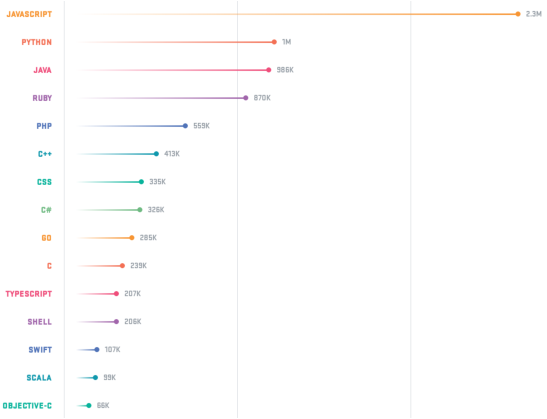
\includegraphics[scale=1.8]{github_2017.pdf}
 %\caption{As 15 linguagens mais usadas no GitHub em 2017. Fonte: \cite{githuboctoverse}}
 \caption{The 15 most used languages on GitHub in 2017. Source: \cite{githuboctoverse}}
 \label{fig:github_2017}
\end{figure}

\end{section}

\begin{section}{Parallelism in Compilation}

%O GCC é um compilador de código aberto amplamente usado tanto no meio
%acadêmico quanto na indústria. Por ser um grande projeto, o GCC contém uma
%linguagem própria para facilitar a adição de otimizações na geração de
%código, que em seguida é compilado em um único arquivo C, para (1)
%aproveitar as otimizações já implementadas no próprio compilador, e (2)
%evitar reescrever várias funcionalidades já implementadas. Infelizmente, este processo
%gera um gargalo na compilação do projeto em máquinas \textit{manycore}, pois o
%GCC não é capaz de compilar um arquivo em paralelo de maneira incremental.

%The GCC is a largely used Open Source compiler in both academic and industry
%environments. Being a large project, GCC has an additional language created to
%better express and facilitate optimizations in code generation, which is
%compiled into C++ to (1) reuse the optimizations already implemented in the
%compiler, and (2) avoid rewriting several functionalities already implemented.
%This process generates large files that must be compiled, causing a compilation
%bottleneck in the project because GCC is not capable of compiling a single file
%in parallel.

Currently, all parallelism in the compilation stage is provided either by the
GNU Make\footnote{https://www.gnu.org/software/make/}, which only provides a
per-file level granularity; or through the LTO infrastructure inside the compiler, which we
approach in Section \ref{chap:related_works}. The former, which we will label as
the \textit{classical compilation method}, may bottleneck the compilation in
manycore machines if there exists some file that dominates the compilation time.
The former may also have this bottleneck if the Whole Program Analysis (WPA) stage,
which runs serially, dominates the compilation time. While parallelizing
WPA is one way of tackling this problem, we have chosen to improve the parallelization
granularity on a single file compilation of \textit{classical compilation}.


%Atualmente, todo o paralelismo na fase de compilação é provido pelo GCC de
%duas maneiras distintas: ou pelo GNU Make\footnote{https://www.gnu.org/software/make/},
%que apenas fornece uma granularidade a nível dos arquivos; ou através da estrutura do
%LTO, que será abordada na Seção \ref{chap:related_works}. Esse gargalo pode parecer uma
%característica peculiar do projeto GCC, mas discussões com a comunidade levaram
%usuários a relatar o mesmo problema em seus projetos. Tal problema pode ser
%mitigado por um compilador que seja capaz de compilar um único arquivo em paralelo
%\citep{mailgcc}. Outra possível solução seria
%partir o arquivo em arquivos menores e utilizar o esquema de
%paralelismo já existente do GNU Make, mas isto implica em uma modificação na
%estrutura do projeto, o que pode não ser o ideal.

Since today the processors' manufacturers are increasing the power of their
products through parallelism over raw sequential power, compilers that can
profit from this resource could reduce the time taken when compiling a project
or even reduce execution time on script languages that rely on Just in Time
(JIT) compilation. It means a reduction in resource usage, such as
power, time, and thus money. So far, every parallelism found internally in
optimizing compilers was a consequence of a structure created to allow more
aggressive optimizations, such as the LTO \citep{glek2010optimizing}.

%Considerando que atualmente há uma tendência para que os processadores sejam
%cada vez mais paralelos, compiladores que usufruam deste recurso poderiam
%reduzir o tempo de compilação de um projeto, ou de uma suíte de testes que
%necessita recompilação antes de sua execução, economizando recursos no caso da
%computação ser cobrada por hora. Até então, o paralelismo empregado internamente
%em compiladores otimizadores foi consequência de uma estrutura criada para
%permitir otimizações mais agressivas e custosas, como o LTO
%\citep{glek2010optimizing}.

\end{section}

\begin{section}{Research Questions}\label{sec:rq}

%Deve ser observado que nem todos os processos de um compilador podem ser
%paralelizados. Compiladores operam em etapas que podem ser fortemente
%dependentes do resultado da etapa anterior. Por exemplo, ao compilar uma
%função em C, pode ser necessário saber se alguma outra foi declarada anteriormente; ou
%então o analisador sintático pode alterar um estado do analisador léxico para
%detectar variáveis de um novo tipo. Além disto, compiladores também se apoiam em algoritmos
%em grafos, cujo paralelismo é um desafio \citep{lumsdaine2007challenges}.

We must highlight that not every process inside a compiler can be parallelized.
Compilers that operate in steps can be strongly dependent on the resource
generated by some early pass.  For instance, when compiling a function in C, it
may be necessary to know if some function was declared early; or the syntactic
analyzer may change a state in the lexical analyzer to detect variables of a
new type. Not only that, but compilers also rely on graph algorithms, in
which parallelism is not trivial \citep{lumsdaine2007challenges}.

Therefore, this work is dedicated to the following research questions:

\begin{description}
    \item[\textit{RQ1}] - What is the main point of a compiler that can be improved with parallelism?
    \item[\textit{RQ2}] - What is the performance improvement after parallelizing a compiler?
	\item[\textit{RQ3}] - When compiling in parallel is faster than compiling sequentially?
	\item[\textit{RQ4}] - How does this impact the power consumption?
\end{description}

%Sendo assim, esse trabalho concentra-se em duas questões de pesquisas:
%\begin{description}
%    \item[\textit{QP1}] - Em que pontos um compilador pode usufruir de paralelismo?
%
%    \item[\textit{QP2}] - Qual é o ganho de desempenho ao paralelizar internamente um compilador?
%\end{description}

%essas questões de pesquisa visam propor uma alternativa ao LTO com foco
%em desenvolvimento incremental, e também cobrindo os casos onde o LTO produz binários menos
%eficientes através de melhorias no paralelismo do processo clássico de compilação.
%Para validar os resultados, este trabalho inclui a implementação no GCC de algumas das
%técnicas discutidas, além da utilização de técnicas de inferência estatística para
%análises no tempo total de compilação no projeto GCC e arquivos separados.

We present answers of these questions in the hope that they may be useful to software
developers so that they be aware of how compilers may impact the development
process of their projects, as well as compiler writers on how to improve
their software using parallelism. Thus, the main contribution of this work is
to provide ways to modify an industrial-scale compiler to
compile single files in parallel.

This work is divided into the following chapters: in Chapter
\ref{chap:fundamentacao}, we present some theoretical concepts regarding
Compiler Theory, the GCC,  and Parallel Computing to clarify some topics about this work.
Following that, Chapter \ref{chap:related_works} presents related work until
the state of art on this topic, with a brief discussion about their positive
and negative points. Then, Chapter \ref{chap:proposta} presents a general
version of the work, with an analysis of what needs to be improved,
contemplating the parallel architecture and the implementation planning, and presenting
our experiments about it later on Chapter \ref{cap:experiments}. Finally,
in Chapter \ref{chap:conclusions}, we present our conclusions about this work
and how it can be improved, with future works.

This work was supported by CAPES and Google Summer of Code (GSoC). For the
latter, we present our application plans in Appendix \ref{appendex1} for the threaded
parallelism project and Appendix \ref{appendix2} for the LTO parallelism project.  

%Este trabalho está dividido nos seguintes capítulos: no Capítulo
%\ref{chap:fundamentacao}, são apresentados conceitos teóricos como parte da
%Teoria de Compiladores e Computação Paralela para que seja possível
%compreender as questões acerca do trabalho.  Em sequência, o Capítulo
%\ref{chap:related_works} contém uma apresentação dos trabalhos relacionados
%a paralelismo de compiladores até o estado da
%arte nesse tópico, além de uma breve discussão sobre seus pontos positivos
%e negativos. Por fim, o Capítulo \ref{chap:proposta} apresenta uma visão geral
%do trabalho de fato, com uma análise de tempo consumido que permitiu
%identificar quais pontos necessitam de melhorias, além da
%proposta do trabalho, que contempla a arquitetura de paralelismo e o
%planejamento de sua implementação.

\end{section}

\chapter{Theoretical Background}
\label{chap:fundamentacao}

To avoid confusion regarding the various languages that the compiler works on,
we denote the following definitions on this work: Denote \textit{Source
Language}, as the language in which the code being compiled was originally
written; \textit{Intermediary Language} (IR) as the languages used internally in the
compiler; and \textit{Target Language} the language in which the compiler must
generate the code.

Compilers are large projects destined for the translation of source code
between distinct programming languages. Usually, compilers translate high-level
languages such as C, to assembly language, and those are the focus of our work.
We will not approach JIT compilers in this work, although they are very often
used in interpreted languages, such as Ruby or Python.

This chapter presents a brief introduction to the concepts used in this work.
In Section \ref{sec:parsing} we present a brief introduction about parsing
which are heavily used in a compiler. In Section \ref{sec:optimization} we
present all parts of the compiler pipeline to understand the compilation
phases. In Section \ref{sec:engineering} we discuss some software engineering
techniques that are employed when implementing compilers.  In Section
\ref{sec:gcc_compiler} we discuss the internals of the GCC compiler, from the
several Intermediate Representations of the compiler to the interaction between the parts.  In
\ref{sec:contributing} we present the details of the contributing process. In
Section \ref{sec:parallel_computing} we present some concepts from parallel
computing, which we use in this dissertation. And finally, Section
\ref{sec:power} briefly presents the concepts behind electrical power and energy
calculation, which we used in our experiments.

%Este capítulo apresenta uma breve introdução sobre os conceitos utilizados neste
%trabalho. Primeiro, são abordadas as partes do \textit{pipeline} de um compilador
%de maneira a entender os passos de compilação.
%Em seguida, discute-se como o compilador GCC apresenta esses tópicos implementados,
%além do seu uso no processo de compilação de um programa. Por fim, são
%apresentados alguns conceitos e algoritmos básicos sobre Computação Paralela.

%\begin{section}{Compiladores}

\begin{section}{Parsing}\label{sec:parsing}

Computer programs are written as a text file in some programming language,
which needs to be compiled or interpreted for execution. The first step of such
programs is to process the text file, validate the input with regard to the
language, and construct a data structure that is suitable for processing. This
process is named \textit{parsing}.

Parsing usually consists of two analysers: 
\begin{itemize}

\item \emph{Lexical Analysis}: responsible for reading a text file containing
the Source Code and splitting the words in the file into \textit{tokens}. As a
consequence, it is capable of applying some filters, \textit{e.g.} ignore commentaries,
identify numerical constants, remove unnecessary spaces, and replace a token
with another.  Lexical Analysers can also be used for macro expansion, as
implemented in the C preprocessor
(CPP)\footnote{https://gcc.gnu.org/onlinedocs/cppinternals/Lexer.html}.

Usually, Lexical Analysers are implemented using Deterministic Finite
Automatas, in which each acceptance state corresponds to a generated token.
This yields a fast, $O(n)$ algorithm for detecting tokens in the code, which
will be fed to the Lexical Analyser. There are even Lexical Analyser Generators
such as \textit{Flex}\footnote{https://www.gnu.org/software/flex/}, which are
extremely efficient.

\item \emph{Syntactic Analysis}: responsible to generate an Abstract Syntax
Tree (AST), inspecting the sequence of tokens provided by the Lexical Analyser,
or point out why the input string is invalid. The objective of a Syntatic
Analyser is to construct an AST by keeping track of the
reduction or derivation decisions with respect to the language grammar. The
decision of doing type analysis, checking for undefined usage of variables,
etc, can be done while building this AST, or postponed to a next stage, called
the Semantic Analysis.

Very often, these parsers are implemented either by emplying automatic
generated parsers such as \texttt{LALR}(1) algorithm provided by
\textit{Bison}\footnote{https://www.gnu.org/software/bison/}, or by
hand-implementing Recursive Descent parsers, which we present an example in
Figure \ref{fig:recursive-descent}. 

\end{itemize}

As an example of AST, Figure \ref{fig:ten-fact} illustrates a simple toy program in Java
that computes $10!$, and in Figure \ref{fig:ast-tenfact} we have a dump of its
AST.

\begin{figure}[ht]
      \begin{lstlisting}[
        language=pseudocode,
        style=pseudocode,
        style=wider,
        functions={},
        specialidentifiers={extern, call, public, static, class, void, String, int},
      ]
class Factorial {
    public static void main(String[] a) {
        System.out.println(new Fac().ComputeFac(10));
    }
}

class Fac {
    int teste;
    public int ComputeFac(int num) {
        int numxaux;
        int foo;
        if (num < 1)
            numxaux = 1;
        else
            numxaux = num * (this.ComputeFac(num-1));
        return numxaux;
    }
}
      \end{lstlisting}
	  \caption{Toy program to compute $10!$ in Java}
	  \label{fig:ten-fact}
\end{figure}


\begin{landscape}
\begin{figure}[ht]
    \begin{center}
     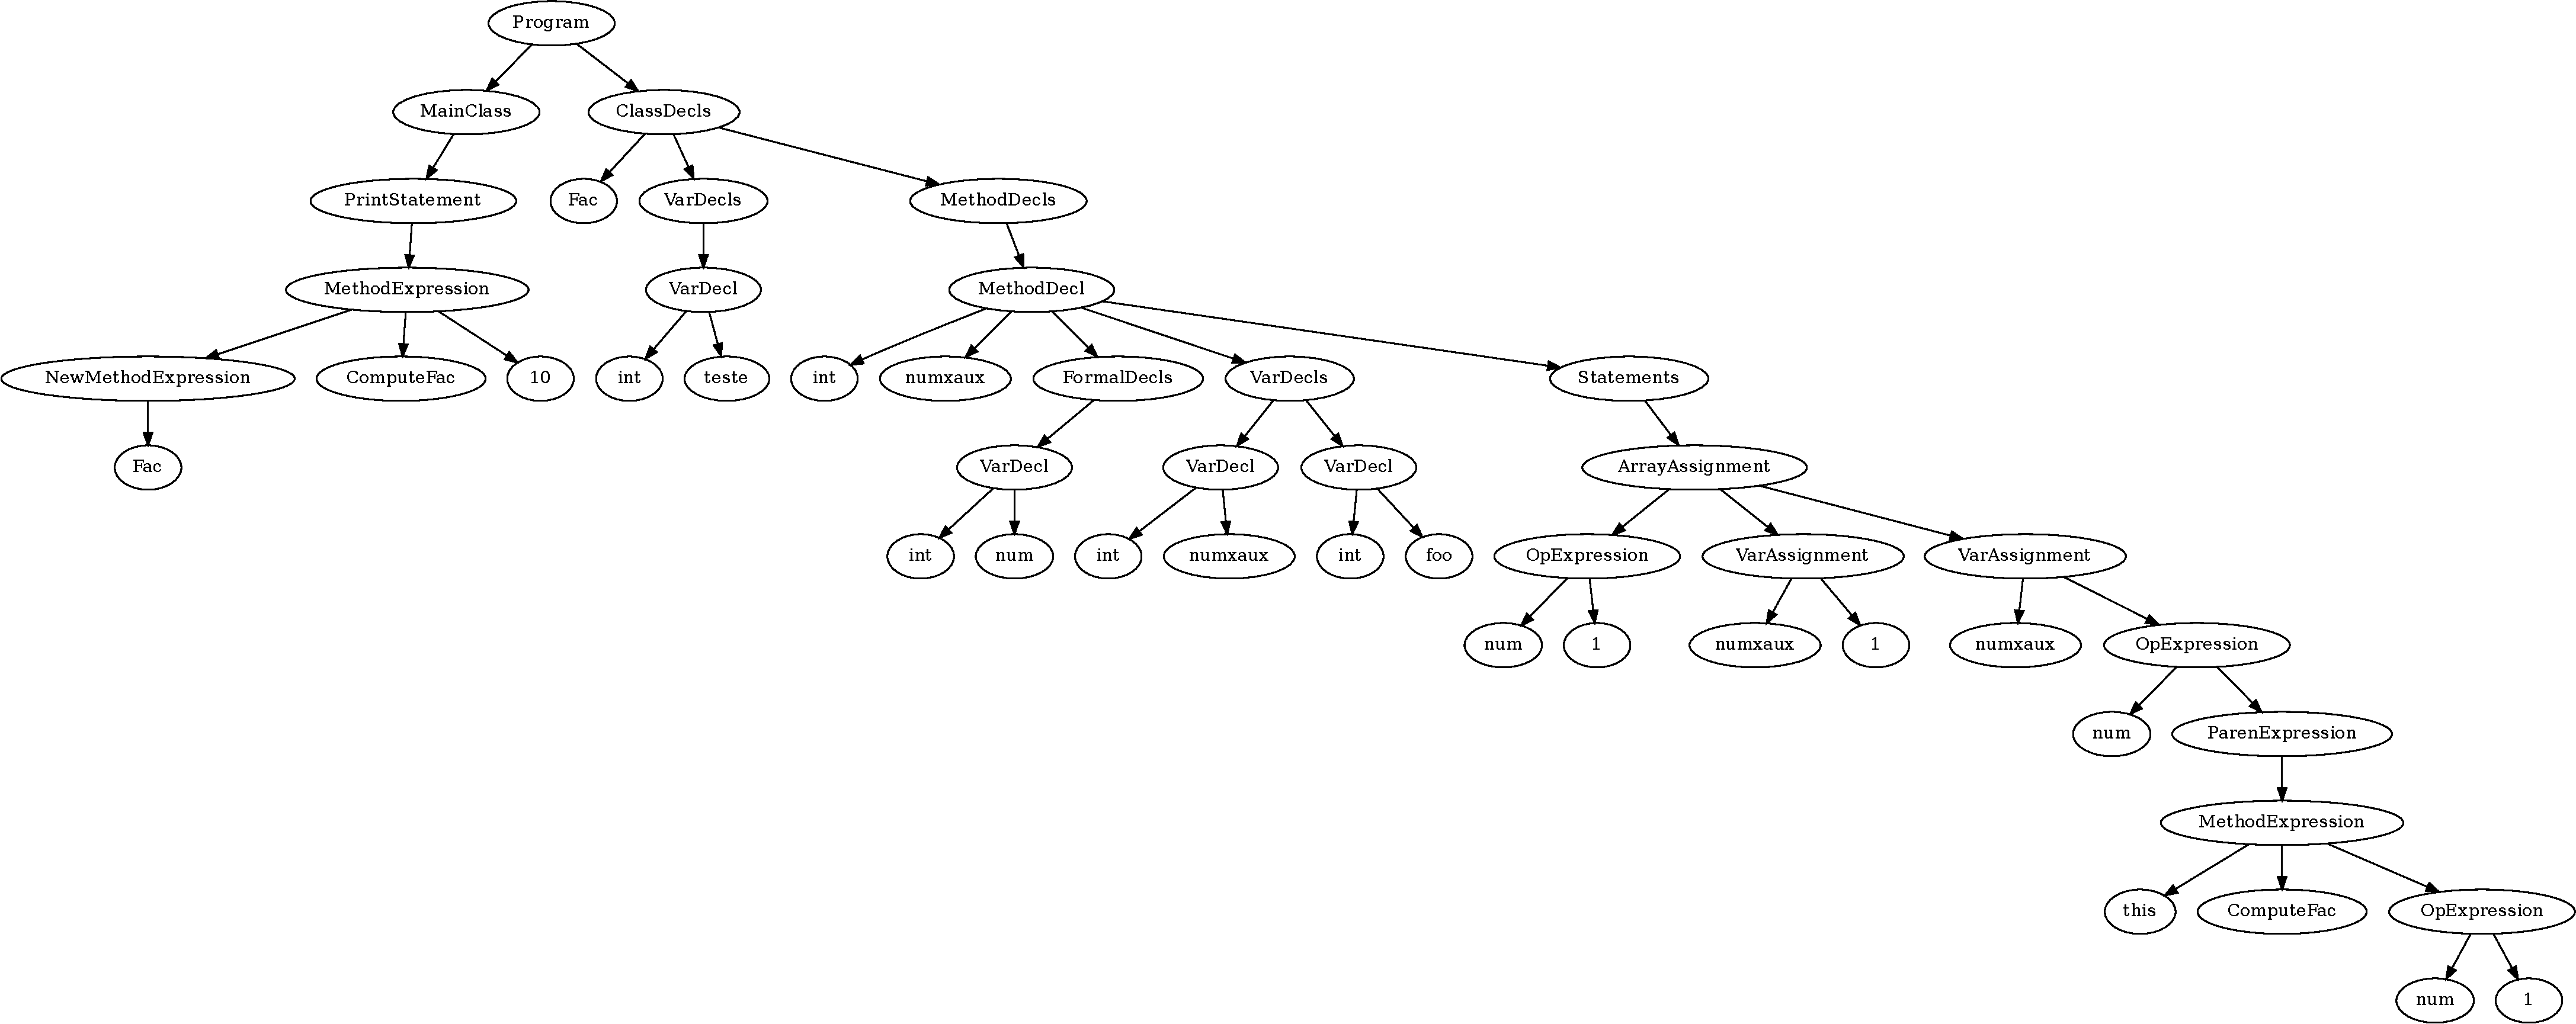
\includegraphics[width=0.8\paperheight]{ast.pdf}
	 \caption{Abstract Syntax Tree of Figure \ref{fig:ten-fact}}
	 \label{fig:ast-tenfact}
    \end{center}
\end{figure}
\end{landscape}

\end{section}

Another data structure constructed in this process is the Symbol Table.  The
Symbol Table, as the name suggests, is a table consisting of symbols
(variables, functions) with its declaration point, types, visibility, and other
information that the compiler writer might find useful. It is very often
constructed in this parsing process as the Syntactic Analyser detects variables
and functions, which may be used later to perform type checks and references to
undefined symbols. Figure \ref{fig:lexico_sintatico} illustrates how these
three pieces communicate with each other.

\begin{figure}
\tikzstyle{block} = [rectangle, draw, fill=white,
    text width=6em, text centered, rounded corners, node distance=9cm, auto, minimum height=2em]
\tikzstyle{line} = [draw, -latex]
\tikzstyle{cloud} = [draw, ellipse,fill=white, node distance=2cm,
    minimum height=2em]

%TODO: Adcionar a tabela de símbolos aqui.
\begin{center}
\scalebox{0.8}{
\begin{tikzpicture}[node distance = 3cm, auto]
    % Place nodes
    \node [block]                    (lexico) {Lexical Analyser};
    \node [block, right of = lexico] (sintatico) {Syntactic Analyser};
    \node [block] at (4.5, -2) (symtab) {Symbol Table};
    \coordinate [left of=lexico]     (fonte);
    \coordinate [right of=sintatico] (ast);

    % Draw edges
    \draw[->]    ([yshift=0.5em] lexico.east)       -- ([yshift=0.5em] sintatico.west) node[midway] {Token};
    \draw[->]    ([yshift=-0.5em] sintatico.west)   -- ([yshift=-0.5em] lexico.east)    node[midway] {next\_token()};
    \draw[->]    (fonte.west)                       -- (lexico.west)    node[pos=0, above] {Source Code};
    \draw[->]    (sintatico.east)                   -- (ast.west)   node[pos=1, above] {AST};
	\draw[->]    (sintatico.south)                  -- ([xshift=0.5em]symtab.north);
	\draw[->]    (lexico.south)                     -- ([xshift=-0.5em]symtab.north);

\end{tikzpicture}
}
\end{center}

\caption{Interactions between the Lexical, Syntactic Analyser and the Symbol Table}
\label{fig:lexico_sintatico}
\end{figure}

More details about how to construct parsers, what is a grammar in the context
of programming languages, and an brief introduction to parsing theory can be
seen in Appendix \ref{sec:apendix-parser}.


\begin{section}{Compiler Optimization}\label{sec:optimization}

Today industrial compilers are what we call to be an ``Optimizer Compiler'', because
it not only do a direct translation to another language, but because it
tries to generate faster code than the input code created by the programmer
while still maintaining its correctness.

There are several data structures and frameworks which is often used to
develop optimizations, which we briefly present here.

%Given a program, there are two disjoint set of optimizations in which we
%operate on:
%\begin{itemize}
%	\item \textit{Architecture-free Optimizations}: Any optimization that
%	does not require any interaction with anything specific about the target
%	machine in which the code is being compiled to. Example: \textit{constant
%	propagation}.
%
%
%	\item \textit{Architecture-dependent Optimizations}: Any optimization that
%	require interaction with something specific about the target machine in
%	which the code is being compiled to. Example: \textit{register allocation}.
%\end{itemize}
%
%Furthermore, we can also separate the set of all optimizations is two
%others disjoint sets:
%
%\begin{itemize}
%	\item \textit{Intraprocedural Optimizations}: Optimizations which only uses
%	information inside the function. Example: \textit{register allocation}.
%
%	\item \textit{Interprocedural Optimizations}: Any optimization that
%	require interaction with something specific about the target machine in
%	which the code is being compiled to. Example: \textit{function inlining}.
%\end{itemize}
%
%This last one is very interesting in the point of parallelization. Intraprocedural
%Optimizations can be run in parallel per function, as there is no dependency between
%two functions. Interprocedural, by the other hand, has no clear parallelization point.

\begin{subsection}{Three-Address Code Form}

One issue with large expressions is that it is very hard to find common
subexpressions and eliminate them. For instance, consider the mathematical
expression:
$$y = x \times x + x \times x $$
this expression can be simplified to $y = 2x^2$, but how
can a compiler know this? One could break this expression in the following
sequence of statements:
\begin{align}
t_1 &= x \times x \nonumber \\
t_2 &= x \times x \nonumber \\
y &= t_1 + t_2 \nonumber
\end{align}
now, some information is evident here. First is that $t_2 = t_1$,
and therefore $t_2$ is a completely unnecessary variable, and can be
eliminated from the program, which will lead to $y = t_1 + t_1$, which is
evident that can be simplified further to $y = 2 \times t_1$, which will lead
to the sequence of statements:

\begin{align}
t_1 &= x \times x \nonumber \\
y &= 2 \times t_1 \nonumber
\end{align}
which satisfy the following definition:
\begin{definition}
	A program is in Three-Address Code (3AC) format if every expression is
	in $c = a \texttt{<op>} b$ form, where $a, b, c$ are variables or
	literal constants.
\end{definition}

Not only used to detect common subexpressions, the 3AC representation is also
useful when allocating registers to variables, once instructions usually only
take two operands as argument (for instance, the \texttt{add} instruction in
x86). 

\end{subsection}

\begin{subsection}{Control-Flow Graph}

Programs consist of more than a linear sequence of statements, as there are
jumps, loops, and gotos, which we call \textit{flow-divergence}. Those
divergences can be modeled through a \textit{Control-Flow Graph}, which
illustrates jumps explicitly.

For example, consider the program in Figure \ref{fig:1-norm_program}.  Here,
the first two statements $i \leftarrow 0$ and $\textit{sum} \leftarrow 0$ are
always executed in the sequence, so there is no need to explicitly show any
kind of jump between these two statements. However, the \texttt{if} and
\texttt{else} will result in a \textit{flow-divergence} depending on the value
of \texttt{x[i]}, which is illustrated in Figure \ref{fig:1-norm_program:cfg}. 
\begin{figure}[ht]
\centering
  \begin{subfigure}[b]{0.40\textwidth}
      \begin{lstlisting}[
        language=pseudocode,
        style=pseudocode,
        style=wider,
        functions={},
        specialidentifiers={extern, call},
      ]
        function norm_1(x[n])
            sum := 0
			i := 0
            while (i < n) {
                if (x[i] < 0)
                    sum -= x[i]
                else
                    sum += x[i]
				i := i + 1
            }
            return sum
        end
      \end{lstlisting}
	  \caption{Program that computes the 1-norm of a vector}
	  \label{fig:1-norm_program}
  \end{subfigure}
  \begin{subfigure}[b]{0.40\textwidth}
    \tikzstyle{line} = [draw, -latex]
    \tikzstyle{node} = [draw, rectangle]
    \begin{center}
    \scalebox{0.5}{
    \begin{tikzpicture}[node distance = 2.3cm, minimum height = 1cm, auto]
        % Place nodes
        \node [node]                    (source) {$s_0$};
        \node [node, below of = source] (head) {while};
        \node [node, below of = head]   (check) {if};
        \coordinate[below of = check]            (c2);
        \node [node, left of = c2]  (true) {true};
        \node [node, right of = c2]   (false) {false};
        \node [node, below of = c2]   (merge) {$i \leftarrow i + 1$};
        \node [node, left of = head]   (return) {return};
        \coordinate[right of=false]    (c3);

        % Draw edges
        \draw[->]    (source)         -- (head);
        \draw[->]    (head)           -- (check);
        \draw[->]    (check)          -- (true);
        \draw[->]    (check)          -- (false);
        \draw[->]    (true)       -- (merge);
        \draw[->]    (false)      --  (merge);
        \draw    (merge.east) to [out=0, in=-90]  (c3);
        \draw[->]    (c3) to [out=90, in=0]  (head);

        \draw[->]    (head.west)  to [out=180, in=180] (return.east);
    \end{tikzpicture}
    }
    \end{center}
  \caption{Control-Flow Graph of the Program}
  \label{fig:1-norm_program:cfg}
  \end{subfigure}
\end{figure}
It is useful to model when those flow-divergences jumps will occur, which
motivates the definition of a \textit{basic-block}.

\begin{definition}
A \textbf{basic-block} is the maximum sequence of statements in which there is
no flow-divergence.
\end{definition}

For instance, both statements $i \leftarrow 0$ and $\textit{sum} \leftarrow 0$ belongs
to the same basic-block, as there are no \textit{flow-divergence} between
those two statements. However, \texttt{if (x[i] < 0)} and \texttt{sum += x[i]}
belongs to distinct basic-blocks. Figure \ref{fig:1-norm_program:cfg} shows
the basic block for the program. The definition of a Control-Flow Graph is
as follows.

\begin{definition}
	A Control-Flow Graph (CFGraph) $G = (V, E, s_0, F)$ is a directed-graph,
	where each $v \in V$ is a basic-block containing a list of statements,
	an edge $(u, v) \in E \ssq V \times V$ if the flow can jump from
	$u$ to $v$, $s_0 \in V$ is the source node, in which the execution
	starts, and $F \ssq V$ is the set of end blocks, in which there
	are no outgoing edges to other nodes.
\end{definition}

Control-Flow Graphs have several usages in compilers and static analyzers. For
instance, the analyzer can detect loops in codes that do not use any
conventional loop operands such as \texttt{while} or \texttt{for} (e.g. the
code has several \texttt{goto}s), and even detect unreachable code by verifying
if a certain node is reachable from the CFGraph source node. But its main usage
is on dataflow frameworks, which we will introduce in Subsection \ref{sec:dataflow}.

\end{subsection}

\begin{subsection}{Posets and Lattices}

One of the mathematical theories to model \textit{order between binary
relations} is called \textit{Lattice Theory}. One clear example of order in
mathematics is the set of all integers $\mathbb{Z}$ with the binary, partial
order relation $\leq$. However, when the set in which we are working on is
abstract, for instance which variables are live on some program point, such order relation turns out to be convoluted. Nevertheless, finding
such order in these abstract structures may be helpful.

\begin{definition}
A Partial Order $\sqsq$ over a set $S$ is a binary relation that is:
\begin{itemize}
	\item Reflexive: For all $s \in S$, $s \sqsq s$.
	\item Transitive: For all $q, r, s \in S$, if $q \sqsq r$ and $r \sqsq s$, then
	$q \sqsq s$.
	\item Anti-Symmetric: For all $r, s \in S$, if $r \sqsq s$ and $s \sqsq r$,
	then $r = s$.

A partially ordered set (poset) denoted by $\mathcal{P} = (S, \sqsq)$, is a
set $S$ with a partial order $\sqsq$. Furthermore, we say that $x \in \mathcal{P}$
if and only if $x \in S$.
\end{itemize}
\end{definition}

We can also define an operation on posets based on order, which is useful if
it denotes the amount of information we currently have so far.

\begin{definition}
Let $\mathcal{P} = (L, \sqsq)$ be a poset. A subset $S \ssq L$ has an
\textit{upper-bound} $l \in L$ if for every $r \in S$, then $r \sqsq l$.
Furthermore, $l$ is the \textit{least upper-bound} if for every other
upper-bound $x \in L$ of $S$, $r \sqsq x$.
\end{definition}

\begin{definition}
Let $\mathcal{P} = (L, \sqsq)$ be a poset. A subset $S \ssq L$ has an
\textit{lower-bound} $l \in L$ if for every $r \in S$, then $l \sqsq r$.
Furthermore, $l$ is the \textit{greatest lower-bound} if for every other
lower-bound $x \in L$ of $S$, $x \sqsq r$.
\end{definition}

\begin{definition}
The binary \textit{join} operator, denoted as $l \sqcup r$, is the
least upper-bound of the subset $\{r, s\}$ of a poset $\mathcal{P}$.
\end{definition}

\begin{definition}
The binary \textit{meet} operator, denoted as $l \sqcap r$, is the
greatest upper-bound of $\{r, s\}$ of a poset $\mathcal{P}$.
\end{definition}

One can clearly see that both $\sqcup$ and $\sqcap$ satisfies the
following three properties:

\begin{itemize}
	\item Idempotence: For all $r \in S$: $r \sqcup r = r$, and $r \sqcap r = r$ 
	\item Commutativity: For all $r, l \in S$: $l \sqcup r = r \sqcup l$, and
	$l \sqcap r = r \sqcap l$
	\item Associativity: For all $l, r, s \in S$: $(l \sqcap y) \sqcap s = l \sqcap (r \sqcap s)$
\end{itemize}

%Now, a desired condition to have in a poset is the \textit{ascending chain} (or
%\textit{descending chain}, according to the analysis) condition, so that we know
%that we know that eventually the propagation in the graph stabilizes.
%
%\begin{definition}
%A totally ordered chain $S = {s_1, s_2, \cdots}$ of a poset $\mathcal P$ is a
%\textit{ascending chain} if given two integers $1 \leq i \leq j$, then
%$s_i \sqsq s_j$. Analogously, $S$ is a \textit{descending chain} if
%$x_j \sqsq x_i$.
%\end{definition}

Notice that for a poset, the result of both $\sqcup$ and $\sqcap$ is not
required to be in the poset (\textit{i.e.} the operation is not closed).
That is the main difference between a poset and a \textit{lattice}.
If $\sqcap$ is closed, we have a \textit{meet semi-lattice}.

\begin{definition}
	A poset $\mathcal{P} = (L, \sqsq)$ is a \textbf{meet semi-lattice} if
	for every non-empty subset $S \ssq L$, $\left(\bigsqcap_{s \in S} s \right) \in L$.
\end{definition}

There is also structures which satisfies stronger claims, which is the case
of \textit{lattices} and \textit{complete lattices}.

\begin{definition}
	A poset $\mathcal{P} = (L, \sqsq)$ is a \textbf{lattice} if for every
	non-empty finite subset $S \ssq L$, both $\left(\bigsqcup_{s \in S} s\right) \in L$
	and $\bigsqcap_{s \in S} s \in L$.
\end{definition}

\begin{definition}
	A poset $\mathcal{P} = (L, \sqsq)$ is a \textbf{complete lattice} if
	for every subset $S \ssq L$, both $\left( \bigsqcup_{s \in S} s \right) \in L$
	and $\left(\bigsqcap_{s \in S} s \right) \in L$.
\end{definition}

It is also useful to denote the greatest and the smallest element of a lattice.

\begin{definition}
	The \textbf{top} element of a lattice $\mathcal{L}$ is $\top = \bigsqcup_{l \in \mathcal{L}} l$. Similarly, the \textbf{bottom} element is $\bot = \bigsqcap_{l \in \mathcal{L}} l$.
\end{definition}

However, for dataflow frameworks, it is not required to work on a complete
lattice. A meet semi-lattice is enough.

We can also define functions over a lattice in a similar way that functions can
be defined in $\mathbb{Z}$. From all functions that could be defined over a
lattice, we are interested in monotone functions, which helps to ensure that
some analysis ends after a finite number of iterations.

\begin{definition}
	A function $f:\mathcal{L} \longrightarrow \mathcal{L}$ is monotonic if and only if
	for $x, y \in \mathcal{L}$:
	$$x \sqsq y \Rightarrow f(x) \sqsq f(y)$$.
\end{definition}

Lattices have an important role in the formal definition of dataflow
frameworks, as they are often used to prove that the analysis always halts with
some result for every input program.
For instance, the fact that the meet operation always gives a result closer to
the bottom element guarantees that frameworks using a meet semilattice will
always converge to a result.

\end{subsection}

\begin{subsection}{Dataflow Analysis}\label{sec:dataflow}

Dataflow Analysis is a technique to collect and propagate information across a
Control-Flow Graph. It is used not only in compilers but also in static code
analysis in general in the field of Software Engineering.

When analyzing a program's function, it is useful to know at a certain point,
what properties do hold to decide for an optimization.  Incorrectly guessing
some property may result in an incorrect transformation. Therefore, it is
useful to employ a way to propagate information across the Control-Flow Graph
of a function. This is where Dataflow Analysis is useful.

Given a Control-Flow Graph $G = (V, E, s_0, F)$ of a program, construct a
complete or meet lattice $\mathcal{L}$, which represents a set of possible
information that is true in a certain point of a program.  Then, we define a
set of \textit{flow functions} $\mathcal{F}_G = \{f_1, f_2, \cdots, f_{|V|}\}$,
where $f_v: \mathcal{L} \longrightarrow \mathcal{L}$, for each node $v \in V$.
These functions will generate, destroy, or transform information contained in
each vertex of the graph. These functions must be of the form of
\textit{forward analysis}, which yields Equation \ref{eq:forward}, or
\textit{backward analysis}, which yields Equation \ref{eq:backward}.

\begin{equation}\label{eq:forward}
	\texttt{in[} v \texttt{]} = \begin{cases}
	  BI,& \text{if } v = s_0 \\
	  \bigsqcap_{p \in \text{pred}(v)}f_p(\texttt{in[}p\texttt{]}) ,& \text{otherwise} \\
	\end{cases}
\end{equation}

\begin{equation}\label{eq:backward}
	\texttt{out[} v \texttt{]} = \begin{cases}
	  BI,& \text{if } v \in F \\
	  \bigsqcap_{p \in \text{succ}(v)}f_p(\texttt{out[}p\texttt{]}) ,& \text{otherwise} \\
	\end{cases}
\end{equation}

Equations \ref{eq:forward} and \ref{eq:backward} can be solved by
\textit{propagation}, just applying the equation to each vertex until there is
no more new information being generated or destroyed (in other 	words, the
equation \textit{converges}). Some tricks can be employed for a faster
convergence, \textit{e.g.}, start propagation from $s_0$ in forward analysis,
and from any $v \in F$ in the backward analysis.  Algorithms for solving those
equations in a general way can be found in \citep{khedker2009data}.

Figure \ref{fig:functions_dataflow} illustrates how each function of
$\mathcal{F}_G$ are related to each node of the $G$. Furthermore, Figure
\ref{fig:meet_dataflow} illustrates how the meet operator $\bigsqcap$ is used
to combine the information generated by the predecessors and send it to the
successors of a node, for the \textit{forward analysis} case.

\begin{figure}[ht]
\centering
  \begin{subfigure}[b]{0.40\textwidth}
	 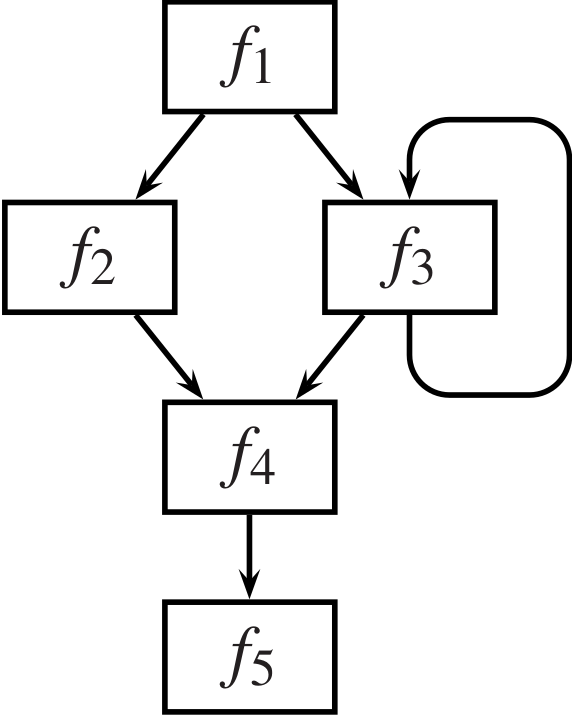
\includegraphics[scale=0.2]{functions_dataflow.png}
	  \caption{Dataflow Flow Functions. One for \\ each vertice of $G$. \citep{khedker2009data}}
	  \label{fig:functions_dataflow}
  \end{subfigure}
  \begin{subfigure}[b]{0.40\textwidth}
	 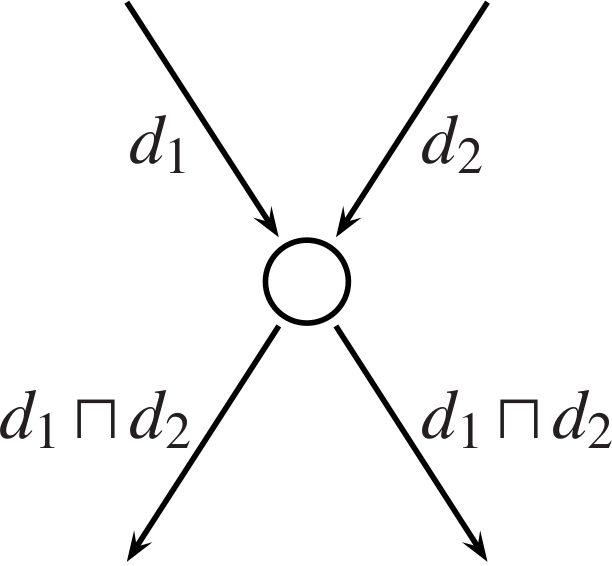
\includegraphics[scale=0.2]{meet_dataflow.png}
	  \caption{Meet operation on a vertice, combining the generated information. \citep{khedker2009data}}
	  \label{fig:meet_dataflow}
  \end{subfigure}
  \label{fig:dataflow}
\end{figure}

	Therefore, in an abstract way, we can define a dataflow framework instance as
	\begin{definition}
		An instance of dataflow framework is a 4-uple $(G, \mathcal{L}, \bigsqcap, \mathcal{F}_G)$,
		where
		\begin{itemize}
			\item $G = (V, E, s_0, F)$ is a Control-Flow Graph.
			\item $\mathcal{L}$ is a meet semi-lattice satisfying the descending chain condition.
			\item $\bigsqcap$ is the meet operator of $\mathcal{L}$.
			\item $\mathcal{F}_G = \{f_1, f_2, \cdots, f_{|V|}\}$ is the set of monotonic transfer
			functions, one for each node $v \in V$, of the form of Equation \ref{eq:forward} or \ref{eq:backward}.
		\end{itemize}
	\end{definition}

Dataflow frameworks have an important role in compilers and software static
analysis, as they are often used to model problems that require information to
be propagated through the CFGraph. Several problems can be solved by finding a
solution to a dataflow equation, such as constant folding, liveness analysis,
pointer alias, and so on. We will present liveness analysis as an example, once
it is used in the register allocation phase.

\begin{subsubsection}{Liveness Analysis}

One example of a problem that can be solved with dataflow analysis is the
\textit{liveness analysis}.
The purpose of it is to find, given a point in a CFGraph, if a certain variable
will be used in the future. This step is important to the register allocation
phase because if a certain variable is used in the future, we may need to keep
its value in a register for future use. If the variable is not live anymore,
then we can use that register to hold another variable, thus improving register
usage in the final code.  \cite{khedker2009data} defines the liveness
analysis formally as:

\begin{definition}

Let $G = (V, E, s_0, F)$ be a CFGraph and $\mathbb{V}$ be the set of all
variables of $G$. A variable $x \in \mathbb{V}$ is \textbf{live} at a program
point $v \in V$ if there exists a path from $v$ to $w \in F$ which contains a
use of $x$ which is not preceeded by its definition.
\end{definition}

Therefore, a CFGraph $G$, a dataflow framework instance for this would be:
$(G, \mathcal{L}, \bigsqcap, \mathcal{F}_G)$, where
\begin{itemize}
	\item $\mathcal{L} = (2^\mathbb{V}, \supseteq)$, where $\mathbb{V}$ is the set of variables in the function represented by $G$.
	\item $\bigsqcap$ is the union operator $\bigcup$.
	\item $F_G = \conj{\texttt{in[} v \texttt{]}}{v \in V}$ where
	$\texttt{in[} v \texttt{]} = (\texttt{out[} v \texttt{]} - \texttt{kill[} v \texttt{]}) \cup \texttt{gen[} v \texttt{]}$.
\end{itemize}
which yields the dataflow equation:
\begin{equation}\label{eq:liveness}
\begin{split}
	\texttt{in[} v \texttt{]} &= (\texttt{out[} v \texttt{]} - \texttt{kill[} v \texttt{]}) \cup \texttt{gen[} v \texttt{]} \\
	\texttt{out[} v \texttt{]} &= 
	\begin{cases}
	  \emptyset,& \text{if } v \in F \\
	  \bigcup_{p \in \text{succ}(v)}\texttt{in[}p\texttt{]} ,& \text{otherwise} \\
	\end{cases}
\end{split}
\end{equation}

In this equation, $\texttt{gen[} v \texttt{]}$ represents the variables which
turns to be live at vertex $v$, and $\texttt{kill[} v \texttt{]}$ are the
variables which liveness are no longer valid at vertex $v$. For instance,
consider the CFGraph in Figure \ref{fig:cfg_liveness}. Here, we work on the set
$\mathbb{V} = \{a, b, c, d\}$.  We present the solution of Equation
\ref{eq:liveness} is presented in Table \ref{fig:table_cfg} using the
propagation technique. There, for instance, we can see that $d$ is not used
anywhere in the program because $d \not\in \ttt{out[}n_1\ttt{]}$. This means
that the variable $d$ can be discarded from the program, and therefore no
register or memory space is necessary to hold this variable.

\begin{figure}
\centering
	 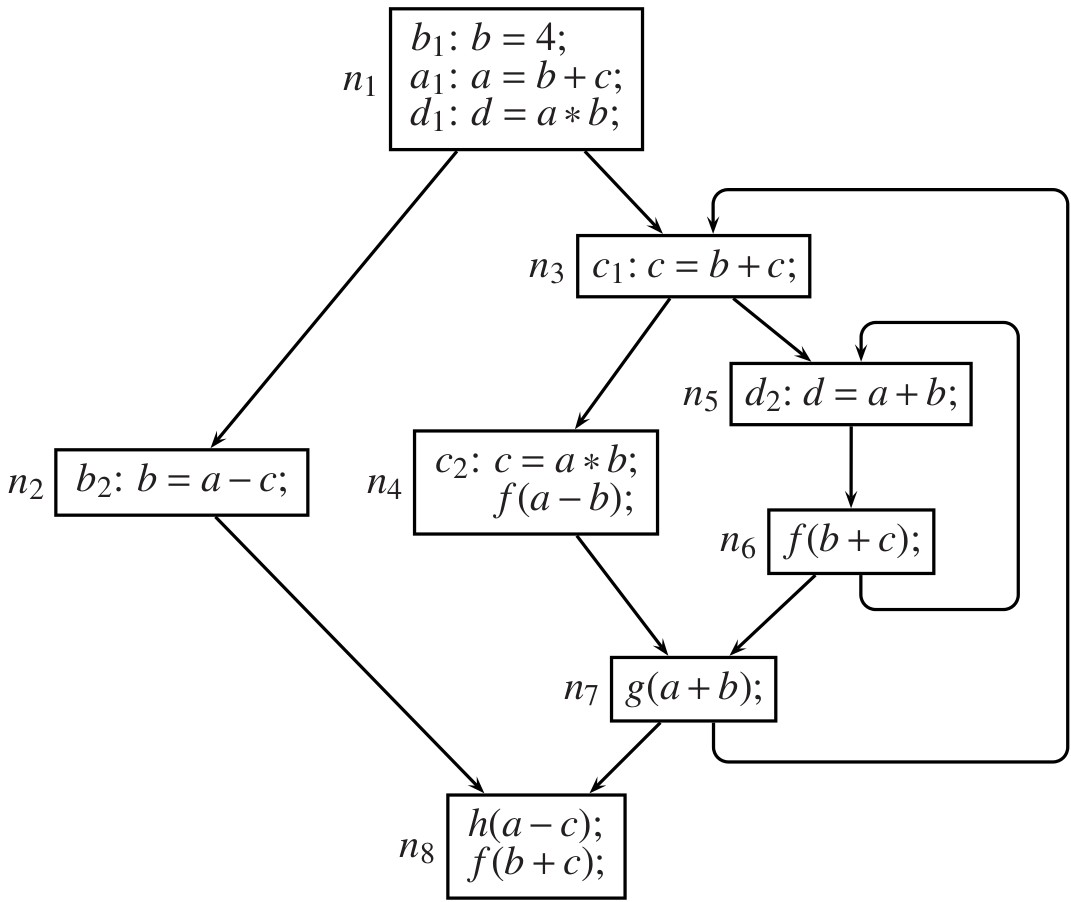
\includegraphics[scale=0.3]{cfg_liveness.png}
	  \caption{Example of CFGraph of a program function \citep{khedker2009data}.}
	  \label{fig:cfg_liveness}
\end{figure}

\begin{table}[]
\begin{tabular}{|c|c|c|c|c|c|c|}
\hline
\multirow{3}{*}{Vertex} & \multicolumn{2}{c|}{\multirow{2}{*}{Local Generation}}  & \multicolumn{4}{c|}{Global Information}                             \\ \cline{4-7} 
                        & \multicolumn{2}{c|}{}                                   & \multicolumn{2}{c|}{Iteration 1} & \multicolumn{2}{c|}{Iteration 2} \\ \cline{2-7} 
                        & $\texttt{gen[}n\ttt{]}$                        & $\ttt{kill[}n\ttt{]}$                   & $\ttt{out[}n\ttt{]}$             & $\ttt{in[} n\ttt{]}$             & $\ttt{out[}n\ttt{]}$             & $\ttt{in[} n\ttt{]}$            \\ \hline
$n_8$                   & $\{a, b, c\}$                & $\emptyset          $            & $\emptyset$               & $\{a, b, c\}$    & $\emptyset          $     & $\{a, b, c\}$    \\ \hline
$n_7$                   & $\{a, b\}$                   & $\emptyset          $            & $\{a, b, c\}$     & $\{a, b, c\}$    & $\{a, b, c\}$     & $\{a, b, c\}$    \\ \hline
$n_6$                   & $\{b, c\}$                   & $\emptyset          $            & $\{a, b, c\}$     & $\{a, b, c\}$    & $\{a, b, c\}$     & $\{a, b, c\}$    \\ \hline
$n_5$                   & $\{a, b\}$                   & $\{d\}      $            & $\{a, b, c\}$     & $\{a, b, c\}$    & $\{a, b, c\}$     & $\{a, b, c\}$    \\ \hline
$n_4$                   & $\{a, b\}$                   & $\{c\}      $            & $\{a, b, c\}$     & $\{a, b\}   $    & $\{a, b, c\}$     & $\{a, b\}   $    \\ \hline
$n_3$                   & $\{b, c\}$                   & $\{c\}      $            & $\{a, b, c\}$     & $\{a, b, c\}$    & $\{a, b, c\}$     & $\{a, b\}   $    \\ \hline
$n_2$                   & $\{a, c\}$                   & $\{b\}      $            & $\{a, b, c\}$     & $\{a, c\}   $    & $\{a, b, c\}$     & $\{a, c\}   $    \\ \hline
$n_1$                   & $\{c\}   $                   & $\{a, b, d\}$            & $\{a, b, c\}$     & $\{c\}      $    & $\{a, b, c\}$     & $\{c\}      $    \\ \hline

\end{tabular}
\caption{Solving the Equation \ref{eq:liveness} for Figure \ref{fig:cfg_liveness} 
\citep{khedker2009data}.}
\label{fig:table_cfg}
\end{table}

\end{subsubsection}

\end{subsection}

\begin{subsection}{Dominator Tree}
	One data structure used on optimization are
	\textit{dominator trees}. First we must define what \textit{domination} means:

	\begin{definition}
		Let $G = (V, E, s_0, F)$ be a Control-Flow Graph and $u, v \in V$. We say
		that $u$ \textbf{dominates} $v$ if every path from $s_0$ to $v$ go through
		$u$.
	\end{definition}

	That means that if some node $u$ dominates $v$, then it is certain that, in
	the current thread, the code in $u$ will be executed before $v$.
	\cite{georgiadis2006finding} presents a forward dataflow equation
	to compute the set of all dominators of a node:


\begin{equation}\label{eq:domtree_dataflow}
\begin{split}
	\texttt{dom[} v \texttt{]} &= 
	\begin{cases}
	  \{v\},& \text{if } v = s_0 \\
	  \left(\bigcap_{p \in \text{pred}(v)}\texttt{dom[}p\texttt{]}\right) \cup \{v\} ,& \text{otherwise} \\
	\end{cases}
\end{split}
\end{equation}

	However, instead of solving Equation \ref{eq:domtree_dataflow}
	every time we want to know if there is such dominance, or avoid
	holding a table containing \textit{every} dominator of a node,
	it is convenient to build a data structure that can quickly query
	such information. Such data structure is the \textit{dominator tree}
	of a CFGraph. Figure \ref{fig:domtree} presents the dominator tree of the CFGraph
	presented in Figure \ref{fig:cfg_liveness}.

\begin{figure}
\centering
\begin{tikzpicture}[sibling distance=3em,
  every node/.style = {shape=circle,
    draw, align=center}]]
  \node {$n_1$}
    child { node {$n_2$} }
    child { node {$n_3$}
      child { node {$n_4$} }
      child { node {$n_5$}
        child { node {$n_6$} } }
      child { node {$n_7$} } }
  	child { node {$n_8$} };
\end{tikzpicture}
\caption{Dominator tree of Figure \ref{fig:cfg_liveness}}
\label{fig:domtree}
\end{figure}


	Dominator trees are often used to build the Static Single Form (SSA) of a
	CFGraph, to detect loops in the Control-Flow Graph, and in several loop
	optimizations, such as hoisting constant variables outside of a loop,
	detecting induction variables, and so on.
	\cite{appel2004modern} provides algorithms to detect loops using the
	CFGraph, which is useful when the language supports \texttt{goto}s. A
	faster algorithm (but complex than the dataflow equation) algorithms to
	build the Dominator tree of a CFGraph is presented by
	\cite{georgiadis2006finding}.

\end{subsection}

\begin{subsection}{Static Single Assignment Form (SSA)}

Consider the following sequence of statements:
\begin{align}
x &= 2 \nonumber \\
y &= x \times x \nonumber \\
y &= y + 1 \nonumber \\
y &= 1 \nonumber
\end{align}

Clearly, the second and third statements can be discarded, and the first
and last statements can be discarded as well if there is no further use of $x$ and $y$ in the program. However, how can the compiler know that? SSA form makes this clear. The idea is that variables can not be redefined, only new variables can be created, which motivates the following definition.

\begin{definition}
	A program is in SSA form if there is exactly one assignment for each
	variable.
\end{definition}

We can convert the presented sequence of statements in this form by creating
a new variable for each left-hand-side of the assignment. Therefore, if a
variable has multiple definitions, we can eliminate that by creating a new
variable for that value, which yields
\begin{align}
x &= 2 \nonumber \\
y_1 &= x \times x \nonumber \\
y_2 &= y_1 + 1 \nonumber \\
y_3 &= 1 \nonumber
\end{align}

This will lead to the variable $y_2$ being unused because it is nowhere present
on the right-hand side of any assignment (has no use in the \textit{def-use}
chain), meaning that it can be discarded; which will then imply that $y_1$ will
be unused and can be discarded as well.

However, SSA form can get trickier to implement if there are jumps in the
programs, which is often the case with \texttt{if} and \texttt{while}
statements. In Figure \ref{fig:code_normal}, the value of \texttt{u}
depends upon which path the execution was taken, which depends on the
\textit{condition}. The solution fot this is to introduce a $\phi$-function,
which will select the correct variable. Figure \ref{fig:code_ssa_form}
illustrates this.

\begin{figure}[ht]
    \centering
    \begin{subfigure}[b]{0.40\textwidth}

        \begin{lstlisting}[
            language=pseudocode,
            style=pseudocode,
            style=wider,
            functions={},
            specialidentifiers={extern, call},
            ]
            if (condition) then
                a = -1;
            else
                a = 1;
            end
            u = a*v;
        \end{lstlisting}
        \caption{\label{fig:code_normal}}
    \end{subfigure}
    \begin{subfigure}[b]{0.40\textwidth}
        \begin{lstlisting}[
                language=pseudocode,
                style=pseudocode,
                style=wider,
                functions={},
                specialidentifiers={extern, call, PHI},
              ]
            if (condition) then
                $a_1$ = -1;
            else
                $a_2$ = 1;
            end
            $a_3$ = $\phi$($a_1$, $a_2$)
            u = $a_3$*v;
        \end{lstlisting}
        \caption{\label{fig:code_ssa_form}}
\end{subfigure}
\caption{A program (a) and its SSA representation (b)}
\end{figure}

However, this illustration explains little about when to
place $\phi$ functions. A way of determining it is to use
the \textit{dominance frontier criteria}

\begin{definition}
	Let $G = (V, E, s_0, F)$ be a CFGraph and $u, v \in V$. We say that
	$u$ \textbf{strictly dominates} $v$ if $u$ dominates $v$, but
	$u \neq v$. We denote that $u$ idom $v$.
\end{definition}

\begin{definition}
	The \textbf{dominance frontier} of a node $x \in V$ is the set of all nodes $w \in V$
	such that $x$ dominates a predecessor of $w$, but does not strictly dominate $w$ \citep{appel2004modern}.
	Or, in set theory notation:
\end{definition}
\vspace*{-1cm}
	$$\texttt{dfront[}x\texttt{]} = \conj{w \in V}{x \text{ dom } y \text{ for some } y \in \text{pred}(w) \text{ and } y \text{ does not sdom } w}$$

This definition looks blurry, but it can be easily understood as the
\textit{border of nodes where the dominance stops}.  Figure
\ref{fig:dom_frontier} illustrates this concept with a plot of the dominated
nodes of $v_5$ in the beige area and the dominance frontier in the green area.

\begin{figure}[ht]
 \centering
 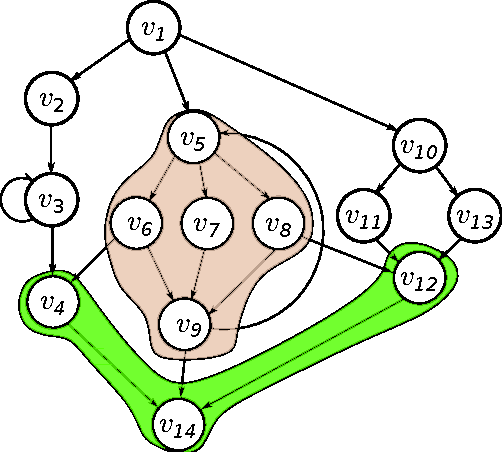
\includegraphics[scale=1.0]{dom_frontier.pdf}
 \caption{Dominance frontier of node $v_5$. Beige is dominated by $v_5$. Green is in dominance frontier of $v_5$.}
 \label{fig:dom_frontier}
\end{figure}

The criteria to place $\phi$-functions are the following: When a node $x$ contains a defintion
of a variable $a$, then any node $z$ in the dominance frontier of $x$ needs a $\phi$ function
for $a$. \citep{appel2004modern}.

SSA makes the optimizing compiler fast because it avoids relying on dataflow
bit vector equations to compute \textit{def-use}. Instead of finding whenether a
certain variable was redefined, or detecting which version of the variable is being
used, SSA simply enforces that a variable has a single definition. This makes
several optimizations easy.

For instance, dead-code elimination can simply check if a variable has no use.
If a variable had previously two definitions and the second has no use, SSA
will transform this variable into two other variables and the second one
would have no use, and therefore could be elminated \citep{appel2004modern}.

\end{subsection}

\begin{subsection}{Callgraphs and Interprocedural Analysis}

Some optimizations require interaction with other functions, one clear example
of this is the \textit{function inlining} optimization. When there is a
function call, the call itself consumes time, and therefore it may be
interesting to copy and paste the content of the function being called and
remove the call at all.  Therefore, a data structure is required to model the
interactions between functions.

That is the purpose of a \textit{Callgraph}: each vertex denotes a function,
and each edge represents a call between two functions. 

\begin{definition}
	A Callgraph is a graph $G = (V, E)$, where $V = \{f_1, f_2, \cdots, f_{|V|}\}$
	are the set of functions, and $E = \conj{(u, v)}{u, v \in V}$ are the set
	of edges representing a function call. Given $(u, v) \in E$, this means
	that $u$ (the \textbf{caller}) calls $v$ (the \textbf{callee}).
\end{definition}

Figure \ref{fig:call_graph} gives an example of a Callgraph. When applying
Interprocedural Optimizations, each vertex can also hold some sort of
\textit{summary} of the function instead of the entire function, because the
program being compiled often is large enough that there is not sufficient
memory to hold the contents of the functions in the host machine which is
compiling the code. This is the case when working with
the Link Time Optimization (LTO) technique.

There are some extensions to the dataflow frameworks to work on Interprocedural
Optimizations \citep{khedker2009data}, however, they require complete
information about the function in memory, which may not be present in this
stage on compilers such as GCC \citep{gcc_ipa}.

\begin{figure}[ht]
\centering
  \begin{subfigure}[b]{0.40\textwidth}
      \begin{lstlisting}[
        language=pseudocode,
        style=pseudocode,
        style=wider,
        functions={},
        specialidentifiers={extern, call},
      ]
        extern function g,h

        function f()
            call $g$
            call $h$
        end

        function main()
            call $f$
            call $h$
        end
      \end{lstlisting}
  \end{subfigure}
  \begin{subfigure}[b]{0.40\textwidth}
    \tikzstyle{line} = [draw, -latex]
    \tikzstyle{node} = [draw, circle]
    \begin{center}
    \scalebox{1.0}{
    \begin{tikzpicture}[node distance = 2.3cm, minimum height = 1cm, auto]
        % Place nodes
        \node [node]                    (main) {\texttt{main}};
        \node [node, below of = main]        (f) {\texttt{f}};
        \node [node, below of = f]           (g) {\texttt{g}};
        \node [node, right of = f]           (h) {\texttt{h}};

        % Draw edges
        \draw[->]    (main)           -- (f);
        \draw[->]    (f)              -- (g);
        \draw[->]    (f)              -- (h);
        \draw[->]    (main)           -- (h);
    \end{tikzpicture}
    }
    \end{center}
  \end{subfigure}
  \caption{A program and its callgraph}
  \label{fig:call_graph}
\end{figure}

Callgraphs are often used to model interprocedural optimizations, such as
function inlining, as it models the call relationship between functions. For
instance, inlining can increase the program size in bytes tremendously if the
function is called from multiple locations, which can further slow down the
program due to instruction cache and page faults.

\end{subsection}

\begin{subsection}{Register Allocation}
Registers are very fast, but small memories inside a processor, which data is
required to be loaded for operations like add, subtract, multiply, etc. These
memories are a very scarce resource in a processor, and therefore it
must be administered carefully.

A good (near-optimal) register allocation can hugely speed up the program
because it avoids unnecessary accesses between the CPU and the computer's
memory, and this is the purpose of the register allocation.

The idea of this step is to represent the variables in the IR so that it can be
easily mapped into the CPU registers. Therefore, since the IR can have an
infinite number of variables, the goal here is to rewrite the code such that it
uses no more temporaries than there are registers in the machine. For example,
consider the Figure \ref{fig:register_ir}. In (a), we have a sketch of the
program, and in (b) we have the rewrite using at most 4 registers.

\begin{figure}[ht]
    \centering
    \begin{subfigure}[b]{0.40\textwidth}
		\begin{align}
			a &= b + c      \nonumber \\
			d &= a \times e \nonumber \\
			f &= d + 1      \nonumber
		\end{align}
        \caption{\label{fig:code_normal}}
    \end{subfigure}
    \begin{subfigure}[b]{0.40\textwidth}
		\begin{align}
			r_1 &= r_2 + r_3      \nonumber \\
			r_1 &= r_1 \times r_4 \nonumber \\
			r_1 &= r_2 + 1        \nonumber
		\end{align}
        \caption{\label{fig:code_register}}
\end{subfigure}
\caption{A program (a) and its presentation on registers (b)}
\label{fig:register_ir}
\end{figure}

	However, how can a compiler \textit{know} when a certain variable will not
	be used anymore, and we can replace the register with computation of some
	kind? By using the \textit{liveness analysis}.

\begin{definition}
	Let $t_1$ and $t_2$ be two temporaries variables. If $t_1$ and
	$t_2$ are live at a given point $p$, then $t_1$ and $t_2$ can not
	share the same register.
\end{definition}

This information is used to build an \textit{interference graph}, which an
example is presented in Figure \ref{fig:interf_graph}.

\begin{definition}
	An interference graph $G = (V, E)$ is a graph where $V = \mathbb{V}$ is the
	set of variables in the program, and $E \ssq V \times V$ are the set of
	edges. An edge $(u, v) \in E$ if $u$ and $v$ are simultaneously live at
	at some program point $p$.
\end{definition}

\begin{figure}
    \tikzstyle{line} = [draw, -latex]
    \tikzstyle{node} = [draw, circle]
    \begin{center}
    \scalebox{1.0}{
    \begin{tikzpicture}[node distance = 2.3cm, minimum height = 1cm, auto]
        % Place nodes
        \node [node]                         (d) {$d$};
        \node [node, right of = d]           (b) {$b$};
        \node [node, right of = b]           (f) {$f$};
        \node [node, below of = d]           (c) {$c$};
        \node [node, right of = c]           (e) {$e$};
        \node [node, right of = e]           (a) {$a$};

        % Draw edges
        \draw        (b)              -- (c);
        \draw        (c)              -- (e);
        \draw        (e)              -- (b);
        \draw        (e)              -- (a);
    \end{tikzpicture}
    }
    \end{center}
	  \caption{Interference Graph of Figure \ref{fig:register_ir}.}
	  \label{fig:interf_graph}
\end{figure}

After the interference graph is constructed, it is possible to know how many
registers it is necessary and where to allocate once the graph is colored.
Graph coloring, unfortunately, is an NP-Complete problem
\citep{karp1972reducibility}, which implies that a heuristic is necessary to
solve this problem.

\cite{appel2004modern} shows one heuristic. Suppose that the target machine has
$k$ available registers. Once the interference graph has been built, select one
node $v$ with degree $d(v)$ such that $d(v) < k$. The idea is around the fact that
if $G' = G - \{v\}$ can be colored, then so do $G$ because one can simply select
a color distinct from every node that $v$ is adjacent to, which results in a 
recursive coloring algorithm. This is called \textit{simplify}.

However, nothing is preventing that there are no nodes $v$ such that
$d(v) \geq k$. In this case, there is no alternative other than allocate the
variable in memory. This is called \textit{spilling}.

Once this process is completed, variables can be renamed accordingly to their
register, or memory location.

\end{subsection}

\begin{subsection}{Instruction Selection}
An important step in the final translation process is the
\textit{instruction selection}. Most processors (such as x86) have more
than a way to translate a statement to machine code, for instance, 
assigning a variable to zero. One could use \texttt{mov reg, 0}, or
even \texttt{xor reg, reg}, but the latter one is faster as it takes fewer
cycles to execute. This is specially important for CISC-based processors,
which a sequence of instructions can be replaced with a single instruction,
resulting in a faster program. Detecting such cases is the main issue here.

There are several techniques to select instructions. One of the simplest
is the \textit{macro translation}, where each statement is replaced
by the final code locally for each line of the IR. This has the advantage
of being a fast way to implement a way to translate the code, but
very often generate poor final code, as illustrated in
Figure \ref{fig:macro_exp}. Some optimizations can be employed
to improve the result of such translations, such as
\textit{peephole optimization}, which search in a small window unnecessary memory operations that annulate themselves.

\begin{figure}
\tikzstyle{block} = [rectangle, draw, fill=white,
    text width=15em, text centered, rounded corners, node distance = 1cm and 1cm, auto, minimum height=2em]
\tikzstyle{line} = [draw, -latex]
\tikzstyle{cloud} = [draw, ellipse,fill=white, node distance=2cm,
    minimum height=2em]

\begin{center}
\scalebox{0.8}{
\begin{tikzpicture}
    % Place nodes
    \begin{scope}[node distance = 1cm and 5cm]
    \node [block]                  (c1) {$\textit{fib}_i = \textit{fib}_{i-1} + \textit{fib}_{i-2}$};
    \node [block, below=of c1]     (c2) {$\textit{fib}_{i-2} = \textit{fib}_{i-1}$};
    \node [block, below=of c2]     (c3) {$\textit{fib}_{i-1} = \textit{fib}_{i}$};
    \end{scope}

    \node [block, right=of c1]     (asm1) {\texttt{mov eax, DWORD [ebp-8]} \\ \texttt{mov ebx, DWORD [ebp-12]} \\ \texttt{add eax, ebx} \\ \texttt{mov [ebp-4], eax}  };
    \node [block, right=of c2]     (asm2) {\texttt{mov eax, DWORD [ebp-8]} \\ \texttt{mov [ebp-12], eax}};
    \node [block, right=of c3]     (asm3) {\texttt{mov eax, DWORD [ebp-4]} \\ \texttt{mov [ebp-8], eax}};

    % Draw edges
    \draw[->]    (c1.east)        -- (asm1.west);
    \draw[->]    (c2.east)        -- (asm2.west);
    \draw[->]    (c3.east)        -- (asm3.west);
\end{tikzpicture}
}
\end{center}
\caption{Macro instruction selection for x86. Intel syntax.}
\label{fig:macro_exp}
\end{figure}

Another approach is to treat the IR as a \textit{tree}, then try to
pattern-match a set of nodes in which this pattern has an efficient
translation.  Figure \ref{fig:tree-matching} illustrates this process, in
general.

\begin{figure}
\centering
	 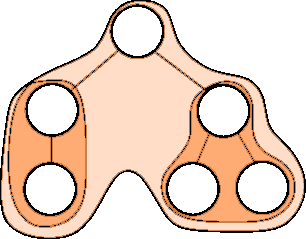
\includegraphics[scale=1.0]{tree_replace.pdf}
	  \caption{Illustration of a tree-matching algorithm}
	  \label{fig:tree-matching}
\end{figure}

There are some algorithms for matching such trees. One, proposed by
\cite{glanville1978}, describes a Context-Free Grammar to translate the IR into
assembler language. However, in many machines, such grammar will always be
ambiguous, implying that such grammars will not pass the $\mathcal{DK}_1$ test
(see Section \ref{sec:bottom-up}), either by \textit{shift-reduce} or
\textit{reduce-reduce} conflicts.

	The solution of this problem is as follows:

	\begin{itemize}
		\item On \textit{shift-reduce} conflicts, always choose to shift. The intuition is that larger patterns will result in more optimal code since it allows more information to be gathered by the parser. However, the parser could simply select to \textit{shift} when it should have 	\textit{reduce}d. Therefore, either backtracking is necessary here when the parser takes the wrong decision, or the grammar designer provides additional rules to avoid such cases.

\item On \textit{reduce-reduce} conflicts, it selects the rule with yields the
longest pattern. The reason is also that the longest patterns will generate
better code. However, even this can also result in a parsing error. The
solution is to devise a rule in which can be used as a fallback, and the
authors provide a way to automatically find such a rule.

	\end{itemize}

Such parsers are very interesting because, given a way to express what the
parser should produce and the cost of these productions, one can quickly
implement a new \textit{backend} to the compiler.  The main issue, however, is
the high number of states required by the
parser \citep{blindell2016instruction}, which often turns it impractical.

There is a way to optimally select instructions on a tree using a technique
called \textit{dynamic programming} \citep{ripken1977formale}. The idea is that given a node $n$, it is enough to first consider to minimize the cost
of the child and then try to minimize the cost of $n$. Mathematically, let
$P_n$ the set of patterns possible to be applied to $n$. Therefore, the
minimal cost $\texttt{PD[}n\texttt{]}$ is:

\[
    \texttt{pd[}n\texttt{]} =
     \begin{cases}
       \min_{p \in P_n} \texttt{cost[}p\texttt{]}  &\quad\text{if } n \text{ is leaf}\\
       \min_{p \in P_n} \texttt{cost[}p\texttt{]} + \sum_{f \in \text{succ}(p)} \texttt{pd[}f\texttt{]} &\quad\text{otherwise}\\
     \end{cases}
\]

Another way of selecting instructions is through Directed Acyclic Graph. Its
advantage, when compared to trees, is that it can represent common
subexpressions, but unfortunately optimal algorithms for this representation
are NP-complete \citep{koes2008near}. The majority of techniques employed here
are greedy, as in \cite{llvm_insn_selection}.

Finally, a more detailed discussion on instruction selection is presented
by \cite{blindell2016instruction}.

\end{subsection}

\end{section}

\begin{section}{Software Engineering in Compilers}\label{sec:engineering}

%Para evitar confusões a respeito das diferentes linguagens que um compilador
%trabalha em seus muitos estágios, é adotado a seguinte nomenclatura neste trabalho:
%Denote \textit{Linguagem Fonte} como sendo a linguagem
%na qual o código fonte do programa a ser compilado foi originalmente escrito;
%\textit{Linguagem Intermediária} uma das linguagens internas do compilador; e
%\textit{Linguagem Alvo} a linguagem na qual o compilador deverá gerar código.


%Compiladores são grandes projetos destinados a tradução de códigos fonte
%entre distintas linguagens de programação. Normalmente, compiladores traduzem
%linguagens de alto nível, como C, para linguagens mais próximas da máquina,
%como a linguagem de montagem - embora isso não seja uma regra pois existem
%compiladores cuja única tarefa é realizar uma tradução entre duas linguagens
%de alto nível.

%Compiladores também costumam otimizar
%o código que passam por eles, aplicando diversas heurísticas de
%maneira a acelerar o código a ser produzido, substituindo trechos de código por
%outros mais eficientes, reordenando as instruções do programa, etc.

Compilers are large programs. Because of this, there is a great interest in
avoiding rewriting a compiler when a new language is proposed, or when new
hardware is created. For that, compiler writers usually adopt the following
modularization \citep{redhat} \citep{llvm}, as illustrated by Figure
\ref{fig:compiler_arch}:

%Por serem programas extremamente grandes, existe um grande interesse em evitar
%reescrever um novo compilador
%sempre que uma nova linguagem é proposta, ou um novo \textit{hardware} é criado.
%Para isso, a seguinte modularização é largamente adotada por projetistas de
%compiladores \citep{redhat} \citep{llvm}, conforme ilustrado na Figura \ref{fig:compiler_arch}:
%

\begin{itemize}

\item A Front End for each Source Language. In this module are executed the
lexical and syntactical analysis to construct the Abstract Syntax Tree (AST)
and populating the Symbol Table. Following that, this structure is converted to
another compiler's IR.

\item A Middle End, responsible for applying several \textit{hardware independent}
optimizations to the already converted IR code. A \textit{hardware independent}
optimization is such that there are no dependency with regard to the Target
Language (often, assembler of some processor). Example: \textit{constant propagation}.

\item A Back End for each Target Language, responsible to translate the IR to
the Target Language and applying \textit{hardware dependent} optimizations,
such as register allocation and instruction selection. A \textit{hardware dependent}
optimization is such that there \textit{is} a dependency with regard to the
Target Language. Example: \textit{register allocation}.

\end{itemize}

%\begin{itemize}
%    \item Um \textit{Front End} para cada Linguagem Fonte.
%	Neste módulo são executadas as análises léxica e sintática, com a
%        finalidade de construir uma Árvore de Sintaxe Abstrata (AST), para que em
%seguida, ela seja convertida para uma Linguagem Intermediária do compilador.
%
%    \item Um \textit{Middle End}, responsável por aplicar diversas otimizações
%independentes de arquitetura no código já convertido para a Linguagem Intermediária.
%
%    \item Um \textit{Back End} para cada linguagem alvo, responsável por converter a linguagem intermediária
%na linguagem alvo. Aqui outras otimizações específicas da linguagem alvo são realizadas,
%como alocação de registradores e seleção de instruções.
%\end{itemize}

However, this modularization is completely optional: older compilers destined
to simply doing a direct translation between languages, such as the UNIX C
Compiler, do not have an IR \citep{ritchie1979tour}. Not only that, several
textbooks about compilers do not mention the Middle-End part, being a part of
the Back-End of the compiler \citep{dragonbook}. Not adopting this
modularization simplifies the project, but also complicates the insertion of
new programming languages, as well as adding support to new hardware.

%Porém, essa modularização é opcional: compiladores mais antigos destinados a fazer uma
%conversão direta entre duas linguagens, como o UNIX C Compiler, não costumam usar uma linguagem
%intermediária \citep{ritchie1979tour}, além de diversos livros-texto não mencionarem tal módulo, fundindo suas
%funcionalidades com o \textit{Back End} \citep{dragonbook}. Não adotar tal metodologia
%simplifica o projeto, mas dificulta a inserção de suporte a novas
%linguagens de programação.


\begin{figure}
\tikzstyle{block} = [rectangle, draw, fill=white,
    text width=6em, text centered, rounded corners, node distance=5cm, auto, minimum height=2em]
\tikzstyle{line} = [draw, -latex]
\tikzstyle{cloud} = [draw, ellipse,fill=white, node distance=2cm,
    minimum height=2em]

\begin{center}
\scalebox{0.8}{
\begin{tikzpicture}[node distance = 3cm, auto]
    % Place nodes
    \node [block]                      (front_c)    {C Front-End};
    \node [block, below of=front_c]    (front_cpp)  {C++ Front-End};
    \node [block, below of=front_cpp]  (front_fort) {Fortran Front-End};
    \node [block, right of=front_cpp]  (middle)     {Middle-End};
    \node [block, right of=middle]     (back_x86)   {x86 Back-End};
    \node [block, above of=back_x86]   (back_arm)   {ARM Back-End};
    \node [block, below of=back_x86]   (back_ppc)   {PPC Back-End};


    \coordinate [left of=front_c]    (c_code);
    \coordinate [left of=front_cpp]  (cpp_code);
    \coordinate [left of=front_fort]  (fort_code);

    \coordinate [right of=back_x86] (x86_code);
    \coordinate [right of=back_arm] (arm_code);
    \coordinate [right of=back_ppc] (ppc_code);

    % Draw edges
    \draw[->]    (front_c.east)     to [out=0,in=180] ([yshift=0.5em]  middle.west);
    \draw[->]    (front_cpp.east)   to [out=0,in=180] (middle.west);
    \draw[->]    (front_fort.east)  to [out=0,in=180] ([yshift=-0.5em] middle.west);

    \draw[->]    ([yshift=-0.5em] middle.east)  to [out=0,in=180] (back_ppc.west);
    \draw[->]    (middle.east)                  to [out=0,in=180] (back_x86.west);
    \draw[->]    ([yshift=0.5em] middle.east)   to [out=0,in=180] (back_arm.west);

    %\draw[->]    (sintatico.west)   -- (lexico.east)    node[midway] {próximo\_token()};
    %\draw[->]    (fonte.west)       -- (lexico.west)    node[pos=0, above] {Código Fonte};
    %\draw[->]    (sintatico.east)   -- (ast.west)       node[pos=1, above] {Árvore Abstrata};
\end{tikzpicture}
}
\end{center}

\caption{Compiler Architecture}
\label{fig:compiler_arch}
\end{figure}

%\begin{subsection}{\textit{Front-End}}
\begin{subsection}{Front-End}

A Front-End is a module responsible for direct interaction with the code
written in the Source Language, which means from a Software Engineering
perspective, for adding support to a new Source Language, it is enough to write
a new Front-End. It is also possible that some classes are shared between
frontends, which may be the case of a compiler that supports both C and C++.

%Um \textit{Front End} é um módulo responsável por interagir diretamente com o
%código escrito na Linguagem Fonte a ser compilado. Ele costuma ser único
%para cada Linguagem Fonte, ou seja, para inserir suporte a uma nova
%Linguagem Fonte, basta implementar um novo \textit{Front End}, mas é
%possível que algumas classes sejam
%compartilhadas, como no caso de um compilador que dê tanto para C quanto para e C++.


As a first step, the Front-End performs a lexical and syntactical analysis for
generating an AST and verify if the input text belongs to the language. It is
also responsible for printing parsing errors in a way that the user can easily
understand them. The Front-End also populates the Symbol Table of the compiler
with symbols that it has seen so far when compiling the program for checking if
there are references to undefined symbols. These three pieces (the Lexical
Analyser, the Syntactic Analyser, and the Symbol Table) frequently communicate
with each other, as illustrated in Figure \ref{fig:lexico_sintatico}.

%Como primeiro passo, \textit {Front End} realiza uma análise
%léxica e sintática, com a finalidade de gerar uma AST e verificar
%se o texto dado como entrada realmente pertence à linguagem.
%Estes dois analisadores se comunicam constantemente, conforme ilustrado na Figura
%\ref{fig:lexico_sintatico}.


%    Primeiro, a análise léxica é responsável por ler o arquivo
%de texto contendo o código fonte, e quebrar as palavras em \textit{tokens}, que
%serão alimentados para o analisador sintático. Por consequência, ele é capaz de
%realizar alguns filtros, \textit{e.g}. ignorar os comentários, identificar constantes
%numéricas, eliminar espaços desnecessários, e substituir um \textit{token} por
%outro.
%Analisadores léxicos também podem ser usados para substituição
%de macros, como implementado pelo preprocessador do C
%(CPP)\footnote{https://gcc.gnu.org/onlinedocs/cppinternals/Lexer.html}.

%Geralmente, os Analisadores Léxicos são implementados utilizando autômatos
%por diversos motivos, entre eles sua atrativa complexidade computacional
%$O(n)$, onde $n$ é o tamanho da entrada, pela existência de algoritmos
%para converter expressões regulares em autômatos \citep{thompson}, e pela
%existência de algoritmos para minimização de estados de um autômato
%\citep{hopcroft1971n}. Isto possibilita que geradores de analisadores léxicos
%como o \texttt{Flex}\footnote{https://www.gnu.org/software/flex/}
%sejam bastante eficientes.

After the AST is generated and the Semantic Analysis is completed, it is often
converted to an IR, where Target-Independent Optimizations are performed. This
yields the control to the Middle-End of the compiler.

\end{subsection}

\begin{subsection}{Middle End}

The Middle-End is responsible to work on one or more IR(s) of the compiler. If
there are checks which can be postponed in the Front-End to this stage, it is
preferable, once it avoids these checks on every Source Language's Front-End.

Here, we construct data structures in which might be necessary for the
hardware-independent optimizations, such as the Control-Flow Graph, the
Callgraph, the SSA representation, and so on. After that, the compiler indeed
runs these optimizations.

The Middle End is where the most effort is spent in development. Every new
optimization here will improve the code for every target machine that the
compiler supports.

After this optimization process, the code in this IR can be further transformed
into other IR to something that is more closely related to the target hardware.
After that, the control is passed to one of the compiler's Back End, where it
will be transformed to the final language.

\end{subsection}

\begin{subsection}{\textit{Back End}}

The \textit{Back End} is responsible for the final translation to the target
language, as well as hardware-dependent optimizations. Therefore, it is also
responsible for selecting instructions optimally (or close to) as well as
selecting registers from the best way possible for the program's variable.

The Back End should be implemented in a way that it can simply be switched for
another without any modification to the Middle End. With this, the code can be
easily compiled to another target language.

After the Back End has done its processing, the final code is issued and the compilation is complete.

\end{subsection}

\begin{subsection}{Compilation Passes}

Compilers, however, can optimize for several metrics, not only execution time.
Industrial compilers also very often support \textit{optimization for size} for
embedded systems, or even \textit{optimize for power consumption}, which can be
interesting for both embedded systems and data centers. Therefore, some
optimizations may be executed while others must be disabled depending on what
are you optimizing to. This is where a simple but powerful modularization comes
into, the \textit{compiler passes}.

A pass is simply a set of rules to run in the IR. For instance, one pass
could match and replace a set of statements in the IR for a faster one,
or even simply collect information about some function, such as the
\textit{cyclomatic complexity}.

Passes can be easily implemented using classes, and all passes are structured
in a queue. Each pass should receive the information in which it is working on
(for instance, a data structure representing the current function being worked
on) and has a \textit{gate} method, which will determine if this optimization
will or will not be run, according to some compilation flags or even with some
information collected with some previous pass. It is even possible that there
are subpasses to a pass, containing its own queue of passes. Figure \ref{fig:pass_queue}
illustrates this queue. 

\begin{figure}

\tikzstyle{block} = [rectangle, draw, fill=white,
    text width=6em, text centered, rounded corners, node distance=5cm, auto, minimum height=2em]
\tikzstyle{line} = [draw, -latex]
\tikzstyle{cloud} = [draw, ellipse,fill=white, node distance=2cm,
    minimum height=2em]

\begin{center}
\scalebox{0.8}{
\begin{tikzpicture}[node distance = 3cm, auto]
    % Place nodes
    \node [block]                      (pass1)    {Pass 1};
    \node [block, right of = pass1]    (pass2)    {Pass 2};
    \node [block, below of = pass2]    (subpass1)    {Subpass 2 1};
    \node [block, right of = subpass1] (subpass2)    {Subpass 2 2};
    \node [block, right of = pass2]    (pass3)    {Pass 3};

    % Draw edges
    \draw[->]    (pass1.east)     to [out=0,in=180] (pass2.west);
    \draw[->]    (pass2.east)     to [out=0,in=180] (pass3.west);
    \draw[->]    (pass2.south)    to  (subpass1.north);
    \draw[->]    (subpass1.east)  to [out=0,in=180] (subpass2.west);
\end{tikzpicture}
}
\end{center}
\caption{Pass Queue}
\label{fig:pass_queue}
\end{figure}

\end{subsection}
\end{section}

\begin{section}{The GCC Compiler}\label{sec:gcc_compiler}

The GNU Compiler Collection, also known as GCC, is a project started by
Richard Stallman with the first public release in March of 1987. Back then,
it only supported C language but already allowed code generation for
several architectures \citep{gcc_first_ver}.

Today, GCC supports several source languages, such as C, C++, Fortran, Go, Ada;
and several architectures, such as i386, amd64, riscv, arm, ppc, and pdp-11.
GCC is also an optimizer compiler, which means it can modify the input code to
generate a more efficient version without changing the program semantic. This
is archived through its several IR: GENERIC, GIMPLE, and RTL. The compiler run
optimization passes on each of these IR.

%Hoje, o GCC fornece suporte a diversas Linguagens Fonte como C, C++, Fortran, Go, Ada,
%e várias arquiteturas, como i386, amd64, riscv, arm, ppc, pdp-11. O GCC também
%é um compilador otimizador, ou seja, ele é capaz de alterar o código fornecido
%pelo usuário com a finalidade de gerar código mais eficiente, sem alterar a semântica do programa. Isso é
%possível por conta das várias Linguagens Intermediárias implementadas no
%GCC: GENERIC, GIMPLE, e RTL. O compilador executa vários
%passos de otimização em cada uma dessas linguagens intermediárias.

\begin{subsection}{GENERIC}

GENERIC is a IR that allows to represent any function in the program with
trees.  Such language is a superset of all functionalities and attributes
that every Source Language has, for instance, attributes such as
\texttt{volatile} in C, C++, or even Fortran matrix sum or product. Other
functionalities are more common to every language, such as function calls,
variable declaration, class, expressions, statements, and others
\citep{generic}.

%    O GENERIC é uma linguagem intermediária que possibilita representar quaisquer
%funções do programa através de árvores. Tal linguagem é um superconjunto
%das funcionalidades e atributos que cada Linguagem Fonte contém, por exemplo, atributos
%como \texttt{volatile} de C e C++ contém uma representação nessa linguagem.
%Outras funcionalidades são: chamadas de função, declaração de variáveis, classes,
%funções, expressões, entre outros \citep{generic}.

This language contains a faithful representation of the program closest to what
was written by the programmer, meaning that there are no modifications in the
program. This language is not in 3AC or SSA form, it is only there for an easy
translation to GIMPLE, the hardware-independent IR of GCC in which most
optimizations are done, and to make the development of a Front End easily.
However, that does not mean that optimizations can not be applied here.

There is a match-and-replace mechanism in GCC supporting GENERIC. This
mechanism is very simple: it searches for a chain of statements in the IR for a
pattern and then replaces for another. Such patterns are expressed in the file
\texttt{gcc/match.pd}. This simple mechanism allows several bitwise logic and
mathematical simplifications that can give a significant speedup in the code in
particular cases \citep{sinatan}.


%    Essa linguagem contém uma representação mais próxima de como o programa foi
%escrito pelo programador, ou seja, não são feitas modificações nas expressões.
%Sendo assim, essa linguagem
%intermediária não se enquadra nas categorias de \textit{Three Address Code},
%ou \textit{Static Single Assignment} pois isso demanda modificações no código.
%O objetivo principal dessa linguagem
%é facilitar a tradução para a próxima linguagem intermediária, a GIMPLE, e assim
%facilitar o desenvolvimento dos \textit{Front End} do compilador, mas isso não
%significa que otimizações não possam ser aplicadas aqui.

%    O GCC possui um mecanismo de substituição de nós em sua representação
%interna, dando suporte a árvore construída em GENERIC. Esse mecanismo é simples: o
%compilador procura por uma cadeia de nós na árvore, buscando padrões,
%como especificado no arquivo \texttt{gcc/match.pd}, e os substitui pelo o que
%foi instruído na regra de substituição. Esse mecanismo, embora simples, permite
%com que diversas simplificações matemáticas sejam implementadas no código, o
%que pode significar uma melhora de até $10\times$ em casos particulares
%\citep{sinatan}.

	Finally, each Front End of GCC is responsible for translating the source
	code for this intermediate language. To visualize a program in this representation,
	compile the program with the flag \texttt{-fdump-tree-original}. However,
	the documentation is very clear that C and C++ frontends translate
	directly to GIMPLE \citep{gimple}.

\end{subsection}

\begin{subsection}{GIMPLE}

GIMPLE is another IR from GCC, basically consisting of conversion from GENERIC
to a 3AC representation, having a further step into lowering this
representation to construct the Control-Flow Graph and the SSA form. As
GENERIC, GIMPLE is general enough to represent every attribute from all Source
Languages supported by the compiler. This representation is based on SIMPLE, an
IR from McCAT compiler \citep{gimple}.

%O GIMPLE é outra linguagem intermediária do GCC, basicamente consistindo na
%conversão de GENERIC para \textit{Three Address Code}, havendo ainda um passo
%posterior adicionando uma representação SSA a esta linguagem. Assim como o
%GENERIC, a GIMPLE também é geral o suficiente para representar os atributos
%de todas as Linguagens Fonte de cada \textit{Front End}.  Essa linguagem
%intermediaria é baseada na linguagem SIMPLE, do compilador McCAT \citep{gimple}.

It is in GIMPLE that all hardware-independent optimizations are performed.
GIMPLE has an \textit{Application Programming Interface} (API) for interacting
with statements, tree nodes, the Control-Flow Graph, SSA nodes, and the
Callgraph. GIMPLE has two states, the ``high'' state, with lexical scopes and
nested expressions, and ``low'' state, exposing all implicit jumps and
Exception Handles (EH) regions, removing the lexical scopes, merging similar
return statements, and convert try-catch control flows to exception regions.

GIMPLE code can be dumped by using the flag \texttt{-fdump-tree-gimple},
or even \texttt{-fdump-tree-ssa} to write the SSA representation on the
disk.

\end{subsection}

\begin{subsection}{Register Transfer Language}

	The last IR of GCC is the \textit{Register Transfer Language} (RTL).
	The syntax of this language ressembles Lisp, where expressions
	are represented by a list of commands \citep{rtl}.


%    Por fim, a última linguagem intermediária do compilador GCC é a
%\textit{Register Transfer Language} (RTL). A sintaxe dessa linguagem
%tem inspiração no Lisp, onde as expressões são representadas por uma
%lista de comandos .

	RTL is a language that aims to be as close as the assembler language
	as possible, while still being generic enough to be compatible with
	every target language of GCC. It represents a machine with an infinite
	number of registers that will be correctly selected to a machine
	register on the register allocation pass, or allocated in memory.

%    A RTL é uma linguagem que visa ser extremamente próxima da linguagem
%de montagem, mas ainda sendo genérica o suficiente a ponto de ser compatível
%com todas as Linguagens Alvo do GCC.
%Para isso, ela representa uma máquina com infinitos
%registradores, que serão alocados em registradores reais no passo correspondente.
%Caso a arquitetura alvo não tenha o número necessário de
%registradores, as variáveis deverão ser guardadas em memória. Por exemplo,
%no caso do i386, elas deverão ser salvas na pilha. Esse processo é conhecido
%como \textit{Register Spilling}.

	The final step is the assembler emission once all optimizations were
	performed in RTL. This will employ a macro translation instruction
	selection algorithm to convert RTL functions, statements, and expressions
	into assembler. That is why RTL optimizers are necessary here, to avoid
	generating very poor assembler code \citep{gcc_insns_selection}.

%    Essa é a última Linguagem Indermediária antes da geração do código final. O
%\textit{Back end} transformará o código nessa linguagem para a Linguagem Alvo
%substituindo uma sequência de instruções em RTL por uma sequência de instruções
%na Linguagem Alvo. Essa escolha segue um sistema
%de custos no qual o compilador procura escolher uma sequência de instruções
%que minimiza a soma do custo total da tradução.
%
%    Na arquitetura i386, as regras de substituição estão implementadas
%em \texttt{gcc/config/i386/i386.md}, com o sistema de custos definido
%na \texttt{struct processor\_costs}, no arquivo \texttt{gcc/config/i386/i386.h}.
%Cada processador da arquitetura i386 deve definir o custo de cada instrução,
%como definido em \texttt{gcc/config/i386/x86-tune-costs.h}.


\end{subsection}

\begin{subsection}{Optimization Passes}\label{sec:opt_passes}
	GCC has several optimization passes that are applied to each intermediary
	language. The optimization passes queue is described in
	\texttt{gcc/passes.def}. There are three types of passes:

    \begin{enumerate}
        \item \textbf{IPA} - An Interprocedural pass. This pass operates on the
		callgraph of the program being compiled. These often three step passes:
		on the first run it collect a \textit{summary} of the function, then
		it will \textit{analyze} the callgraph with this summary (for instance,
		to determine if inlining a certain function will not blow the code's size),
		then finally it will \textit{transform} the code. The reason behind this
		that the \textit{analyse} phase must be able to run without having the
		entire function loaded in memory.

        \item \textbf{GIMPLE} - A Hardware-Independent Intraprocedural pass.
		This can do some analysis in the code (such as collecting some metric)
		or even do a deep transformation in the program. One example is
		the \texttt{pass\_vectorize}, which tries to find vectorizable operations
		in the code. It operates on GIMPLE.

        \item \textbf{RTL} - A Hardware-Dependent Intraprocedural pass, operating
		on RTL.
    \end{enumerate}

	Each optimization must implement an interface according to its type.
	For GIMPLE, \texttt{gimple\_opt\_pass}. For RTL, \texttt{rtl\_opt\_pass},
	for IPA, \texttt{ipa\_opt\_pass\_d} or \texttt{simple\_ipa\_opt\_pass} if the pass
	require only one step. A sketch of the passes class is illustrated in Figure \ref{fig:opt_uml}.

\begin{figure}
\tikzstyle{block} = [rectangle, draw, fill=white,
    text width=9em, text centered, rounded corners, node distance=4.5cm, auto, minimum height=2em]
\tikzstyle{line} = [draw, -latex]
\tikzstyle{cloud} = [draw, ellipse,fill=white, node distance=2cm,
    minimum height=2em]
\begin{center}
\scalebox{0.7}{
\begin{tikzpicture}[node distance = 5cm, auto]
    % Place nodes
    \node [block]                         (pass_data)   {pass\_data};
    \node [block, below of=pass_data]     (opt_pass) {opt\_pass};

    \node [block, below of=opt_pass]        (gimple_opt_pass) {gimple\_opt\_pass};
    \node [block, left of=gimple_opt_pass] (ipa_opt_pass_d)  {ipa\_opt\_pass\_d};
    \node [block, right of=gimple_opt_pass]  (rtl_opt_pass)    {rtl\_opt\_pass};
    \node [block, right of=rtl_opt_pass]    (simple_ipa_opt_pass) {simple\_ipa\_opt\_pass};

    % Draw edges
    \draw[->, thick]    (opt_pass.north)          -- (pass_data.south);

    \draw[->, thick]    (gimple_opt_pass.north)      -- (opt_pass.south);
    \draw[->, thick]    (ipa_opt_pass_d.north)       -- ([xshift=-1cm]opt_pass.south);
    \draw[->, thick]    (rtl_opt_pass.north)         -- ([xshift=1cm]opt_pass.south);
    \draw[->, thick]    (simple_ipa_opt_pass.north)  -- ([xshift=1.8cm]opt_pass.south);


\end{tikzpicture}
}
\end{center}
\caption{GCC Passes Hierarchy}
\label{fig:opt_uml}
\end{figure}


\end{subsection}

%    Para realizar otimizações considerando as interações entre as rotinas,
%é utilizado um grafo de chamada de funções (\texttt{cgraphs}). Aqui as rotinas são
%representadas como um vértice no grafo, e existe um arco de $f$ à $g$
%quando há uma chamada de $g$ a partir de $f$. Dependendo da linguagem de
%programação utilizada, construir tais grafos pode ser uma tarefa simples pois
%as chamadas são especificadas estaticamente, como é o caso de Fortran; mas
%isto pode se tornar algo extremamente complexo quando orientação à objetos é
%empregada, pois é possível sobrescrever métodos.
%
%    Os grafos de chamadas de funções permitem otimizações que eliminem chamadas
%de funções, economizando assim o custo da chamada, e ainda permitem com que as
%funções sejam emitidas por ordem de proximidade, evitando com que o salto no
%fluxo de execução seja demasiado longo, o que implicaria em \textit{cache miss}.
%Também é possível propagar informações a respeito de outras funções, por exemplo
%propagar que uma certa função não altera um estado global ou interno desta
%(e.g. imprimir na tela, alterar um objeto), e em seguida calcular o resultado
%desta em tempo de compilação e remover sua chamada. Isto permite binários menores
%e código mais rápido, pois evita a necessidade de computar valores em tempo de
%execução.
%

%Um exemplo é o \textit{Register Transfer Language} (RTL) onde o código é
%representado como uma sequência de instruções em uma máquina de infinitos
%registradores. 

\begin{subsection}{GNU Toolchain and the Classical Compilation Scheme}

    A \textit{toolchain} is a set of tools that are chained together for
	developing software. Usually, a \textit{toolchain} consists of a
	compiler, an assembler, and a linker, but can also contain more tools
	such as a debugger, and even a text editor.

	GNU provides a toolset for software development called GNU Toolchain.
	Is part of this toolchain:

\begin{itemize}
    \item \textit{Binutils}, a set of tools containing the linker \textit{ld},
	the assembler \textit{as}, and other tools\footnote{\url{https://www.gnu.org/software/binutils/}}.

    \item The driver \texttt{gcc}, responsible for calling the compilers \texttt{cc1},
        \texttt{cc1plus}, \texttt{f951} for C, C++ and Fortran, respectively, and also
		responsible to interact with other tools from the toolchain.

    \item The \texttt{glibc} library.

    \item The \textit{gdb} debugger.
\end{itemize}

These tools interact with each other in the following order: first, the code in the Source
Language is compiled using GCC to a machine language, then the code is assembled using the
assembler \textit{as}, which builds an object file, and then the linker \textit{ld} will
collect all generated object files and link together
into a single binary or library. \ref{fig:gnu_toolchain} illustrates this process.
This is automatically done by the gcc driver.

\begin{figure}
\tikzstyle{block} = [rectangle, draw, fill=white,
    text width=6em, text centered, rounded corners, node distance=6.5cm, auto, minimum height=2em]
\tikzstyle{line} = [draw, -latex]
\tikzstyle{cloud} = [draw, ellipse,fill=white, node distance=2cm,
    minimum height=2em]
\begin{center}
\scalebox{0.7}{
\begin{tikzpicture}[node distance = 3cm, auto]
    % Place nodes
    \node [block]                      (cc1) {Compiler \\ (cc1)};
    \node [block, right of = cc1]      (as) {Assembler\\(as)};
    \node [block, right of = as]       (ld) {Linker\\(ld)};
    \coordinate [left of=cc1]          (fonte);
    \coordinate [right of=ld]    (bin);

    % Draw edges
    \draw[->]    (cc1.east)    -- (as.west)       node[midway, above] {Assembler File};
    \draw[->]    (cc1.east)    -- (as.west)       node[midway, below] {(.s)};
    \draw[->]    (as.east)     -- (ld.west)       node[midway, above] {Object File};
    \draw[->]    (as.east)     -- (ld.west)       node[midway, below] {(.o)};
    \draw[->]    (fonte.west)  -- (cc1.west)      node[pos=0, above] {Source File};
    \draw[->]    (fonte.west)  -- (cc1.west)      node[pos=0, below] {(.c)};
    \draw[->]    (ld.east)     -- (bin.west)      node[pos=1, above] {Executable};
\end{tikzpicture}
}
\end{center}
\caption{Compilation pipeline}
\label{fig:gnu_toolchain}
\end{figure}

This process is traditionally used to compile complex software together with
some tool that controls this process for each file, such as GNU Make, as
illustrated in Figure \ref{fig:classical_build}. here, each file is compiled
individually, going through every compilation process (generation of assembler,
then encapsulated into an object file), then every file is linked together with
\textit{ld}. In GNU Make, it is possible to explicitly determine the
dependencies of each file, the compilation can be done in parallel between
files that do not depend on each other.

%Esse processo é tradicionalmente usado para compilar \textit{softwares} complexos,
%em conjunto com uma ferramenta que controla a geração de arquivos objetos e executáveis
%como o GNU Make, como ilustrado na Figura \ref{fig:classical_build}. Aqui cada arquivo
%é compilado individualmente, passando por todos os processos da compilação (tradução
%para a linguagem intermediária, otimização, tradução para a Linguagem Alvo,
%e encapsulamento no arquivo objeto), para que em seguida eles sejam ligados por um
%linkeditor como o LD. Através do Make, onde é possível explicitar as dependências de
%um arquivo, a compilação pode ser efeutada em paralelo entre arquivos que não dependem
%uns dos outros.

In this process, it is not possible to apply optimizations observing the
program as a whole, because the compiler has no information about the
information present on functions that are outside its Translation Unit (TU). A
Translation Unit is the content of the file which will be translated into
another language (\textit{e.g.} the content of a .c file plus all headers it
inclues) Therefore, every optimization are applied only local to its TU.

%Neste processo, não é possível aplicar otimizações observando o programa como
%um todo, pois o compilador não tem informações sobre as funções que estão em
%outros arquivos. Sendo assim, todas as otimizações são aplicadas localmente
%usando apenas o contexto do arquivo.

\begin{figure}
\tikzstyle{block} = [rectangle, draw, fill=white,
    text width=6em, text centered, rounded corners, node distance=3cm, auto, minimum height=2em]
\tikzstyle{line} = [draw, -latex]
\tikzstyle{cloud} = [draw, ellipse,fill=white, node distance=2cm,
    minimum height=2em]
\begin{center}
\scalebox{0.7}{
\begin{tikzpicture}[node distance = 3cm, auto]
    % Place nodes
    \node [block]                         (make)   {Makefile};
    \coordinate[below of=make]            (c);
    \node [block, left of=c]              (fonte1) {source1.c};
    \node [block, right of=fonte1]        (fonte2) {source2.cpp};
    \node [block, right of=fonte2]        (fonte3) {fonte3.f90};

    \node [block, below of=fonte1]        (gcc)      {gcc};
    \node [block, below of=fonte2]        (g++)      {g++};
    \node [block, below of=fonte3]        (gfortran) {gfortran};

    \node [block, below of=gcc]           (objeto1) {object1.o};
    \node [block, below of=g++]           (objeto2) {object2.o};
    \node [block, below of=gfortran]      (objeto3) {object3.o};

    \node [block, below of=objeto2]       (ld) {ld};

    \node [block, below of=ld]            (bin) {Executable};

    % Draw edges
    \draw[->]    ([xshift=-0.7em] make.south)   -- (fonte1.north);
    \draw[->]    (make.south)   -- (fonte2.north);
    \draw[->]    ([xshift=+0.7em] make.south)   -- (fonte3.north);

    \draw[->]    (fonte1.south)   -- (gcc.north);
    \draw[->]    (fonte2.south)   -- (g++.north);
    \draw[->]    (fonte3.south)   -- (gfortran.north);

    \draw[->]    (gcc.south)   -- (objeto1.north);
    \draw[->]    (g++.south)   -- (objeto2.north);
    \draw[->]    (gfortran.south)   -- (objeto3.north);

    \draw[->]    (objeto1.south)   -- ([xshift=-0.7em]ld.north);
    \draw[->]    (objeto2.south)   -- (ld.north);
    \draw[->]    (objeto3.south)   -- ([xshift=+0.7em]ld.north);

    \draw[->]    (ld.south)   -- (bin.north);


\end{tikzpicture}
}
\end{center}
\caption{Classic compilation scheme of a program.}
\label{fig:classical_build}
\end{figure}

\end{subsection}

\begin{section}{Contributing to GCC}\label{sec:contributing}

GCC is a free software program, and its development is often done by
contributors worldwide, paid or not. As with every Free Software project,
the contribution must be sent in a specific manner and fulfill a list
of attributes to ensure the quality of the contribution.

\begin{subsection}{Cloning GCC}

Since 2020, GCC switched its main software versioning system from Subversion
to Git \citep{gcc_git}. In order to work on GCC, you must create a working
copy of the latest revision of GCC, which can be archived by \textit{cloning}
the GCC repository. Assuming you have git installed, you can clone
gcc by

$$\texttt{\$ git clone git://gcc.gnu.org/git/gcc.git gcc\_git\_gnu}$$

This will create a folder called ``gcc\_git\_gnu'' in your working directory.

\end{subsection}

\begin{subsection}{Compiling GCC}

GCC is written in C++11, and therefore you need a working C++11 compiler to
compile it. It can be an old version of GCC itself distributed by your Linux
distro such as GCC 4.9, or even other compilers such as \textit{clang}. The
additional packages are also required:
\begin{itemize}
	\item Flex.
	\item Bison.
	\item GNU Multiprecision Library (GMP).
	\item GNU MPFR Library.
	\item GNU MPC.
	\item Libzstd Compression Library.
\end{itemize}

GCC supports several compilation modes by adding new flags into the
\texttt{configure} script. The main ones for development are:
\begin{itemize}

	\item \texttt{-{}-disable-bootstrap}: disable a feature called
	\textit{bootstrap}, which makes the compiler compile itself several times to
	remove any vestige of the system compiler being used. This reduces the time
	taken to compile the project.

	\item \texttt{-{}-enable-checking=release}: disable most sanity checkings
	in the compiler. This is useful for testing the compiler performance or to
	build a compiler that may be used in production.

	\item \texttt{-{}-disable-multilib}: disable support for 32-bit x86 binaries on
	amd64 machines. This requires additional packages in your system that you may
	not want to install.

	\item \texttt{-{}-enable-languages=c,c++}: compiles only C and C++ compilers,
	avoid generating other compilers that may be useless in your development
	process.
\end{itemize}

To compile GCC, you must \textbf{make sure to never compile in a directory inside the
gcc project}, otherwise you will contaminate your repository with temporary files.
In our case, you should not compile it in any folder under the
\texttt{gcc\_git\_gnu} folder.


Given that your current shell is in \texttt{gcc\_git\_gnu} folder, use
\texttt{cd ..} to return to a previous folder, create a new directory
\texttt{build}, enter it using \texttt{cd build} and then run:

\begin{align}
\texttt{\$ ../gcc\_git\_gnu/configure} & \texttt{ -{}-disable-bootstrap -{}-disable-multilib} \nonumber \\
& \texttt{ -{}-enable-languages=c,c++} \nonumber
\end{align}
Then finally:
$$\texttt{\$ make -j<num\_jobs>}$$
where \texttt{<num\_jobs>} are the number of cores available in your computer.

If there is a missing library in your system, the build process will notice
you. In this case, you should install it to proceed the compilation.
\end{subsection}

\begin{subsection}{Installing and Testing GCC}
One quick test that can be made to check if your modifications are indeed
working is to install the compiler and try to compile some toy programs.
To install GCC in a custom folder (for instance, in \texttt{/tmp}) you
should install using an additional parameter \texttt{DESTDIR}. For instance,
if you want to install GCC on \texttt{/tmp/gcc\_trunk}, you should run:
$$\texttt{\$ make DESTDIR=/tmp/gcc\_trunk install}$$

Once installed, you can launch the new version of gcc simply by pointing
the binary in the shell:
$$\texttt{\$ /tmp/gcc\_trunk/usr/local/bin/gcc --version}$$
If it shows the current version you compiled, then probably everything is
correct. Compile some toy programs to check if the compiler is indeed working.

When modifying the GCC code, you must always check if you broke something
that is already working, however, since you cloned a development branch,
it is possible that \textit{something was already broken} in the upstream
itself, and when you
run the testsuite, you may think that you broke something when in fact
you did not. Therefore, you should run the testsuite before and after your
development, and take down notes about the tests in which are failing.

You can run the extensive GCC testsuite by launching make as:
$$\texttt{\$ make check-gcc -j<num\_cores>}$$
Sometimes, you just want to launch a single testsuite, for instance,
the \texttt{dg.exp}. In this case, you can launch make with:
$$\texttt{\$ make check-gcc -j<num\_cores> RUNTESTFLAGS='dg.exp'}$$
or even run a single test of a suite, for instance:
$$\texttt{\$ make check-gcc RUNTESTFLAGS='dg.exp sinatan-1.c'}$$

However,  a good test is to check if \textit{bootstrap} is working after your
changes. This will make the compiler compile itself several times with various
optimizations levels to ensure that everything is working. In this case, just
create a new directory \texttt{build\_bootstrap} and proceed by:

\begin{align}
\texttt{\$ ../gcc\_git\_gnu/configure} & \texttt{ -{}-disable-multilib} \nonumber \\
& \texttt{ -{}-enable-languages=c,c++} \nonumber
\end{align}


\end{subsection}

\begin{subsection}{Debugging GCC}

Sometimes, finding the problem in your changes is not trivial at all. If you
are familiar with \textit{gdb}, you can launch GCC under it for finding the
problems.

There are two cases, requiring a distinct approach. One if you want to
\textit{debug the compiler (cc1)} or if you want to \textit{debug the driver}.
in the first case, you should launch the compiler with

	$$\texttt{\$ /tmp/}\cdots \texttt{/gcc -wrapper gdb,args file.c}$$
	in the later
	$$\texttt{\$ gdb /tmp/}\cdots \texttt{/gcc -args file.c}$$
	such difference comes from the fact that the \textit{driver} is responsible
	to call the correct compiler, and this wrapper will simply make things
	easy for the user by instructing the driver to call the compiler under gdb.
	When debugging the driver, there is no need for calling the wrapper at all,
	since the binary is already exposed to the user.


We will not enter in details about how to use gdb here, but
\cite{stallman1988debugging} provide a walkthrough about how to use it.

\end{subsection}

\begin{subsection}{Writing and Sending Patches}

Writing patches are quite straightforward. First, be aware that GCC uses the
GNU Coding Style, and therefore your text editor must be configured
accordingly. In the \texttt{contrib} folder, there are some configuration files
for Vim, which you should be using if you code using such text editor.

But perhaps one of the most bureaucratic steps in Free Software development is
sending the changes back to the community for review. However, once you master
this process, sending changes comes naturally and can be done quite fast.

First, create a new branch for you to work on. A quick way of doing this is
by $$\texttt{\$ git checkout -b feature}$$ This will create a new branch
\textit{feature}, and now you are ready to implement your changes. Once you
have tested, you should \textit{commit} then. This can be done with the
sequence of commands
\begin{align}
\texttt{\$ } & \texttt{git add .} \nonumber \\
\texttt{\$ } & \texttt{git commit -v \nonumber}
\end{align}
then text editor window will show up for you to explain what this
commit does. Commits have a title that should not have more than
60 characters (but they can depending on the situation),
followed by a more detailed text, and the
ChangeLog. For examples of how you should write a commit,
run $\texttt{\$ git log}$ to show the most recent commits. For an example
about how to create a detailed changelog, read the file
\texttt{gcc/ChangeLog}. Do not underestimate this task, try to
write a good commit message because people will review it.
If your patch contains a new feature (for instance, a match and
replace optimization), you should \textbf{write a test for it} as
well.

Once committed, you should switch back to the \textit{master} branch
and update it using
\begin{align}
\texttt{\$ } & \texttt{git checkout master} \nonumber \\
\texttt{\$ } & \texttt{git pull \nonumber}
\end{align}
	because probably between your changes, someone already commited a new
	patch. Now you should put place your commit (which is in \textit{feature})
	on top of \textit{master} by
	$$\texttt{\$ git rebase master feature}$$
	now if you run \texttt{git log}, you should see your commit on the top.
	Now generate a patch by
	$$\texttt{\$ git format-patch HEAD\textasciitilde1 -o /tmp/}$$
	which will generate a file in \texttt{/tmp/} folder.

	Once the patch file is ready, use \texttt{contrib/check\_GNU\_style.py}
	script on your patch to find if it respects the GNU codestyle. If
	everything is correct, then you can send the patch using
\begin{align}
\texttt{\$ git send-email} & \texttt{ -{}-annotate  -{}-to='gcc-patches@gcc.gnu.org'} \nonumber \\
& \texttt{ file.patch \nonumber}
\end{align}
	however, you might need to configure \texttt{git send-email} before you can use it
	\citep{flusp_tavares}.

\end{subsection}

\begin{subsection}{Where to Begin}
	Finding where to start contributing is not trivial. There are several
	files to look on, and no clear signal of problem anywhere. However,
	a good start is:
	\begin{itemize}
		\item Check if you can come with a new \texttt{match.pd} rule. This
		is how we started contributing to the compiler \citep{sinatan_flusp}.

		\item GCC was originally written in C, then switched to C++. Most
		Intraprocedural passes are still written in plain C and would be
		very interesting to see them encapsulated into a class

		\item Read the EasyHacks page\footnote{https://gcc.gnu.org/wiki/EasyHacks}.
	\end{itemize}

	You can also subscribe to the \texttt{gcc@gcc.gnu.org} mailing list for help,
	just make sure to send e-mails in plain-text mode, otherwise it will be
	classified as spam.

\end{subsection}

\end{section}

\end{section}

\begin{section}{Parallel Computing}\label{sec:parallel_computing}
\label{sec:parallel_comp}

Parallel Computing is the act of coordinating several executions flow operating
simultaneously in one or more computers to archive some common objective. It
became a tendency in contemporary computing due to affordability and reduced
production cost of multicore and manycore processors when compared to a
single-core, sequential processor of the same computational power.


%    A Computação Paralela é o ato de coordenar vários fluxos de
%execução operando simultaneamente em um ou mais computadores para
%atingir um objetivo em comum. Ela se tornou uma tendência na
%computação contemporânea por conta da facilidade de aquisição
%e custo de produção reduzido dos processadores \textit{multicore}
%e \textit{manycore}, em relação a um processador de igual desempenho
%com apenas um núcleo.

To illustrate this evolution in multicore processors, \cite{42years}
published a figure showing the number of transistors, cores, and
performance of each core since 1970, as presented in Figure
\ref{fig:42years}. We can see in this figure that Moore's law
is still true, however, the sequential performance of the processors
is slowing down, while the number of cores grows exponentially
since 2008. This justifies the use of parallel computing when possible
for the maximum usage of computational resources available.

%    Para ilustrar a evolução dos processadores \textit{multicore}, \cite{42years}
%    publicou um gráfico mostrando o número
%de transistores, núcleos e desempenho de cada núcleo desde 1970,
%apresentado na Figura \ref{fig:42years}.
%Neste gráfico é possível notar que a Lei de Moore ainda se aplica,
%mas a desempenho sequencial dos processadores está em desaceleração,
%enquanto o número de núcleos cresce exponencialmente desde 2008. Isto
%justifica o uso de computação paralela sempre que possível para que
%seja utilizado o máximo dos recursos computacionais disponíveis.

In this section, we discuss some basic concepts about parallel computing,
and some algorithms which are useful when parallelizing a program.

%    Nessa seção são discutidas alguns conceitos básicos de computação
%paralela e alguns algoritmos úteis na paralelização de programas.

\begin{figure}[ht]
 \centering
 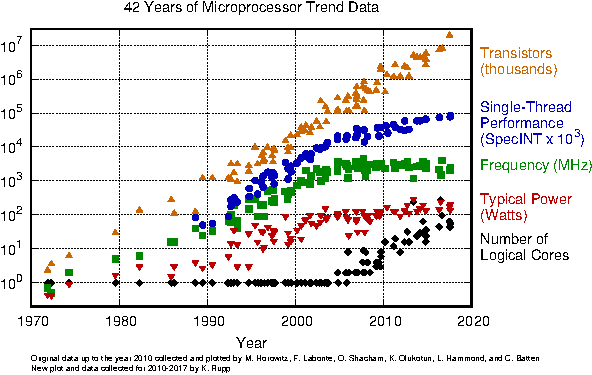
\includegraphics[scale=1.5]{42-years-processor-trend.pdf}
 \caption{42 years of microprocessor trend data \citep{42years}.}
 \label{fig:42years}
\end{figure}

\begin{subsection}{\textit{Speedup}}
	One way to measure the time reduction of a parallel implementation
	is through the concept of speedup. 

\begin{definition}
	Let $T_1$ be the time of a sequential algorithm and $T_n$ the time
	of this same algorithm parallelized with $n$ cores. Then the
	\textbf{speedup} $S_n$ is given by:
    $$ S_n = \frac{T_1}{T_n} $$
\end{definition}

%    Uma maneira de medir o ganho de tempo em uma implementação paralela
%de um algoritmo é através no conceito de \textit{speedup}. Sejam $T_1$
%o tempo do algoritmo sequencial e $T_n$ o tempo desse algoritmo paralelizado
%    com $n$ núcleos de processamento. Então o \textit{speedup} $S_n$
%é dado por:

\end{subsection}


\begin{subsection}{Flynn Taxonomy}
%	Mesmo com a evolução dos processadores \textit{multicore} e
%\textit{manycore}, estas não são as únicas arquiteturas disponíveis para
%realizar computação paralela. Michael J. Flynn \citep{pacheco:2011} definiu
%uma taxonomia das arquiteturas, mas vale destaque para duas delas:

Even with the evolution of multicore and manycore processors, those are not the
only architectures available for parallel computing.  Michael J. Flynn
\citep{pacheco:2011} defined a taxonomy of architectures, however, two of them
must be highlighted:

\begin{enumerate}
	\item \textbf{SIMD} - \textit{Single Instruction, Multiple Data}. Those are
	vectorial processors that allow a single operation to be executed
	simultaneously in every element of a vector. Some examples are the Intel SSE
	instruction set, and also the \textit{Graphics Processing Units} (GPU) although
	this last one is not considered a pure SIMD architecture.

    \item \textbf{MIMD} - \textit{Multiple Instruction, Multiple Data}. Those
are the completely independent multicore systems, capable of
executing tasks asynchronously. Here we find both shared memory and distributed memory architectures.

\end{enumerate}
\end{subsection}

\begin{subsection}{Parallel Programming in Shared Memory}
	One way of doing Parallel Computing is through a shared memory
	behind the cores or processors. Here, a shared memory is connected
	through a bus to all processors, allowing read and write of data.
	To avoid concurrency problems, both locking and synchronization mechanisms
	are required.

%	Uma maneira de permitir Computação Paralela é através de
%uma memória compartilhada. Aqui vários processadores ou núcleos
%são ligados através de um barramento a uma memória compartilhada entre
%todos os processadores, que permite leitura e escrita de dados.
%Para evitar problemas de concorrência, são necessários mecanismos de
%travas e sincronização.

	Here, most resources are provided by the Operating System (OS),
	and therefore a brief explanation is required about its abstractions.

%	 Aqui, muitos dos recursos para sincronização são fornecidos pelo
%Sistema Operacional (OS), e portanto é necessário explicar um pouco
%das abstrações que ele fornece.

\begin{subsubsection}{Process and Threads}

	Before the existence of multicore processors, a processor
	could only execute a program at a time. With this fact in
	mind, Operating System developers created a series of abstractions
	so that the user could have the illusion that several programs were
	executing simultaneously. Although this is not true anymore, this
	is the primary fact between the concept of Process and Threads.

%	Antigamente, os processadores eram capazes de executar apenas
%um programa por vez. Com isto em mente, os desenvolvedores
%de Sistemas Operacionais criaram uma série de abstrações para que fosse
%possível dar a ilusão ao usuário que vários programas estavam executando
%ao mesmo tempo. Embora isso não seja mais um fato, já que hoje os processadores
%são capazes de executar vários fluxos de execução simultaneamente, essa
%é a principal motivação do conceito de Processos e \textit{Threads}.

A \textit{process} is an abstraction provided by the Operating System which
gives to the program the illusion that it has the processor's monopoly
\citep{love:2005}. Each process has its own memory region, and sharing
information between processes must be done through Interprocess Communication
(IPC). One example of such is the \texttt{shmget} call, from \texttt{System V},
in which Linux still supports \citep{shmget}, or through a Pipe \citep{pipe}.

%	Um \textit{Processo} é um modelo de abstração do Sistema Operacional que
%dá a um programa a ilusão de que ele tem o monopólio do processador
%\citep{love:2005}. Cada processo tem a sua região de memória privada por
%padrão, e para que processos possam compartilhar memória, isso deve ser 
%explicitado no programa. Um exemplo onde isso pode ser feito é através das
%chamadas \texttt{shmget} do extinto \texttt{System V}, mas cujo o Linux ainda
%oferece suporte \citep{shmget}.

Each process contains at least one execution flow, and each execution
flow is called a \textit{thread}. Each thread inside a process
shares memory with every other thread from the same process, except
for its stack and the Thread Local Storage (TLS) region, which turns
the development of communication mechanisms easier.

When parallelizing a program, the programmer must choose between using threads
or processes. By selecting threads, the programmer will have the advantage of
having access to global data structures and therefore an easy communication
between the threads. However, race conditions must be solved individually,
which may become cumbersome when the software is really large. By selecting to
parallelize through processes, most race conditions may fade away, but then the
issue revolves around find \textit{what} must be shared and how to do an
efficient communication between processes, as IPC can be slow.

Unix processes are created through a system call named \textit{fork}. On
Linux, forking will clone the current process into another, and copy
the pages only when modified, a process named Copy on Write (CoW). This
may turn into an additional overhead when processes are chosen instead
of threads \citep{abbas_cow}.

%Cada processo contém pelo menos um fluxo de execução, e cada fluxo de
%execução é chamado de \textit{thread}. Cada \textit{thread} dentro
%de um processo compartilha memória com as demais \textit{threads}
%do processo, facilitando assim o desenvolvimento de mecanismos de
%comunicação através de uma memória compartilhada.

\end{subsubsection}

\begin{subsubsection}{Sincronization Mechanisms}

An Operating System usually provides synchronization mechanisms to control
several threads of a process or even several processes. These mechanisms are
often implemented with the help of hardware resources, however, they can also
be implemented purely in software.

%	Seja através de auxílio do \textit{hardware}, ou com algoritmos
%puramente implementados em \textit{software}, o Sistema Operacional
%costuma fornecer mecanismos de sincronização para coordenar as várias
%\textit{threads} de um processo, ou até mesmo vários processos.

One of such mechanisms are \textit{Semaphores} \citep{dijkstra1965}.  A
semaphore is a counter which can assume non-negative integer values with
two atomic operations: \texttt{P} to decrement it, or \texttt{V} to
increment it. When the semaphore reaches 0, the next thread that will try
to decrement it will be blocked. Its execution will only be resumed when
another thread increments the semaphore.

%\citep{dijkstra1965}. Um semáforo nada mais é que um contador que assume
%valores não negativos com duas operações atômicas: \texttt{P} para
%decrementá-lo, e \texttt{V} para incrementá-lo. Quando o semáforo atinge o
%valor 0, a \textit{thread} que em sequência tentar decrementá-lo será bloqueada. A
%sua execução apenas será retomada quando o semáforo for novamente incrementado
%por outra \textit{thread} \citep{semaphore}.

Semaphores can also be used to solve the critical section problem, which is
when only one thread must be executing a section of the code at a time.
However, such a problem is often solved using \textit{mutexes}.

%    Semáforos também podem ser utilizados para resolver o problema da
%seção crítica, que é uma seção de código que apenas uma \textit{thread}
%deve poder executar por vez, embora seja mais comum a utilização
%de \textit{Mutexes}.

Mutexes are a structure that ensures the mutual exclusion of a code region, as
illustrated in Figure \ref{fig:mutex}. In this figure, three threads are
started executing a function named $f$, but only one can execute the critical
section at the time.

%\textit{Mutexes} nada mais são que uma estrutura que garante a exclusão
%mútua de uma região, conforme ilustrado na Figura \ref{fig:mutex}. Nessa
%figura, três \textit{threads} são iniciadas executando a função $f$, mas
%apenas uma pode executar a seção crítica.

When a mutex is locked, every other thread that tries to access
the critical section will be blocked by the Operating System,
ensuring that only one thread will be executing this section.
Every blocked thread will be unlocked when the thread that
locked the mutex unlocks it. This is the main difference between
a mutex and a binary semaphore.

%    Quando o \textit{mutex} \texttt{lock} é travado,
%todas as outras \textit{threads} que tentarem acessar a seção crítica
%serão bloqueadas pelo Sistema Operacional, garantindo assim que apenas
%uma \textit{thread} esteja executando a seção crítica.
%As \textit{threads} bloqueadas somente voltarão a executar quando o
%    \textit{mutex} for desbloqueado pela \textit{thread} que o travou.
\begin{figure}
      \begin{lstlisting}[
        language=pseudocode,
        style=pseudocode,
        style=wider,
        functions={},
        specialidentifiers={extern, call, async, mutex_t},
      ]
        extern function mutex_lock, mutex_unlock;
        mutex_t lock;

        async function f()
            mutex_lock(lock);
                // Critical section
            mutex_unlock(lock);
        end

        function main()
            for i=1, 3 do
                call f;
            done
        end
      \end{lstlisting}
      \caption{A mutex usage illustration.}
      \label{fig:mutex}
\end{figure}

Another useful synchronization mechanism is the barriers. A barrier is a point
in the program where once a thread executes it, it will be blocked until every
other thread reach the same point, as illustrated in Figure \ref{fig:barrier}.
This is very useful to avoid that one thread advances in the execution of a
code when it should be waiting for the result of some computation by another
thread. Barriers also receive an integer specifying how many threads should
reach the barrier for every thread to be allowed to continue with its
execution.

%Outro mecanismo de sincronização muito útil são as Barreiras. Uma barreira
%é um ponto no programa onde, assim que a \textit{thread} o executar, ela
%será bloqueada até que todas as \textit{threads} cheguem ao mesmo ponto, como
%ilustrado na Figura \ref{fig:barrier}.
%Isso é bastante útil para evitar que uma \textit{thread} avance na execução
%do código enquanto ela deveria estar aguardando o resultado da computação
%de outras \textit{threads}. As barrerias também costumam receber um parâmetro
%de inicialização indicando quantas \textit{threads} precisam atingir a
%barreira para que todas as \textit{threads} que a atingiu sejam desbloqueadas.

\begin{figure}[ht]
 \centering
 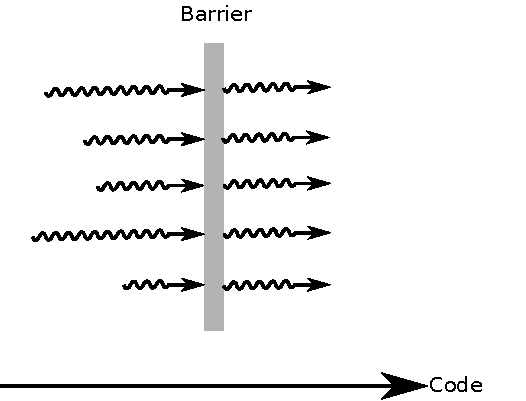
\includegraphics[scale=1.0]{barrier.pdf}
 \caption{A barrier usage illustration.}
 \label{fig:barrier}
\end{figure}

Except for semaphores, every mechanism mentioned above is implemented in the
\textit{pthread} library. Semaphores, on the other hand, are available in Linux
through the \texttt{semaphore.h} interface.

%Por fim, exceto os semáforos, todos esses mecanismos mencionados acima são
%implementados na biblioteca \texttt{Pthread}. Já os semáforos estão disponíveis
%no Linux através da interface \texttt{semaphore.h}.

\end{subsubsection}

\begin{section}{Power and Energy}\label{sec:power}

When we want to measure how much energy a computer is consuming, there are
sensors to measure the \textit{Instantaneous Power}. However, power $P$ is
defined as the time rate of energy transferred \citep{young2006sears}.
Therefore, to compute energy measuring the power consumption of a system: $$P =
\frac{dE}{dt} \quad \Rightarrow \quad E = \int_{0}^{t'} P(t)dt$$ where $t'$ is
the elapsed time of the experiment. However, we can only measure information of
the sensor in discrete time, and not continuously.  Therefore we can
approximate this integral by using two Riemann sums.

Assume that we collected $n$ measurements of the sensor at times
$t_1, t_2, \cdots, t_n$ with a distance of $\Delta t$ from each other.
Now, given two measured points at time
$t_i$ and $t_{i+1}$, we define a \textit{minimum} and \textit{maximum} $m_i$ and $M_i$
such that:
$$m_i = \min\{P(t_i), P(t_{i+1})\} \quad \text{ and } \quad M_i = \max\{P(t_i), P(t_{i+1})\}$$
Then, assuming that for every $x \in [t_i, t_{i+1}]$ we have
$$m_i \leq P(x) \leq M_i$$
this means that:
$$\sum_{i=1}^{n-1} m_i\Delta t \leq E \leq \sum_{i=1}^{n-1} M_i\Delta t$$
Which can give us a way to measure the \textit{error} of our integration
process just by computing $\sum_{i=1}^{n-1} M_i\Delta t -
\sum_{i=1}^{n-1} m_i\Delta t = \epsilon$. This can also capture the error of the sensor
itself by representing the real value as between a range of two values, and
the lower bound on $m_i$ and the upper bound in $M_i$.

\end{section}

%\begin{subsubsection}{O Problema do Produtor-Consumidor}
%    Uma estrutura de dados muito útil em computação paralela
%é uma fila completamente \textit{Thread-safe}, ou seja,
%que várias \textit{threads} possam inserir e remover dados dessa
%fila simultaneamente sem o risco de perda de dados. Essa fila
%pode ser usada na comunicação entre as \textit{threads}, por
%exemplo: uma insere trabalho na fila, outra retira trabalho da
%fila. Isso permite com que \textit{pipelines}, ou escalonamento
%dinâmico de trabalho sejam implementados.
%
%Para implementar essa fila, são necessários dois semáforos e um
%\textit{mutex}. Um semáforo deve ser inicializado com o tamanho máximo
%da fila, e na inserção de um dado, esse semáforo deve ser decrementado
%para que, quando a fila estiver cheia, as \textit{threads} que tentarem
%inserir nela sejam bloqueadas. O outro semáforo deve ser iniciado com
%0, indicando que a fila está vazia, e incrementado quando um item for
%inserido na fila. Esse semáforo tem a finalidade de
%bloquear as \textit{threads} que tentarem remover elementos dessa
%fila quando ela estiver vazia. Assim que dados forem inseridos ou removidos
%da fila, as \textit{threads} são devidamente ``despertadas''. Isso evita gasto
%desnecessário de ciclos de processamento por não utilizar uma técnica
%chamada \textit{espera ocupada}. Por fim, um \textit{Mutex} deve ser
%utilizado para evitar problemas de concorrência ao incrementar e
%decrementar os apontadores de inicio e fim da fila.
%Uma implementação
%é apresentada na Figura \ref{fig:prod_consumer}.
%\begin{figure}
%      \begin{lstlisting}[
%        language=pseudocode,
%        style=pseudocode,
%        style=wider,
%        functions={},
%        specialidentifiers={extern, call, async, int, class, mod, semaphore_t, mutex_t},
%      ]
%        class Fifo
%            int buffer[];
%            int size;
%            int head, tail;
%            semaphore_t full, empty;
%            mutex_t lock
%
%            function init(n)
%                buffer = allocate_memory(n);
%                head, tail = 0;
%                sem_init(empty, n);
%                sem_init(full, 0);
%                mutex_init(lock);
%                size = n;
%            end
%
%            function push(element)
%                sem_p(empty);
%                mutex_lock(lock);
%                buffer[head] = element;
%                head = head + 1 mod size;
%                mutex_unlock(lock);
%                sem_v(full);
%            end
%
%            function pop()
%                sem_p(full);
%                mutex_lock(lock);
%                ret = buffer[tail];
%                tail = tail + 1 mod size;
%                mutex_unlock(lock);
%                sem_v(empty)
%
%                return ret;
%            end
%        end 
%
%      \end{lstlisting}
%      \caption{Uma implementação do Produtor-Consumidor.}
%      \label{fig:prod_consumer}
%\end{figure}
%
%\end{subsubsection}

\end{subsection}

\end{section}

% Vamos definir alguns comandos auxiliares para facilitar.

% "textbackslash" é muito comprido.
\newcommand{\sla}{\textbackslash}

% Vamos escrever comandos (como "make" ou "itemize") com formatação especial.
\newcommand{\cmd}[1]{\textsf{#1}}

% Idem para packages; aqui estamos usando a mesma formatação de \cmd,
% mas poderíamos escolher outra.
\newcommand{\pkg}[1]{\textsf{#1}}

% A maioria dos comandos LaTeX começa com "\"; vamos criar um
% comando que já coloca essa barra e formata com "\cmd".
\newcommand{\ltxcmd}[1]{\cmd{\sla{}#1}}

\chapter{Trabalhos Relacionados}
\label{chap:related_works}

Nesta seção é discutido trabalhos relacionados a paralelização de compiladores.
É importante mencionar que boa parte das pesquisa relacionada a paralelismo
em compiladores é destinada a compiladores que paralelizam. Há basicamente
duas áreas de estudo relacionadas a paralelização de compiladores, são
elas: análise de texto em paralelo, e análise de fluxo de dados em paralelo.
Estes trabalhos também são abordados nessa seção, em ordem cronológica.

Dos algoritmos apresentados na Seção \ref{chap:fundamentacao}, o algoritmo
Recursivo Descendente é o mais simples deles. \cite{Lincoln:1970:PPT:987475.987478}
propôs uma maneira de paralelizar a análise léxica de um compilador
Fortran simplesmente quebrando o código fonte em partes, mapeando as
informações de final de
linha e a posição de cada caractere, e realizando o processamento
através de operações em APL.
Posteriormente, \cite{Krohn:1975:PAC:390015.808414} estendeu o trabalho
anterior, propondo uma maneira de realizar a análise sintática, a
tradução para a AST, e a geração
de código utilizando os registradores vetoriais do supercomputador
STAR-100. Ambos os artigos também não apresentam nenhuma
análise assintótica para os algoritmos propostos, e também não apresentam
experimentos. 

Posteriormente, \cite{Mickunas:1978:PCM:800127.804105} propôs uma
paralelização do algoritmo LR($0$). Sua ideia consiste em quebrar
arbitrariamente a entrada em vários segmentos e executar um analisador em paralelo
em cada um destes segmentos. Estes analisadores (exceto o primeiro,
que executa no inicio da entrada) são modificados na tentativa de
evitar conflitos, uma vez que modificar a ordem de inicio da análise
pode impossibilitar distinguir entre o prefixo e o sufixo de uma fase.
Quando um conflito é detectado, o analisador envia a sequência de
\textit{tokens} lido até então ao analisador à sua esquerda,
retorna ao estado inicial, e reinicia a sua análise.
No termino da análise, cada analisador envia o resultado para o analisador
a sua esquerda, acumulando o resultando no primeiro analisador.
Os autores não mostraram experimentos ou
análise assintótica do algoritmo proposto. \cite{Pennello:1978:FMA:512760.512786}
implementou essa estratégia em um compilador Pascal, mas seus experimentos foram
realizados em um computador paralelo simulado.

\cite{vandevoorde1988parallel} paralelizou o \textit{Titan C compiler}, um compilador
C escrito em Modula-2. Sua implementação utiliza um analisador léxico executando
paralelamente ao analisador sintático, e os \textit{tokens} são alimentados
através de um \textit{pipeline}. Ele também propôs uma paralelização de um
analisador sintático recursivo descendente, executando novas \textit{threads}
para cada expressão da gramática após a sequência de declarações do programa,
usando como premissa que qualquer declaração de funções do programa está no
cabeçalho do
arquivo. Essa estratégia de granularidade fina necessitou a implementação de
uma maneira de controlar o paralelismo, onde foi utilizado o conceito de
WorkCrews \citep{vandevoorde1988workcrews}, limitando o número máximo de
\textit{threads} em execução simultânea. O autor relata um ganho de 10\% no
uso do \textit{pipeline} entre o analisador léxico e sintático, e um
\textit{speedup} de até $3.1\times$ utilizando 5 processadores MicroVax II em
memória compartilhada.  Entretanto, o compilador não possui estágios de
otimização e o autor não discute como paralelizar um otimizador.

De maneira similar, \cite{wortman1992} construiu um compilador de Modula-2+
paralelo. A estratégia proposta é utilizar um analisador léxico capaz de
encontrar funções no código fonte e prosseguir com a compilação em paralelo
nesse nível, gerando uma tarefa para cada função. Para solucionar problemas
relacionados a chamada de funções e
acesso a símbolos ainda não definidos, o autor propõe o uso de
uma lógica ternária na tabela de símbolos, especificando um estado
``\textit{Doesn't know yet}'' (Ainda não visto), e propõe três estratégias para
implementar essa funcionalidade. Em seguida, o autor propõe o uso de
um número fixo de \textit{threads} trabalhadoras, e o uso de uma fila de
prioridade produtor consumidor, onde as \textit{threads} deverão retirar o trabalho.
O uso de uma fila de prioridade permite com que as funções mais longas sejam
processadas primeiro. Os experimentos conduzidos pelo autor mostraram
\textit{speedups} variando de $1.5\times$ até $6\times$ utilizando 8
processadores MicroVAX II em memória compartilhada.

Deve ser destacado que os artigos até então não abordam questões relacionadas
a otimização de código. Isso porque os compiladores até então haviam poucos
passos de otimização, o que implicava em pouco tempo necessário para fazê-la.
Mesmo assim, alguns pesquisadores dedicaram-se a estudar esses passos.
\cite{Lee1994} estudou maneiras de explorar paralelismo na análise de controle
de fluxo. Os autores argumentam que os compiladores otimizadores gastam a maior
parte do tempo realizando tais análises, principalmente nas otimizações Inter
Procedurais. A análise se concentra em algoritmos que usam o grafo de controle
de fluxo como entrada, sendo assim os autores propõem uma heurística de aglutinação
para particionar tal grafo em regiões conexas e adjacentes de tamanho não maior
que um certo inteiro $s$, já que o
problema geral é NP-difícil. Os autores experimentam sua implementação utilizando
8 processadores do computador iPSC/2 em memória distribuída, e 
relatam \textit{speedups} variando de
$2.8 \times$ até $6.5\times$. Os autores relataram que o \textit{speedup} foi
limitado pela característica dos programas no teste: os arquivos consistiam
de várias funções pequenas, o que normalmente é considerado uma boa prática de
programação. Uma outra forma de explorar o paralelismo nessas estruturas
foi proposta por \cite{kramer1994combining}.

Após estes resultados, houve um aparente hiato nas pesquisas relacionadas a
compilação em paralelo. Uma causa possível é o fato de um compilador ser
um programa muito complexo, e os processadores até então ainda serem, em sua grande
maioria, sequenciais. Uma década depois, houve uma explosão de processadores
paralelos e poder computacional como um todo, como apresentado na Seção
\ref{sec:parallel_comp}, o que levou a empresas propor soluções mais eficazes para
gerar código mais eficiente. Embora não diretamente relacionado a compiladores paralelos,
algumas estruturas propostas acabam tocando nesse tópico.

\cite{whoprgoogle} propôs uma alteração no
compilador GCC com a finalidade
de possibilitar otimizações no programa como um todo. A alteração consiste
em construir um grafo de chamadas de função em relação a todo o programa,
ao contrário do modelo clássico, em que cada módulo é compilado independentemente.
Esse processo consiste em três etapas:
\begin{enumerate}
    \item \textit{Local Generation } (LGEN). Cada função do programa é compilado
        na Linguagem Intermediária, em conjunto com o grafo de chamadas de função.
        Esse estágio pode executar em paralelo.

    \item \textit{Whole Program Analysis} (WPA). O grafo de chamadas de função global
        é construído, e é decidido quais otimizações efetuar. Essa estágio
        deve ser executado sequencialmente.

    \item \textit{Local Transformations} (LTRANS). Todas as decisões aplicadas na
        etapa 2 são implementadas localmente, e o código objeto final é gerado.
        Esse estágio pode executar em paralelo.
\end{enumerate}

A Figura \ref{fig:whopr_build} retrata este processo. Essa proposta foi implementada
no GCC \citep{glek2010optimizing} com o nome de
\textit{Link Time Optimization} (LTO). A granularidade
escolhida na etapa LGEN foi paralelismo por arquivo, já na LTRANS a granularidade
escolhida são partições do arquivo objeto, e por consequência é possível otimizar
funções de um arquivo em paralelo. Os autores testaram essa implementação com o
código fonte do Mozilla Firefox e do GCC, e relataram que o GCC construiu
binários menores e mais rápidos. Os autores relataram que esse processo tornou
o processo de autocompilação do GCC duas vezes mais lenta,
mas que também houve um ganho de 20 minutos na compilação do Firefox. Em todos os
casos relatados, os passos de otimização Intra Procedural consumiu mais tempo.
\cite{livska2014optimizing} completa a análise dessa funcionalidade.
Um dos problemas que surgem é o uso elevado de memória para carregar o grafo de
chamadas de função global, necessário na fase WPA, chega a 12Gb na compilação do
Chromium e 15Gb na compilação do Kernel Linux. A maior crítica a esse processo
era o tempo necessário para recompilar todo o programa quando uma simples alteração
era efetuada em um único arquivo, inviabilizando um desenvolvimento incremental.

\begin{figure}
\tikzstyle{block} = [rectangle, draw, fill=white,
    text width=6em, text centered, rounded corners, node distance=3cm, auto, minimum height=2em]
\tikzstyle{line} = [draw, -latex]
\tikzstyle{cloud} = [draw, ellipse,fill=white, node distance=2cm,
    minimum height=2em]
\begin{center}
\scalebox{0.7}{
\begin{tikzpicture}[node distance = 3cm, auto]
    % Place nodes
    \node [block]                         (make)   {Makefile};
    \coordinate[below of=make]            (c);
    \node [block, left of=c]              (fonte1) {fonte1.c};
    \node [block, right of=fonte1]        (fonte2) {fonte2.cpp};
    \node [block, right of=fonte2]        (fonte3) {fonte3.f90};

    \node [block, below of=fonte1]        (gcc)      {gcc};
    \node [block, below of=fonte2]        (g++)      {g++};
    \node [block, below of=fonte3]        (gfortran) {gfortran};

    \node [block, below of=gcc]           (objeto1) {lto\_obj1.o};
    \node [block, below of=g++]           (objeto2) {lto\_obj2.o};
    \node [block, below of=gfortran]      (objeto3) {lto\_obj3.o};

    \node [block, below of=objeto2]       (gcc_lto) {gcc\_lto1};

    \node [block, below of=gcc_lto]       (gcc_wpa) {gcc\_wpa};
    \coordinate[below of=gcc_wpa]            (c2);

    \node [block, left of=c2]            (gcc_ltrans1) {gcc\_ltrans};
    \node [block, right of=gcc_ltrans1]   (gcc_ltrans2) {gcc\_ltrans};
    \node [block, right of=gcc_ltrans2]   (gcc_ltrans3) {gcc\_ltrans};

    \node [block, below of=gcc_ltrans1]   (obj1) {obj1.o};
    \node [block, below of=gcc_ltrans2]   (obj2) {obj2.o};
    \node [block, below of=gcc_ltrans3]   (obj3) {obj3.o};

    \node [block, below of=obj2]   (ld) {LD};

	\node [block, below of=ld]   (bin) {Executável};

    % Draw edges
    \draw[->]    ([xshift=-0.7em] make.south)   -- (fonte1.north);
    \draw[->]    (make.south)   -- (fonte2.north);
    \draw[->]    ([xshift=+0.7em] make.south)   -- (fonte3.north);

    \draw[->]    (fonte1.south)   -- (gcc.north);
    \draw[->]    (fonte2.south)   -- (g++.north);
    \draw[->]    (fonte3.south)   -- (gfortran.north);

    \draw[->]    (gcc.south)   -- (objeto1.north);
    \draw[->]    (g++.south)   -- (objeto2.north);
    \draw[->]    (gfortran.south)   -- (objeto3.north);

    \draw[->]    (objeto1.south)   -- ([xshift=-0.7em]gcc_lto.north);
    \draw[->]    (objeto2.south)   -- (gcc_lto.north);
    \draw[->]    (objeto3.south)   -- ([xshift=+0.7em]gcc_lto.north);

    \draw[->]    (gcc_lto.south)   -- (gcc_wpa.north);

    \draw[->]    (gcc_wpa.south)   -- (gcc_ltrans1.north);
    \draw[->]    (gcc_wpa.south)   -- (gcc_ltrans2.north);
    \draw[->]    (gcc_wpa.south)   -- (gcc_ltrans3.north);

    \draw[->]    (gcc_ltrans1.south)   -- (obj1.north);
    \draw[->]    (gcc_ltrans2.south)   -- (obj2.north);
    \draw[->]    (gcc_ltrans3.south)   -- (obj3.north);

    \draw[->]    (obj1.south)   -- ([xshift=-0.7em]ld.north);
    \draw[->]    (obj2.south)   -- (ld.north);
    \draw[->]    (obj3.south)   -- ([xshift=+0.7em]ld.north);

	\draw[->]    (ld.south)   -- (bin.north);


\end{tikzpicture}
}
\end{center}
\caption{Compilação de um programa utilizando WHOPR.}
\label{fig:whopr_build}
\end{figure}


Considerando o alto uso de memória e tempo de compilação nos casos relatados
acima, \cite{Johnson:2017:TSI:3049832.3049845} propôs o ThinLTO. A ideia é
considerar apenas parte do grafo global a cada vez, evitando carregá-lo
completamente na memória; e postergar ao máximo aplicar as otimizações possíveis,
realizando apenas análises de maneira sequencial, e aplicando-as no 
\textit{backend} em paralelo.
Os autores relataram um \textit{speedup} de até $15\times$ quando comparado a
implementação do LTO original do Clang, e até $4\times$ quando comparado a
implementação do LTO do GCC. Os autores também relataram uma diminuição considerável
no consumo de memória quando comparado ao LTO do GCC: Redução de 2.9Gb para 1Gb
na compilação do Clang, 10.8Gb para 1.0Gb no Chromium, e permitiu melhores otimizações no
\textit{Ad Delivery} da Google, enquanto a implementação do LTO no GCC
abortava a compilação após consumir mais de 25Gb de memória. O desempenho dos
binários gerados também foi similar, inclusive onde o LTO original gerava
binários mais lentos que o processo clássico de compilação. O tempo de compilação
também melhorou significativamente quando comparado ao LTO original,
mas permaneceu pior em todos os casos quando comparado ao processo clássico de
compilação.

Houve também um renascimento nas pesquisas de análise sintática em paralelo.
\cite{Barenghi:2015:PPM:2839536.2840146} encontrou uma maneira de explorar
a propriedade de Análise Local em Gramáticas com Precedência de Operadores.
Isso permitiu a construção de um gerador de analisadores sintáticos
PAPAGENO (\textit{Parallel Parser Generator}). Para isto, a gramática a
ser utilizada nesse analisador precisa ser convertida para uma Gramática
com Precedência de Operadores, conforme discutido e exemplificado pelos
autores. Testes empíricos foram efetuados implementando um analisador
JSON e outro analisador para a linguagem Lua. Em um Opteron 8378 (16 núcleos),
os autores atingiram um \textit{speedup} de até $5.3\times$ no análisador JSON
em arquivos grandes, e pouco mais de $4\times$ no analisador Lua. O algoritmo
paralelo foi comparado com os gerados pelo analisador sintático \textit{Bison},
que apenas gera código sequencial.



\chapter{Proposta de Trabalho}
\label{chap:proposta}

Neste capítulo é apresentado um plano de trabalho que será elaborado
durante o período após a qualificação, e resultados esperados.
Este trabalho tem o objetivo de trazer duas contribuições:
\begin{enumerate}
    \item Uma opção no compilador GCC para que ele seja
capaz de compilar um único arquivo em paralelo sem utilizar a
estrutura do LTO. Isso é útil para desenvolvedores que trabalham
com grandes softwares iterativamente, pois deve minimizar
gargalos gerados por arquivos grandes e cobrir os casos onde o LTO gera
binário menos eficientes que o processo clássico de compilação, fornecendo assim
uma alternativa ao LTO.
Essa tese se concentra em paralelizar os passos de otimização Intra Procedural
a nível de funções, ou seja, duas análises executarão em paralelo em funções
distintas, evitando adentrar em paralelizar a análise de fluxo de dados.

    \item Uma revisão sobre o que pode ser feito para acelerar o
processo clássico de compilação em máquinas \textit{manycore}, através
de paralelismo, e quais problemas devem ser atacados em trabalhos futuros.
Espera-se utilizar os resultados do item 1.
\end{enumerate}
O primeiro item será enviada ao GCC como como uma contribuição
ao \textit{software} livre. O projeto de paralelização foi submetido para o GSoC 2019,
conforme o Apêndice \ref{ap:gsoc}.


\section{Paralelização do GCC com \textit{threads}}

Nesta subseção é apresentado o estado atual do projeto de paralelização
do GCC com \textit{threads}. O GCC foi escolhido como candidato para
paralelização pois a comunidade demonstrou grande interesse no projeto,
conforme discutido na Seção \ref{cap:introducao}, e o autor desta tese ter alguma
familiaridade com o projeto, já tendo contribuído com este. Sendo assim,
utilizar outro compilador como o Clang para implementar o projeto demandaria
estudos sobre a estrutura do projeto e convencer parte da comunidade de que
o trabalho trás alguma vantagem ao projeto. Por outro lado, implementar um
novo compilador não é uma alternativa viável dado que um dos maiores gargalos
na compilação é o otimizador, peça que não seria possível implementar em
dois anos algo tão poderoso como o GCC ou o Clang.

Como atestado por \cite{PR84402}, há um gargalo de paralelismo dentro do
próprio GCC por conta de arquivos grandes, e \cite{mailgcc} também
relatou um gargalo em outro projeto interno. Uma das soluções para este
problema é melhorar o paralelismo dentro do GCC, tornando possível fazer
com que a compilação utilize mais núcleos de processamento.
Nesta discussão, foi proposto uma maneira de visualizar o problema de
paralelismo através de um gráfico gerado por dados de um GNU Make modificado.
Como a alteração no Make é razoavelmente complicada e o \textit{script} proposto
havia sérios problemas de estabilidade, foi desenvolvido uma outra maneira
de replicar os resultados.

Como desenvolvido e publicado por \cite{gcctimer}, a ferramenta aqui proposta
é capaz de coletar e exibir dados referente ao tempo de compilação
de cada arquivo no GCC, incluindo os testes gerados pelo GNU Autotools.
A ferramenta funciona da seguinte forma: há um programa escrito em C chamado
\texttt{cc\_wrapper} que encapsula o compilador C e C++ do ambiente, no caso o 
GCC e o G++. O caminho para estes compiladores são passados como um parâmetro
da compilação do \texttt{cc\_wrapper} de maneira que os binários gerados os
simulem. Em seguida o programa abre um novo processo através do \texttt{fork()},
chamando o GCC/G++ com os parâmetros passados a ele sem alterações. O processo
inicia a coleta do tempo, busca pelo nome do arquivo objeto a ser gerado, e
aguarda o GCC chamado terminar. Essa busca foi codificada de maneira a ser
muito eficiente, tento um pior caso $O(n)$ com uma constante muito baixa,
onde $n$ é o número de parâmetros passados ao GCC. Em seguida, o programa
escreve o tempo de início, tempo de fim, e o nome do arquivo em um arquivo
de texto. Houve cautela para que não haja mistura de linhas
no arquivo por razão de escrita simultânea no arquivo. Há também um \textit{script}
em \textit{Bash} para reproduzir os resultados facilmente.

Em seguida, foi codificado um programa em \textit{Python} para análise dos
resultados. Esse programa é responsável por gerar os gráficos conforme
mostrado na Figura \ref{fig:analysis_classical}. Em um dos eixos há o
tempo de execução, no outro há
o trabalho do Makefile. Para construir o gráfico, é considerado que
dois intervalos que se interseccionam apenas podem ser executados em
trabalhos distintos do Make, sendo assim é utilizado a técnica
de coloração em grafos de intervalos, que pode ser resolvido otimamente
em $O(n \log p)$, onde $n$ é o número de arquivos e $p$ é o número de
cores, embora o algoritmo
implementado seja $O(np)$.

\subsection{Inverstigação do Tempo Consumido na Compilação}

Uma investigação foi conduzida com a finalidade de encontrar o gargalo
principal no processo de compilação do GCC. Todos os testes efetuados foram
executados em um computador com um AMD Opteron 6376 (64 núcleos) executando
o Debian 9.

Novamente na Figura \ref{fig:analysis_classical}, é possível notar dois
itens, independente da quantidade de execuções do experimento:

\begin{itemize}
    \item A existência de arquivos como o \texttt{gimple-match.c}, que
        geram um gargalo no paralelismo do GCC.

    \item Várias etapas sequênciais executadas pelo GNU Autoconf.
\end{itemize}

O arquivo \texttt{gimple-match.c} é gerado automaticamente compilando
o arquivo \texttt{match.pd} para C. Na versão 9.0.1 do GCC, o arquivo
gerado contém exatamente 99329 linhas de código. Espera-se que o tempo
de compilação do \texttt{gimple-match.c} diminua, em conjunto com o tempo
total de compilação, ao paralelizar o GCC com \textit{threads}.

Analisando o tempo necessário para compilar o arquivo \texttt{gimple-match.c},
foi possível notar que:
\begin{itemize}
    \item São necessários em média 76 segundos para compilar tal arquivo.

    \item 91\% desse tempo (69 segundos) são utilizados na etapa de otimização
        e geração de código final.

    \item 8\% desse tempo (6 segundos) são utilizados na etapa de análise léxica
        e sintática.

    \item O outro 1\% está distribuído em diversas partes do compilador.
\end{itemize}
Todos estes dados foram obtidos autocompilando o GCC 9.0.1, e utilizando a
ferramenta de \textit{profiling} incorporada
no GCC através das flags \texttt{-ftime-report} \texttt{-ftime-report-details}.

Como as otimizações do GCC são divididas em IPA, GIMPLE e RTL, é necessário
executar uma granularidade mais fina na análise. Com uma simples alteração
no GCC, foi possível separar a etapa IPA das demais. Bastou embrulhar as funções
\texttt{ipa\_passes()} e \texttt{expand\_all\_functions()} com duas\textit{timevars}
distintas. Assim, os dados são:
\begin{itemize}
    \item 75\% do tempo total de compilação (57s) é gasto nos passos de otimização
        Intra Procedural e geração de código.

    \item 11\% do tempo total de compilação (11s) é gasto para realizar as IPA.
\end{itemize}
Sendo assim, o principal candidato a paralelização é a função \texttt{expand\_all\_functions()}.
Entretanto, para realizar tal paralelização, será necessário documentar e remover diversas
variáveis globais do GCC de maneira que seja possível realizar paralelismo com \textit{threads}.

\subsection{Análise do \textit{Speedup} Máximo}

Conforme analisado acima, se paralelizarmos as etapas de otimização Intra
Procedural e Geração de Código, é possível paralelizar 75\% do tempo total.
Sendo assim, seja $p$ o número de processadores utilizados. Assumindo
\textit{speedup} linear, o ganho máximo será:

$$ T_p = \frac{1}{4} T_1 + \frac{3}{4p}T_1 = \frac{1}{4} \left( 1 + \frac{3}{p}
\right)T_1 $$ Sendo assim, o \textit{speedup} máximo por arquivo será: $$
\lim_{p \rightarrow +\infty} \frac{T_1}{T_p} = \lim_{p \rightarrow +\infty}
\frac{T_1}{\frac{1}{4} \left( 1 + \frac{3}{p} \right)T_1} = \lim_{p \rightarrow
+\infty} \frac{4}{1 + \frac{3}{p}} = 4$$
Entretanto, é muito provável que o \textit{speedup} a ser obtido seja menor que isto
devido a mecanismos de sincronização necessários para implementar o paralelismo.

\subsection{Experimentos e Metodologia}

Para validar os resultados obtidos, serão executados dois experimentos:
\begin{enumerate}
    \item Comparação do tempo de compilação do arquivo \texttt{gimple-match.c}
        antes e após a paralelização.


    \item Comparação do tempo total de compilação do GCC antes e após a paralelização.
\end{enumerate}
Tal comparação será realizada utilizando
técnicas de inferência estatística conforme descrito por
\cite{morettin2017estatistica}: Serão
coletadas diversas amostras, realizado alguma suposição com respeito a distribuição
do tempo de acordo com as amostras coletadas e o resultado de um gráfico Q-Q, utilizado um estimador para a variância
de acordo com a distribuição, e calculado os intervalos de confiança sobre a média
para afirmar que a média do tempo realmente diminui com a paralelização. Caso não
seja possível encontrar uma distribuição que melhor se adeque aos dados, será utilizado
o Teorema do Limite Central com um número grande de amostras no cálculo dos intervalos.
Para afirmar que o tempo realmente diminui, os intervalos de confiança não deverão
se sobrepor, e a média do tempo após a paralelização deverá ser menor que o tempo
antes da paralelização.

Para afirmar que o GCC continua correto após a paralelização, serão executados
todos os testes na suíte de testes do GCC, na qual o compilador deverá passar.
No caso de falha de poucos testes, será averiguado a causa da falha. Se atestado
que o problema é de fato o teste, então este será atualizado para
esperar o paralelismo do compilador.

\subsection{Cronograma}

As atividades serão dispostas pelos próximos meses na seguinte forma:

\begin{itemize}
	\item Separar GIMPLE e RTL: O RTL tem dependências com o \textit{Back End}
	do GCC, sendo assim os passos GIMPLE e RTL serão separados para que seja
	possível paralelizar os passos GIMPLE.

	\item Remover estados globais: O GCC têm muitos estados globais referentes
	aos passos GIMPLE que deverão ser adaptados para a paralelização.

	\item Paralelizar o GIMPLE: Será adicionado código para que os passos do
	GIMPLE executem em paralelo, e em seguida executar os experimentos.

	\item Avaliar a paralelização do RTL e IPA: Dependendo do ganho obtido
	na etapa anterior, será avaliado o ganho de paralelizar os passos IPA ou
	o RTL.

	\item Escrita da Tese: Tempo destinado a escrita do texto final da tese.
\end{itemize}
Uma ilustração desse calendário está representado na Figura \ref{fig:gantt}.

\begin{figure}

  \centering

  \begin{ganttchart}{2019-05}{2020-3}
    \gantttitlecalendar{year,month=shortname} \ganttnewline
    \ganttgroup[progress=50]{Paralelização do GIMPLE}{2019-05}{2019-09} \ganttnewline
    \ganttbar[progress=0]{Separar GIMPLE e RTL}{2019-05}{2019-05} \ganttnewline
    \ganttbar[progress=0]{Remover estados Globais}{2019-05}{2019-07} \ganttnewline
    \ganttbar[progress=0]{Paralelizar o GIMPLE}{2019-07}{2019-09} \ganttnewline
    \ganttmilestone{Experimentos}{2019-09} \ganttnewline
    \ganttgroup[progress=30]{Avaliar a paralelização do RTL e IPA}{2019-10}{2019-12} \ganttnewline
    \ganttgroup[progress=20]{Escrita da Tese}{2019-12}{2020-02} \ganttnewline
    \ganttmilestone{Submissão}{2020-02}
  \end{ganttchart}

  \caption{Cronograma das Atividades.\label{fig:gantt}}
\end{figure}



\begin{figure}[ht]
 \centering
 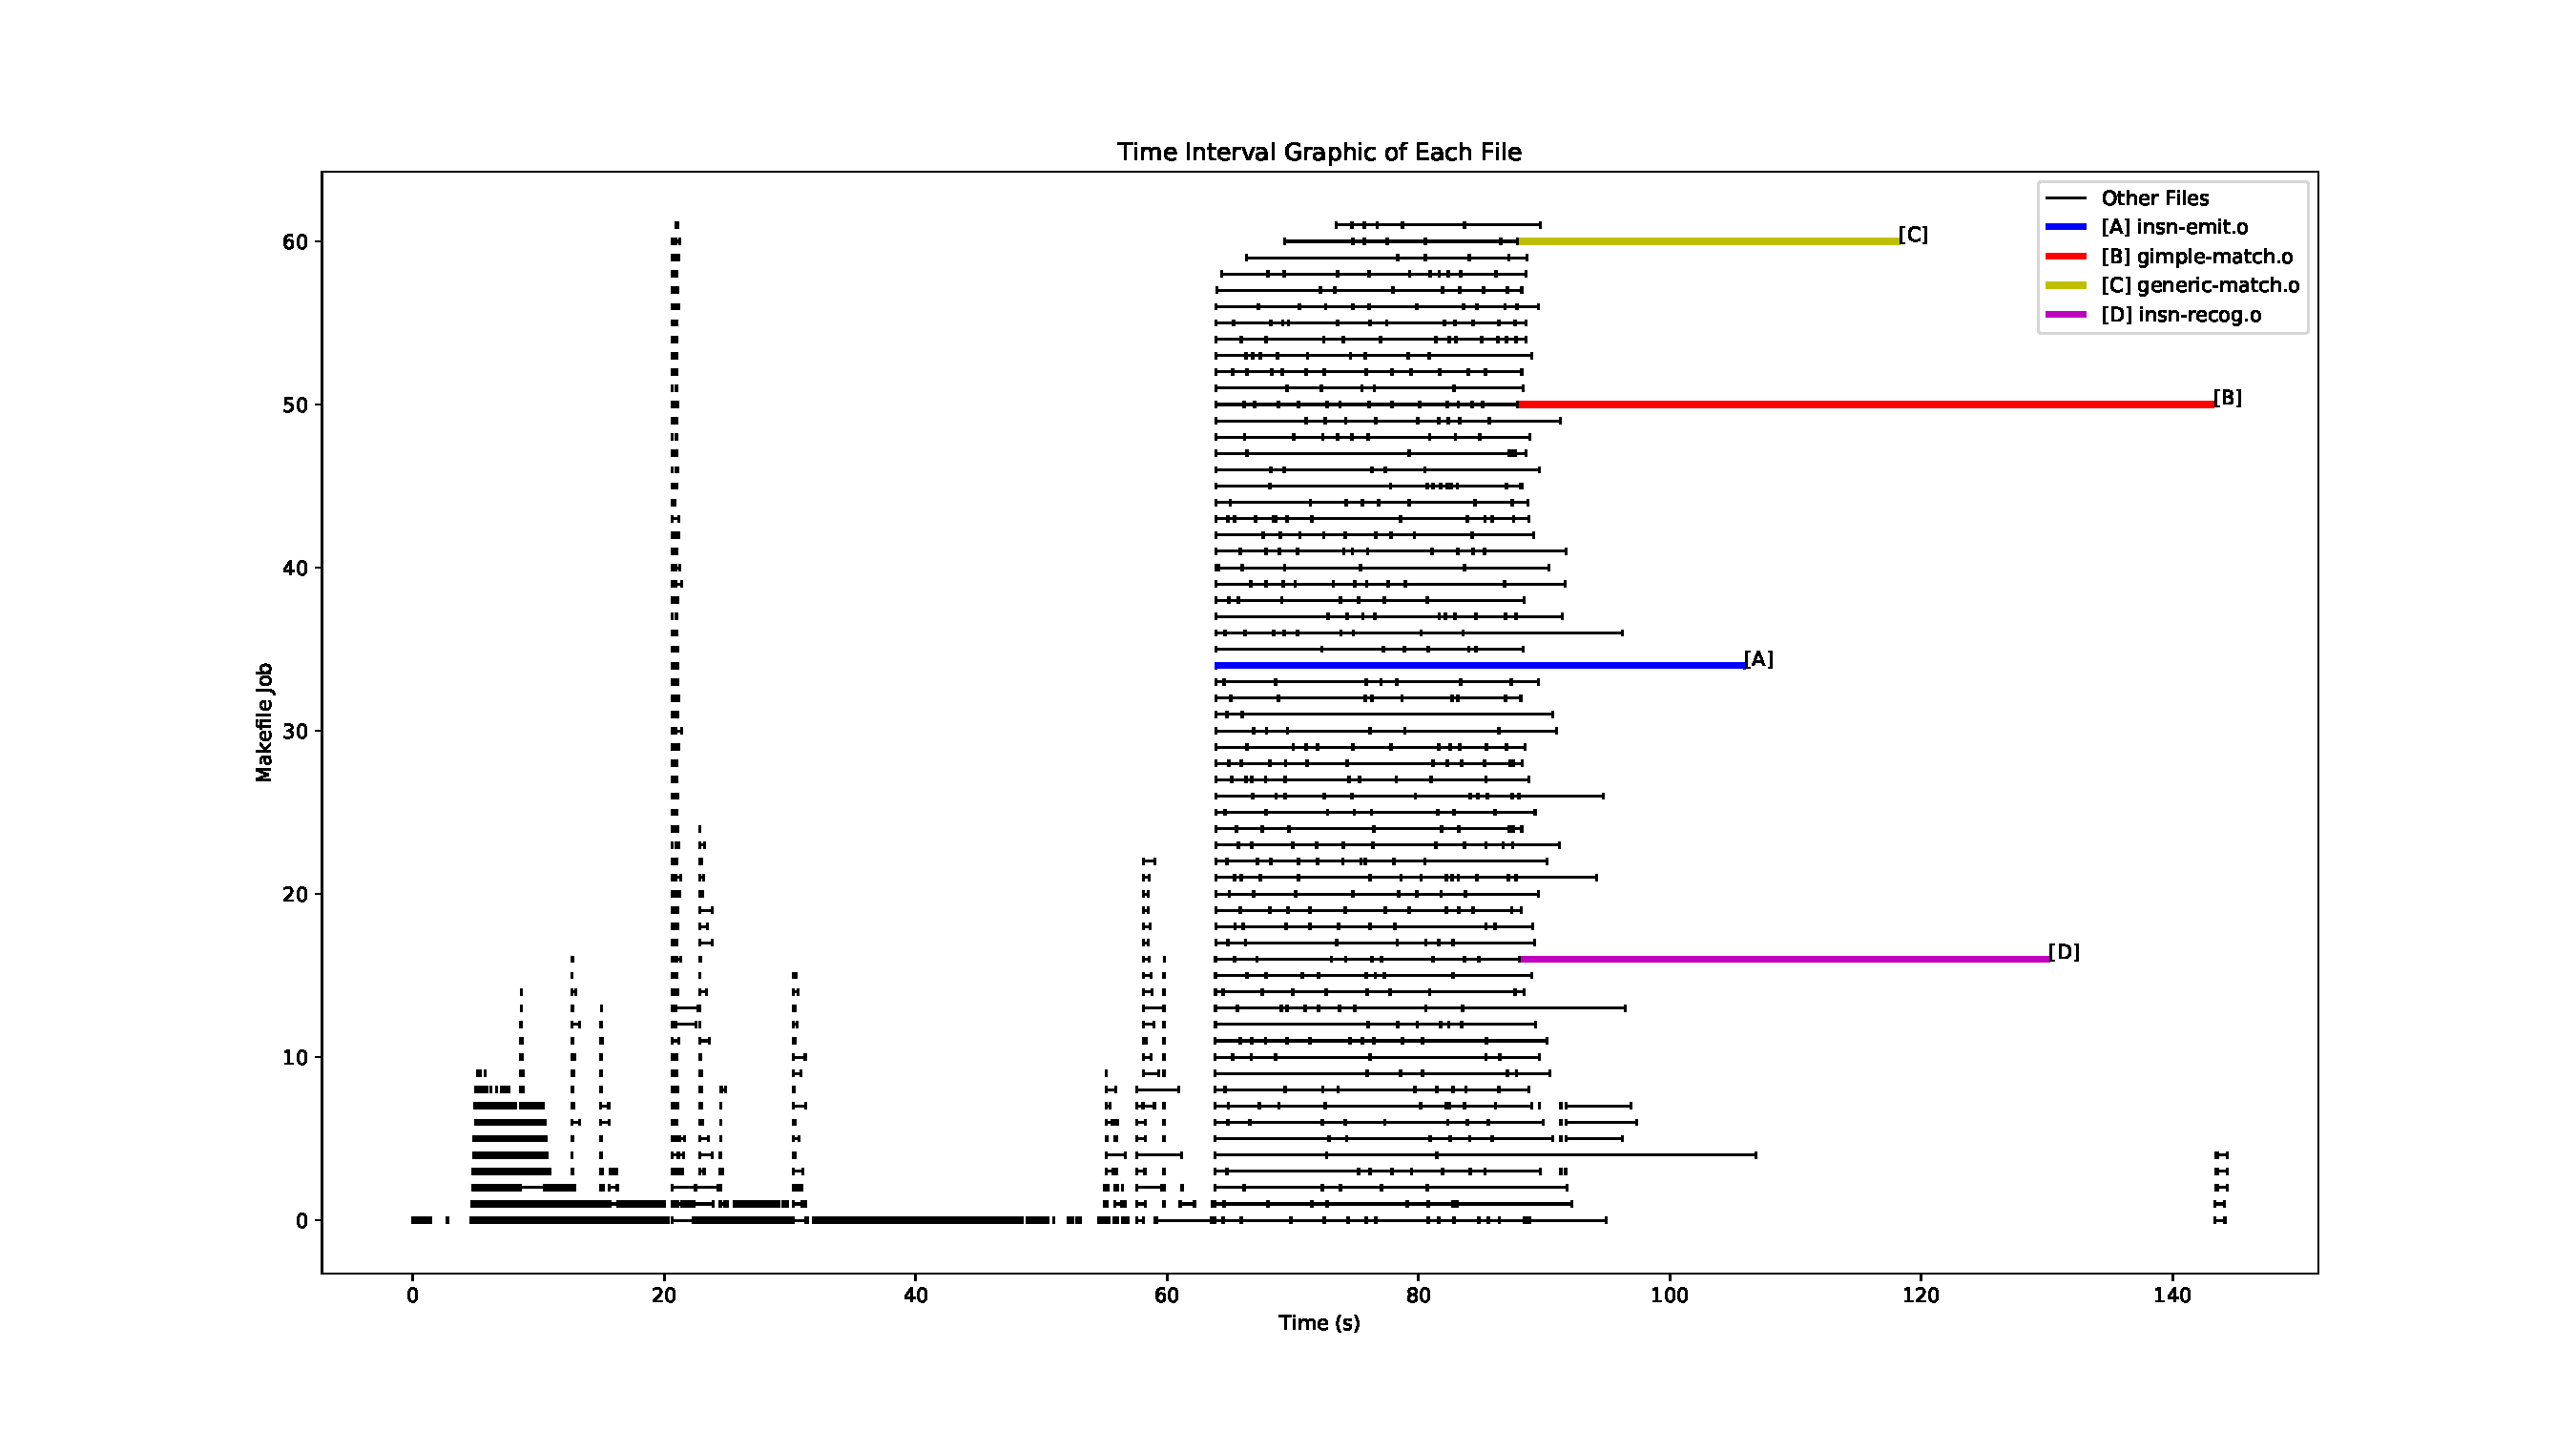
\includegraphics[scale=0.6, angle=-90]{gcc_timer_classic.pdf}
 \caption{Tempo corrido na compilação do GCC em um processador de 64 núcleos. Sem \textit{Bootstrap}}
 \label{fig:analysis_classical}
\end{figure}


%%%%%

\chapter{Conclusions}
\label{chap:conclusions}

We have presented two ways of parallelizing a compiler. Our first approach
involved parallelizing the application of intraprocedural optimizations in
parallel to each function, using threads. Although this predicted a $1.68\times$
speedup on GCC, its implementation showed to be difficult because of the heavy
use of global variables in the software.  We even got to a point where
analyzers such as helgrind and thread sanitizer were not detecting the race
conditions due to the race window being too small. Therefore, this approach may
not be adequate for already existing industrial-scale compilers for adding
parallelism.

However, if we are designing a compiler from the ground up, this approach may
be better from a software engineering perspective, as it becomes easier to add
multithreading to a part of the code that was, at least at some point, designed
with this in mind. We also get the advantage of avoiding the overheads
associated with process creation, such as page copying, etc.

Threading the compiler may also be the only option when parallelizing the
parser or interprocedural analysis, otherwise, there would be a huge amount of
interprocess communication. However, Figure \ref{fig:parallel_estimate} shows
that parsing is not a computer-intensive task. This is already parallel in LTO
by reading the multiple files, therefore this may not be of concern on present
days nor in the short future. However, the interprocess analysis is of concern,
once it is the only sequential step on LTO and may dominate the compilation
time on manycore machines just by being sequential.

On our second approach, we show how to use the already-existing LTO engine in
GCC to compile single files in parallel. The clear advantage of this approach
is how fast we got the first results when compared to threading the compiler,
and how fast we got it into a complete working condition (bootstrap the
compiler, testsuite acceptance, fuzzer testing).

Although the results were better than the threaded version ($1.88\times$ vs. $2.4\times$),
one may argue that the reason for that is due to our threaded implementation
not being as optimized as the LTO based version -- which is true -- and the
contrary must be expected because the cost of launching a thread is smaller
than the cost of launching a process plus all the necessary page copying.
Therefore, we may expect even larger speedups when compared to the LTO version
on optimized implementations.

From now on, we will focus on the LTO implementation results to drive our
conclusions. We archived up to $35\%$ speedup when comparing our results with
the \texttt{make -j64} alone, and no significant slowdown when compared to the
sequential version (even if there was, the developer could simply disable the
parallel compilation if this is observed). The reason for this is the existence
of files with large TU in the GCC project, as shown in Figure
\ref{fig:analysis_classical}, and this result might be interesting when the project
uses autogenerated (blob) C++ files. We also found a small speedup on Git,
which we find interesting because it consists of small files. One explanation
for this is that it does not have enough files to fully populate the manycore
machine's CPU.

As for the electrical energy usage, we show a reduction in power draw by the
CPU when compiling GCC with our options enabled. On Figure \ref{fig:power},
we observe a significant reduction in the peak power usage on the parallel
version. It may be that there is a point when the processor is in partial usage
(not in full usage) and may draw the same amount of power as if it is in full
usage. Therefore, for better energy efficiency, we should use the maximum power
of the CPU in the shortest amount of time to get a task done -- and this will
also save energy --.
%%%%%


%\providecommand\aviso[1]{
  \clearpage
  \null
  \vfill
  \begin{hyphenrules}{nohyphenation}
    \centering\bfseries\Large
    #1\par
  \end{hyphenrules}
  \vfill
  \clearpage
}

\providecommand\avisoFolhasDeRosto{
  \aviso{
    {\huge Você precisa editar os arquivos no diretório ``\texttt{conteudo}''!}
    \par\bigskip\bigskip\bigskip\bigskip
    Para gerar a capa e demais páginas preliminares no formato correto,
    modifique os arquivos ``\texttt{conteudo/paginas-preliminares.tex}'' e
    ``\texttt{conteudo/metadados.tex}'', usando como base os arquivos
    correspondentes no diretório ``\texttt{conteudo-exemplo}''.
  }
}

\providecommand\avisoCapitulos{
  \aviso{
    Insira o conteúdo dos capítulos do seu trabalho no arquivo
    ``\texttt{capitulos.tex}'' do diretório ``\texttt{conteudo}''.
  }
}

\providecommand\avisoApendices{
  \aviso{
    Insira o conteúdo dos apêndices do seu trabalho no arquivo
    ``\texttt{apendices.tex}'' do diretório ``\texttt{conteudo}''.
  }
}

\providecommand\avisoAnexos{
  \aviso{
    Insira o conteúdo dos anexos do seu trabalho no arquivo
    ``\texttt{anexos.tex}'' do diretório ``\texttt{conteudo}''.
  }
}

\providecommand\avisoArtigo{
  \aviso{
    Insira o conteúdo do artigo no arquivo ``\texttt{corpo-artigo.tex}''
    do diretório ``\texttt{conteudo}''. Não se esqueça de consultar
    o exemplo no diretório ``\texttt{conteudo-exemplo}'' para a
    definição do título, autoria etc.
  }
}

\providecommand\avisoApresentacao{
  \begin{frame}{Insira o conteúdo!}
  \aviso{
    Insira o conteúdo da apresentação no arquivo ``\texttt{corpo-apresentacao.tex}''
    do diretório ``\texttt{conteudo}''. Não se esqueça de consultar
    o exemplo no diretório ``\texttt{conteudo-exemplo}'' para a
    definição do título, autoria, estrutura etc.
  }
  \end{frame}
}

\providecommand\avisoPoster{
  \aviso{
    Insira o conteúdo do poster no arquivo ``\texttt{corpo-poster.tex}''
    do diretório ``\texttt{conteudo}''. Não se esqueça de consultar
    o exemplo no diretório ``\texttt{conteudo-exemplo}'' para a
    definição do título, autoria, estrutura etc.
  }
}

%\avisoCapitulos

% Os capítulos de compõem a dissertação/tese, com numeração normal, podem
% ser inseridos diretamente aqui ou "puxados" de outros arquivos.
% Em alguns (raros) casos, pode ser interessante usar \include ao
% invés de \input: https://tex.stackexchange.com/a/32058/183146

%\input{conteudo/01...}
%\par

%\input{conteudo/02...}
%\par

\par


%%%%%%%%%%%%%%%%%%%%%%%%%%%% APÊNDICES E ANEXOS %%%%%%%%%%%%%%%%%%%%%%%%%%%%%%%%

% Um apêndice é algum conteúdo adicional de sua autoria que colabora com a
% ideia geral do texto mas que, por alguma razão, não precisa fazer parte
% da sequência do discurso; por exemplo, a demonstração de um teorema, as
% perguntas usadas em uma pesquisa qualitativa etc.
%
% Um anexo é um documento que não é de sua autoria mas que é relevante para
% a tese; por exemplo, a especificação do padrão que o trabalho discute.
%
% Os comandos appendix e annex reiniciam a numeração de capítulos e passam
% a numerá-los com letras. "annex" não faz parte de nenhuma classe padrão,
% ele foi criado para este modelo (em annex.sty e utils.tex). Se o
% trabalho não tiver apêndices ou anexos, remova estas linhas.

% Este formato está definido na package imeusp-headers
\pagestyle{appendix}

% Sem esta linha, a palavra "Apêndices" no sumário ficava no final da
% primeira página; assim, forçamos uma quebra de página antes.
\addtocontents{toc}{\newpage}
% Apêndices
\appendix

%%!TeX root=../tese.tex
%("dica" para o editor de texto: este arquivo é parte de um documento maior)
% para saber mais: https://tex.stackexchange.com/q/78101/183146

% Os apêndices podem ser inseridos diretamente aqui ou "puxados" de outros
% arquivos.
% Em alguns (raros) casos, pode ser interessante usar \include ao
% invés de \input: https://tex.stackexchange.com/a/32058/183146
%!TeX root=../tese.tex
%("dica" para o editor de texto: este arquivo é parte de um documento maior)
% para saber mais: https://tex.stackexchange.com/q/78101/183146

\chapter{Código-Fonte e Pseudocódigo}
\label{ap:pseudocode}

Com a \textit{package} \textsf{listings}, programas podem ser inseridos
diretamente no arquivo, como feito no caso do Programa~\ref{prog:java},
ou importados de um arquivo externo com o comando
\textsf{\textbackslash{}lstinputlisting}, como no caso
do Programa~\ref{prog:mdcinput}.

% O exemplo foi copiado da documentação de algorithmicx
\begin{program}
  \lstinputlisting[
    language=pseudocode,
    style=pseudocode,
    style=wider,
    functions={},
    specialidentifiers={},
  ]
  {conteudo-exemplo/euclid.psc}

  \caption{Máximo divisor comum (arquivo importado).\label{prog:mdcinput}}
\end{program}

Trechos de código curtos (menores que uma página) podem ou não ser
incluídos como \textit{floats}; trechos longos necessariamente incluem
quebras de página e, portanto, não podem ser \textit{floats}. Com
\textit{floats}, a legenda e as linhas separadoras são colocadas pelo
comando \textsf{\textbackslash{}begin\{program\}}; sem eles, utilize o
ambiente \textsf{programruledcaption} (atenção para a colocação do
comando \textsf{\textbackslash{}label\{\}}, dentro da legenda), como
no Programa~\ref{prog:mdc}\footnote{\textsf{listings} oferece alguns
recursos próprios para a definição de \textit{floats} e legendas, mas
neste modelo não os utilizamos.}:

\begin{programruledcaption}{Máximo divisor comum.\label{prog:mdc}}
  \begin{lstlisting}[
    language=pseudocode,
    style=pseudocode,
    style=wider,
    functions={},
    specialidentifiers={},
  ]
      function euclid(a, b) // The \textbf{g.c.d.} of a and b
          r := a $\bmod$ b
          while r != 0 // We have the answer if r is 0
              a := b
              b := r
              r := a $\bmod$ b
          end
          return b // The \textbf{g.c.d.} is b
      end
  \end{lstlisting}
\end{programruledcaption}

Além do suporte às várias linguagens incluídas em \textsf{listings},
este modelo traz uma extensão para permitir o uso de pseudocódigo,
útil para a descrição de algoritmos em alto nível. Ela oferece
diversos recursos:

\begin{itemize}

    \item Comentários seguem o padrão de C++ (\lstinline{//} e
          \lstinline{/* ... */}), mas o delimitador é impresso
          como ``$\triangleright$''.

    \item ``:='', ``<>'', ``<='', ``>='' e ``!='' são substituídos
          pelo símbolo matemático adequado.

    \item É possível acrescentar palavras-chave além de ``if'', ``and''
          etc. com a opção ``\textsf{morekeywords=\{pchave1,\linebreak[0]{}pchave2\}}''
          (para um trecho de código específico) ou com o comando
          \textsf{\textbackslash{}lstset\{morekeywords=\linebreak[0]{}\{pchave1,pchave2\}\}}
          (como comando de configuração geral).

    \item É possível usar pequenos trechos de código, como nomes de variáveis,
          dentro de um parágrafo normal com \textsf{\textbackslash{}lstinline\{blah\}}.

    \item ``\$\dots\$'' ativa o modo matemático em qualquer lugar.

    \item Outros comandos LaTeX funcionam apenas em comentários; fora, a
          linguagem simula alguns pré-definidos (\textsf{\textbackslash{}textit\{\}},
          \textsf{\textbackslash{}texttt\{\}} etc.).

    \item O comando \textsf{\textbackslash{}label} também funciona em
          comentários; a referência correspondente (\textsf{\textbackslash{}ref})
          indica o número da linha de código. Se quiser usá-lo numa linha sem
          comentários, use \lstinline{///}~\textsf{\textbackslash{}label\{blah\}};
          ``\lstinline{///}'' funciona como \lstinline{//}, permitindo
          a inserção de comandos \LaTeX{}, mas não imprime o delimitador
          (\ensuremath{\triangleright}).

    \item Para suspender a formatação automática, use \textsf{\textbackslash{}noparse\{blah\}}.

    \item Para forçar a formatação de um texto como função, identificador,
          palavra-chave ou comentário, use \textsf{\textbackslash{}func\{blah\}},
          \textsf{\textbackslash{}id\{blah\}}, \textsf{\textbackslash{}kw\{blah\}} ou
          \textsf{\textbackslash{}comment\{blah\}}.

    \item Palavras-chave dentro de comentários não são formatadas
          automaticamente; se necessário, use \textsf{\textbackslash{}func\{\}},
          \textsf{\textbackslash{}id\{\}} etc. ou comandos \LaTeX{} padrão.

    \item As palavras ``Program'', ``Procedure'' e ``Function'' têm formatação
          especial e fazem a palavra seguinte ser formatada como função.
          Funções em outros lugares \emph{não} são detectadas automaticamente;
          use \textsf{\textbackslash{}func\{\}}, a opção ``\textsf{functions=\{func1,func2\}}''
          ou o comando ``\textsf{\textbackslash{}lstset\{functions=\{func1,func2\}\}}''
          para que elas sejam detectadas.

    \item Além de funções, palavras-chave, strings, comentários e
          identificadores, há ``\textsf{specialidentifiers}''. Você pode
          usá-los com \textsf{\textbackslash{}specialid\{blah\}}, com a opção
          ``\textsf{specialidentifiers=\{id1,id2\}}'' ou com o comando
          ``\textsf{\textbackslash{}lstset\{specialidentifiers=\{id1,id2\}\}}''.

\end{itemize}



\par

% Os apêndices podem ser inseridos diretamente aqui ou "puxados" de outros
% arquivos
\chapter{Código-Fonte e Pseudocódigo}
\label{ap:pseudocode}

Com a \textit{package} \textsf{listings}, programas podem ser inseridos
diretamente no arquivo, como feito no caso do Programa~\ref{prog:java},
ou importados de um arquivo externo com o comando
\textsf{\textbackslash{}lstinputlisting}, como no caso
do Programa~\ref{prog:mdcinput}.

% O exemplo foi copiado da documentação de algorithmicx
\begin{program}
  \lstinputlisting[
    language=pseudocode,
    style=pseudocode,
    style=wider,
    functions={},
    specialidentifiers={},
  ]
  {conteudo/euclid.psc}

  \caption{Máximo divisor comum (arquivo importado).\label{prog:mdcinput}}
\end{program}

Trechos de código curtos (menores que uma página) podem ou não ser
incluídos como \textit{floats}; trechos longos necessariamente incluem
quebras de página e, portanto, não podem ser \textit{floats}. Com
\textit{floats}, a legenda e as linhas separadoras são colocadas pelo
comando \textsf{\textbackslash{}begin\{program\}}; sem eles, utilize
o ambiente \textsf{ruledcaption} (atenção para a colocação do comando
\textsf{\textbackslash{}label\{\}}, dentro da legenda), como no
Programa~\ref{prog:mdc}\footnote{\textsf{listings} oferece alguns
recursos próprios para a definição de \textit{floats} e legendas, mas
neste modelo não os utilizamos.}:

\begin{ruledcaption}{Máximo divisor comum.\label{prog:mdc}}
  \begin{lstlisting}[
    language=pseudocode,
    style=pseudocode,
    style=wider,
    functions={},
    specialidentifiers={},
  ]
      function euclid($a,b$) // The \textbf{g.c.d.} of $a$ and $b$
          $r \gets a \bmod b$
          while $r \neq 0$ // We have the answer if $r$ is 0
              $a \gets b$
              $b \gets r$
              $r \gets a \bmod b$
          end
          return $b$ // The \textbf{g.c.d.} is $b$
      end
  \end{lstlisting}
\end{ruledcaption}

Além do suporte às várias linguagens incluídas em \textsf{listings},
este modelo traz uma extensão para permitir o uso de pseudocódigo,
útil para a descrição de algoritmos em alto nível. Ela oferece
diversos recursos:

\begin{itemize}

    \item É possível acrescentar palavras-chave com a opção
          ``\textsf{morekeywords=\{pchave1,\linebreak[0]{}pchave2\}}''
          (para um código específico) ou com o comando
          \textsf{\textbackslash{}lstset\{morekeywords=\linebreak[0]{}\{pchave1,pchave2\}\}}
          (como comando de configuração geral).

    \item É possível usar pequenos trechos de texto, como nomes de variáveis,
          dentro de um parágrafo normal com \textsf{\textbackslash{}lstinline\{blah\}}.

    \item Comentários seguem o padrão de C++ (\lstinline{//} e
          \lstinline{/* ... */}).

    \item ``\$\dots\$'' ativa o modo matemático em qualquer lugar.

    \item Outros comandos LaTeX funcionam apenas em comentários; fora, a
          linguagem simula alguns pré-definidos (\textsf{\textbackslash{}textit\{\}},
          \textsf{\textbackslash{}texttt\{\}} etc.).

    \item O comando \textsf{\textbackslash{}label} também funciona em
          comentários; a referência correspondente (\textsf{\textbackslash{}ref})
          indica o número da linha de código. Se quiser usá-lo numa linha sem
          comentários, use \lstinline{///}~\textsf{\textbackslash{}label\{blah\}};
          ``\lstinline{///}'' funciona como \lstinline{//}, permitindo
          a inserção de comandos \LaTeX{}, mas não imprime o delimitador
          (\ensuremath{\triangleright}).

    \item Para suspender a formatação automática, use \textsf{\textbackslash{}noparse\{blah\}}.

    \item Para forçar a formatação de um texto como função, identificador,
          palavra-chave ou comentário, use \textsf{\textbackslash{}func\{blah\}},
          \textsf{\textbackslash{}id\{blah\}}, \textsf{\textbackslash{}kw\{blah\}} ou
          \textsf{\textbackslash{}comment\{blah\}}.

    \item Palavras-chave dentro de comentários não são formatadas
          automaticamente; se necessário, use \textsf{\textbackslash{}func\{\}},
          \textsf{\textbackslash{}id\{\}} etc. ou comandos \LaTeX{} padrão.

    \item As palavras ``Program'', ``Procedure'' e ``Function'' têm formatação
          especial e fazem a palavra seguinte ser formatada como função.
          Funções em outros lugares \emph{não} são detectadas automaticamente;
          use \textsf{\textbackslash{}func\{\}}, a opção ``\textsf{functions=\{func1,func2\}}''
          ou o comando ``\textsf{\textbackslash{}lstset\{functions=\{func1,func2\}\}}''
          para que elas sejam detectadas.

    \item Além de funções, palavras-chave, strings, comentários e
          identificadores, há ``\textsf{specialidentifiers}''. Você pode
          usá-los com \textsf{\textbackslash{}specialid\{blah\}}, com a opção
          ``\textsf{specialidentifiers=\{id1,id2\}}'' ou com o comando
          ``\textsf{\textbackslash{}lstset\{specialidentifiers=\{id1,id2\}\}}''.

\end{itemize}



\par

\par

% Anexos
\annex

%%!TeX root=../tese.tex
%("dica" para o editor de texto: este arquivo é parte de um documento maior)
% para saber mais: https://tex.stackexchange.com/q/78101/183146

% Os anexos podem ser inseridos diretamente aqui ou "puxados" de outros
% arquivos.
% Em alguns (raros) casos, pode ser interessante usar \include ao
% invés de \input: https://tex.stackexchange.com/a/32058/183146
%!TeX root=../tese.tex
%("dica" para o editor de texto: este arquivo é parte de um documento maior)
% para saber mais: https://tex.stackexchange.com/q/78101/183146

\chapter[Perguntas Frequentes sobre o Modelo]{Perguntas Frequentes sobre o Modelo\footnote{Esta
seção não é de fato um anexo, mas sim um apêndice; ela foi definida desta
forma apenas para servir como exemplo de anexo.}}

\begin{itemize}

\item \textbf{Não consigo decorar tantos comandos!}\\
Use a colinha que é distribuída juntamente com este modelo (\url{gitlab.com/ccsl-usp/modelo-latex/raw/master/pre-compilados/colinha.pdf?inline=false}).

\item \textbf{Por que tantos arquivos?}\\
O preâmbulo \LaTeX{} deste modelo é muito longo; as partes que normalmente não precisam ser modificadas foram colocadas no diretório \texttt{extras}, juntamente com alguns arquivos acessórios. Já os arquivos de conteúdo (capítulos, anexos etc.) foram divididos de maneira que seja fácil para você atualizar o modelo (copiando os novos arquivos ou com um sistema de controle de versões) sem que alterações no conteúdo de exemplo (este texto que você está lendo) causem conflitos com o seu próprio texto.\looseness=-1

\item \textbf{As figuras e tabelas são colocadas em lugares ruins.}\\
Veja a discussão a respeito na Seção~\ref{sec:limitations}.

\item \textbf{Estou tendo problemas com caracteres acentuados.}\\
Veja a discussão a respeito na Seção~\ref{sec:limitations}.

\item \textbf{Existe algo específico para citações de páginas web?}\\
Biblatex define o tipo ``online'', que deve ser usado para materiais com título, autor etc., como uma postagem ou comentário em um blog, um gráfico ou mesmo uma mensagem de email para uma lista de discussão. Bibtex\index{bibtex}, por padrão, não tem um tipo específico para isso; com ele, normalmente usa-se o campo ``howpublished'' para especificar que se trata de um recurso \textit{online}. Se o que você está citando não é algo determinado com título, autor etc. mas sim um sítio (como uma empresa ou um produto), pode ser mais adequado colocar a referência apenas como nota de rodapé e não na lista de referências; nesses casos, algumas pessoas acrescentam uma segunda lista de referências especificamente para recursos \textit{online} (biblatex\index{biblatex} permite criar múltiplas bibliografias). Já artigos disponíveis \textit{online} mas que fazem parte de uma publicação de formato tradicional (mesmo que apenas \textit{online}), como os anais de um congresso, devem ser citados por seu tipo verdadeiro e apenas incluir o campo ``url'' (não é nem necessário usar o comando \textsf{\textbackslash{}url\{\}}), aceito por todos os tipos de documento do bibtex/biblatex.

\item \textbf{Aparece uma folha em branco entre os capítulos.}\\
Essa característica foi colocada propositalmente, dado que todo capítulo deve (ou deveria) começar em uma página de numeração ímpar (lado direito do documento). Se quiser mudar esse comportamento, acrescente ``openany'' como opção da classe, i.e., \textsf{\textbackslash{}documentclass[openany,\dots]\{book\}}.

\item \textbf{É possível resumir o nome das seções/capítulos que aparece no topo das páginas e no sumário?}\\
Sim, usando a sintaxe \textsf{\textbackslash{}section[mini-titulo]\{titulo enorme\}}. Isso é especialmente útil nas legendas (\textit{captions}\index{Legendas}) das figuras e tabelas, que muitas vezes são demasiadamente longas para a lista de figuras/tabelas.

\item \textbf{Existe algum programa para gerenciar referências em formato bibtex?}\\
Sim, há vários. Uma opção bem comum é o JabRef; outra é usar Zotero\index{Zotero} ou Mendeley\index{Mendeley} e exportar os dados deles no formato .bib.

\item \textbf{Posso usar pacotes \LaTeX{} adicionais aos sugeridos?}\\
Com certeza! Você pode modificar os arquivos o quanto desejar, o modelo serve só como uma ajuda inicial para o seu trabalho.

\item \textbf{Como faço para usar o Makefile (comando make) no Windows?}\\
Lembre-se que a ferramenta recomendada para compilação do documento é o \textsf{latexmk}, então você não precisa do \textsf{make}. Mas, se quiser usá-lo, você pode instalar o MSYS2 (\url{www.msys2.org}) ou o Windows Subsystem for Linux (procure as versões de Linux disponíveis na Microsoft Store). Se você pretende usar algum dos editores sugeridos, é possível deixar a compilação a cargo deles, também dispensando o \textsf{make}.\looseness=-1

\item \textbf{Como eu faço para...}\\
Leia os comentários dos arquivos ``tese.tex'' e outros que compõem este modelo, além do tutorial (Capítulo \ref{chap:tutorial}) e dos exemplos do Capítulo \ref{chap:exemplos}; é provável que haja uma dica neles ou, pelo menos, a indicação da \textit{package} relacionada ao que você precisa.

\end{itemize}

\par

%!TeX root=../tese.tex
%("dica" para o editor de texto: este arquivo é parte de um documento maior)
% para saber mais: https://tex.stackexchange.com/q/78101/183146

% Apague as duas linhas abaixo (elas servem apenas para gerar um
% aviso no arquivo PDF quando não há nenhum dado a imprimir) e
% insira aqui o conteúdo dos anexos do seu trabalho (ou deixe este
% arquivo vazio)

\providecommand\aviso[1]{
  \clearpage
  \null
  \vfill
  \begin{hyphenrules}{nohyphenation}
    \centering\bfseries\Large
    #1\par
  \end{hyphenrules}
  \vfill
  \clearpage
}

\providecommand\avisoFolhasDeRosto{
  \aviso{
    {\huge Você precisa editar os arquivos no diretório ``\texttt{conteudo}''!}
    \par\bigskip\bigskip\bigskip\bigskip
    Para gerar a capa e demais páginas preliminares no formato correto,
    modifique os arquivos ``\texttt{conteudo/paginas-preliminares.tex}'' e
    ``\texttt{conteudo/metadados.tex}'', usando como base os arquivos
    correspondentes no diretório ``\texttt{conteudo-exemplo}''.
  }
}

\providecommand\avisoCapitulos{
  \aviso{
    Insira o conteúdo dos capítulos do seu trabalho no arquivo
    ``\texttt{capitulos.tex}'' do diretório ``\texttt{conteudo}''.
  }
}

\providecommand\avisoApendices{
  \aviso{
    Insira o conteúdo dos apêndices do seu trabalho no arquivo
    ``\texttt{apendices.tex}'' do diretório ``\texttt{conteudo}''.
  }
}

\providecommand\avisoAnexos{
  \aviso{
    Insira o conteúdo dos anexos do seu trabalho no arquivo
    ``\texttt{anexos.tex}'' do diretório ``\texttt{conteudo}''.
  }
}

\providecommand\avisoArtigo{
  \aviso{
    Insira o conteúdo do artigo no arquivo ``\texttt{corpo-artigo.tex}''
    do diretório ``\texttt{conteudo}''. Não se esqueça de consultar
    o exemplo no diretório ``\texttt{conteudo-exemplo}'' para a
    definição do título, autoria etc.
  }
}

\providecommand\avisoApresentacao{
  \begin{frame}{Insira o conteúdo!}
  \aviso{
    Insira o conteúdo da apresentação no arquivo ``\texttt{corpo-apresentacao.tex}''
    do diretório ``\texttt{conteudo}''. Não se esqueça de consultar
    o exemplo no diretório ``\texttt{conteudo-exemplo}'' para a
    definição do título, autoria, estrutura etc.
  }
  \end{frame}
}

\providecommand\avisoPoster{
  \aviso{
    Insira o conteúdo do poster no arquivo ``\texttt{corpo-poster.tex}''
    do diretório ``\texttt{conteudo}''. Não se esqueça de consultar
    o exemplo no diretório ``\texttt{conteudo-exemplo}'' para a
    definição do título, autoria, estrutura etc.
  }
}

\avisoAnexos

% Os anexos podem ser inseridos diretamente aqui ou "puxados" de outros
% arquivos.
% Em alguns (raros) casos, pode ser interessante usar \include ao
% invés de \input: https://tex.stackexchange.com/a/32058/183146

%\input{conteudo/...}

\par


%%%%%%%%%%%%%%%%%%%%%%%%%%%%%% SEÇÕES FINAIS %%%%%%%%%%%%%%%%%%%%%%%%%%%%%%%%%%%

% Aqui vão a bibliografia, índice remissivo e outras seções similares.

% Espaço adicional no sumário antes das referências / índice remissivo
\addtocontents{toc}{\vspace{2\baselineskip plus .5\baselineskip minus .5\baselineskip}}

% O comando backmatter desabilita a numeração de capítulos.
\backmatter

% Este formato está definido na package imeusp-headers
\pagestyle{frontback}

% A bibliografia é obrigatória

%%%%%%%%% Bibliografia com natbib (preterido): %%%%%%%%%
%\bibliographystyle{extras/alpha-ime}% citação bibliográfica alpha
%\bibliographystyle{extras/plainnat-ime} % citação bibliográfica textual
%\bibliography{bibliografia}  % associado ao arquivo: 'bibliografia.bib'

%%%%%%%% Bibliografia com biblatex (preferido): %%%%%%%%

\printbibliography[
  title=\refname\label{bibliografia}, % "Referências", recomendado pela ABNT
  %title=\bibname\label{bibliografia}, % "Bibliografia"
  % Inclui a bibliografia no sumário
  heading=bibintoc,
]

% imprime o índice remissivo no documento (opcional)
\printindex

\end{document}
